\PassOptionsToPackage{hyperfootnotes=false}{hyperref}
\PassOptionsToPackage{ngerman,english}{babel}
% The class loads acronym (twbook.cls:114). The abbreviations are spelled out in the
% prose rather than invoked with \ac, so no \label anchors are ever emitted and the
% list's back-links would dangle. nohyperlinks prints the list without them.
\PassOptionsToPackage{nohyperlinks}{acronym}
\documentclass[Master,english,IEEE]{twbook}
\usepackage[utf8]{inputenc}
\usepackage[T1]{fontenc}
\usepackage{longtable,booktabs,multirow,calc,etoolbox}
\usepackage{pdflscape}
\usepackage{footnotehyper}
\usepackage{microtype}
% No [H] placements remain. A forced-here float cannot move, so a figure that does not
% fit abandons the rest of the page. [!htbp] keeps the same figures beside their prose,
% measured as identical or one page earlier, without the half-empty pages.
\usepackage{float}

% Page economy for the shortened review version: allow LaTeX to set more text on a
% page that already carries a float, and to accept a fuller float page, so that
% figures and tables pack against the prose instead of forcing near-empty pages.
\renewcommand{\topfraction}{0.9}
\renewcommand{\bottomfraction}{0.7}
\renewcommand{\textfraction}{0.07}
\renewcommand{\floatpagefraction}{0.8}
\setcounter{topnumber}{3}
\setcounter{bottomnumber}{2}
\setcounter{totalnumber}{4}

\newcommand{\angstrom}{\ensuremath{\text{\AA}}}
\newcounter{tablebeforeaitools}
\providecommand{\tightlist}{%
  \setlength{\itemsep}{0pt}\setlength{\parskip}{0pt}}

\degreecourse{Artificial Intelligence Engineering}
\addbibresource{Literatur.bib}
\ExecuteBibliographyOptions{sorting=none}
\DeclareBibliographyDriver{misc}{%
  \printfield{note}%
  \newunit\newblock%
  \printfield{url}%
  \finentry}

\title{Comparative Analysis of Physics-Based and AI-Based Molecular Docking Tools}
\author{Dominik Mann, PhD BSc}
\hypersetup{
  pdftitle={Comparative Analysis of Physics-Based and AI-Based Molecular Docking Tools},
  pdfauthor={Dominik Mann},
  pdfsubject={Master's thesis in Artificial Intelligence Engineering},
  pdfkeywords={molecular docking, AutoDock Vina, DiffDock, EquiBind, PoseBusters, Orai1}}
\makeatletter
\renewcommand{\@pnumwidth}{2em}
\makeatother
\studentnumber{2410585017}
\supervisor{FH-Prof. Priv.-Doz. Dipl.-Ing.(FH) Dr.\\Bernhard Knapp\\DI Dr. Heinrich Krobath\\Assoz Univ-Prof. DI Dr. Isabella Derler}
\place{Wien}

% The English abstract and its keywords occupy one page. The German translation is
% embedded after an explicit page break because the shared twbook class otherwise
% places \kurzfassung before \outline in an English-language master's thesis.
\outline{Molecular docking predicts protein--ligand binding poses, but physics-based
and artificial-intelligence (AI)-based tools differ in how they search, rank and
represent molecular geometry. This thesis compares three configured blind
whole-protein workflows. These are AutoDock Vina with gnina rescoring, the diffusion
model DiffDock-L with smina optimisation and the equivariant regression model
EquiBind with gnina optimisation. A calibration benchmark of 303 co-crystallised complexes permits
assessment against known poses. The primary endpoint combines physical validity under
the PoseBusters test battery with a heavy-atom root-mean-square deviation of at most
2\angstrom{}. A reference-free case study additionally docks three modulators to four
supplied molecular-dynamics snapshots of the Orai1 calcium channel and evaluates
physical validity, operational placement, pose clustering and interaction
fingerprints. Because workflow variants were selected and evaluated on the same
benchmark, the comparison is descriptive and may be optimistic for unseen targets.

Raw-pose validity was 98.2\% for AutoDock Vina, 24.4\% for DiffDock and 2.9\% for
unguided EquiBind. Local optimisation raised the median per-complex validity yield
from 13.3\% to 93.3\% for DiffDock and from 0\% to 56.7\% for EquiBind. It repaired
local geometry but could not recover an unsampled or grossly misplaced binding mode.
Rank-1 recovery of a pose that was both valid and within 2\angstrom{} of the crystal
ligand reached 34.0\% of complexes for DiffDock, 29.4\% for AutoDock Vina and 15.2\%
for EquiBind. The DiffDock--AutoDock difference was not statistically resolved.
Inspecting the best of the first fifteen poses raised recovery to 55.1\%, 49.8\% and
20.1\%, respectively, while extending the pool to thirty added no more than 0.7
percentage points. The AutoDock rates are a lower bound, because search effort stayed
fixed across whole-receptor boxes. Under the implementation-specific cost accounting, the configured
AutoDock workflow had the highest cost per qualifying pose, whereas EquiBind's short
conditional runtime accompanied successful recovery on only 62 of 303 complexes.

On Orai1, the workflows localised the ligands to markedly different sites. The small,
correlated and reference-free panel supports comparison of workflow behaviour but
does not validate a native pose or binding site. Overall, the results support joint
accuracy-and-validity criteria, local geometry optimisation for the evaluated learned
workflows and explicit inspection of ranking depth. The conclusions apply to the
configured pipelines and hardware rather than to physics-based and AI-based docking
as universal method classes.

\vfill\paragraph*{Keywords:}Molecular docking; Physics-based and AI-based methods;
PoseBusters physical validity; Local pose optimisation; Orai1 calcium channel

\clearpage
\begin{otherlanguage}{ngerman}
\chapter*{Kurzfassung}

Molekulares Docking sagt Bindungsposen von Protein--Ligand-Komplexen voraus.
Physikbasierte und auf künstlicher Intelligenz (KI) beruhende Werkzeuge unterscheiden
sich jedoch in Suche, Reihung und Darstellung der Molekülgeometrie. Diese Arbeit
vergleicht drei konfigurierte Arbeitsabläufe für blindes Ganzprotein-Docking:
AutoDock Vina mit gnina-Rescoring, DiffDock-L mit smina-Optimierung und EquiBind mit
gnina-Optimierung. Ein Kalibrierungsdatensatz aus 303 kokristallisierten Komplexen
ermöglicht die Bewertung anhand bekannter Posen. Der primäre Endpunkt verbindet
PoseBusters-Gültigkeit mit einer Schweratom-RMSD von höchstens 2\angstrom{}. Eine
referenzfreie Fallstudie untersucht zusätzlich drei Modulatoren an vier bereitgestellten
Molekulardynamik-Schnappschüssen des Orai1-Kalziumkanals mittels Gültigkeit, operativer
Platzierung, Posen-Clustering und Interaktionsfingerabdrücken. Da die Varianten auf
demselben Datensatz ausgewählt und bewertet wurden, ist der Vergleich deskriptiv und
kann die Leistung auf unbekannten Zielproteinen überschätzen.

Die Gültigkeit der Rohposen betrug 98,2\% für AutoDock Vina, 24,4\% für DiffDock und
2,9\% für EquiBind ohne Bindungsstellenvorgabe. Lokale Optimierung erhöhte den medianen
Gültigkeitsanteil pro Komplex bei DiffDock von 13,3\% auf 93,3\% und bei EquiBind von
0\% auf 56,7\%. Sie korrigierte lokale Geometrie, nicht jedoch fehlende oder grob
fehlplatzierte Bindungsmodi. Am Rang 1 betrug die Wiederfindungsrate einer gültigen
Pose innerhalb von 2\angstrom{} zur Kristallpose 34,0\% für DiffDock,
29,4\% für AutoDock Vina und 15,2\% für EquiBind; der Unterschied zwischen DiffDock
und AutoDock war statistisch nicht auflösbar. Die beste der ersten fünfzehn Posen
erhöhte diese Raten auf 55,1\%, 49,8\% und 20,1\%; dreißig Posen brachten höchstens
weitere 0,7 Prozentpunkte. Die AutoDock-Raten sind Untergrenzen, da die
Gründlichkeit über alle Ganzprotein-Boxen konstant blieb.
In der implementierungsspezifischen Kostenrechnung hatte
der konfigurierte AutoDock-Ablauf die höchsten Kosten pro qualifizierender Pose.
Die kurze bedingte Laufzeit von EquiBind galt dagegen nur für 62 von 303
erfolgreiche Komplexe.

Für Orai1 lokalisierten die Arbeitsabläufe die Liganden an deutlich unterschiedlichen
Stellen. Das kleine, korrelierte und referenzfreie Panel vergleicht ihr Verhalten,
validiert jedoch weder eine native Pose noch eine Bindungsstelle. Insgesamt sprechen
die Ergebnisse für eine gemeinsame Beurteilung von Genauigkeit und physikalischer
Gültigkeit, für lokale Geometrieoptimierung in den untersuchten KI-Pipelines und für
die explizite Untersuchung der Rangtiefe. Die Schlussfolgerungen gelten für die konfigurierten
Pipelines und die verwendete Hardware, nicht allgemein für physikbasierte oder
KI-basierte Dockingmethoden.

\vfill\paragraph*{Schlagworte:}Molekulares Docking; Physikbasierte und KI-basierte
Methoden; Physikalische PoseBusters-Gültigkeit; Lokale Posenoptimierung;
Orai1-Kalziumkanal
\end{otherlanguage}}

\begin{document}

% Cite all substantively used sources in their reviewed numeric order before the
% first body citation. Every key listed here is also cited somewhere in the text, so the
% printed bibliography contains no uncited entry. Verified 2026-08-23 by diffing this list
% against every \cite in body_main_short.tex and body_appendix_short.tex.
% The following remain in Literatur.bib but are deliberately NOT listed here, because no
% surviving sentence relies on them:
%   ref034, ref039 - never cited in either build.
%   ref089 = ADFRsuite, dropped 2026-08-22 with the Docking Protocols streamline: the
%     only sentence citing it recorded a preparation tool that no reported run used.
%   ref042 (Kong, CRAC antagonists) and ref094 (Zitt, CRAC inhibition) - dropped
%     2026-08-23; the Appendix E pharmacology pass deleted their only citing sentences.
%   ref053 (Zheng, scoring-correction term), ref078 (Durant, interrogating ML scoring
%     functions), ref085 (Wang, differentiable pose optimisation) - dropped 2026-08-23;
%     orphaned by earlier Literature Review and Discussion cuts.
%   ref051 (Noor, VirtuDockDL) - dropped 2026-08-23; its only citing sentence claimed
%     computational efficiency for AI-based docking. Its deep-learning stage is a ligand
%     activity pre-filter, its pose generation is delegated to AutoDock Vina, and it
%     reports no runtime anywhere. That claim now cites ref010 (EquiBind, 0.04 s per
%     complex against 49 s for the fastest search baseline) and ref027 (KarmaDock),
%     which both measure what the sentence asserts.
%   ref074 (Ragoza, ligand pose optimization with atomic grid-based convolutional
%     neural networks) and ref077 (Sunseri, convolutional neural network scoring and
%     minimization in the D3R 2017 community challenge) -
%     dropped 2026-08-29 with the gnina refinement mode. Their only citing sentences
%     described CNN-gradient minimisation, which is no longer part of the analysis.
% If any of these is cited again, re-add its key here in numeric position.
\nocite{ref001,ref002,ref003,ref004,ref005,ref006,ref007,ref008,ref009,ref010,ref011,ref012,ref013,ref014,ref015,ref016,ref017,ref018,ref019,ref020,ref021,ref022,ref023,ref024,ref025,ref026,ref027,ref028,ref029,ref030,ref031,ref032,ref033,ref035,ref036,ref037,ref038,ref040,ref041,ref043,ref044,ref045,ref046,ref047,ref048,ref049,ref050,ref052,ref054,ref055,ref056,ref057,ref058,ref059,ref060,ref061,ref062,ref063,ref064,ref065,ref066,ref067,ref068,ref069,ref070,ref071,ref072,ref073,ref075,ref076,ref079,ref080,ref081,ref082,ref083,ref084,ref086,ref087,ref088,ref090,ref091,ref092,ref093}
\maketitle

\hypertarget{motivation}{%
\chapter{\texorpdfstring{Motivation }{Motivation }}\label{motivation}}

Molecular docking is vital in structure-based drug design, predicting the binding modes of small molecules to target proteins and estimating binding affinities. Computationally modelling protein-ligand interactions enables the screening of vast chemical libraries and thus significantly reduces drug development time and costs \cite{ref007}.

Computational molecular docking emerged in the 1980s from geometric shape-matching methods that predicted ligand binding modes from steric complementarity \cite{ref001}. In 1990, Goodsell and Olson introduced an automated docking procedure based on simulated annealing \cite{ref002}, helping establish the AutoDock family. The combination of empirical interaction models with efficient volumetric energy evaluation enabled flexible-ligand conformational search and increasingly large virtual screens \cite{ref003}. HADDOCK later extended data-guided docking to flexible, multistage modelling of biomolecular complexes \cite{ref004}, \cite{ref005}.

Artificial-intelligence (AI)-enabled protein-ligand docking methods have proliferated in recent years \cite{ref006}. DiffDock-L (hereafter DiffDock) and EquiBind are prominent examples that independent researchers have compared across diverse datasets with physics-based docking tools. Table~\ref{tab:literature-comparisons} in the Appendix (Tools and Functions, AI-Based Molecular Docking) summarises four independent docking evaluations, three of which set physics-based methods against AI-based ones \cite{ref012}, \cite{ref013}, \cite{ref032}, while the fourth benchmarks classical and ligand-guided cross-docking strategies without an AI arm and so enters the table as a non-AI reference rather than as a physics-versus-AI comparison \cite{ref033}. Despite reported gains in speed or accuracy, comparisons between classical and AI-based docking carry recurring limitations, namely evaluation from a selected output pose \cite{ref012}, \cite{ref013}, \cite{ref035}, search conditions that are not matched across the competing methods \cite{ref011}, \cite{ref035}, and the absence of post-docking optimisation together with explicit physical-validity screening \cite{ref012}, \cite{ref035}. None of the tabulated evaluations addresses Orai1. AutoDock Vina is retained here as an established baseline rather than assumed to be universally superior. The following research questions therefore guide this thesis.

\begin{enumerate}
\item[\textbf{RQ1}] How do AutoDock Vina, DiffDock and EquiBind differ in physical validity, near-nativeness and ranking depth?
\item[\textbf{RQ2}] How does post-docking optimisation affect the physical validity and near-nativeness of the predicted poses?
\item[\textbf{RQ3}] How do the computational costs of AutoDock Vina, DiffDock and EquiBind compare?
\item[\textbf{RQ4}] What opportunities and limitations do AutoDock Vina, DiffDock and EquiBind present for blind whole-protein docking?
\end{enumerate}

Each question is posed about the three workflows as configured here rather than about physics-based and AI-based docking as method classes, because every workflow couples a search or generative model to a particular preparation, refiner and ranking rule and cannot be separated from them. The same three workflows are additionally applied to a reference-free Orai1 panel, which has no crystallographic pose and therefore supports an operational comparison rather than an accuracy measurement. None of the endpoints is a claim about thermodynamic or time-dependent stability, which docking does not test.

\hypertarget{literature-review}{%
\chapter{\texorpdfstring{Literature Review }{Literature Review }}\label{literature-review}}

\hypertarget{molecular-docking-process}{%
\section{Molecular Docking Process}\label{molecular-docking-process}}

Molecular docking aims to predict geometry, bound pose and interactions of small-molecule ligands and target proteins. Ligands often induce conformational changes in the protein, altering its functional state and triggering downstream biological effects \cite{ref016}.

Small-molecule binding at protein pockets modulates functions such as catalysis, structural organisation and cellular signalling, which makes proteins central targets in drug discovery \cite{ref014}, \cite{ref015}.

\hypertarget{physics-based-molecular-docking}{%
\subsection{Physics-Based Molecular Docking}\label{physics-based-molecular-docking}}

Physics-based protein-ligand docking is a computational process that predicts how ligands (small molecules) bind to proteins at the atomic level. This prediction is vital for understanding molecular recognition mechanisms. Next to predicting ligand conformation and position (sampling), binding affinities are assessed (scoring) in the docking process. The classical workflow proceeds in five stages, which are set out in Figure~\ref{fig:literature-docking-workflow} in the Appendix (Tools and Functions, AutoDock Vina, Docking Procedure).

\hypertarget{autodock-vina}{%
\subsubsection{AutoDock Vina}\label{autodock-vina}}

AutoDock Vina couples an efficient global search engine to an interchangeable empirical scoring function \cite{ref022}, \cite{ref023}. Two functions are relevant here, namely the original Vina function and the later Vinardo reparametrisation, both selectable within the same program \cite{ref023}. The engine generates random poses inside a user-defined search box, refines them by iterated local search over precomputed interaction grids, clusters the survivors by RMSD and returns the lowest-energy representatives. The chosen function is evaluated together with its gradient, so each pose is minimised during the search. No separate post-docking optimisation is needed.

The Vina function itself is a weighted sum of two attractive Gaussian steric terms, a repulsive parabola, a hydrophobic term and a hydrogen-bond term, divided by a factor growing with the number of rotatable bonds. Its six weights were fitted empirically rather than derived from first principles \cite{ref022}. The rotatable-bond divisor is a conformational-entropy surrogate that down-weights ligands paying a larger flexibility cost on binding. Neither an explicit electrostatic term nor an explicit desolvation term appears in the sum, so charge complementarity and solvent displacement enter only implicitly through the fitted weights. Vinardo keeps those families of terms but drops the second, longer-range Gaussian that tended to seat ligands too deeply in the pocket. Vinardo\textquotesingle s parameters were selected on redocking behaviour rather than on correlation with measured affinities \cite{ref073}. Switching between them therefore changes only the objective that the shared engine minimises and ranks, which keeps the two directly comparable. The full protocol, scoring equations and fitted weights for both functions are reproduced in the Appendix (Tools and Functions, AutoDock Vina).

\hypertarget{ai-based-molecular-docking}{%
\subsection{AI-Based Molecular Docking}\label{ai-based-molecular-docking}}

AI-based docking tools learn interaction patterns from large sets of protein-ligand complexes rather than searching an engineered energy landscape. They tend to be computationally efficient, which improves scalability for large-scale virtual screening \cite{ref010}, \cite{ref027}. Three main strategies exist. Diffusion models such as DiffDock \cite{ref024} treat docking as generative sampling. Direct pose prediction such as EquiBind \cite{ref009}, \cite{ref010} regresses the bound pose with an SE(3)-equivariant network. Hybrids pair a classical conformational search with an AI-driven score. A fuller survey, including distance-map, regression-based and co-folding models, is given in the Appendix (Tools and Functions, AI-Based Molecular Docking).

\hypertarget{diffdock}{%
\subsubsection{DiffDock}\label{diffdock}}

DiffDock treats pose prediction as generative sampling rather than optimisation of a hand-crafted energy function \cite{ref024}. Protein and ligand are represented as graphs and the pose is parameterised by translation, rotation and internal torsions. Training corrupts known poses by adding noise to those variables. At inference an SE(3)-equivariant network denoises random placements over several steps toward a high-probability bound conformation. The equivariance keeps predictions consistent under rigid motions. Because sampling is stochastic, DiffDock returns several plausible poses, which suits multimodal docking landscapes. Its scoring has two learned components. A diffusion score model steers the denoising trajectory. A confidence model ranks poses by whether they fall below a 2\angstrom{} RMSD threshold rather than by an affinity-like energy. Performance therefore depends heavily on the training data and on confidence calibration \cite{ref024}. Full details are given in the Appendix (Tools and Functions, DiffDock).

\hypertarget{equibind}{%
\subsubsection{EquiBind}\label{equibind}}

EquiBind predicts the bound pose directly in a single forward pass of an SE(3)-equivariant network \cite{ref010}. Interaction-aware equivariant message passing between the protein and ligand graphs lets the network infer both where the ligand binds and how it is oriented without a predefined site. It uses no separate scoring function at inference. Training instead applies losses that penalise geometric error to the experimental reference. The criteria for a good pose are held in the trained weights rather than in an analytic energy function \cite{ref010}. Each forward pass returns a pose without a confidence value or an affinity-like number, so any ranking must come from outside the model. Dropping both stochastic search and repeated denoising gives it a large runtime advantage. Full details are given in the Appendix (Tools and Functions, EquiBind).

\hypertarget{optimization-tools}{%
\subsection{Optimisation Tools}\label{optimization-tools}}

\hypertarget{smina}{%
\subsubsection{smina Local Optimisation}\label{smina}}

smina and gnina are used as lightweight local-optimisation tools that relax generated poses and, in some arms, additionally re-order them by the resulting score. The two roles are separable, and the one that applies is stated for each arm where that arm is introduced. smina is a fork of AutoDock Vina developed by Koes et al.\ that keeps Vina\textquotesingle s default scoring function and its global search while exposing the individual energy terms for reweighting \cite{ref055}. The energy it optimises is therefore the Vina objective described above. Beyond full docking it exposes a fast local-minimisation mode that relaxes a supplied pose into the nearest energy minimum without repeating the conformational search. This makes it suited to post-docking optimisation \cite{ref057}.

\hypertarget{gnina}{%
\subsubsection{gnina Rescoring}\label{gnina}}

gnina is a fork of smina, so both share the Vina docking algorithm. The Vina energy is the quantity optimised during search \cite{ref056}, \cite{ref067}, \cite{ref068}. gnina differs in ranking, replacing the hand-crafted score with a learned one. An ensemble of convolutional neural networks rescores the poses. Each network reads a three-dimensional grid of Gaussian atom-type densities built with libmolgrid \cite{ref076} and is trained to distinguish poses within 2\angstrom{} RMSD of the native mode from poses outside it (CNNscore) \cite{ref075}. Each also uses a regression head that predicts a binding constant on a pK scale (CNNaffinity) \cite{ref059}, \cite{ref056}, \cite{ref067}. Full details appear in the Appendix (Tools and Functions, Optimisation Tools).

The learned score is applied here to reorder an existing pose set rather than to supply the objective that moves its atoms \cite{ref056}, \cite{ref058}. In rescoring, the inherited quasi-Newton minimiser first drives the pose to a local minimum of the empirical function. Only then are the convolutional networks evaluated and the pose set reordered by the learned score \cite{ref056}. Coordinates do shift, but that displacement is produced by the empirical objective exactly as smina would produce it. The network changes the ranking rather than the geometry.

Rescoring supplies the deep-learning pipelines with geometric repair. It also supplies the ranking that EquiBind does not otherwise provide, whereas DiffDock already orders its own poses by confidence and keeps that order throughout. The AutoDock variants receive the same pass as a post-hoc step over the poses of a completed search, where it both repairs local geometry and re-orders the poses by CNN affinity. The protocols are set out in the Appendix (Docking Protocols, AutoDock Vina).

\hypertarget{methods}{%
\chapter{\texorpdfstring{Methods }{Methods }}\label{methods}}

This exploratory study aims to compare the performance of physics-based AutoDock Vina with the diffusion model DiffDock and the regression model EquiBind. The two latter deep-learning methods are coupled to lightweight physics-based local optimisation with smina or gnina. Their comparative performance informs docking on Orai1, for which no reference ligand pose is available.

\hypertarget{datasets}{%
\section{Datasets}\label{datasets}}

The study is based on crystal-referenced calibration and reference-free Orai1 dataset to evaluate the poses produced by AutoDock Vina, DiffDock and EquiBind.

\protect\hypertarget{_Toc235735885}{}{}

\hypertarget{calibration-dataset}{%
\subsection{Calibration Dataset}\label{calibration-dataset}}

The calibration dataset includes 308 high-quality protein--ligand crystal complexes of the PoseBusters benchmark \cite{ref035}, retrieved from the Protein Data Bank \cite{ref043}. The post-2021 release criterion excludes published training data of AI docking models and spans broad chemical and structural properties, with medians of 24 heavy atoms, 359~Da molecular weight and five rotatable bonds. Receptor preparation stripped waters, ions, metals and cofactors for the AutoDock and DiffDock arms, and 78 of the 303 analysed complexes place a metal within 5\angstrom{} of the crystal ligand, so the rates reported for those two arms are apo-like rates (Appendix~\ref{autodock-vina-2}). Appendix~\ref{dataset} describes the dataset in full (Table~\ref{tab:appendix-ligand-distribution}).

\hypertarget{experimental-dataset}{%
\subsection{Experimental Dataset}\label{experimental-dataset}}

The experimental dataset examines the calcium release-activated calcium (CRAC) channel Orai1, for which no crystallographic ligand pose is available.

Four receptor states are used rather than one because all three pipelines hold the receptor rigid, and conformational variation can therefore enter only through separate receptor structures. The regions implicated for small-molecule modulators on Orai1 are the mobile non-pore-lining transmembrane interfaces \cite{ref072} and the extracellular calcium-accumulating region \cite{ref038}, neither of which is a rigid buried pocket, which makes any single snapshot unrepresentative. Retaining the starting structure Fr0 alongside the three later frames additionally contrasts one pre-dynamics starting geometry with three thermally sampled ones, a contrast that matters because the learned pipelines were trained on crystallographic receptors. Appendix~\ref{orai1-receptor-model} quantifies the spread the four states actually span and states what this design does and does not support.

The Orai1 molecular-dynamics snapshots, Fr0, Fr300, Fr400 and Fr499, represented limited receptor flexibility \cite{ref038}, \cite{ref072}. The PDBQT converter added polar hydrogens by its geometric rules rather than a titration model, except on the AutoDock copy of Fr0, which a preparation fallback repaired, protonated at pH 7.0 and energy-minimised before conversion (Appendix~\ref{orai1-receptor-model}). The three compounds were docked as neutral species. These are 2abp-NH2 (the neutral protonation state of 2-APB and hereafter called 2-APB), GSK-7975A \cite{ref041}, \cite{ref070} and Synta-66 \cite{ref071}. Because no titration model was applied to the ligands, these forms are modelling choices rather than predictions of physiological protonation. The externally supplied optimised geometries lacked records of both the optimisation program and its level of theory (Appendix~\ref{experimental-ligand-pharmacology}).

The three compounds are tool compounds for store-operated calcium entry, in which STIM1 activates Orai1 after depletion of the endoplasmic-reticulum calcium store. Their mechanisms and scaffolds differ, imposing unequal challenges on the docking tools. GSK-7975A and Synta-66 act at or near the extracellular pore mouth and selectivity filter rather than in the conduction pathway, making a chemically valid pose inside the transmembrane slab implausible for these compounds. Appendix~\ref{experimental-ligand-pharmacology} details their pharmacology, sites, selectivity liabilities and mechanistic differences. These differences make the biologically defensible region compound-dependent.

\hypertarget{evaluation-metrics}{%
\section{Evaluation Metrics}\label{evaluation-metrics}}

The evaluation distinguishes pose placement, internal form and physical admissibility before combining them.

\hypertarget{near-nativeness-rmsd-2uxe5}{%
\subsection{\texorpdfstring{Near-Nativeness (RMSD \ensuremath{\leq} 2\angstrom{})}{Near-Nativeness (RMSD <= 2 Angstrom)}}\label{near-nativeness-rmsd-2uxe5}}

Near-nativeness is the symmetry-corrected heavy-atom root-mean-square deviation (RMSD) between a docked pose and the crystallographic ligand:

\[\text{RMSD=}\sqrt{\frac{\sum_{i = 1}^{N}d_{i}^{\text{2}}}{N}}\]

where N is the number of heavy atoms and d\textsubscript{i} is the Euclidean distance between the i-th corresponding atoms in the docked and crystallographic positions. RMSD is computed in place without superposition onto the crystal ligand. A pose is accurate at the conventional threshold of RMSD \ensuremath{\leq} 2\angstrom{} \cite{ref022}, \cite{ref050}. Graph-isomorphism mapping selects among symmetry-equivalent atom assignments \cite{ref044}, an established alternative to bipartite matching \cite{ref048}, and prevents symmetric ligands from receiving inflated errors. The mapping resolves topological symmetry but does not interchange the oxygens of conjugated terminal groups such as carboxylates and phosphates. The reported value is therefore never smaller than a fully symmetrised RMSD on any of the poses analysed here, so near-native counts are not overstated. Substituting the fully symmetrised value into the rank-1 gate adds three recovered complexes across the three tools and removes none (Appendix~\ref{supplementary-statistics}). Because a geometrically accurate pose can still be chemically distorted or sterically impossible, the analysis pairs accuracy with PoseBusters physical validity (PB-valid) \cite{ref035}.

The headline crystal-referenced criterion, valid-near-native, requires both RMSD \ensuremath{\leq} 2\angstrom{} and PB-validity. Form is scored separately for the reason given below. The term also distinguishes this criterion from the operational usable-pose rule for Orai1.

A tool can generate a near-native pose without ranking it first. Accuracy is therefore reported for the realistic rank-1 pose and for the oracle (best) pose anywhere in the output. Per-rank success and cumulative recovery within the first k poses use the gap between these regimes to distinguish ranking from sampling quality.

Binding-site recovery provides a coarser measure of whether the ligand reaches the correct pocket. It is assessed by clustering poses across tools and against the crystallographic pocket, a resolution also applicable to reference-free Orai1.

\hypertarget{form-kabsch-rmsd-1-uxe5}{%
\subsection{\texorpdfstring{Form (Kabsch RMSD \ensuremath{\leq} 1\angstrom{})}{Form (Kabsch RMSD <= 1 Angstrom)}}\label{form-kabsch-rmsd-1-uxe5}}

In-place RMSD combines placement and internal-form errors. Best-fit Kabsch superposition separates them.

With both ligands translated to a common centroid and R the optimal proper rotation obtained by the Kabsch singular-value-decomposition construction \cite{ref062}, the form error is

\[\text{RMSD}_{\text{form}}\text{=}\sqrt{\frac{\sum_{i = 1}^{N}\left\| Rx_{i}\text{-}y_{i} \right\|^{\text{2}}}{N}}\]

where x\textsubscript{i} and y\textsubscript{i} are the centred coordinates of the i-th heavy-atom pair and N is the number of heavy atoms. The value is obtained from the PoseBusters implementation \cite{ref035}.

% RESOLVED 2026-08-16: the analysis code does not share one mapping, since the in-place value comes from RDKit CalcRMS and the Kabsch value from GetBestRMS (posebusters/modules/rmsd.py), each minimising over symmetry mappings independently, so the decomposition is described here as approximate.
For a fixed atom correspondence, rigid superposition gives in-place\textsuperscript{2} = placement\textsuperscript{2} + form\textsuperscript{2} per pose, with placement derived as \(\sqrt{\text{in-place}^{2}-\text{form}^{2}}\). Here, however, the in-place and best-fit values independently minimise over symmetry-equivalent atom mappings and may select different mappings for the same pose. The decomposition is therefore approximate, and placement is a residual diagnostic rather than an independently measured component. Form recovery is reported independently of the 2\angstrom{} in-place threshold. It is conditioned on PoseBusters validity in the depth-recovery figures but reported over all produced poses in Table~\ref{tab:results-pose-production}. A pose is form-correct at Kabsch RMSD \ensuremath{\leq} 1\angstrom{}. That bound was fixed before analysis as a conformer-level counterpart to the cited 2\angstrom{} in-place threshold, half its value and applied to only one of the two components of the in-place deviation. No published convention is claimed for it. Table~\ref{tab:results-near-native-form} in Appendix~\ref{supplementary-statistics} resolves form recovery over ten thresholds from 0.25 to 2.5\angstrom{}, so the sensitivity to this choice can be read directly.

Directional contacts such as hydrogen bonds, hydrophobic burial, \ensuremath{\pi}-stacking and salt bridges depend on bound conformation, so reproducing native interactions requires the correct form. The separation also localises the limiting stage. A placement-limited pose (right shape, wrong position) implicates pocket targeting, whereas a form-limited pose implicates conformer generation or refinement. Figures~\ref{fig:results-r2a} to \ref{fig:results-r3} present the tool-specific analysis.

\hypertarget{physical-and-chemical-validity-posebusters-checks}{%
\subsection{Physical and Chemical Validity (PoseBusters Checks)}\label{physical-and-chemical-validity-posebusters-checks}}

RMSD can be low for chemically distorted or sterically clashing poses, a failure mode the original PoseBusters study attributes to AI-based methods \cite{ref035}. Every pose was therefore evaluated with the PoseBusters ``dock'' battery and counted as PB-valid only if it passed all twenty-two applicable checks (Table~\ref{tab:appendix-posebusters-checks}). PoseBusters provides five additional checks that require a co-crystallised reference ligand. These are identity tests for molecular formula, bond graph, tetrahedral chirality and double-bond stereochemistry, and an RMSD threshold. No reference molecule was supplied because the analysis evaluates near-nativeness separately. Including the reference-dependent RMSD test would merge these two axes. PB-valid therefore denotes the same twenty-two reference-free checks in the calibration and Orai1 datasets.\footnote{Providing a co-crystallised reference was measured post hoc across all poses of the whole-protein benchmark run. Applying them only reduces DiffDock recovery in Table~\ref{tab:results-depth-recovery} by one complex at rank-1 and by two at top-15 and top-30. AutoDock and EquiBind remain unchanged.}

The Results decompose failures into three groups. Chemical validity covers parsing, sanitisation and connectivity. Intramolecular geometry covers bond lengths, angles, flatness, internal clashes and strain. Intermolecular validity covers minimum distances and volume overlaps with proteins, cofactors and waters. The cofactor and water checks are inert on the AutoDock and DiffDock arms, whose prepared receptors hold neither. Only EquiBind is screened against the deposited receptor and its retained heteroatom records (Table~\ref{tab:appendix-posebusters-checks}).

\hypertarget{operational-placement-transmembrane-exclusion}{%
\subsection{Operational Placement (Transmembrane Exclusion)}\label{operational-placement-transmembrane-exclusion}}

Because Orai1 has no crystallographic ligand, an operational placement rule replaces near-nativeness. A pose is usable when it is PoseBusters-valid, placed on the receptor and outside the transmembrane exclusion slab.

Orai1 is a hexamer whose six TM1 helices line the pore from the cytosolic basic residue Arg91 to the extracellular selectivity filter Glu106. The band between these residue rings is the membrane-spanning ion-conduction region rather than a druggable surface pocket. The exclusion slab is the set of points between the planes of the six Arg91 C\ensuremath{\alpha} atoms and the six Glu106 C\ensuremath{\alpha} atoms, without padding. A pose is classified as transmembrane and excluded from the usable count when its heavy-atom centroid lies within this slab. Appendix~\ref{docking-protocols} specifies the envelope thresholds, pore-axis construction, equations and interpretive limits.

\hypertarget{clustering}{%
\subsection{Clustering}\label{clustering}}

Clustering uses each pose\textquotesingle s heavy-atom centroid to compare site placement, while full-atom RMSD remains a separate pose-quality measure. For each complex, centroids from all three tools are pooled into a pairwise Euclidean distance matrix and partitioned by complete-linkage agglomerative clustering at an 8\angstrom{} cut, the physical scale of a binding pocket. The number of clusters is inferred and may be one. Complete linkage makes the cut deterministic by bounding each cluster\textquotesingle s internal spread at the same distance. Candidate pockets are ranked by cross-tool agreement rather than raw pose count, preventing a high-throughput tool from dominating the ranking through output volume alone.

The same 8\angstrom{} centroid clustering is applied within each Orai1 MD frame. All three tools dock into the same receptor coordinates for a given frame. The one exception is the AutoDock copy of Fr0, which was energy-minimised in place and whose C\ensuremath{\alpha} atoms moved by 0.64\angstrom{} (Appendix~\ref{orai1-receptor-model}). The poses of all three tools therefore already share one coordinate system and the within-frame site metrics apply no symmetry folding. Because the four snapshots occupy different coordinate systems, across-frame comparisons instead represent each pose by the receptor residues within 4\angstrom{} of the ligand, folded over Orai1\textquotesingle s six-fold symmetry, rather than by absolute position. Folding is confined to that across-frame representation. This permits comparison without superposition. Within each frame--ligand unit, a tool\textquotesingle s consensus site is the centroid of its largest pose cluster. Cross-tool agreement is the Euclidean distance between two consensus sites. A pair agrees at \ensuremath{\leq} 5\angstrom{}. This pocket-scale threshold is more permissive than pose-level RMSD because it compares pocket centres rather than atom positions.

Silhouette, Calinski-Harabasz, Davies-Bouldin and nearest-cluster separation are reported only for cases with at least two clusters. Compactness also applies to a single cluster, while bootstrap Jaccard overlap measures reproducibility under resampling. Crystal-site recovery is assessed separately at the prespecified 4\angstrom{} centroid threshold. The cluster nearest the crystal is not automatically counted as recovered.

\hypertarget{interaction-fingerprints-metric}{%
\subsection{Interaction Fingerprints}\label{interaction-fingerprints-metric}}

PandaMap profiles the contacts of each retained pose \cite{ref090} using interaction types in the style of the Protein-Ligand Interaction Profiler (PLIP) \cite{ref054}, but without PLIP\textquotesingle s angular criteria in this execution path. Each contact becomes a key combining its interaction class and receptor residue. The set of keys is the pose fingerprint. Because the keys include residue numbers, every pose and reference is profiled against one common author-numbered receptor per target, preventing receptor renumbering from eliminating apparent matches. Profiling includes only PoseBusters-valid poses and, for Orai1, only poses outside the transmembrane slab. The retained depth is capped at the top five ranked poses per calibration complex and the top three per Orai1 frame--ligand unit. A tool\textquotesingle s fingerprint for a complex is the union across its retained poses, yielding one value per tool and complex. Appendix~\ref{interaction-fingerprints} defines the interaction classes, distance thresholds and receptor canonicalisation.

The comparison differs by dataset. On the calibration benchmark, each tool is compared with the crystal-ligand fingerprint using mean Jaccard overlap and rank-resolved precision, recall and F1 for native-contact recovery. Jaccard incorporates both shared and non-shared contacts and therefore measures similarity rather than recall. On Orai1, fingerprints are compared between tools and between experimental and control ligand panels. Outputs comprise contacts per pose, mean counts by interaction class, per-residue hot-spot profiles and Jaccard overlap of engaged residues, both with and without requiring the interaction class to match. The corresponding results appear under Interaction and Contact Analysis.

\hypertarget{computational-cost}{%
\subsection{Computational Cost}\label{computational-cost}}

Computational cost is reported per pose that is PoseBusters-valid and within 2\angstrom{} of the crystal ligand, charging each pipeline against successful benchmark poses. Elapsed wall-clock time, CPU-core-seconds and GPU-seconds are recorded separately. CPU and GPU currencies are not combined because multithreaded processor stages and single-GPU stages consume different resources, whereas elapsed times of consecutive stages are summed. Multistage pipelines are timed by stage in the same run, separating the cost of learned rescoring from the search it re-ranks.

The headline figure is charged device occupancy, defined identically for every pipeline as CPU-core-seconds divided by the 32 hardware threads of the workstation plus GPU-seconds. Dividing by the thread count converts a saturating processor stage into the time it occupied the machine, so what is added to GPU occupancy is a time rather than a resource-second and the rule above holds. Charging occupancy rather than elapsed time also stops work that merely ran with more concurrency from appearing cheaper.

The same measurements are also reported per generated pose and attempted docking because tool rankings depend on the denominator. Appendix~\ref{docking-protocols} records the workstation and device used for each stage. Pose Production Costs reports the measurements.

\hypertarget{statistical-analysis}{%
\subsection{Statistical Analysis}\label{statistical-analysis}}

All inferential statements follow Appendix~\ref{supplementary-statistics}. Tests are two-sided at nominal \ensuremath{\alpha = 0.05}, except the equivalence analysis, which uses two one-sided tests at the same \ensuremath{\alpha} and is therefore evaluated with a 90\% interval. No test assumes normality. Each comparison includes an effect size or the underlying paired proportions, separating the magnitude of a difference from its statistical uncertainty.

The inferential unit is fixed by design. For the calibration benchmark it is the complex, with all poses reduced to one value per complex and tool. For Orai1 it is the frame--ligand pair, removing the nesting of poses within a docking run. These pairs are not independent because the four frames for each ligand are snapshots of one receptor. The effective number of independent experimental observations is therefore three ligands. Orai1 cross-panel contrasts are not treated as established findings. Each is re-tested at ligand level in a sensitivity analysis reported with its result, except per-residue hot-spot frequencies, which remain pose-level descriptive measures.

Orai1 tests are therefore treated as low-powered, and failure to detect a difference is not interpreted as equivalence. The consequences of selecting and evaluating toolchain variants on the same benchmark are stated where those variants are selected.

\hypertarget{results}{%
\chapter{Results}\label{results}}

\hypertarget{calibration-dataset-1}{%
\section{Calibration Dataset}\label{calibration-dataset-1}}

The calibration analysis included 303 of the 308 source complexes since DiffDock failed to produce poses for 5 complexes (cp. Appendix~\ref{cohort-and-exclusions}). Pipelines searched the whole receptor and were evaluated before and after smina or gnina local optimisation. Variants were chosen based on quality of the produced poses, i.e. being PoseBusters-valid, within 2\angstrom{} in place and within 1\angstrom{} in Kabsch form (cp. Table~\ref{tab:results-pose-production}). Cost and interaction results were excluded from selection and will be evaluated individually. Cost is charged per PoseBusters-valid pose within 2\angstrom{}, and the interaction analysis uses only valid poses from each family\textquotesingle s selected variant.

Table~\ref{tab:results-pose-production} reports up to thirty poses per complex for every variant and thus covers the full pool rather than one selected pose. AutoDock was run over five exhaustiveness values, yet the table prints only the variant carried forward (Appendix~\ref{exhaustiveness-selection}). Rescoring cannot extend a pool, so at that variant raw search leads its own rescored sibling, 164 complexes against 160. The full-pool endpoint cannot express the ranking gain that motivates rescoring. The two DiffDock refiners each recover 138 complexes. They agree on 133 and differ on five in each direction (exact McNemar p = 1.000), although gnina has higher pooled physical validity than smina (87.1\% versus 84.5\%). For unguided EquiBind, gnina also exceeds smina in pooled validity (62.0\% versus 51.3\%) and complex count (55 versus 48).

Since the full-pool endpoint fails to separate leading alternatives, selection uses the top-15 ranking depth\footnote{Poses are ordered within a variant by the ranking that variant makes available. The top-15 depth is used rather than rank-1 because rank-1 rests on a single pose per complex and therefore scores the ranking function as much as the configuration under selection.}. AutoDock Vina at exhaustiveness 128 with gnina rescoring reaches 160 complexes and is considered the leading configuration. Appendix~\ref{exhaustiveness-selection} elaborates on the examined AutoDock configurations. DiffDock with smina reaches 133, compared with 132 for gnina. Unguided EquiBind with gnina reaches 55, compared with 46 for smina. Pocket guidance is worse than no guidance at all for EquiBind, and no fpocket- or P2Rank-guided arm exceeds 18 at any depth.\footnote{Appendix~\ref{equibind-pocket-guided} elaborates on pocket-guided EquiBind arms.} These counts apply the three-part selection criterion stated above. The recovery figures reported from here on use the two-part endpoint of PoseBusters validity within 2\angstrom{}, which admits more complexes at the same ranking depth. Under that endpoint the same AutoDock variant stands at 198 complexes at top-15 rather than 160.

DiffDock + smina is carried forward on the selection criterion, leading gnina by 133 to 132 complexes and by 834 to 828 qualifying poses at the top-15 ranking depth. Since the arms disagree on nine complexes, including four recovered only by gnina the ordering is unstable. Moreover, Table~\ref{tab:results-pose-production} gives gnina higher pooled validity and near-native recovery (176 versus 173 complexes), but smina higher form recovery (237 versus 235), i.e. components also conflict.  Both DiffDock refiners locally minimise each pose within a pose-centred 4\angstrom{} box. While smina energy minimization improves pose quality, DiffDock native ranking outperforms the smina ranking \footnote{Re-ranking the refined poses by the smina score nominates a near-native rank-1 pose for 32.7\% of complexes, compared with 33.7\% under DiffDock confidence ranking on those same coordinates. The gnina equivalent reaches 32.3\%.}. Consequently, DiffDock maintains its native confidence rank applied to refined coordinates. This is a narrower operation than the gnina step applied to AutoDock, minimizing and re-ordering poses by CNN affinity. Since EquiBind provides no native confidence score, poses are ranked by gnina affinity.

The selected variants are AutoDock Vina at exhaustiveness 128 with gnina, DiffDock + smina and unguided EquiBind + gnina. Each of these optimisers relaxes the pose, so none of them leaves the geometry untouched. They differ in what happens to the ranking. gnina re-orders the AutoDock pool, replacing the Vina rank it was given. smina leaves the DiffDock pool in its original confidence order and changes only the coordinates. EquiBind carries no pose score of its own, so gnina supplies its ranking as well as its geometry. Subsequent references to AutoDock, DiffDock or EquiBind denote these variants. Figure labels use AutoDock*, DiffDock* and EquiBind*.

% UPDATED 2026-08-12: table repopulated from the WHOLE-PROTEIN run (notebook Master_Docking_AD_Full_Protein.ipynb cell 34).
% Source: posebusters_results/benchmark_matched_equibind/dock/pose_comparison_report/per_pose_metrics.csv (303 complexes).
% REPOINTED 2026-09-01: the EquiBind arm was re-run with gnina --minimize; the old
% benchmark_full_protein_vina_scoring tree is SUPERSEDED and must not regenerate this table.
% Blocks recomputed as: PB = pb_valid; NN = rmsd<=2.0; Form = (bestfit_rmsd<=1.0 AND rmsd<1000); combined = all three.
% The rmsd<1000 term in Form is an EXPLODED-POSE GUARD. Do not drop it. It is a no-op on every non-DiffDock
% row (the largest non-DiffDock rmsd in the file is 132.4 A, on unidock2) and it removes 42 DiffDock
% coordinate-explosion poses (18 raw, 12 smina, 12 gnina, over 7ECR_SIN, 7VBU_6I4, 7CL8_TES, 7NFB_GEN,
% 7TS6_KMI and 7VB8_STL) whose internal conformation is near-perfect (bestfit 0.070 to 0.978 A) but which
% sit 1.0e3 to 2.6e6 A from the crystal, every one with pb_valid=False and zero clashes. Form is the only
% block such a pose can pass. Without the guard the three DiffDock Form cells read 4,030 / 3,915 / 3,885
% poses and 44.7 / 43.5 / 43.2 per cent. The guarded values 4,012 / 3,903 / 3,873 and 44.5 / 43.4 / 43.1
% are the printed ones. Percentages use the variant's unfiltered pose total (4012/9013 = 44.5 per cent).
% The Form complex counts 225 / 237 / 235 are identical with or without the guard.
% Verified 2026-08-22 by an independent recompute: this rule reproduced all 234 numeric cells exactly
% when the table still carried 20 rows. The 2026-08-29 (b) cut removed 10 of those rows without
% recomputing any surviving cell, so the 10 printed rows carry the same verified values.
% PROVENANCE CAUTION, replacing an earlier note that claimed an exact cross-check against
% validity_report/summary_per_tool.csv. That file has no Kabsch/form column at all, so it never covered
% the Form block, and it does not agree row for row on the blocks it does cover. It reports pose totals
% 9089 / 9082 / 9074 for equibind_unguided raw/smina/gnina and 8519 for equibind_p2rank_gnina against the
% printed 9090 / 9090 / 9090 / 8520, and 4702 valid poses for equibind_unguided_gnina against 4703.
% The table follows per_pose_metrics.csv, its stated source, and is correct. Do not reconcile it to that CSV.
% UPDATED 2026-08-29 (b): ROW SET REDUCED. This table now prints the SELECTED AutoDock rung only,
% two rows: autodock_mgltools_exh128 (raw) and autodock_mgltools_exh128_gnina. The other six arms of
% the exhaustiveness ladder (exh18 / exh32 / exh32_gnina / exh64 / exh64_gnina / exh92) were removed
% from here and live ONLY in tab:appendix-exhaustiveness-ladder in body_appendix_short.tex. Do NOT
% restore them here from the cascade report: the appendix table is the ladder's home.
% Likewise the four OPTIMISED pocket-guided EquiBind arms (equibind_fpocket_smina / _gnina and
% equibind_p2rank_smina / _gnina) were removed; they live in Appendix \ref{equibind-pocket-guided}.
% RETAINED here: the three RAW EquiBind rows (equibind_unguided_raw / equibind_fpocket_raw /
% equibind_p2rank_raw) PLUS the two optimised UNGUIDED rows (equibind_unguided_smina /
% equibind_unguided_gnina). Ten printed rows in total.
% Method keys still printed: autodock_mgltools_exh128 and autodock_mgltools_exh128_gnina. The six Meeko-ligand arms
% (autodock, autodock_gnina, autodock_gnina_refinement, autodock_vinardo x3) are excluded from this
% chapter via Scripts/Analysis/method_filter.py --exclude-preset meeko; provenance is written to
% method_filter.json beside every regenerated figure. Excluding Meeko removes the Vinardo contrast
% entirely, because the only Vinardo tree on this dataset is Meeko-ligand.
% Rows verified 2026-08-29 against pose_validity_cascade_report.txt (regenerated Meeko-free 09:13) and
% independently recomputed from per_pose_metrics.csv. unidock2 row deliberately omitted per supervisor request.
\begin{landscape}
\scriptsize
\setlength{\tabcolsep}{2pt}
\begin{longtable}[]{@{}
  >{\raggedright\arraybackslash}p{(\columnwidth - 28\tabcolsep) * \real{0.1150}}
  >{\raggedright\arraybackslash}p{(\columnwidth - 28\tabcolsep) * \real{0.0943}}
  >{\raggedleft\arraybackslash}p{(\columnwidth - 28\tabcolsep) * \real{0.0613}}
  >{\raggedleft\arraybackslash}p{(\columnwidth - 28\tabcolsep) * \real{0.0638}}
  >{\raggedleft\arraybackslash}p{(\columnwidth - 28\tabcolsep) * \real{0.0583}}
  >{\raggedleft\arraybackslash}p{(\columnwidth - 28\tabcolsep) * \real{0.0603}}
  >{\raggedleft\arraybackslash}p{(\columnwidth - 28\tabcolsep) * \real{0.0638}}
  >{\raggedleft\arraybackslash}p{(\columnwidth - 28\tabcolsep) * \real{0.0583}}
  >{\raggedleft\arraybackslash}p{(\columnwidth - 28\tabcolsep) * \real{0.0603}}
  >{\raggedleft\arraybackslash}p{(\columnwidth - 28\tabcolsep) * \real{0.0638}}
  >{\raggedleft\arraybackslash}p{(\columnwidth - 28\tabcolsep) * \real{0.0583}}
  >{\raggedleft\arraybackslash}p{(\columnwidth - 28\tabcolsep) * \real{0.0603}}
  >{\raggedleft\arraybackslash}p{(\columnwidth - 28\tabcolsep) * \real{0.0638}}
  >{\raggedleft\arraybackslash}p{(\columnwidth - 28\tabcolsep) * \real{0.0583}}
  >{\raggedleft\arraybackslash}p{(\columnwidth - 28\tabcolsep) * \real{0.0603}}@{}}
\caption{Pose Production and Physical-Validity Summary}\label{tab:results-pose-production}\tabularnewline
\toprule\noalign{}
{} & {} & {} & \multicolumn{3}{c}{%
PoseBusters} & \multicolumn{3}{c}{%
\shortstack[c]{Near-Nativeness\\
RMSD \ensuremath{\leq} 2\angstrom{}\strut}} & \multicolumn{3}{c}{%
\shortstack[c]{Form\\
Kabsch RMSD \ensuremath{\leq} 1\angstrom{}\strut}} & \multicolumn{3}{c@{}}{%
\shortstack[c]{PoseBusters Valid\\
RMSD \ensuremath{\leq} 2\angstrom{}\\
Kabsch RMSD \ensuremath{\leq} 1\angstrom{}\strut}} \\
\midrule\noalign{}
\endfirsthead
\caption[]{Pose Production and Physical-Validity Summary (continued)}\tabularnewline
\toprule\noalign{}
{} & {} & {} & \multicolumn{3}{c}{%
PoseBusters} & \multicolumn{3}{c}{%
\shortstack[c]{Near-Nativeness\\
RMSD \ensuremath{\leq} 2\angstrom{}\strut}} & \multicolumn{3}{c}{%
\shortstack[c]{Form\\
Kabsch RMSD \ensuremath{\leq} 1\angstrom{}\strut}} & \multicolumn{3}{c@{}}{%
\shortstack[c]{PoseBusters Valid\\
RMSD \ensuremath{\leq} 2\angstrom{}\\
Kabsch RMSD \ensuremath{\leq} 1\angstrom{}\strut}} \\
\midrule\noalign{}
\endhead
\bottomrule\noalign{}
\endlastfoot
Docking variant & \centering\arraybackslash Setting &
\centering\arraybackslash Poses & \centering\arraybackslash Comp. & \centering\arraybackslash Poses & \centering\arraybackslash \% &
\centering\arraybackslash Comp. & \centering\arraybackslash Poses & \centering\arraybackslash \% &
\centering\arraybackslash Comp. & \centering\arraybackslash Poses & \centering\arraybackslash \% &
\centering\arraybackslash Comp. & \centering\arraybackslash Poses & \centering\arraybackslash \% \\
AutoDock (raw) & \multirow{2}{*}{128} & 8,976 & 303 & 8,943 & 99.6\% & 202 & 307 & 3.4\% & 225 & 2,848 & 31.7\% & 164 & 221 & 2.5\% \\
AutoDock + gnina & & 8,976 & 301 & 8,880 & 98.9\% & 202 & 319 & 3.6\% & 227 & 2,836 & 31.6\% & 160 & 221 & 2.5\% \\
DiffDock (raw) & & 9,013 & 242 & 2,198 & 24.4\% & 152 & 1,683 & 18.7\% & 225 & 4,012 & 44.5\% & 83 & 722 & 8.0\% \\
\multicolumn{2}{@{}l}{%
DiffDock + smina} & 8,993 & 300 & 7,597 & 84.5\% & 173 & 1,715 & 19.1\% & 237 & 3,903 & 43.4\% & 138 & 1,227 & 13.6\% \\
\multicolumn{2}{@{}l}{%
DiffDock + gnina} & 8,993 & 300 & 7,831 & 87.1\% & 176 & 1,716 & 19.1\% & 235 & 3,873 & 43.1\% & 138 & 1,219 & 13.6\% \\
EquiBind (raw) & \multirow{3}{*}{unguided} & 9,090 & 35 & 263 & 2.9\% & 19 & 103 & 1.1\% & 185 & 2,479 & 27.3\% & 2 & 21 & 0.2\% \\
EquiBind + smina & & 9,090 & 236 & 4,664 & 51.3\% & 64 & 453 & 5.0\% & 191 & 2,610 & 28.7\% & 48 & 249 & 2.7\% \\
EquiBind + gnina & & 9,088 & 266 & 5,633 & 62.0\% & 83 & 498 & 5.5\% & 200 & 2,661 & 29.3\% & 55 & 282 & 3.1\% \\
EquiBind (raw) & fpocket & 9,090 & 13 & 27 & 0.3\% & 0 & 0 & 0.0\% & 180 & 2,449 & 26.9\% & 0 & 0 & 0.0\% \\
EquiBind (raw) & P2Rank & 8,520 & 12 & 47 & 0.6\% & 0 & 0 & 0.0\% & 181 & 2,336 & 27.4\% & 0 & 0 & 0.0\% \\
\multicolumn{15}{@{}p{\dimexpr\columnwidth-15\tabcolsep\relax}@{}}{} \\
\end{longtable}
\end{landscape}

\hypertarget{posebusters-validity}{%
\subsection{PoseBusters Validity}\label{posebusters-validity}}

\begin{figure}[!htbp]
\centering
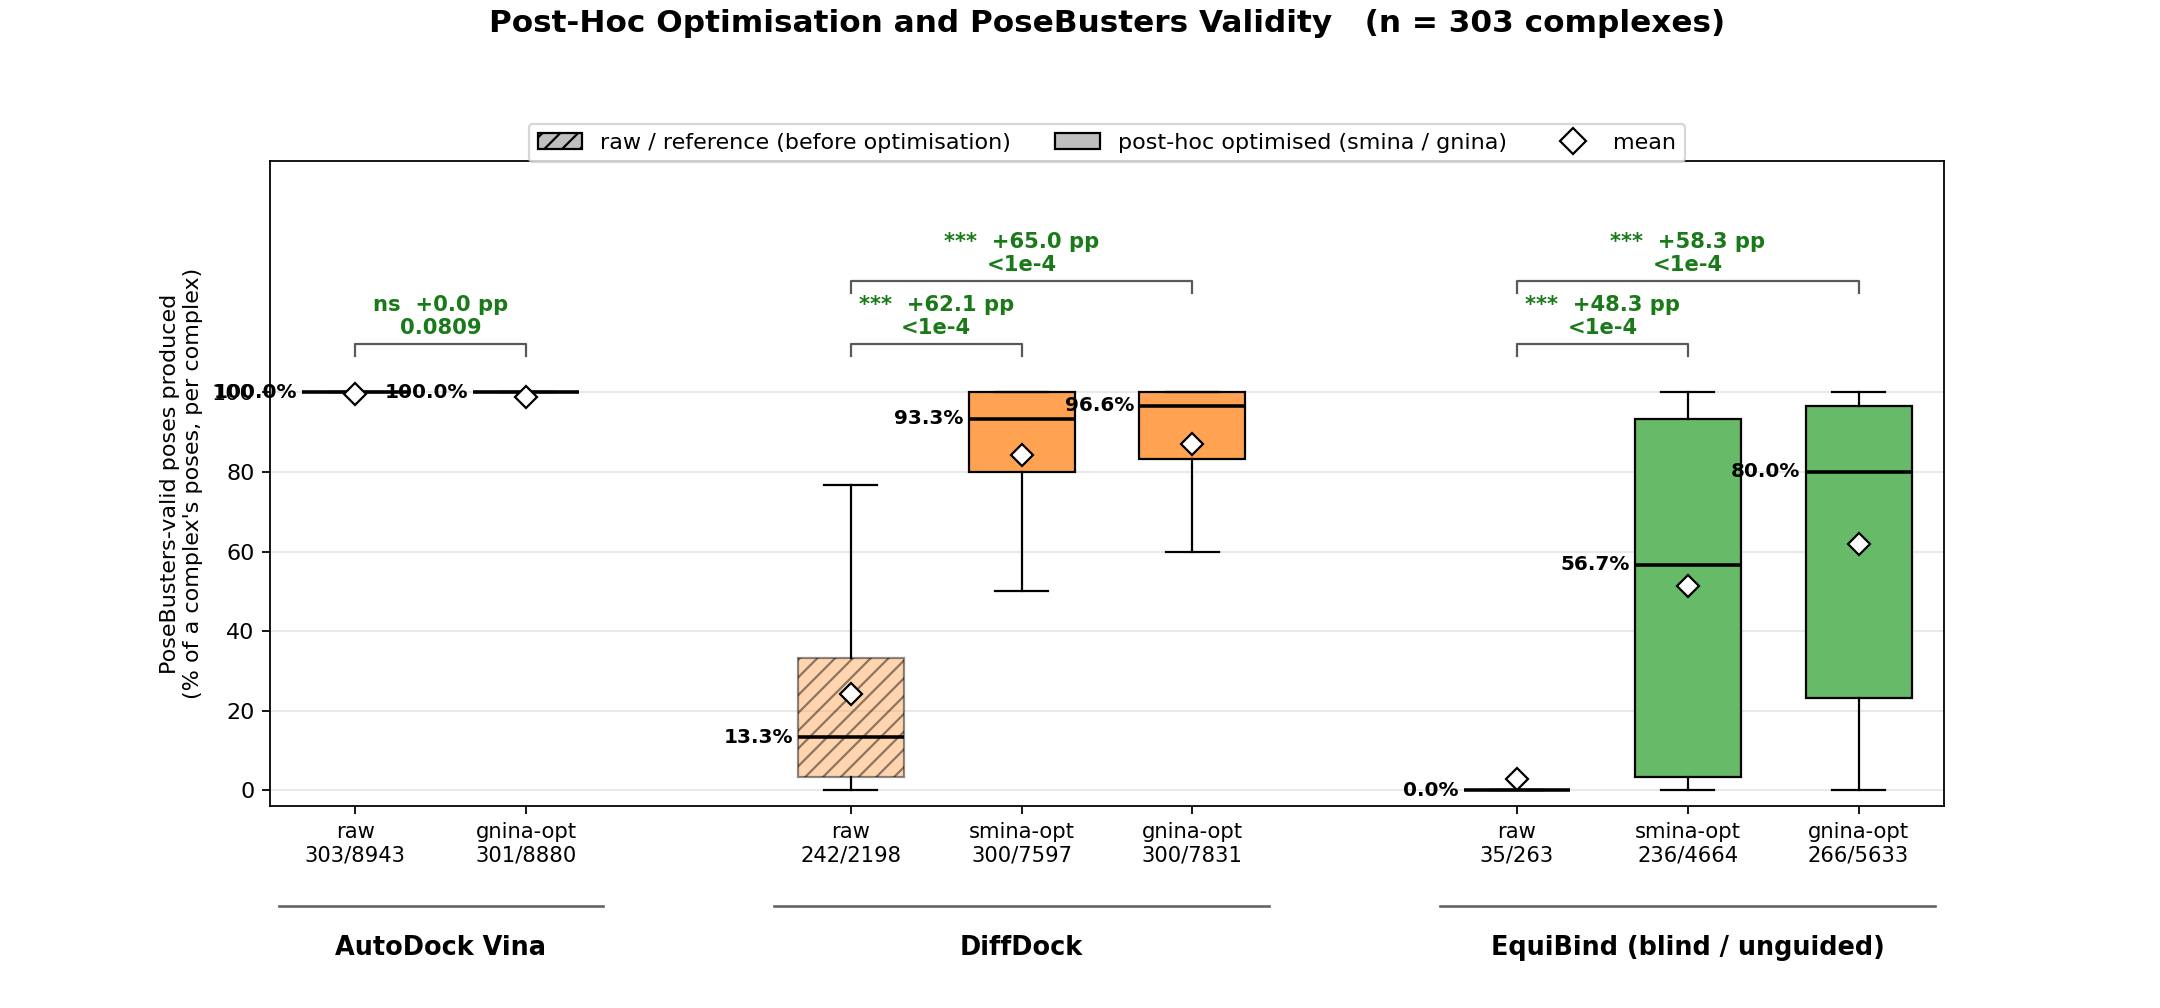
\includegraphics[width=\linewidth,height=0.78\textheight,keepaspectratio]{media/media/image2.png}
\caption{Post-hoc optimisation and PoseBusters validity. Significance brackets carry Holm-corrected p-values}\label{fig:results-r1}
\end{figure}

Figure~\ref{fig:results-r1} reports per-complex PoseBusters-validity yields before and after local optimisation. AutoDock's raw search is already almost perfectly valid. The median per-complex yield is 100\%, pooled validity is 99.6\%, and every one of the 303 complexes has at least one valid pose. Only 33 of 8,976 raw poses fail PoseBusters checks, split across internal clash (12), minimum distance to protein (20) and internal energy (1). Gnina rescoring leaves the median at 100\% and moves pooled validity to 98.9\%. The Hodges-Lehmann difference is exactly zero percentage points because 293 of the 303 complexes are unchanged, and the small movement that exists runs against rescoring (Wilcoxon p = 0.081). The two arms are level on physical validity with no headroom for an optimiser to repair.
DiffDock rises from a 13.3\% raw median to 93.3\% with smina, a Hodges-Lehmann gain of +62.1 percentage points. Unguided EquiBind rises from 0\% to 80.0\% with gnina. These near-unanimous gains survive Holm correction, with matched-pairs rank-biserial effects of 0.994--1.000 and adjusted p-values below 10\textsuperscript{-35}. DiffDock behaves similarly with gnina (96.6\%), whereas EquiBind performs worse with smina (56.7\%). The refiners are thus nearly interchangeable for DiffDock, while gnina is decisive for EquiBind.

% Removes since not relevant to the current discussion of PoseBusters validity.
% The hydrogen-handling artefact that inflates a raw-against-rescored validity comparison elsewhere does not arise here. Poses from the ADFRsuite-prepared arm carry no embedded SMILES, so both the raw and the rescored pose are rebuilt from a bond-order template as a heavy-atom record and PoseBusters adds and relaxes the whole hydrogen shell itself on each side. The added-hydrogen flag is set on 100\% of raw and 99.7\% of rescored poses, so the two arms are measured on the same footing and the comparison is a like-for-like one. What small movement there is runs against rescoring rather than for it, and it is concentrated rather than distributed. Rescoring raises internal-energy failures from 1 pose to 70 and leaves the intermolecular checks essentially unchanged, and 60 of the 63 additional invalid poses come from two complexes, 7NUT\_GLP and 7OZC\_G6S, which lose all thirty poses having been fully valid raw. The remaining 301 complexes still hold a valid rescored pose. Rescoring is therefore adopted for what it does to ranking, not to geometry, and the near-nativeness results below are where it earns its place. By contrast, minimisation makes most learned output physically valid.

Table~\ref{tab:appendix-pb-decomposition-full} in Appendix~\ref{supplementary-statistics} decomposes PoseBusters failure rates into the three groups. None of 72,219 poses from the eight reported variants fails a chemical-validity check. While only 25 poses fail bond length and 22 bond angle, most discrimination is intermolecular. Raw DiffDock has a 75.2\% intermolecular-failure rate against 75.6\% invalid overall, and raw EquiBind 96.8\% against 97.1\%. Minimum distance to protein dominates, failing 73.8\% of raw DiffDock and 96.5\% of raw EquiBind poses, compared with 0.2\% for AutoDock. Intramolecular failures matter only for raw EquiBind (27.9\%, versus at most 3.8\% for any AutoDock or DiffDock variant). A Benjamini-Hochberg analysis of the sixteen varying checks retains thirteen at q \textless{} 0.05, with minimum distance strongest (cp. Appendix~\ref{supplementary-statistics} for full analysis). Conditioning on poses already within 2\angstrom{} of the crystal indicates that placement, not chemistry, explains most of the remaining gap. The validity requirement removes at most four of 303 complexes from the headline endpoint at any depth. Appendix~\ref{validity-objective-coupling} reports both quantities and the overlap between intermolecular checks and the coordinate optimised by the search objective.

Table~\ref{tab:results-depth-recovery} compares rank-1, best-of-top-15 and best-of-top-30 pools. A complex is recovered if any inspected pose is PoseBusters-valid and within 2\angstrom{}. Because these pools are nested, deeper inspection can only add recoveries. All discordant pairs within a depth step therefore point in one direction, making recovery shares and confidence intervals more informative than a two-directional test. That test retains its usual interpretation between tools. Appendix~\ref{supplementary-statistics} gives the procedure.

\begin{longtable}[]{@{}
  >{\raggedright\arraybackslash}p{(\columnwidth - 10\tabcolsep) * \real{0.1156}}
  >{\raggedleft\arraybackslash}p{(\columnwidth - 10\tabcolsep) * \real{0.1573}}
  >{\raggedleft\arraybackslash}p{(\columnwidth - 10\tabcolsep) * \real{0.1573}}
  >{\raggedleft\arraybackslash}p{(\columnwidth - 10\tabcolsep) * \real{0.1573}}
  >{\raggedleft\arraybackslash}p{(\columnwidth - 10\tabcolsep) * \real{0.2059}}
  >{\raggedleft\arraybackslash}p{(\columnwidth - 10\tabcolsep) * \real{0.2065}}@{}}
\caption{PoseBusters Pass-All Recovery by Ranking Depth}\label{tab:results-depth-recovery}\tabularnewline
\toprule\noalign{}
{\raggedright \textbf{Method}} & \centering\arraybackslash\textbf{Rank-1} & \centering\arraybackslash\textbf{Best of top-15} & \centering\arraybackslash\textbf{Best of top-30} & \centering\arraybackslash\textbf{top-1\ensuremath{\rightarrow}15 gain} & \centering\arraybackslash\textbf{top-15\ensuremath{\rightarrow}30 gain} \\
\midrule\noalign{}
\endfirsthead
\caption[]{PoseBusters Pass-All Recovery by Ranking Depth (continued)}\tabularnewline
\toprule\noalign{}
{\raggedright \textbf{Method}} & \centering\arraybackslash\textbf{Rank-1} & \centering\arraybackslash\textbf{Best of top-15} & \centering\arraybackslash\textbf{Best of top-30} & \centering\arraybackslash\textbf{top-1\ensuremath{\rightarrow}15 gain} & \centering\arraybackslash\textbf{top-15\ensuremath{\rightarrow}30 gain} \\
\midrule\noalign{}
\endhead
\bottomrule\noalign{}
\endlastfoot
{\raggedright AutoDock} & {\raggedright 36.6\% (111)} & {\raggedright 65.3\% (198)} & {\raggedright 65.7\% (199)} & {\raggedright +87 (+28.7\%) ***} & {\raggedright +1 (+0.3\%)} \\
DiffDock & 34.0\% (103) & 55.1\% (167) & 55.8\% (169) & +64 (+21.1\%) *** & +2 (+0.7\%) \\
EquiBind & 18.2\% (55) & 26.4\% (80) & 26.4\% (80) & +25 (+8.3\%) *** & +0 (+0.0\%) \\
\multicolumn{6}{@{}p{\dimexpr\columnwidth-6\tabcolsep\relax}@{}}{\footnotesize%
Two-sided McNemar tests with Holm-Bonferroni correction, *** p \textless{} 0.001, ** p \textless{} 0.01 and * p \textless{} 0.05} \\
\multicolumn{6}{@{}p{\dimexpr\columnwidth-6\tabcolsep\relax}@{}}{\footnotesize%
Recovery is the PoseBusters-valid, within-2\angstrom{} recovery also reported across distance thresholds in Table~\ref{tab:results-near-native-form}, and the two coincide at every depth shown here.} \\
\end{longtable}
% UPDATED 2026-08-29 for the MGLTools/ADFRsuite exh128 arm; same existence gate as before
% (any pose in top-d that is PB-valid AND RMSD<=2A). Counts from
% benchmark_matched_equibind/.../per_pose_metrics.csv, DOMINANT AutoDock arm
% (REPOINTED 2026-09-01 from the superseded benchmark_full_protein_vina_scoring tree.)
% autodock_mgltools_exh128_gnina: 111/198/199 (the raw exh128 arm is 94/185/202 and must NOT be
% used to regenerate this table). Superseded Meeko figures were 89/151/151.
% OLD NOTE, kept for provenance:
% DiffDock-smina 103/167/169, EquiBind-gnina 55/80/80 (--minimize arm, re-derived 2026-09-01;
% the superseded --local_only arm read 46/61/62 and must NOT be used).
% Depth-gain decomposition (appendix tab:results-depth-gain), same gnina/smina arm, re-derived
% 2026-09-01 from benchmark_matched_equibind: near-native gained +88/+63/+26; of which remain
% PB-invalid -2/-1/-2; valid rescued +1/+2/+1; net +87/+64/+25, matching this table's gain column.
% 15->30 gains on the PRINTED gnina/smina arm (autodock_gnina by optimized_rank, diffdock_smina,
% equibind_unguided_gnina by gnina_affinity): discordant b = 0/2/1, c = 0 throughout, exact two-sided
% p = 1.0/0.5/1.0, none significant (no stars). Counts 198->199, 167->169, 80->80,
% discordant b = 1/2/0, c = 0 throughout (re-derived 2026-09-01 on the --minimize arm).
% (An earlier note here recorded b=5 -> p=0.0625; that is the RAW Vina arm 145->150, which the lines
%  above forbid for this table. Re-derived 2026-08-16 from per_pose_metrics.csv.)

Table~\ref{tab:results-depth-gain} in Appendix~\ref{supplementary-statistics} decomposes the reservoir of lower-ranked PoseBusters-valid poses in greater detail. 


\hypertarget{near-nativeness-and-form}{%
\subsection{Near-Nativeness and Form}\label{near-nativeness-and-form}}

Figures~\ref{fig:results-r2a} and \ref{fig:results-r2b} report accuracy for the 303 complexes with PoseBusters-valid poses against as-placed crystal RMSD (i.e. near-nativeness) and best-fit Kabsch RMSD (i.e. form), separating placement from form. The vertical axis gives the percentage of complexes with at least one valid pose within the distance threshold among the first d ranks. Differences among the top-1, top-15 and top-30 curves measure ranking headroom \footnote{Table~\ref{tab:results-near-native-form} in Appendix~\ref{supplementary-statistics} provides ten distance thresholds.}, namely valid near-native poses generated but ranked below d, distinguishing sampling from scoring \cite{ref050}, \cite{ref052}. 

Near-native recovery differs among tools at every depth (Cochran\textquotesingle s Q p \textless{} 1e-7). At 2\angstrom{}, AutoDock has the highest point estimate with margins over DiffDock opening at top-5 and narrowing slightly with increasing depth. Rank-1 accuracy is 36.6\% for AutoDock, 34.0\% for DiffDock and 18.2\% for EquiBind. AutoDock and DiffDock exceed EquiBind at every depth (all p\_holm \textless{} 3e-7). AutoDock and DiffDock do not differ detectably at rank-1, where the gap is +2.6 percentage points (Newcombe hybrid-score 95\% interval \ensuremath{-}4.2 to +9.4, exact McNemar p = 0.509), but they do from top-5 onwards, by +13.2 points at top-5 (+5.7 to +20.4, p\_holm = 7.6e-4), +10.2 at top-15 (+2.8 to +17.5, p\_holm = 0.009) and +9.9 at top-30 (+2.5 to +17.1, p\_holm = 0.011). Thus, ordering is a statement about the pool inspected rather than about a single nominated pose, where the two tools remain indistinguishable. 

However, AutoDock's lead is attributed to fine-tuning exhaustiveness (cp. Appendix~\ref{exhaustiveness-selection}) whereas DiffDock and EquiBind arms enhancement was based on post-hoc refinement solely. The head-to-head comparison sets a tuned pipeline against two untuned ones, and the AutoDock figures carry a rank-1 selection optimism that the other two do not, quantified in the same appendix. What the ordering establishes is narrower than a comparison of method classes. The carried-forward AutoDock arm is itself CNN-rescored by gnina. The contrast is therefore between two configured workflows on this benchmark and not between physics-based and AI-based docking.

The rank-1 contrast draws information only from the 112 discordant complexes, so the minimum detectable difference there is 9.8 percentage points at 80\% power and the study is underpowered for the observed +2.6-point estimate. No equivalence margin was prespecified, and the non-significant rank-1 result does not establish equivalence. Appendix~\ref{supplementary-statistics} gives the power calculation and projected sample size.

Ranking depth affects every tool (Cochran\textquotesingle s Q p \textless{} 1e-6 throughout). From rank-1 to best-of-top-15, AutoDock gains +28.7 percentage points (Wilson 95\% interval 23.9--34.0), DiffDock +21.1 (16.9--26.1) and EquiBind +8.3 (5.7--11.9). AutoDock rises from 36.6\% to 65.3\%, adding 87 complexes compared with DiffDock\textquotesingle s 64. The selection gaps align with the sampling and scoring distinction \cite{ref003}, \cite{ref050}, \cite{ref052} and with the gap DiffDock reports between its top-ranked pose and its wider sample \cite{ref024}. Rescoring with gnina captures part of that headroom prospectively rather than retrospectively, raising AutoDock\textquotesingle s rank-1 recovery from 31.0\% to 36.6\% and its top-15 recovery from 61.1\% to 65.3\%. Since that pass reorders the pool rather than enlarging it, the gain is confined to the top of the list. Over the whole pool the raw search is nominally ahead, 202 complexes against 199, because rescoring minimises every pose and a few cross the threshold the wrong way (Appendix~\ref{exhaustiveness-selection}). EquiBind\textquotesingle s smaller gain indicates a sampling constraint. A single-shot regression model provides few distinct alternatives, and rescoring cannot recover poses that were not generated.

\begin{figure}[!htbp]
\centering
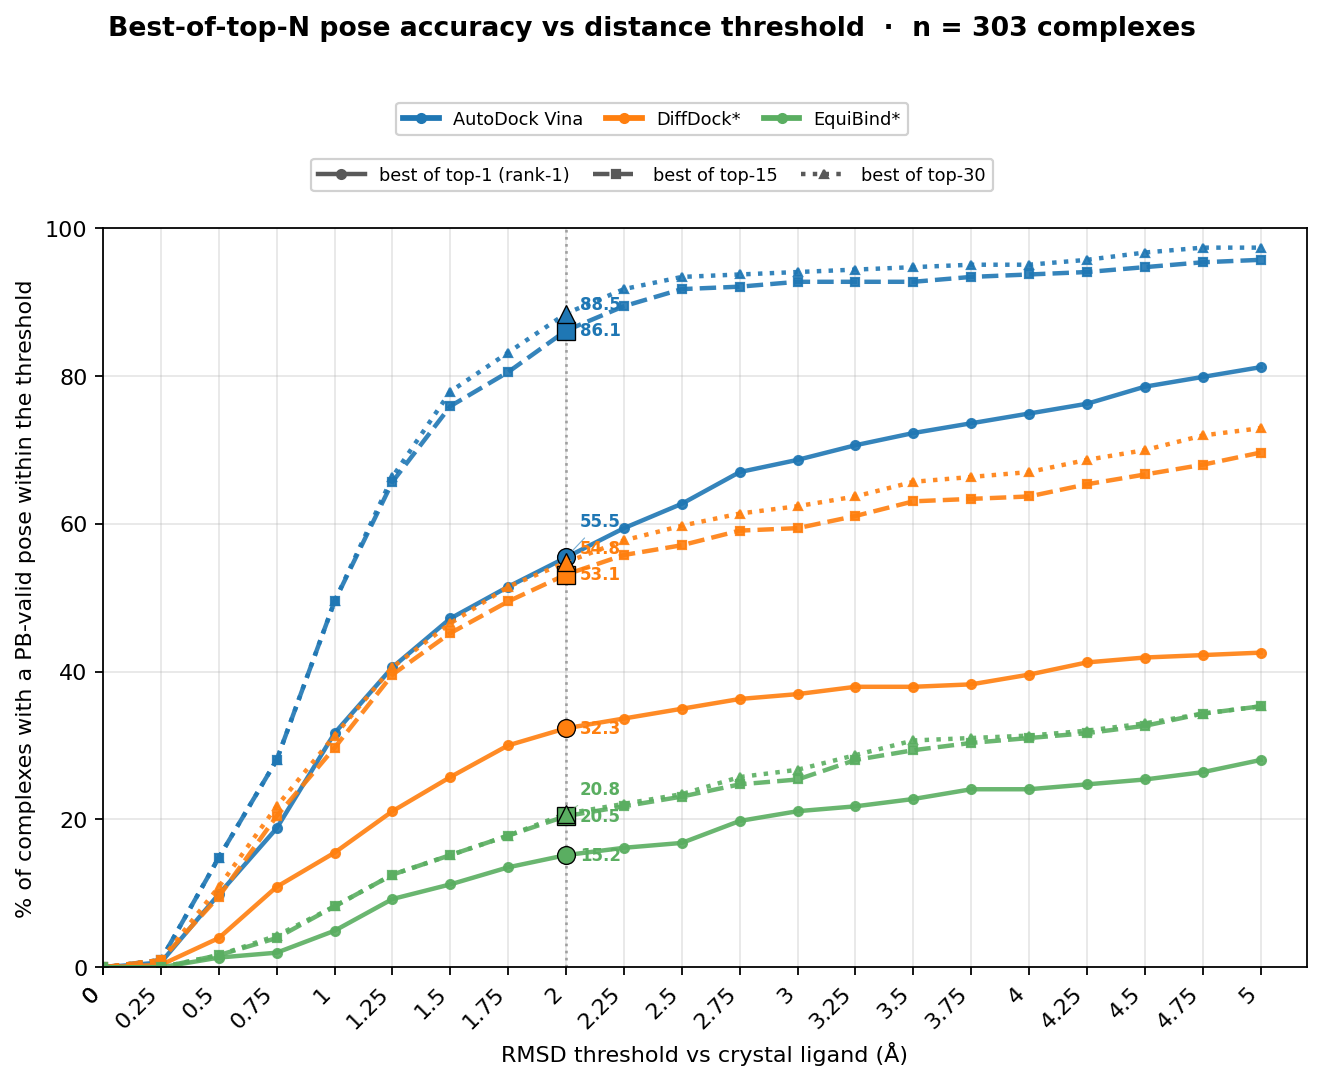
\includegraphics[width=0.86\linewidth,height=0.78\textheight,keepaspectratio]{media/media/image3.png}
\caption{Best-of-top-N accuracy against the as-placed crystal RMSD}\label{fig:results-r2a}
\end{figure}

Kabsch RMSD isolates ligand form. AutoDock and DiffDock recover 74.3\% and 74.6\%, respectively, at the primary 1\angstrom{} threshold and best-of-top-30 depth, compared with 95.4\% and 97.0\% at 2\angstrom{}. Form differs among tools at every depth (Cochran\textquotesingle s Q p \textless{} 1e-9). Rank-1 recovery is 52.5\% for AutoDock, 52.1\% for DiffDock and 33.3\% for EquiBind. AutoDock and DiffDock exceed EquiBind at every depth (p\_holm \ensuremath{\leq} 4e-10). In contrast, the AutoDock--DiffDock comparison is a tie throughout, at p\_holm = 1.000 with 47 against 46 discordant complexes at rank-1, 30 against 31 at top-15 and 25 against 26 at top-30. Form is the one axis on which a physics-based search and a diffusion model are statistically indistinguishable. No equivalence margin was prespecified. This is an absence of detected difference rather than a demonstration of equivalence. DiffDock generates the right shape and localises it less well, consistent with its generative treatment of torsional, rotational and translational degrees of freedom \cite{ref024}. AutoDock samples rigid-receptor placements whose internal geometry is constrained by construction.

\begin{figure}[!htbp]
\centering

\includegraphics[width=0.86\linewidth,height=0.78\textheight,keepaspectratio]{media/media/image4.png}
\caption{Best-of-top-N accuracy against the best-fit (Kabsch) RMSD}\label{fig:results-r2b}
\end{figure}

EquiBind remains weakest on form, rising from 33.3\% at rank-1 to 54.1\% at best-of-top-30. This indicates internal-geometry error in addition to misplacement and agrees with evaluations in which direct regression trails diffusion and hybrid methods on combined geometry and validity \cite{ref013}, \cite{ref035}. The 20.8-point depth gain provides evidence of acceptable but mislocated shape poses. From top-15 to top-30, placement gains at most 0.7 points, whereas form at 1\angstrom{} gains 2.3 points for both AutoDock and DiffDock and 3.0 for EquiBind (Table~\ref{tab:results-near-native-form}).

The near-nativeness and form endpoints separate the tools differently. On placement AutoDock leads from top-5 onwards. On form AutoDock and DiffDock are indistinguishable everywhere. On pooled physical validity AutoDock leads throughout, at 98.9\% against 84.5\% for DiffDock. Their top-15 selection gains are 87 and 64 complexes, yet about six in ten rank-1 failures contain no qualifying pose anywhere in the pool. Generation and localisation therefore remain the larger constraints \cite{ref003}, \cite{ref013}, \cite{ref024}, \cite{ref035}. Refined-score ordering can be considered an unclaimed remedy for DiffDock, worth about three points of rank-1 recovery on the reported coordinates. For AutoDock a larger sampling budget was tested directly (cp. Appendix~\ref{exhaustiveness-selection}).

Figure~\ref{fig:results-r3} plots in-place against Kabsch RMSD, separating placement-limited, form-limited and mixed errors. Its columns expand the pool from rank-1 to best-of-top-5 and best-of-top-15. Arrows trace each cohort median from rank-1. Table~\ref{tab:results-placement-form} in Appendix~\ref{supplementary-statistics} provides details about the distributions.\footnote{Poses whose docked centroid lies more than 8\angstrom{} from the crystal-ligand site were removed leaving 6,169 PoseBusters-valid poses for scoring. Axes are clipped at 5\angstrom{} keeping dense near-native core legible, yet removing 2,329 poses from the graph frame.}

AutoDock returns a valid pose for all 303 complexes, but only 62.7\% remain after the rank-1 crystal-site trim. Its median in-place RMSD deteriorates most with depth, from 1.5\angstrom{} at rank-1 to 5.0\angstrom{} at top-15. The +3.55\angstrom{} shift has a receptor-bootstrap interval of +3.00 to +3.99\angstrom{} and is supported across disjoint within-complex rank bands (Friedman p \textless{} 1e-15). Placement-limited poses rise from 48\% to 78\%, while form-limited poses fall from 27\% to 8\%. Deeper ranks therefore add mainly correctly shaped but misplaced ligands, consistent with the largest within-complex spread (5.72\angstrom{}). Ranking is informative only near the top.

DiffDock is most stable with depth in the near-site cohort, drifting +0.46\angstrom{} in place versus +3.55\angstrom{} for AutoDock and +1.09\angstrom{} for EquiBind. Expanding the pool fifteen-fold keeps DiffDock medians near 1.5--1.9\angstrom{} in place and 0.9\angstrom{} in form. It is significantly best on both axes at top-5 and top-15. Form shifts only +0.03\angstrom{} (bootstrap interval \ensuremath{-}0.05 to +0.12\angstrom{}), although disjoint rank bands differ across the 137 complete complexes (Friedman p = 0.006). This statistically detected but negligible change partly reflects low diversity. DiffDock\textquotesingle s within-complex spread is 2.34\angstrom{}, compared with 5.72\angstrom{} for AutoDock.

EquiBind produces at least one valid pose for 266 of 303 complexes, but valid-near-native recovery is only 26.4\% by top-15 and 26.4\% over all thirty poses. Its rank-1 median in-place RMSD of 2.9\angstrom{} already exceeds the near-native threshold. Gnina minimisation repairs some local defects but not gross localisation failures.

\begin{figure}[!htbp]
\centering

\includegraphics[width=0.86\linewidth,height=0.78\textheight,keepaspectratio]{media/media/image5.png}
\caption{Form versus in-place RMSD across ranking depth}\label{fig:results-r3}
\end{figure}

In the near-site cohort, deeper ranks add valid but misplaced AutoDock and EquiBind poses and few for DiffDock. In-place RMSD deteriorates with depth. DiffDock appears more form-limited only because its low in-place RMSD inflates the form-to-in-place ratio. Its absolute form RMSD is lowest.

\hypertarget{cross-tool-clustering}{%
\subsection{Cross-Tool Clustering}\label{cross-tool-clustering}}

Poses from the three selected variants were pooled without validity filtering, clustered and scored for crystal-site recovery under the 4\angstrom{} rule defined in the Methods. Sixteen of 303 complexes have no qualifying cluster and count as non-reaches. Figure~\ref{fig:results-r4} and Table~\ref{tab:results-cluster-recovery} report top-N recovery for individual tools and combinations.

\begin{figure}[!htbp]
\centering

\includegraphics[width=\linewidth,height=0.78\textheight,keepaspectratio]{media/media/image6.png}
\caption{Top-N crystal-cluster co-recovery}\label{fig:results-r4}
\end{figure}

AutoDock and DiffDock have almost fully overlapping reach intervals at every depth, while EquiBind trails both. From rank-1 to top-15, DiffDock gains 26 percentage points, AutoDock 24 and EquiBind 4. Pairings become less redundant with depth but remain positively associated. At top-15, all converge at \ensuremath{\phi} = +0.23 to +0.28 with Fisher p \ensuremath{\leq} 2.8e-4.

\begin{longtable}[]{@{}
  >{\raggedright\arraybackslash}p{(\columnwidth - 8\tabcolsep) * \real{0.4200}}
  >{\centering\arraybackslash}p{(\columnwidth - 8\tabcolsep) * \real{0.1450}}
  >{\centering\arraybackslash}p{(\columnwidth - 8\tabcolsep) * \real{0.1450}}
  >{\centering\arraybackslash}p{(\columnwidth - 8\tabcolsep) * \real{0.1450}}
  >{\centering\arraybackslash}p{(\columnwidth - 8\tabcolsep) * \real{0.1450}}@{}}
\caption{Crystal-Cluster Reach and Co-Reach by Ranking Depth}\label{tab:results-cluster-recovery}\tabularnewline
\toprule\noalign{}
{\raggedright \textbf{Statistic}} & \centering\arraybackslash\textbf{top-1} & \centering\arraybackslash\textbf{top-5} & \centering\arraybackslash\textbf{top-10} & \centering\arraybackslash\textbf{top-15} \\
\midrule\noalign{}
\endfirsthead
\caption[]{Crystal-Cluster Reach and Co-Reach by Ranking Depth (continued)}\tabularnewline
\toprule\noalign{}
{\raggedright \textbf{Statistic}} & \centering\arraybackslash\textbf{top-1} & \centering\arraybackslash\textbf{top-5} & \centering\arraybackslash\textbf{top-10} & \centering\arraybackslash\textbf{top-15} \\
\midrule\noalign{}
\endhead
\bottomrule\noalign{}
\endlastfoot
AutoDock reach \% {[}95\% CI{]} & 59 {[}53--64{]} & 79 {[}74--83{]} & 81 {[}76--85{]} & 83 {[}79--87{]} \\
DiffDock reach \% {[}95\% CI{]} & 54 {[}49--60{]} & 76 {[}70--80{]} & 79 {[}74--83{]} & 81 {[}76--85{]} \\
EquiBind reach \% {[}95\% CI{]} & 43 {[}37--49{]} & 46 {[}40--51{]} & 47 {[}41--52{]} & 47 {[}42--53{]} \\
AutoDock + DiffDock co-reach\footnote{Co-reach \ensuremath{\phi} is the signed association between two tools\textquotesingle{} per-complex reach against independence, where a positive value means the pair succeeds and fails together. All three pairings reach p \textless{} 0.05 on a two-sided Fisher test. Three-way agreement exceeds chance at every depth with a permutation p below 1e-4, and the ranking depths are nested cumulative thresholds rather than an independent test family.} \ensuremath{\phi} & \textbf{+0.33} & \textbf{+0.23} & \textbf{+0.24} & \textbf{+0.23} \\
AutoDock + EquiBind co-reach \ensuremath{\phi} & \textbf{+0.45} & \textbf{+0.27} & \textbf{+0.29} & \textbf{+0.28} \\
DiffDock + EquiBind co-reach \ensuremath{\phi} & \textbf{+0.42} & \textbf{+0.30} & \textbf{+0.29} & \textbf{+0.26} \\
All three reach, complexes observed / expected & 89 / 42 & 114 / 82 & 121 / 90 & 125 / 96 \\
\multicolumn{5}{@{}p{\dimexpr\columnwidth-5\tabcolsep\relax}@{}}{\footnotesize%
The three reach rows are percentages of the 303 complexes, carried with Wilson 95\% intervals.} \\
\end{longtable}

\begin{figure}[!htbp]
\centering
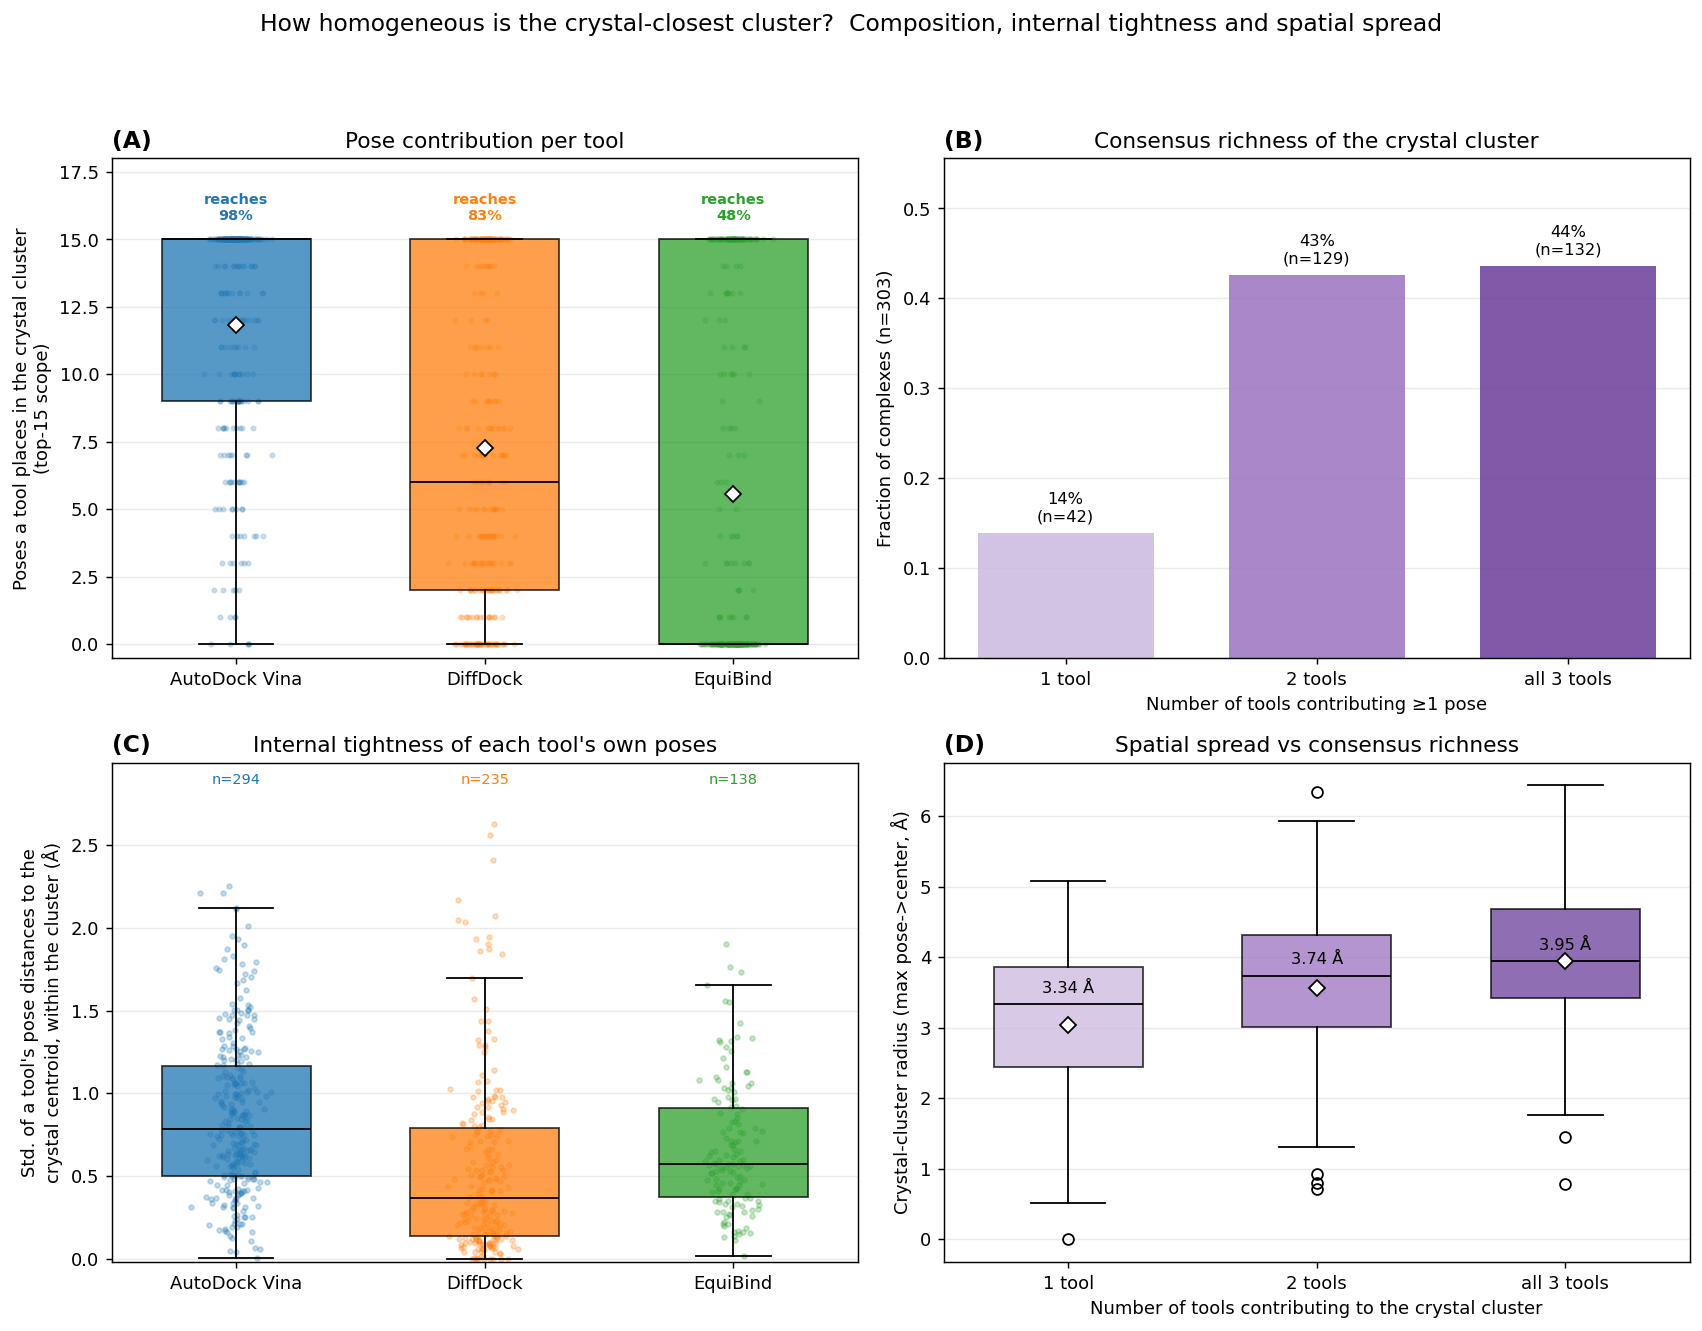
\includegraphics[width=\linewidth,height=0.78\textheight,keepaspectratio]{media/media/image7.png}
\caption{Composition and geometry of the crystal-closest cluster. Rates are taken over all 303 complexes, 18 of which contribute no pose to any panel}\label{fig:results-r5}
\end{figure}

Figure~\ref{fig:results-r5} (A) gives DiffDock a median six of fifteen poses in the crystal cluster and 81\% reach, and AutoDock five poses and 83\% reach. EquiBind has a median of zero and 47\% reach. In the reported top-15 analysis the two leading tools differ in pose count, where DiffDock contributes more (Holm-corrected rank-biserial \ensuremath{-}0.28, p = 2.7e-4), but not in reach (McNemar p = 0.470 on 38 against 31 discordant complexes). Both exceed EquiBind on reach. Panel (B) shows polarised consensus, with 125 complexes solved by all tools versus 96.1 expected (permutation p \textless{} 1e-4), and 18 by none versus 5.2 expected. AutoDock accounts for 28 of the 55 single-tool solutions, compared with 25 for DiffDock and two for EquiBind. Panel (C) plots, for each complex and tool, the standard deviation of that tool\textquotesingle s in-cluster poses in their distance to the crystal centroid. The median is 0.70\angstrom{} for AutoDock over 233 defined complexes, 0.56\angstrom{} for EquiBind over 135 and 0.38\angstrom{} for DiffDock over 229. Cohorts differ because the statistic requires at least two within-cluster poses, making missingness informative. The measure is radial, and poses lying at a common distance from the crystal centroid can still sit far apart. A large value therefore establishes real spatial spread, whereas a small value does not establish that a tool\textquotesingle s poses sit together. The supported reading is that AutoDock scatters its in-cluster poses along the radial coordinate. A paired restriction to the 110 complexes defined for all tools keeps AutoDock highest on this statistic, at 0.70\angstrom{} against 0.57\angstrom{} and 0.31\angstrom{}. Appendix~\ref{supplementary-statistics} gives the omnibus and pairwise statistics.

Panel (D) shows median cluster radius increasing from 2.13\angstrom{} for single-tool clusters to 3.72\angstrom{} for three-tool clusters, but the association is no longer detectable after adjustment for pose count (partial \ensuremath{\rho} = \ensuremath{-}0.07, p = 0.26). The partition has a median bootstrap Jaccard of 0.78. At the 4\angstrom{} crystal-site threshold, the retrospective oracle recovers 95\% of complexes, compared with about 56\% for the best inexpensive first-cluster rules. Consensus ranking reaches 56.8\%, its medoid-centred variant 55.4\% and confidence weighting 55.8\%. These three rules are not separable from one another, and they gain 7.3, 5.9 and 6.3 points respectively on the 49.5\% legacy pose-count rule. All three clear correction against it (Holm-corrected McNemar p = 3.6e-4 for consensus ranking, 0.004 for confidence weighting and 0.008 for its medoid-centred variant). The 38-point oracle gap reflects site ranking. The pooled cloud usually contains the crystal-compatible region, but blind prospective selection remains difficult. Figure~\ref{fig:results-r6} in Appendix~\ref{supplementary-statistics} reports internal validity, resampling stability and precision-at-one for all five rules.

Across the full pose cloud, the pooled three-tool oracle places a pose within 4\angstrom{} of the crystal site for 97.7\% of complexes, at a median distance of 0.34\angstrom{}. AutoDock alone reaches 88.1\% at 0.53\angstrom{} and DiffDock 84.5\% at 0.56\angstrom{}. Together they already reach 97.7\% at 0.37\angstrom{}, so EquiBind adds nothing to the pooled reach. Averaging cluster members makes the pooled centre coarser than the best individual pose, with a median distance of 1.23\angstrom{}.

\hypertarget{interaction-and-contact-analysis}{%
\subsection{Interaction and Contact Analysis}\label{interaction-and-contact-analysis}}

Crystal-pose interactions are compared with those of PoseBusters-valid pipeline poses. PandaMap detects typed contacts \cite{ref090} using PLIP-style categories \cite{ref054} but only distance and atom-type criteria in this execution path. Because fingerprints encode residue identity, all poses and the crystal reference use one common author-numbered receptor per complex (Appendix~\ref{interaction-fingerprints}). Figure~\ref{fig:results-r7} gives mean Jaccard overlap for each tool\textquotesingle s top-5 union. Each cell averages the complexes for which both entries are defined, not one matrix-wide cohort.

\begin{figure}[!htbp]
\centering

\includegraphics[width=\linewidth,height=0.78\textheight,keepaspectratio]{media/media/image9.png}
\caption{Mean Jaccard similarity of interaction fingerprints, whole-protein search}\label{fig:results-r7}
\end{figure}

DiffDock has the highest mean typed-interaction Jaccard similarity to the crystal, at 0.450 over 300 complexes, compared with 0.417 over 301 for AutoDock and 0.380 over 266 for EquiBind. That ordering survives restriction to a common cohort. Across the 264 complexes defined for all tools, DiffDock reaches 0.474, AutoDock 0.431 and EquiBind 0.381. DiffDock leads AutoDock (Wilcoxon p = 0.014) and both exceed EquiBind (p = 1.6e-3 and 5.2e-8). AutoDock averages only 0.313 on the 37 complexes lacking a valid EquiBind pose. Pairwise tool similarities range from 0.357 to 0.463, and the AutoDock--DiffDock pair at 0.463 exceeds either tool\textquotesingle s similarity to the crystal. The two therefore resemble each other more than either resembles the reference and thus have different contact hypotheses. Because Jaccard counts both shared and non-shared interactions, it is not contact recall.

Table~\ref{tab:results-native-recovery-rank} reports precision, recall and F1 by each tool\textquotesingle s own rank k among all produced poses, profiling only PoseBusters-valid poses. AutoDock uses gnina re-ranking, EquiBind gnina affinity and DiffDock native confidence retained through smina refinement. A failed top-ranked pose contributes no k = 1 value, affecting 5 of 303 AutoDock complexes and 21 of the 303 with DiffDock output. EquiBind ranks only retained valid poses and therefore always begins at k = 1.

Rank-1 F1 is 0.57 for AutoDock, 0.53 for DiffDock and 0.47 for EquiBind, but these means use different available-case cohorts and were not tested for equivalence. Across 280 shared AutoDock--DiffDock complexes, the means are 0.5663 and 0.5324 without a detected difference (Wilcoxon p = 0.25). Scoring a missing valid rank-1 pose as zero across all 303 complexes preserves the order and widens it, to 0.556 for AutoDock and 0.492 for DiffDock, which more often lacks a valid nominee. Rank-1 contact fidelity is therefore conditional on a valid top pose, though the ordering here is not sensitive to how missing poses are treated. By rank 5, AutoDock declines to 0.42, while DiffDock remains near 0.51 and EquiBind near 0.44. DiffDock consequently leads for the top-5 union in Figure~\ref{fig:results-r7} without leading on the nominated pose. Per-complex Kendall \ensuremath{\tau} links AutoDock rank to better poses. EquiBind gnina-affinity rank similarly orders recall and F1. DiffDock confidence has no detected association with interaction recovery, so its top pose cannot be expected from these data to outperform rank 5. This is absence of detected ordering, not proof that confidence lacks signal. Appendix~\ref{supplementary-statistics} gives the nine BH-corrected \ensuremath{\tau} tests.

\begin{longtable}[]{@{}
  >{\raggedright\arraybackslash}p{(\columnwidth - 10\tabcolsep) * \real{0.3000}}
  >{\centering\arraybackslash}p{(\columnwidth - 10\tabcolsep) * \real{0.1400}}
  >{\centering\arraybackslash}p{(\columnwidth - 10\tabcolsep) * \real{0.1400}}
  >{\centering\arraybackslash}p{(\columnwidth - 10\tabcolsep) * \real{0.1400}}
  >{\centering\arraybackslash}p{(\columnwidth - 10\tabcolsep) * \real{0.1400}}
  >{\centering\arraybackslash}p{(\columnwidth - 10\tabcolsep) * \real{0.1400}}@{}}
\caption{Native-Interaction Recovery versus the Crystal by Pose Rank, Whole-Protein Search}\label{tab:results-native-recovery-rank}\tabularnewline
\toprule\noalign{}
{\raggedright \textbf{Tool and statistic}} & \centering\arraybackslash\textbf{k = 1} & \centering\arraybackslash\textbf{k = 2} & \centering\arraybackslash\textbf{k = 3} & \centering\arraybackslash\textbf{k = 4} & \centering\arraybackslash\textbf{k = 5} \\
\midrule\noalign{}
\endfirsthead
\caption[]{Native-Interaction Recovery versus the Crystal by Pose Rank, Whole-Protein Search (continued)}\tabularnewline
\toprule\noalign{}
{\raggedright \textbf{Tool and statistic}} & \centering\arraybackslash\textbf{k = 1} & \centering\arraybackslash\textbf{k = 2} & \centering\arraybackslash\textbf{k = 3} & \centering\arraybackslash\textbf{k = 4} & \centering\arraybackslash\textbf{k = 5} \\
\midrule\noalign{}
\endhead
\bottomrule\noalign{}
\endlastfoot
AutoDock complexes n & 298 & 298 & 299 & 296 & 299 \\
AutoDock precision & 0.561 & 0.550 & 0.485 & 0.497 & 0.439 \\
AutoDock recall & 0.572 & 0.548 & 0.477 & 0.479 & 0.414 \\
AutoDock F1 & 0.565 & 0.546 & 0.479 & 0.485 & 0.423 \\
DiffDock complexes n & 282 & 267 & 277 & 270 & 275 \\
DiffDock precision & 0.536 & 0.529 & 0.520 & 0.497 & 0.528 \\
DiffDock recall & 0.526 & 0.511 & 0.496 & 0.471 & 0.504 \\
DiffDock F1 & 0.529 & 0.517 & 0.503 & 0.479 & 0.512 \\
EquiBind complexes n & 266 & 256 & 247 & 245 & 243 \\
EquiBind precision & 0.493 & 0.489 & 0.488 & 0.476 & 0.472 \\
EquiBind recall & 0.459 & 0.451 & 0.450 & 0.433 & 0.423 \\
EquiBind F1 & 0.471 & 0.465 & 0.463 & 0.449 & 0.441 \\
\multicolumn{6}{@{}p{\dimexpr\columnwidth-6\tabcolsep\relax}@{}}{\footnotesize%
Each cell is the unweighted mean over the complexes that contribute a PoseBusters-valid pose at that rank. The three tools are therefore compared on overlapping rather than identical cohorts.} \\
\end{longtable}

Figure~\ref{fig:results-r9} in Appendix~\ref{supplementary-statistics} decomposes these poses into matched, missed and spurious contacts. At rank 1, AutoDock and DiffDock recover 21.0 and 19.4 native contacts while missing 15.3 and 16.4. By rank 5, AutoDock falls to 15.3 matched against 21.0 missed, while spurious contacts rise to 17.6. It is the only pipeline whose spurious count increases significantly with rank. DiffDock remains near 18.6 matched and 17.4 missed with stable spurious counts. EquiBind misses more native contacts than it recovers at every rank, under-reproducing the native network while generating the fewest non-native contacts.

AutoDock and DiffDock show no detected difference in nominated rank-1 contact fidelity, but the result is inconclusive rather than equivalent. Gnina ranks AutoDock\textquotesingle s steeply declining series informatively, with all three per-complex Kendall correlations negative and surviving correction. DiffDock\textquotesingle s flatter pool remains unordered, and neither tested refined score improves it. EquiBind recovers few native contacts at any rank.

\protect\hypertarget{_Toc235735934}{}{}

\hypertarget{experimental-dataset-1}{%
\section{Experimental Dataset}\label{experimental-dataset-1}}

The experimental evaluation tests whether the ordering established against crystallographic references transfers to a pharmacologically relevant target. The Orai1 channel was docked with three functionally validated modulators, 2-APB, GSK-7975A and Synta-66. No ligand-bound Orai structure exists, and the receptor is an ensemble of molecular-dynamics snapshots. The Appendix (Docking Protocols, Orai1 Panels) specifies the settings and differences between the panels.

The experimental panel pairs three modulators with four Orai1 frames, providing twelve frame-ligand units. The control panel adapts the decoy-set practice of docking a large library of molecules, i.e. calibration dataset ligands, with no known target activity \cite{ref045}, \cite{ref046}, against which the compounds of interest are compared. The control panel is only a background comparator, and no enrichment claim is made. Of 1,232 possible combinations of 308 calibration ligands and four frames, AutoDock and EquiBind cover all 1,232 while DiffDock covers 1,215, i.e. the cross-tool comparisons rest on 1,215 units. Both panels use the selected calibration variant of each engine, namely AutoDock Vina + gnina, DiffDock + smina and EquiBind + gnina. Output is capped at the top ten ranked poses per unit, or the top three for interaction and contact analysis. DiffDock returned fewer than ten poses for 178 of its 1,215 units. Per-unit rates therefore use the poses produced, not a fixed denominator of ten. Appendix~\ref{orai1-panels} gives the per-frame drops and panel totals. Poses within a unit are correlated, and the twelve experimental units represent only three chemotypes and one receptor trajectory. Comparisons are therefore exploratory and emphasise effect sizes and uncertainty rather than p-values alone.

Table~\ref{tab:results-orai-yield} provides the end-to-end yield funnel, from produced poses through PoseBusters validity to the combined validity-and-placement endpoint.

\begin{longtable}[]{@{}
  >{\raggedright\arraybackslash}p{(\columnwidth - 12\tabcolsep) * \real{0.2140}}
  >{\raggedright\arraybackslash}p{(\columnwidth - 12\tabcolsep) * \real{0.1800}}
  >{\raggedleft\arraybackslash}p{(\columnwidth - 12\tabcolsep) * \real{0.1213}}
  >{\raggedleft\arraybackslash}p{(\columnwidth - 12\tabcolsep) * \real{0.1213}}
  >{\raggedleft\arraybackslash}p{(\columnwidth - 12\tabcolsep) * \real{0.1213}}
  >{\raggedleft\arraybackslash}p{(\columnwidth - 12\tabcolsep) * \real{0.1213}}
  >{\raggedleft\arraybackslash}p{(\columnwidth - 12\tabcolsep) * \real{0.1213}}@{}}
\caption{Physical-Validity and Operational-Placement Yield for the Orai1 Experimental Ligands}\label{tab:results-orai-yield}\tabularnewline
\toprule\noalign{}
{\raggedright Tool} & \centering\arraybackslash Ligand & \centering\arraybackslash Poses & \centering\arraybackslash PB-valid Poses & \centering\arraybackslash PB-valid \% & \centering\arraybackslash PB-valid usable & \centering\arraybackslash PB-valid usable \% \\
\midrule\noalign{}
\endfirsthead
\caption[]{Physical-Validity and Operational-Placement Yield for the Orai1 Experimental Ligands (continued)}\tabularnewline
\toprule\noalign{}
{\raggedright Tool} & \centering\arraybackslash Ligand & \centering\arraybackslash Poses & \centering\arraybackslash PB-valid Poses & \centering\arraybackslash PB-valid \% & \centering\arraybackslash PB-valid usable & \centering\arraybackslash PB-valid usable \% \\
\midrule\noalign{}
\endhead
\bottomrule\noalign{}
\endlastfoot
AutoDock & 2abp-NH2 & 40 & 40 & 100.0\% & 23 & 57.5\% \\
AutoDock & Synta-66 & 40 & 40 & 100.0\% & 22 & 55.0\% \\
AutoDock & GSK-7975A & 40 & 40 & 100.0\% & 20 & 50.0\% \\
DiffDock & 2abp-NH2 & 40 & 40 & 100.0\% & 24 & 60.0\% \\
DiffDock & Synta-66 & 40 & 37 & 92.5\% & 26 & 65.0\% \\
DiffDock & GSK-7975A & 40 & 35 & 87.5\% & 32 & 80.0\% \\
EquiBind & 2abp-NH2 & 40 & 40 & 100.0\% & 1 & 2.5\% \\
EquiBind & Synta-66 & 40 & 40 & 100.0\% & 0 & 0.0\% \\
EquiBind & GSK-7975A & 40 & 27 & 67.5\% & 0 & 0.0\% \\
\midrule\noalign{}
AutoDock & all three & 120 & 120 & 100.0\% & 65 & 54.2\% \\
DiffDock & all three & 120 & 112 & 93.3\% & 82 & 68.3\% \\
EquiBind & all three & 120 & 107 & 89.2\% & 1 & 0.8\% \\
\multicolumn{7}{@{}p{\dimexpr\columnwidth-7\tabcolsep\relax}@{}}{\footnotesize%
Poses are capped at the top ten ranked per frame-ligand unit on each tool\textquotesingle s own output order. For AutoDock Vina that is the gnina CNNaffinity ranking over all thirty searched modes, whereas the control panel wrote ten. Appendix~\ref{orai1-panels} reports the prefix-matched sensitivity. PB-valid usable poses pass PoseBusters, lie on the receptor and fall outside the transmembrane exclusion slab defined in the Methods (Operational Placement). Both percentages use produced poses as their denominator.} \\
\end{longtable}

AutoDock Vina has the highest experimental physical validity yet not the highest usable yield. While all 120 poses pass PoseBusters, only 50 to 57.5\% per ligand pass the placement rule. The other 55 fail the slab criterion rather than geometry. This near-perfect validity is empirical, as the calibration analysis includes invalid Vina poses. DiffDock has lower validity but better placement. Of its valid poses, 60 to 91.4\% fall outside the slab, compared with 50 to 57.5\% for AutoDock Vina.

EquiBind places poorly on this receptor, and the failure is one of placement rather than geometry. Its poses are covalently sound, with no bond-length or bond-angle failure among the 120 screened and per-ligand validity of 67.5 to 100\%. The calibration benchmark behaves the same way, producing no bond-length or bond-angle failures among 27,268 screened EquiBind poses. All 25 bond-length and 22 bond-angle failures among the 72,219 poses from the eight screened variants belonged to DiffDock. AutoDock and EquiBind contributed none. Only one of the 107 valid poses falls outside the slab.

Physical validity alone overstates utility on this target. AutoDock Vina and DiffDock both perform strongly on validity, whereas the combined on-receptor and outside-slab screen separates them from EquiBind. The usable column is therefore the study\textquotesingle s operational endpoint. The slab remains a modelling choice rather than proof that every excluded pose is biologically wrong, because GSK-7975A and Synta-66 act at or near the pore and selectivity filter \cite{ref070}, \cite{ref071}.

\hypertarget{orai-channel-md-simulation}{%
\subsection{\texorpdfstring{Orai Channel (MD Simulation)}{Orai Channel (MD Simulation)}}\label{orai-channel-md-simulation}}

Human Orai1 is the pore-forming subunit of the calcium release-activated calcium channel. Its hexameric architecture around a central pore was first resolved in the \emph{Drosophila melanogaster} orthologue, which shares 73\% sequence identity with human Orai1 across the transmembrane region \cite{ref037}. The docked receptor is a homology model of that architecture with human residue numbering (Appendix~\ref{orai1-receptor-model}). The ensemble comprises four molecular-dynamics snapshots. These are the equilibrated starting structure Fr0 and later frames Fr300, Fr400 and Fr499. The contributing Orai group supplied all four from its structural and molecular-dynamics work \cite{ref038}, \cite{ref072}. Appendix~\ref{orai1-receptor-model} documents the model, provenance, pocket-detection profile. Figure~\ref{fig:results-r10} illustrates the Fr300 snapshot with the transmembrane exclusion slab. 

The ensemble has no crystallographic reference and thus no RMSD-to-native ground truth. Near-nativeness, form-versus-placement decomposition and native-interaction recovery cannot be transferred from the calibration benchmark. Placement, clustering consensus, physical validity and contact consistency instead assess compatibility with the study hypotheses, not accuracy against an experimental pose.

\hypertarget{posebusters-validity-1}{%
\subsection{\texorpdfstring{PoseBusters Validity}{ PoseBusters Validity}}\label{posebusters-validity-1}}

Physical validity is the per-unit percentage of retained poses that pass every PoseBusters check \footnote{Off-receptor and inside-slab poses remain in that denominator.} (Table~\ref{tab:appendix-posebusters-checks}). Each unit retained ten poses when available. Table~\ref{tab:appendix-orai-protocols} provides details on each panel.

\begin{figure}[!htbp]
\centering
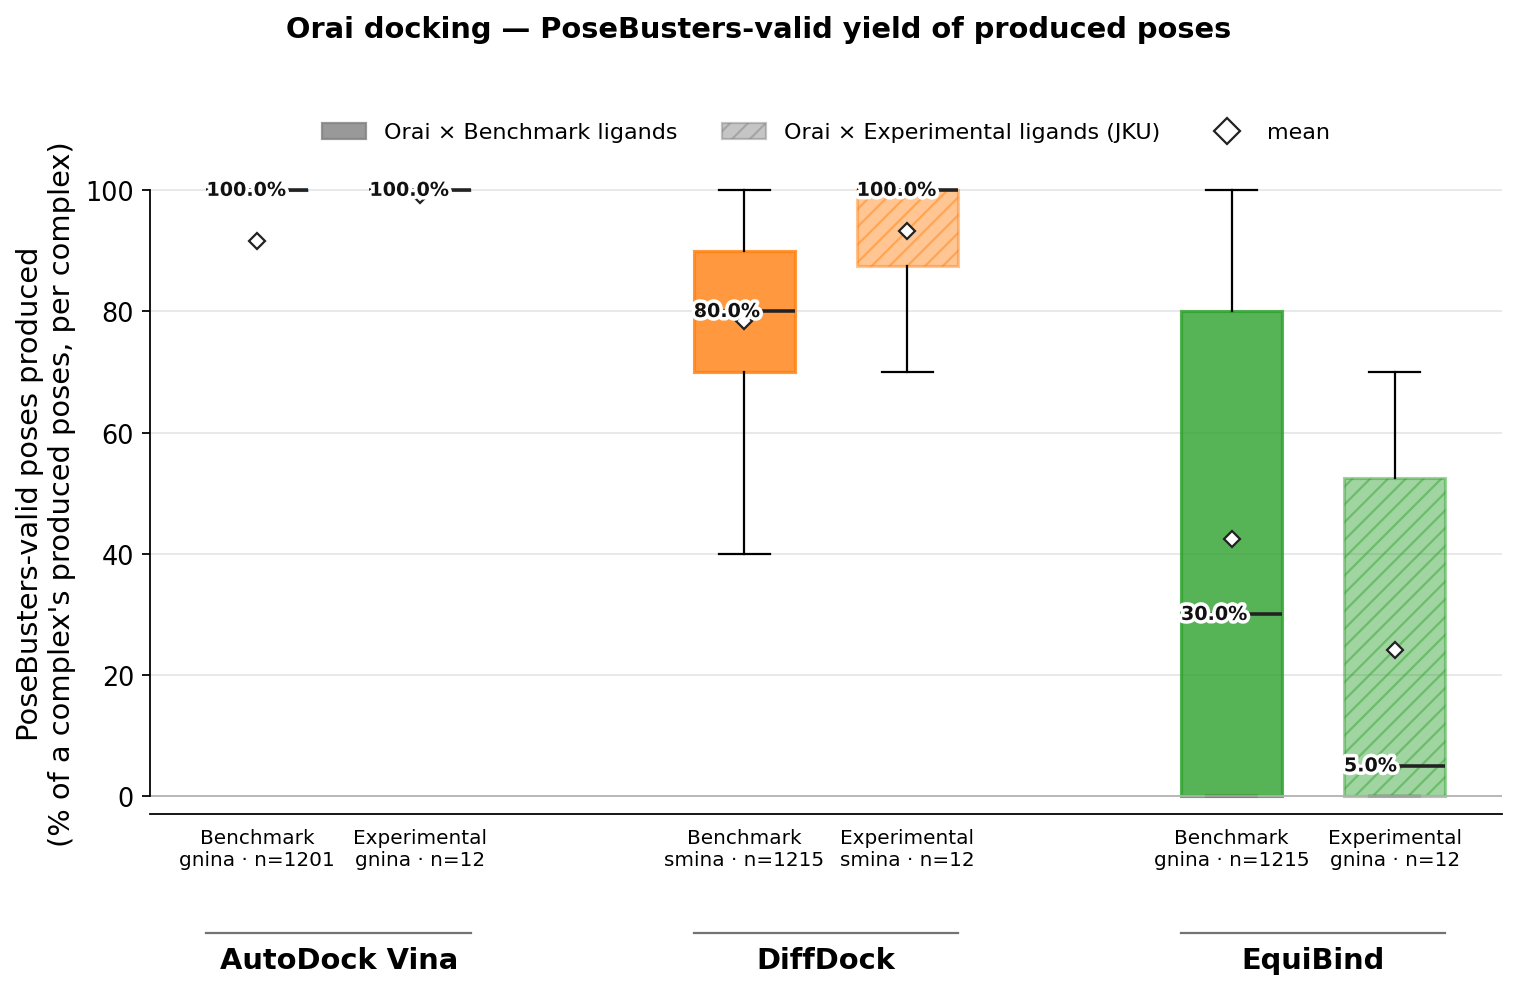
\includegraphics[width=\linewidth,height=0.78\textheight,keepaspectratio]{media/media/image13.png}
\caption{PoseBusters-valid yield of produced poses on Orai}\label{fig:results-r11}
\end{figure}

Figure~\ref{fig:results-r11} shows the smallest cross-panel change for AutoDock Vina. Median validity is 100\% in both panels, and the experimental mean is 100.0\% compared with 99.1\% in the benchmark. EquiBind changes most, from a benchmark median of 60\% and mean of 52.5\% to an experimental median of 100\% and mean of 89.2\%. DiffDock also improves, from a benchmark median of 80\% and mean of 78.5\% to an experimental median of 100\% and mean of 93.3\%. Fully valid units further distinguish the tools. Their benchmark rates are 97.0\% for AutoDock, 22.2\% for DiffDock and 22.9\% for EquiBind, rising to 100.0\%, 66.7\% and 83.3\% on the experimental ligands. EquiBind remains the most dispersed tool on the benchmark, where its lower quartile is 10\% and 19\% of units yield no valid pose.

The comparison of three experimental ligands with 308 controls has little power. Non-significance means that no difference was detected, not that none exists. Its cross-panel result therefore reflects ligand-set and pose-selection differences and remains descriptive. The physical-validity ordering is preserved in both Orai panels, consistent with but not proof of transfer from calibration.

\hypertarget{operational-placement-and-usable-yield}{%
\subsection{\texorpdfstring{Operational Placement and Usable Yield }{Operational Placement and Usable Yield }}\label{operational-placement-and-usable-yield}}

The operational placement rule defined in the Methods tests an outer-pore hypothesis. It does not replace a near-native endpoint or provide ground truth. Figure~\ref{fig:results-r12} in Appendix~\ref{orai1-panels} illustrates the rule on Fr300. The slab extends to the outer protein shell, consistent with the radially unbounded test rather than the narrower pore lumen.

Figure~\ref{fig:results-r13} reports per-unit usable yield in both panels.

\begin{figure}[!htbp]
\centering
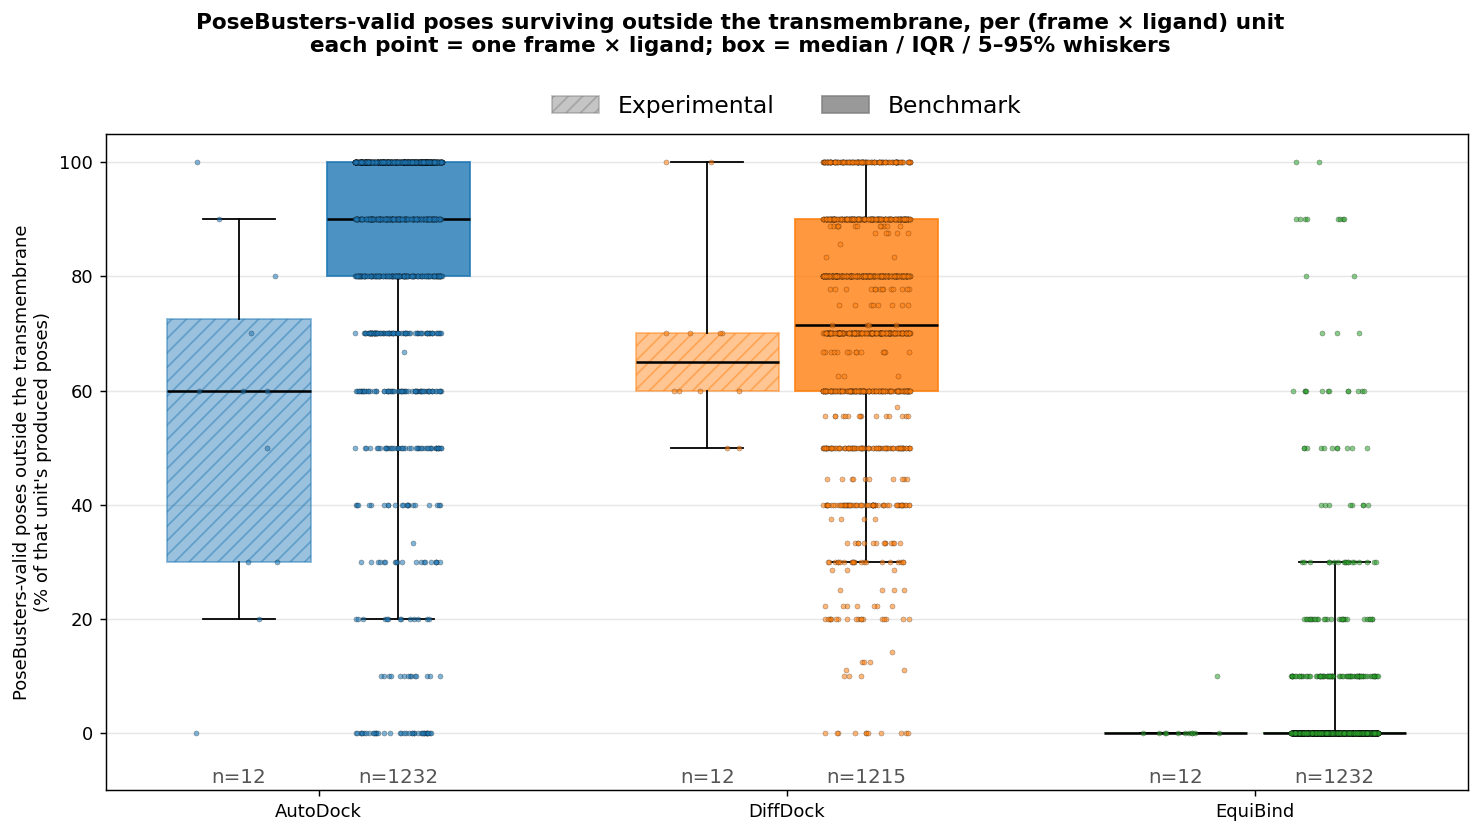
\includegraphics[width=\linewidth,height=0.78\textheight,keepaspectratio]{media/media/image43.png}
\caption{Usable pose yield per Orai frame-ligand unit}\label{fig:results-r13}
\end{figure}

AutoDock Vina leads on the benchmark but not the experimental ligands. Its medians are 90\% and 60\%, and its means 82.8\% and 54.2\%. DiffDock is lower on the benchmark (median 71.4\%) but higher experimentally (65.0\%), with means of 70.9\% and 68.3\%. EquiBind is degenerate in both panels. Its median and both quartiles are zero, with means of 3.8\% and 0.8\%.

An unpaired two-sided Mann-Whitney U test and Cliff\textquotesingle s \ensuremath{\delta}, where positive values favour the benchmark, compare frame-ligand units, removing pose nesting but not correlation among units from one ligand. AutoDock yields less experimentally than on the benchmark (U = 11749.0, \ensuremath{\delta} = +0.59, Holm p = 5.6e-4 across three tools). It is the only contrast that survives at both units and represents all three experimental ligands. The ligand-collapsed medians are 55.0\% and 92.5\% (\ensuremath{\delta} = +0.94, Holm p = 0.012). A panel-matching artefact inflates this contrast. Both panels retain ten poses, but the experimental ten are the gnina-best of thirty searched modes whereas the control ten are all that were written. Restricting the experimental panel to Vina modes one to ten moves the ligand-collapsed median from 55.0 to 70.0\% and its adjusted p from 0.012 to above 0.2, and the frame-ligand p from 5.6e-4 to 0.054 (Appendix~\ref{orai1-panels}). AutoDock still loses most between panels, but this adjusted significance does not survive matching. DiffDock trends in the same direction without significance (U = 8462.0, \ensuremath{\delta} = +0.16, p = 0.667), while EquiBind shows little change (\ensuremath{\delta} = +0.06, Holm p = 0.667).

The pooled pose-level analysis agrees but estimates rate differences rather than differences between per-unit means. These diverge for DiffDock because unit pose counts vary. AutoDock falls by 28.7 percentage points, from 82.83\% to 54.17\%, with a Fisher p below 1e-4 after correction, though the panel-matched restriction above puts that fall at 17.0 points. DiffDock changes by 2.7 points (71.07\% to 68.33\%) and EquiBind by 3.0 points (3.85\% to 0.83\%). Both are non-significant. With twelve correlated experimental units, these null results do not establish equivalence.

\begin{figure}[!htbp]
\centering
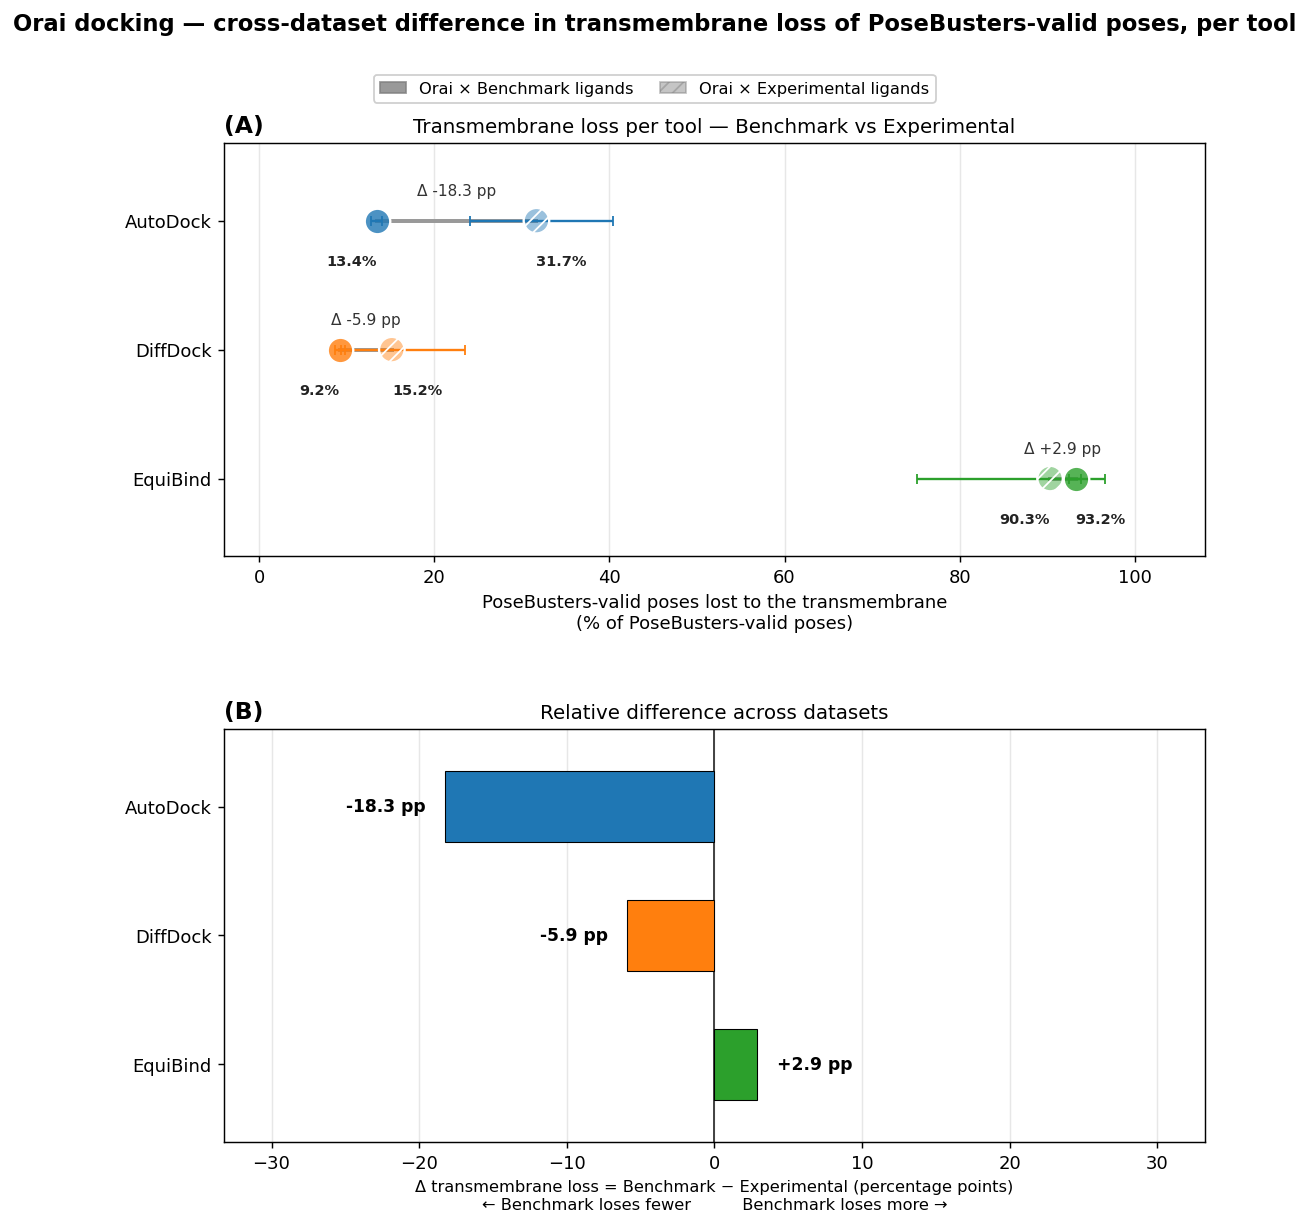
\includegraphics[width=\linewidth,height=0.78\textheight,keepaspectratio]{media/media/image15.png}
\caption{Transmembrane loss of PoseBusters-valid poses}\label{fig:results-r14}
\end{figure}

Figure~\ref{fig:results-r14} shows the proportion of PoseBusters-valid poses inside the slab under the same top-ten cap as Table~\ref{tab:results-orai-yield}. AutoDock Vina loses 16.4\% of control and 45.8\% of experimental poses, DiffDock 9.6\% and 26.8\%, and EquiBind 92.7\% and 99.1\%. These pose-level contrasts are descriptive because poses cluster within frame-ligand units. Together with Figure~\ref{fig:results-r13}, they distinguish validity from conditional placement. DiffDock loses less on both panels and therefore has higher experimental usable yield despite AutoDock Vina producing more valid poses. EquiBind almost entirely fails placement.

The per-unit usable-yield test corroborates only AutoDock Vina\textquotesingle s 29.4-point benchmark-to-experimental loss gap, at both the frame-ligand and ligand units. That gap is 17.8 points once the panels are matched on selection rule, so the corroboration is conditional on the caveat given above. The DiffDock and EquiBind gaps remain pooled descriptions. Absolute differences are preferable to ratios because the experimental denominator contains three ligands and at most twelve units, making the apparent 0.36-fold reduction in loss, which is 0.48-fold on the matched panels, unstable. Because the four frames sample one receptor, even the per-unit test is anti-conservative for generalisation to new ligands.

\hypertarget{cross-tool-clustering-1}{%
\subsection{Cross-Tool Clustering}\label{cross-tool-clustering-1}}

Clustering was performed for each MD frame, ligand and tool to assess cross-tool localisation and within-tool pose-cloud structure. Frames of one ligand are correlated snapshots of the same receptor-ligand system, so pooled medians are mildly pseudoreplicated. Collapsing each ligand across its frames gives a benchmark median of 29.3\angstrom{}, close to the pooled 28.4\angstrom{}. The experimental estimate changes from a pooled 38.1\angstrom{} to 40.3\angstrom{} after collapse and is therefore unstable, as expected from three ligands and eleven multi-tool units. Only the benchmark value is a stable central estimate.

\begin{figure}[!htbp]
\centering
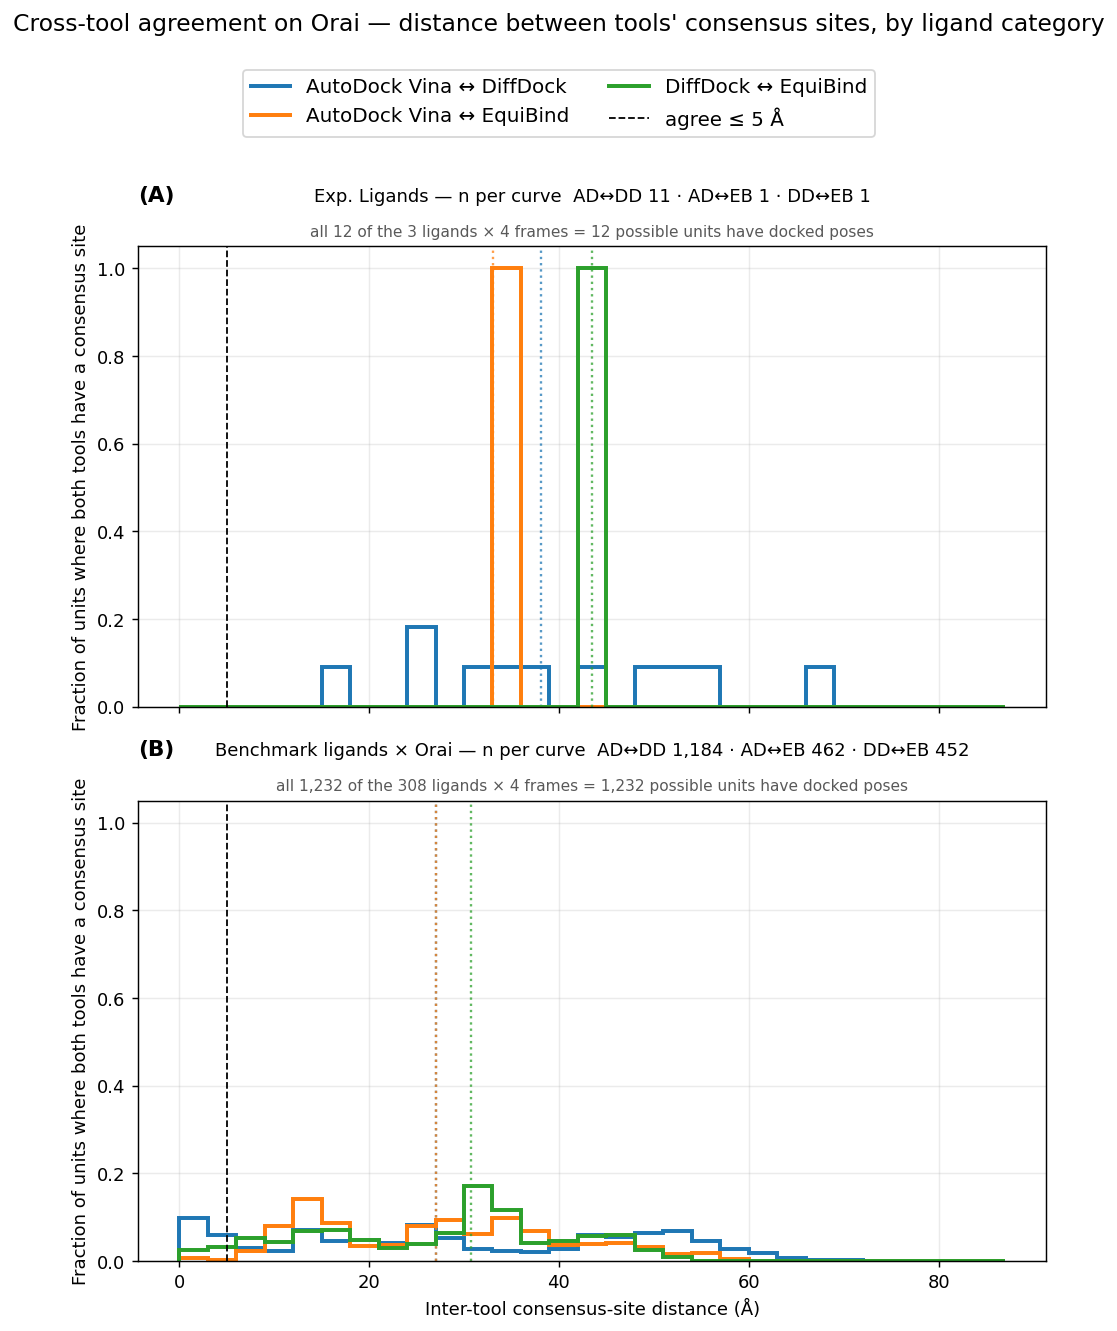
\includegraphics[width=\linewidth,height=0.78\textheight,keepaspectratio]{media/media/image16.png}
\caption{Distribution of inter-tool consensus-site distances on Orai. The dotted vertical lines mark the per-pair medians}\label{fig:results-r15}
\end{figure}

Figure~\ref{fig:results-r15} shows pairwise consensus-site distances. No experimental pair lies within the 5\angstrom{} threshold. Both benchmark EquiBind pairings are also sparse below it, whereas the tallest AutoDock--DiffDock bin lies just below 5\angstrom{}, despite most of that distribution lying above. Distances extend from a few ångströms to roughly 86\angstrom{} along the elongated pore. Pairwise medians are 27--31\angstrom{} for benchmark and 33--44\angstrom{} for experimental ligands. Continuous distances and pairwise rates are therefore more informative than the binary all-pairs flag, which requires every available pairing in a unit to lie within 5\angstrom{}. This occurs in 97 of 1,198 (8.1\%) multi-tool benchmark units and none of the eleven experimental units.

\begin{figure}[!htbp]
\centering

\includegraphics[width=\linewidth,height=0.78\textheight,keepaspectratio]{media/media/image17.png}
\caption{Cross-tool agreement on Orai}\label{fig:results-r16}
\end{figure}

Figure~\ref{fig:results-r16} resolves agreement by tool pair. For this endpoint, positive Cliff\textquotesingle s \ensuremath{\delta} means greater separation experimentally, opposite to the benchmark-higher orientation used for yield and cluster quality. The largest gap is DiffDock--EquiBind, at 43.5\angstrom{} experimentally versus 30.7\angstrom{} on the benchmark (\ensuremath{\delta} = +0.78). The contrast does not survive correction, and ligand-level collapse retains a single experimental ligand because neither Synta-66 nor GSK-7975A produced an EquiBind pose surviving the slab filter and top-ten cap. This is an exploratory estimate, not a corrected finding. The other two pairings are flat. AutoDock and DiffDock lie within 5\angstrom{} in 14\% of benchmark pairs but none of eleven usable experimental pairs. EquiBind pairings remain at or below 4\% on the benchmark and zero experimentally. Across all three pairings, 9\% of benchmark pairs and none of thirteen experimental pairs agree. Three-way agreement, which requires all three distances within 5\angstrom{}, occurs in two of 450 benchmark units with all three tools and not in the single experimental unit. AutoDock--DiffDock is therefore the only material agreement channel.

Reference-free cluster quality is reported in Figure~\ref{fig:results-r17} in Appendix~\ref{orai1-panels}, over six metrics on the raw pose cloud. DiffDock forms the tightest experimental clouds and EquiBind the loosest, often one diffuse mode. Only DiffDock\textquotesingle s Calinski-Harabasz index survives collapsing each ligand across four frames, and the appendix reads that as removal of within-ligand spread rather than new evidence.

Restricting benchmark clouds to PoseBusters-valid, outside-slab poses leaves within-cluster spread essentially unchanged for all three tools. Bootstrap stability rises significantly for all three, and DiffDock also improves on silhouette. Filtering increases reproducibility rather than tightness. Appendix~\ref{orai1-panels} gives the paired per-unit tests in Figure~\ref{fig:results-r18}, including the reduced EquiBind subset and degenerate single-cluster clouds that inflate its stability gain. Filtering does not detectably reduce the wide pore-axis scatter. Because no equivalence test was run, this bounds the observed filtering effect without establishing that the scatter is intrinsic to sampling.

AutoDock Vina forms the best-separated clouds and the tightest benchmark clouds, but precision without a reference does not establish accuracy. The broadly preserved ordering supports only cautious descriptive use of the control panel, not equivalence.

\protect\hypertarget{_Toc235735939}{}{}

\hypertarget{interaction-and-contact-analysis-1}{%
\subsection{Interaction and Contact Analysis}\label{interaction-and-contact-analysis-1}}

The analysis includes each tool\textquotesingle s top three PoseBusters-valid, outside-slab poses per frame-ligand unit. Both panels use the same four frames, making their residue axes directly comparable. PandaMap assigns residue-level contacts to fifteen interaction classes. After filtering, the experimental panel contains 32 poses from 11 AutoDock complexes and 36 from 12 DiffDock complexes, compared with 3,541 and 3,524 benchmark poses. EquiBind retains one experimental pose and 324 benchmark poses. Its results are non-interpretable and shown only for completeness. Figures display pose-level values, but significance tests first aggregate correlated poses to per-complex means. Contact-count and type-profile comparisons use unpaired Mann-Whitney U tests and Cliff\textquotesingle s \ensuremath{\delta}, with positive values favouring the benchmark.

Experimental poses have descriptively more contacts. The median rises from 27 to 30 for AutoDock Vina and from 15 to 18 for DiffDock. Neither difference survives per-complex testing, and collapsing each ligand across four frames leaves both untested, strengthening the AutoDock effect and weakening the DiffDock one. EquiBind\textquotesingle s single usable experimental pose is untestable and excluded from the correction family. No total-contact difference is detected at the available power, which does not establish equivalent contact intensity. Figure~\ref{fig:results-r19} in Appendix~\ref{orai1-panels} reports the distributions and four effect sizes.

\begin{figure}[!htbp]
\centering

\includegraphics[width=\linewidth,height=0.89\textheight,keepaspectratio]{media/media/image21.png}
\caption{Interaction-type profile on Orai}\label{fig:results-r20}
\end{figure}

Figure~\ref{fig:results-r20} reports mean interaction counts per pose. Alkyl-\ensuremath{\pi}, hydrophobic, other \ensuremath{\pi} and hydrogen-bond interactions dominate under both mature tools, but their order changes. Hydrogen bonds rank second on the benchmark and fifth experimentally. Benchmark ligands form more hydrogen bonds (Cliff\textquotesingle s \ensuremath{\delta} = +0.45 for AutoDock and +0.54 for DiffDock) and all ionic, salt-bridge and attractive-charge contacts. These charged classes are absent from both tools\textquotesingle s modulator poses. Modulators are more hydrophobic (\ensuremath{\delta} = \ensuremath{-}0.59 and \ensuremath{-}0.58) and richer in alkyl-\ensuremath{\pi} contacts (\ensuremath{-}0.42 and \ensuremath{-}0.59). They also register more halogen bonds, but that result carries no weight because the profiler is blind to chlorine and bromine and misses chlorine in part of the control library (Appendix~\ref{interaction-fingerprints}).

These patterns remain descriptive. At the frame-ligand unit, fourteen of twenty-six tool-by-type cells pass Benjamini-Hochberg correction. Two are the discounted halogen-bond cells, leaving twelve interpretable cells. None passes at the ligand unit, where the smallest adjusted values are 0.089 and 0.106. Table~\ref{tab:appendix-orai-interaction} gives the corresponding mean counts. The common direction is chemically plausible because the modulators are halogenated and lipophilic, whereas the benchmark library is more polar and hydrogen-bond driven, but it is not an established panel difference.

Both panels concentrate contacts on Asp110, Gln108, Tyr115, His113, Pro201 and Leu202. No residue differs after Holm correction of the fifteen within-tool tests. Figure~\ref{fig:results-r21} in Appendix~\ref{orai1-panels} gives the residue profiles.

\begin{figure}[!htbp]
\centering

\includegraphics[width=\linewidth,height=0.78\textheight,keepaspectratio]{media/media/image23.png}
\caption{Contact-fingerprint overlap between the two ligand sets}\label{fig:results-r22}
\end{figure}

Figure~\ref{fig:results-r22} compares contacted residues between panels. Residue-level Jaccard overlap is 0.42 for AutoDock and 0.31 for DiffDock, falling to typed-contact values of 0.40 and 0.27. Because all values use the same 10\% characteristic-contact threshold, these declines reflect changed interaction types rather than a changed basis. AutoDock shares 26 characteristic residues and DiffDock 13. EquiBind shares 5, but its overlap is uninterpretable from one experimental pose. The 10\% threshold also corresponds to roughly four experimental poses but several hundred benchmark poses. Diverse benchmark ligands distribute contacts broadly, whereas three repeatedly docked modulators concentrate them. The larger experimental-only count therefore reflects set size and homogeneity, not promiscuity. Shared residues and per-residue frequencies are more robust.

The surviving modulator poses partially agree with published pharmacology. Synta-66 maps to an extracellular TM1/TM3 region and adjoining loops near the E106 selectivity filter \cite{ref071}. Its defining extracellular loop1 and loop3 residues (His113, Tyr115, Pro201 and Leu202) lie above the filter and are characteristic of both tools\textquotesingle{} modulator poses. Leu109 is characteristic of both tools on the benchmark panel but of neither experimentally, at 9.4\% for AutoDock Vina and 5.6\% for DiffDock. Phe199 is characteristic of AutoDock Vina in both panels and of DiffDock only experimentally, where 19.4\% of poses contact it compared with 6.3\% on the benchmark. Each tool produces one modulator pose contacting Glu106, so neither consistently recovers the filter residue. These contacts support biological interpretation and hypotheses for mutagenesis or ligand-bound simulation, but evidence from different tools cannot be combined to validate one binding mode.

Net usable yield reverses the control-panel ordering. AutoDock Vina leads on controls, while DiffDock leads experimentally. Calibration point estimates show the same ordering, although not a statistically separable difference. EquiBind loses 106 of 107 valid poses to the exclusion rule and retains one of 120.

Three conclusions follow. First, physical validity alone overstates utility on a channel because a geometrically valid pose may occupy the ion-conduction pathway. Usable yield exposes EquiBind\textquotesingle s placement failures. Second, cross-tool consensus provides no reliable confidence signal. Median separation is roughly 30\angstrom{} on the benchmark and at least as large experimentally, although the experimental median is unstable after frame-robust collapse. At best 14\% of pairs agree within 5\angstrom{}. Symmetry folding is not applied to these separations. A rotation about the pore leaves the axial offset untouched and can shorten only the transverse part, so the six-fold symmetry of the channel cannot reconcile placements that differ along the pore. Appendix~\ref{orai1-panels} reports the separations without any symmetry correction. All three tools agree in two of 450 benchmark units and no experimental unit. Filtering valid, outside-slab poses does not detectably tighten the scatter, but without an equivalence test this only bounds the observed filtering effect.

Third, retained poses contain descriptive chemical signal. Both panels contact the same pocket residues, while modulators are more hydrophobic and less hydrogen-bonded, consistent with their halogenated lipophilic chemotypes. Both tools contact His113, Tyr115, Pro201 and Leu202. This does not conflict with large consensus-site distances. That metric uses each tool\textquotesingle s largest cluster, whereas residue sets pool all retained poses after six-fold symmetry folding. Arg170, Leu174 and Ala177 define an AutoDock-only sub-pocket below the Arg91 ring on the cytosolic face, associated with the Lys85 cluster. A further AutoDock cluster lies around Lys85 and neighbouring residues on the N-terminal segment below TM1. Neither cytosolic cluster supports the Synta-66 concordance. Both are reported for completeness.

Cross-panel agreement is limited. 19 of 54 testable contrasts have adjusted p below 0.05 at the frame-ligand unit and two at the ligand unit. The sensitivity analysis identifies one of the latter, DiffDock\textquotesingle s Calinski-Harabasz index, as a collapse artefact. AutoDock Vina\textquotesingle s lower experimental usable yield is the only result significant at both units and supported by all three ligands. It is the strongest cross-panel observation but remains descriptive, both because three ligands and four snapshots of one receptor cannot support general inference and because its adjusted significance does not survive matching the two panels on selection rule. For Orai1 the practical recommendation is therefore to retain AutoDock Vina and refined DiffDock as separate hypothesis generators, to prioritise poses that satisfy the validity and placement rules and agree with independent pharmacology, and to omit EquiBind in its present configuration. Sparse overlap between the two viable tools should not itself be treated as validation.

\hypertarget{pose-production-costs}{%
\section{Pose Production Costs}\label{pose-production-costs}}

Cost is normalised per qualifying pose, defined as PoseBusters-valid and within 2\angstrom{} of the crystal ligand. All docking used one workstation, whose specification and stage-specific devices are given in Appendix~\ref{docking-protocols}.

All figures use the whole-protein run of 303 complexes. The blind Vina search at exhaustiveness 128 took 4.73 wall-hours and gnina rescoring consumed 10.27 GPU-hours of device occupancy, making the rescorer roughly twice as expensive as the search it re-ranks. AutoDock therefore required 15.00 charged hours, 68.5\% for rescoring. Per-pose values divide this total.\footnote{Cost is charged as device occupancy throughout, on the single basis defined in the Methods: CPU-core-seconds divided by the 32 hardware threads of the workstation, plus GPU-seconds. Search and rescoring consume 151.42 CPU-core-hours and 10.27 GPU-hours. The CPU value is the search wall multiplied by 32 requested threads rather than measured occupancy, so dividing it by 32 returns the 4.73 wall-hours the search actually took and the charged total is that search time plus the rescorer's device occupancy. The rescoring pass was run sixteen ways concurrently and finished in 0.74 wall-hours, so its wall clock is a scheduling result rather than a property of the method. Charging it at wall clock instead would put AutoDock at 5.47 total wall-hours with 13.5\% for rescoring, and would flatter this arm against the pipelines it is compared with. The pass therefore summed roughly fourteen times its own wall clock across the sixteen workers, which changes elapsed time without changing the work done. Because neither CPU-core-seconds nor GPU-seconds are divided by that worker count, the charged basis is unaffected by it, whereas measured elapsed time is not.}

\begin{figure}[!htbp]
\centering

\includegraphics[width=\linewidth,height=0.78\textheight,keepaspectratio]{media/media/image24.png}
\caption[Charged seconds per qualifying pose]{Charged device-occupancy seconds per qualifying pose. Each box covers that pipeline's own 199, 169 and 80 qualifying complexes, while the bracketed tests use the 53 all three share}\label{fig:results-r23}
\end{figure}

\begin{longtable}[]{@{}
  >{\raggedright\arraybackslash}p{(\columnwidth - 12\tabcolsep) * \real{0.1600}}
  >{\raggedleft\arraybackslash}p{(\columnwidth - 12\tabcolsep) * \real{0.1400}}
  >{\raggedleft\arraybackslash}p{(\columnwidth - 12\tabcolsep) * \real{0.1700}}
  >{\raggedleft\arraybackslash}p{(\columnwidth - 12\tabcolsep) * \real{0.1200}}
  >{\raggedleft\arraybackslash}p{(\columnwidth - 12\tabcolsep) * \real{0.1500}}
  >{\raggedleft\arraybackslash}p{(\columnwidth - 12\tabcolsep) * \real{0.1200}}
  >{\raggedleft\arraybackslash}p{(\columnwidth - 12\tabcolsep) * \real{0.1400}}@{}}
\caption[Cost per Qualifying Pose]{Cost per Qualifying Pose. Charged medians and interquartile ranges are taken over the complexes for which that pipeline produced a qualifying pose. One basis applies to all four rows, namely CPU-core-seconds divided by the 32 hardware threads of the workstation plus GPU-seconds, so the charged column is directly comparable across pipelines. The CPU-core-second and GPU-second columns are pooled aggregates in their own currencies and are never summed}\label{tab:results-cost-per-qualifying-pose}\tabularnewline
\toprule\noalign{}
Pipeline & \shortstack[r]{Charged\\ median (s)\strut} & \shortstack[r]{Interquartile\\ range (s)\strut} & Complexes & \shortstack[r]{CPU-core-\\ seconds\strut} & \shortstack[r]{GPU-\\ seconds\strut} & \shortstack[r]{Qualifying\\ poses\strut} \\
\midrule\noalign{}
\endfirsthead
\toprule\noalign{}
Pipeline & \shortstack[r]{Charged\\ median (s)\strut} & \shortstack[r]{Interquartile\\ range (s)\strut} & Complexes & \shortstack[r]{CPU-core-\\ seconds\strut} & \shortstack[r]{GPU-\\ seconds\strut} & \shortstack[r]{Qualifying\\ poses\strut} \\
\midrule\noalign{}
\endhead
\bottomrule\noalign{}
\endlastfoot
AutoDock & 137.2 & 75.6 to 167.4 & 199 & 1,752.8 & 118.9 & 311 \\
DiffDock & 49.4 & 14.1 to 127.3 & 169 & 2.93 & 49.9 & 1,622 \\
EquiBind & 2.4 & 1.0 to 7.3 & 80 & 165.3 & 1.4 & 466 \\
\midrule\noalign{}
AutoDock, Vina search only & 21.7 & 9.9 to 45.3 & 202 & 1,805.0 & 0.0 & 302 \\
\end{longtable}

The configured AutoDock pipeline is the most expensive route to a qualifying pose under blind whole-protein search. Figure~\ref{fig:results-r23} shows the per-complex charged distributions, and Table~\ref{tab:results-cost-per-qualifying-pose} reports all three currencies. Among 53 complexes where every tool succeeds, the ordering persists (Friedman \ensuremath{\chi}\textsuperscript{2} = 85.2, p = 3.2e-19, Kendall W = 0.80), and every pair passes Holm correction. Median per-complex cost ratios are 0.14 for DiffDock versus AutoDock and 0.02 for EquiBind. gnina raises AutoDock cost to roughly three times the search alone, then that total is amortised over few qualifying poses. The median successful complex yields one, although 199 of 303 complexes now yield at least one, far more than the 169 of DiffDock.

Tightening the endpoint increases cost most for AutoDock. Median charged seconds per generated, valid, and valid-near-native pose are 5.3, 5.3 and 137.2 for AutoDock. The DiffDock values are 7.6, 9.2 and 49.4, and the EquiBind values are 0.3, 0.4 and 2.4. Contributing complexes fall from 303 to 301 to 199 for AutoDock, 303 to 300 to 169 for DiffDock, and 303 to 266 to 80 for EquiBind. Moving from valid to valid-near-native multiplies unit cost by about 25.9, compared with 5.4 for DiffDock and 6.0 for EquiBind. The multiplier is large for AutoDock because a complex that succeeds contributes only one or two qualifying poses out of thirty, not because it succeeds rarely. EquiBind\textquotesingle s 2.4 s median describes only the 80 successful complexes. It fails in the other 223.

\begin{figure}[!htbp]
\centering

\includegraphics[width=\linewidth,height=0.78\textheight,keepaspectratio]{media/media/image25.png}
\caption{Hardware resource per qualifying pose. The two currencies are pooled aggregates and are never summed}\label{fig:results-r24}
\end{figure}

Removing parallelism from the resource axis widens the separation (Figure~\ref{fig:results-r24} and Table~\ref{tab:results-cost-per-qualifying-pose}). Configured AutoDock is most expensive on every axis. Its 32 threads compress 151.42 CPU-core-hours of search into 4.73 wall-hours. The subsequent GPU rescoring pass adds device occupancy without adding CPU cost. The tools convert their compute into 311, 1,622 and 466 qualifying poses, which explains much of the gap. GPU time covers docking for DiffDock and EquiBind but only gnina rescoring for AutoDock. AutoDock nevertheless has the highest GPU cost per qualifying pose because its qualifying yield is low.

Four caveats apply. First, wall-clock time is cross-hardware and device mixes differ within and between pipelines. AutoDock spends 4.73 of its 15.00 charged hours on a multithreaded CPU and 10.27 on a GPU shared by up to sixteen concurrent workers, so elapsed time does not measure identical work. Second, resource values are order-of-magnitude estimates. AutoDock CPU-core-seconds cover only Vina and assume all 32 threads are occupied, while gnina is recorded separately as GPU occupancy. Third, part of the AutoDock rescoring pass is an implementation artefact. The rescorer was invoked once per pose, and each invocation paid the start-up of a separate process on a GPU that a single-pose evaluation leaves substantially idle. Batching would therefore reduce the cost of the learned rescorer by an amount this run does not determine. Fourth, the charged basis credits every pipeline with full use of the 32 threads, which the three arms did not realise equally. Vina already occupies all 32 within a single docking, whereas EquiBind reaches that occupancy only by running separate complexes concurrently, so its charged figure is an idealised best-configuration estimate rather than a measured elapsed time. Its 21.39 CPU-core-hours are under a seventh of AutoDock\textquotesingle s 151.42. The uniform basis therefore makes the three columns arithmetically comparable without making the underlying concurrency equally attainable, and EquiBind\textquotesingle s figure should be read as a floor. The pooled resource panel has no inferential test, but pipeline success differs strongly at the complex level (Cochran\textquotesingle s Q = 61.1, p = 5.5\ensuremath{\times}10\textsuperscript{\ensuremath{-}14}).

Under the blind whole-protein configuration used throughout this chapter, configured AutoDock is most expensive per qualifying pose in charged, CPU and GPU terms. This does not apply to the classical search alone. Without gnina, Vina requires a median 21.7 s and no GPU time per qualifying pose, still below DiffDock on the charged basis. Its CPU cost per qualifying pose is 1,805.0 s, higher than the rescored arm\textquotesingle s 1,752.8 s, because rescoring adds nine qualifying poses at no CPU cost. Vina remains by far the most processor-intensive engine on either arm, while AutoDock becomes most expensive in charged and GPU time only after learned rescoring. It is also not cheapest per generated pose on any currency (Table~\ref{tab:appendix-cost-per-pose}). Its advantage is coverage and admissibility, not economy.

The ordering depends on the denominator rather than on the currency. Median charged time per attempted docking is 157.7 s for AutoDock, 227.6 s for DiffDock and 8.1 s for EquiBind. Because each produces about thirty poses per complex, this rescales the per-complex median rather than providing an independent measure. Allocating the whole campaign to complexes that yield a qualifying pose gives 271, 479 and 38 s. On this denominator AutoDock is cheaper than DiffDock in charged and GPU terms, with 186 versus 478 GPU-seconds per success, but remains much more expensive in CPU-core-seconds. Neither denominator changes the per-qualifying-pose result.

\hypertarget{discussion}{%
\chapter{\texorpdfstring{Discussion }{Discussion }}\label{discussion}}

\hypertarget{principal-findings-and-scope-of-inference}{%
\section{Principal Findings and Scope of Inference}\label{principal-findings-and-scope-of-inference}}

This study compared AutoDock Vina, DiffDock and EquiBind by crystallographic re-docking of 303 calibration complexes and reference-free docking of three Orai1 modulators into four molecular-dynamics snapshots. The calibration benchmark provides stronger evidence because each prediction has an experimental reference. Its endpoints favour AutoDock without settling the comparison. Under the blind whole-protein search, AutoDock had the highest physical validity and led DiffDock on near-native recovery and native-pocket reach at every depth. The near-native lead is inconclusive at rank-1 and separable from top-5 onwards, and reach never separated them. The rank-1 interval spans a 4.2-point DiffDock lead to a 9.4-point AutoDock lead. Refined EquiBind had low raw validity, in-place accuracy and pocket localisation. Orai1 preserved the validity ordering but reversed the usable-yield ordering. Without a ligand-bound structure, neither result identifies the correct binding mode.

These findings rank the configured pipelines, not artificial intelligence and physics as method classes. Newer diffusion, co-folding and hybrid systems report gains from specified pockets, receptor flexibility and structural relaxation \cite{ref012}, \cite{ref031}, \cite{ref064}, \cite{ref069}. Similarity-controlled and perturbation analyses also show that aggregate accuracy can conceal reliance on training-set analogues and weak extrapolation to new pockets \cite{ref035}, \cite{ref063}, \cite{ref065}, \cite{ref069}. This thesis therefore contributes a separation of sampling, ranking, validity and localisation failures rather than a permanent method ranking.

Physics-based is itself an operational label here. Vina combines explicit search with an empirical score. It is not a molecular-mechanics or free-energy simulation. Its result supports the evaluated classical search-and-score workflow, not a complete physical model of binding.

\hypertarget{physical-validity-and-post-docking-optimisation}{%
\section{Physical Validity and Post-Docking Optimisation}\label{physical-validity-and-post-docking-optimisation}}

The largest initial separation preceded RMSD assessment. Under the blind whole-protein configuration used here, pooled validity differed by more than seventy percentage points between AutoDock Vina and the raw learned outputs. Local optimisation then made many learned poses admissible. This margin is partly constitutive because the discriminating intermolecular checks inspect coordinates already minimised by Vina, as Appendix~\ref{validity-objective-coupling} explains. Its effect on the headline endpoint is small, however. Requiring validity removes at most four of 303 complexes at any depth. RMSD alone is therefore insufficient, since a geometrically close ligand can still have unrealistic bonds, steric overlap or intermolecular contacts \cite{ref035}. Combined accuracy and validity are more discriminating \cite{ref013}, \cite{ref032}.

Local optimisation mainly repaired geometry, not blind placement. DiffDock validity rose sharply while its fixed-rank near-native rate barely changed. EquiBind showed a modest near-native increase. Table~\ref{tab:appendix-refinement-bands} reports these changes by rank band.

Refiner selection remains an empirical pipeline choice, and the two families behave differently. For DiffDock the refiners are interchangeable. smina is carried forward on the selection criterion by 133 complexes to 132, but that one-complex margin survives only in the three-way conjunction of validity, near-nativeness and form. Dropping either the validity or the form term leaves the two arms exactly level, and gnina is level or ahead on every component taken alone. Exact McNemar separates them at no depth. For unguided EquiBind the choice is not immaterial. gnina recovers 83 near-native complexes at top-15 against 61 for smina, and that difference survives Holm correction. Only on the selection endpoint, where the margin is nine complexes, are the two EquiBind arms not separable. The study measured neither optimisation trajectories nor refiner performance on an independent set, so proposed mechanisms such as gentle preservation or aggressive repair remain interpretations.

PoseBusters validity is not binding stability. Passing Table~\ref{tab:appendix-posebusters-checks} excludes important chemical, conformational and steric failures but establishes neither favourable binding free energy, correct protonation or tautomer states, water or ion mediation, nor persistence in a membrane. Validity is an admissibility filter. Placement, interaction recovery and prospective experiments test accuracy separately.

\hypertarget{sampling-ranking-and-interaction-recovery}{%
\section{Sampling, Ranking and Interaction Recovery}\label{sampling-ranking-and-interaction-recovery}}

Ranking depth separates generation from selection. Moving from rank-1 to the best of fifteen substantially increased recovery for DiffDock and AutoDock but added only about eight percentage points for EquiBind (Results, Near-Nativeness and Form). Useful DiffDock and AutoDock poses were therefore often under-ranked. Selection was not the main loss. About six in ten rank-1 failures of the two tools contained no qualifying pose at any depth. The corresponding share for EquiBind was about nine in ten. Re-ranking cannot recover an absent binding mode.

The form decomposition supports this result. AutoDock and DiffDock were indistinguishable on internal form at the prespecified 1\angstrom{} Kabsch threshold, while AutoDock led on near-nativeness from top-5 onwards. DiffDock often generated a credible conformation without ranking it first. EquiBind was weaker on both axes. A ligand can retain its shape while presenting its pharmacophore to the wrong residues, so form and placement must remain distinct.

Pocket recovery was easier than exact pose recovery under the whole-protein search. AutoDock and DiffDock intervals overlapped throughout. AutoDock had the higher point estimate at top-15, but the paired reach test in the calibration Cross-Tool Clustering section did not separate them. Pooling all tools placed the crystal pocket somewhere in the pose cloud for 95\% of complexes, but the best inexpensive cluster rule ranked it first in only 57\%. This is a site-selection gap, not 95\% exact-pose accuracy. Cluster membership is coarser than a valid pose within 2\angstrom{}.

Interaction fingerprints show the same dependence on endpoint and depth. DiffDock had the highest mean crystal overlap for the union of top-five contacts, but the leading tools were not separable at rank-1. This is inconclusive rather than equivalent. The one equivalence statement in this work covers the valid-near-native recovery contrast, and its margin was read off the data after the fact rather than prespecified. AutoDock contact recovery declined through its top five while DiffDock remained flat, yet DiffDock confidence was not detectably associated with interaction recovery. AutoDock therefore ranked a weaker pool more effectively, and EquiBind missed more native contacts than it recovered at every rank. External scores require validation for their intended task \cite{ref067}.

\hypertarget{generalisation-in-the-context-of-current-literature}{%
\section{Generalisation in the Context of Current Literature}\label{generalisation-in-the-context-of-current-literature}}

The benchmark\textquotesingle s post-2021 construction reduces temporal overlap with early training data but cannot exclude homologous receptors, familiar pockets or related ligands. PoseBusters performance declined at low receptor sequence identity \cite{ref035}, and Li et al. identified pocket novelty as a central generalisation constraint \cite{ref013}. On the PDBbind time split, the TEMPL baseline rose from 22.1\% overall to 67.3\% when related protein and ligand templates were available, then collapsed outside that region \cite{ref065}. Time alone therefore does not establish novelty.

PoseBench likewise found that modern co-folding systems outperformed several conventional and learned baselines overall but remained challenged by new binding poses and the joint demands of structural accuracy and chemical specificity \cite{ref069}. PoseX reported gains from recent AI and co-folding systems after relaxation and from pocket information and physics-inspired post-processing \cite{ref012}. Performance therefore depends on model generation, benchmark novelty, receptor information, flexibility and relaxation. EquiBind\textquotesingle s result is consistent with early one-shot models trailing newer systems. The DiffDock result identifies limits of this version\textquotesingle s blind placement, validity and confidence ranking, not a ceiling on generative docking.

\hypertarget{interpretation-of-the-reference-free-orai1-study}{%
\section{Interpretation of the Reference-Free Orai1 Study}\label{interpretation-of-the-reference-free-orai1-study}}

Orai1 is more realistic but less identifiable than crystallographic re-docking. AutoDock Vina produced valid poses for all three modulators but retained a smaller share after the combined on-receptor and transmembrane-placement screen. Refined DiffDock had lower validity but more usable poses. That ordering depends on the ranking each pipeline applies before the cap, since the gnina re-ranking that improves AutoDock rank-1 recovery on the crystal benchmark selects against the placement rule here, and reverting AutoDock to its Vina order restores it to the higher yield. EquiBind retained one of 120. Without an experimental ligand pose, these rates measure admissibility rather than near-nativeness.

The R91--E106 exclusion slab encodes an outer-pore hypothesis. GSK-7975A sensitivity has been linked to filter geometry through a proposed allosteric effect rather than direct pore block \cite{ref070}, while Synta-66 has been mapped to an extracellular TM1/TM3 and loop region \cite{ref071}. Excluding the conduction pathway is therefore defensible but not ground truth. The result establishes only that EquiBind produced almost no valid, on-receptor poses outside this study\textquotesingle s slab.

Cross-tool disagreement compounds this uncertainty. AutoDock Vina and DiffDock agreed within 5\angstrom{} in none of eleven evaluable experimental pairs, compared with 14\% of control pairs, and no experimental unit had three-way consensus. The experimental distance median was unstable under frame-robust collapse, so equal scatter between panels cannot be inferred. AutoDock formed better-separated clouds and DiffDock tighter ones, but compactness measures precision, not accuracy. Recovery of literature-associated filter and TM1/TM3 residues therefore generates hypotheses. Neither partial contacts nor their combination validates a complete pose.

At the ligand unit, only AutoDock Vina\textquotesingle s lower usable yield on the modulators survived the experimental-versus-control analysis, and that survival is itself conditional on the two panels being capped by different selection rules (Appendix~\ref{orai1-panels}). Other placement, clustering and interaction contrasts either lost corrected significance or rested on one or two ligands. Three chemotypes, four correlated frames and almost no EquiBind output give little power to establish either differences or equivalence. Physical-validity ordering transferred across panels, whereas usable-yield ordering reversed, so the control panel supports only cautious reference-free comparison. A stronger study would add independent trajectories, systematic frame selection, explicit membrane and ion conditions, ligand-bound simulations and experimental mutagenesis or competition assays. The experimental work lies outside this thesis and continues at Johannes Kepler University Linz (JKU).

\hypertarget{computational-efficiency-and-practical-tool-selection}{%
\section{Computational Efficiency and Practical Tool Selection}\label{computational-efficiency-and-practical-tool-selection}}

Within the whole-protein configuration, EquiBind had the shortest median charged cost per qualifying pose, followed by DiffDock and AutoDock. All three are charged on one basis, device occupancy on a 32-thread processor and a single GPU, so the ordering is a comparison of like with like. What differs is how attainable each pipeline's concurrency is, since EquiBind reaches full thread occupancy only across separate complexes, and how many complexes each ordering rests on, EquiBind succeeding on 80 of 303 against 169 for DiffDock. The ordering is therefore firmer than its magnitude. Within this protocol, configured AutoDock was the most expensive route on the charged and hardware axes. Its return was coverage and validity rather than speed.

Hybrid evidence supports this interpretation. DiffDock-Glide improves sampling through pocket-conditioned diffusion and physics-based minimisation \cite{ref064}, PoseX reports that relaxation removes many AI steric failures \cite{ref012}, gnina 1.3 improves ranking within a classical sampler \cite{ref067}, and CACHE produced experimental hits with an open hybrid workflow without establishing universal superiority \cite{ref068}. Learned generation is most useful when paired with physical validation and task-specific ranking.

\hypertarget{implications-for-docking-workflows}{%
\section{Implications for Docking Workflows}\label{implications-for-docking-workflows}}

The results support a staged workflow that generates several hypotheses, optimises local geometry, rejects invalid or biologically inadmissible structures, ranks the remainder with an endpoint-specific selector and retains uncertainty when tools disagree. Refined DiffDock and AutoDock Vina are complementary. AutoDock has higher accuracy and pocket-localisation point estimates, while DiffDock costs less per qualifying pose. Their rank-1 near-nativeness gap is unresolved. EquiBind provides too little coverage for routine use in this configuration. Its Orai1 control panel yielded only 3.8\% usable poses, compared with 82.8\% for AutoDock and 71.1\% for DiffDock.

Future comparisons should match information and compute across current flexible diffusion and packing methods \cite{ref031}, multi-pocket conditioning \cite{ref066}, hybrid refinement \cite{ref064}, co-folding systems \cite{ref012}, \cite{ref069} and template controls \cite{ref065}, using protein-, pocket- and ligand-novel splits. EquiBind was worse with an fpocket- or P2Rank-predicted pocket than without one (Appendix~\ref{equibind-pocket-guided}), which shows that pocket detection helps only if the docking model uses it effectively. Blind community evaluation can combine flexibility-aware, hybrid and leakage-controlled testing \cite{ref047} while keeping benchmark accuracy distinct from reference-free biological hypotheses.

\hypertarget{conclusions}{%
\chapter{\texorpdfstring{Conclusions }{Conclusions }}\label{conclusions}}

\hypertarget{rq1-quality-and-stability}{%
\section{RQ1: Validity, Near-Nativeness and Ranking Depth}\label{rq1-quality-and-stability}}

All pipelines searched the whole receptor, and the headline metric required PoseBusters validity and an RMSD within 2\angstrom{}. Rank-1 recovery was 36.6\% for AutoDock, 34.0\% for DiffDock and 18.2\% for EquiBind. Retrospective top-15 recovery was 65.3\%, 55.1\% and 26.4\%. The AutoDock--DiffDock rank-1 difference was +2.6 percentage points (95\% interval \ensuremath{-}4.2 to +9.4) and was not statistically resolved, although AutoDock led from top-5 onwards, by +13.2 points there (p\_holm = 7.6e-4) and +10.2 at top-15. That ordering is conditional on search effort. AutoDock ran at exhaustiveness 128, the top rung of a five-value ladder, and no measurement here speaks to what a harder search would return (Appendix~\ref{exhaustiveness-selection}). A post-hoc 90\% compatibility interval places the rank-1 difference within about eight points. It is descriptive, not a prespecified equivalence test. Both leading tools remained decisively ahead of EquiBind.

Physical validity separated the tools in the same order, at 98.9\%, 84.5\% and 62.0\%, although part of this separation is constitutive (Appendix~\ref{validity-objective-coupling}). Rank-1 native-interaction recovery likewise did not separate the leading tools. DiffDock led only for the top-five contact union. On Orai1, median usable yield under the study\textquotesingle s placement rule was 65\% for DiffDock, 60\% for AutoDock and 0\% for EquiBind. This untested reversal rests on twelve correlated units from three ligands and is descriptive. It is also conditional on the ranking cap each pipeline carries. AutoDock is capped on its gnina re-ranking, and restricting it instead to Vina modes one to ten puts it at 75\% and removes the reversal, whereas the DiffDock cap is close to neutral on this endpoint. The five-point deficit is therefore a property of the secondary ranker rather than of the search. Only one of 120 EquiBind poses passed both screens. The separate control panel put AutoDock first.

These endpoints measure static geometry, physical validity and pose placement. None of them tests thermodynamic or time-dependent stability.

\hypertarget{rq2-effect-of-post-docking-optimisation}{%
\section{RQ2: Effect of Post-Docking Optimisation}\label{rq2-effect-of-post-docking-optimisation}}

Local optimisation mainly repaired geometry. DiffDock validity rose from 24.4\% raw to 84.5\% with smina and 87.1\% with gnina. EquiBind rose from 2.9\% to 51.3\% and 62.0\%. Fixed-rank near-native rates changed by only 0.1--0.7 percentage points for DiffDock, 4.1--4.6 for EquiBind with gnina and 3.5--4.4 with smina. The larger top-\emph{k} gains in Table~\ref{tab:appendix-refinement-mcnemar} accumulate them across ranks, and gnina also re-ranks EquiBind poses. AutoDock gained by re-ranking, from 31.0\% to 36.6\% at rank-1. That single step does not clear Holm correction on its own, and the gain reaches significance only from top-5 onwards. Optimisation therefore made many learned poses admissible but could not supply a binding mode or fix gross placement.

\hypertarget{rq3-computational-efficiency}{%
\section{RQ3: Computational Cost and Accounting Basis}\label{rq3-computational-efficiency}}

Across 303 whole-protein searches, median charged cost per qualifying pose was 2.4 s for EquiBind, 49.4 s for DiffDock and 137.2 s for AutoDock. DiffDock succeeded on 169 complexes, AutoDock on 199 and EquiBind on 80. All three are charged on one basis, CPU-core-seconds divided by the 32 hardware threads of the workstation plus GPU-seconds, so the figures are comparable in basis as well as in scope. Every tool is charged for the configuration carried forward and for nothing else. AutoDock Vina and DiffDock each produced a single configuration, and for them the charged cost and the whole run are the same number. EquiBind produced nine configurations in one pass, of which only the unguided gnina configuration is reported. The remaining twentyfold EquiBind advantage over DiffDock is therefore a property of the work performed rather than of the accounting, though it is conditional on EquiBind succeeding on a quarter of the set and on a thread occupancy it reaches only across separate complexes.

Configured AutoDock was most expensive per qualifying pose in charged, CPU-core and GPU seconds. This does not apply to Vina alone. Removing gnina puts its charged and GPU cost below DiffDock, although Vina retains the highest CPU-core cost. The 4.73-hour blind search and 10.27-hour gnina pass total 15.00 charged hours, 68.5\% of which belongs to rescoring. Per-pose process start-up leaves the GPU underused, so batching should reduce this cost by an unmeasured amount. These results describe the implementations and hardware, not method classes.

\hypertarget{rq4-opportunities-and-limitations}{%
\section{RQ4: Opportunities and Limitations}\label{rq4-opportunities-and-limitations}}

The tools fail differently, which favours a staged workflow of generating candidates, optimising geometry, screening validity and placement, then ranking with an endpoint-specific selector. The evidence remains limited to single configured settings without multi-seed sweeps, a post-2021 benchmark that cannot exclude similarity leakage, and three Orai1 chemotypes across four correlated frames without a cognate structure.

AutoDock had the highest PoseBusters pass rate and in-place point estimates, but near-nativeness separated it from DiffDock only from top-5 onwards. Generation and localisation dominated failure. About six in ten AutoDock and DiffDock rank-1 failures, and nine in ten EquiBind failures, contained no qualifying pose. Selection still recovered 87 and 64 additional complexes at top-15 for the leading tools, compared with 25 for EquiBind. The result is a workflow, not a universal winner.

\hypertarget{limitations-and-future-outlook}{%
\chapter{Limitations and Future Outlook}\label{limitations-and-future-outlook}}

No method dominates under the pocket-free conditions tested here. AutoDock Vina remains limited by a rigid receptor and empirical score, so the staged hybrid workflow requires independent validation of its final hypotheses.

DiffDock stochasticity limits reproducibility. The 303-complex calibration run is one unseeded draw made before the local seed patch. Rerunning it may change the pose sample. The Orai1 experimental panel uses seed 42 and is repeatable under the recorded environment, although bitwise determinism was not tested. The unseeded Orai1 control panel supplies most reported Orai DiffDock values (Table~\ref{tab:appendix-orai-protocols}). No arm was assessed across multiple seeds.

Variant selection and evaluation use the same 303 complexes, with no held-out split. On the variant-selection endpoint at the top-15 depth at which the choice was made, the winning margins were eight complexes for AutoDock Vina, one for DiffDock and nine for EquiBind. Only the AutoDock margin is separable, and it is the one drawn from the largest field, the eight configurations of Table~\ref{tab:appendix-exhaustiveness-ladder} against three refiner arms for each learned pipeline. The largest of those margins is 3.0 percentage points of the 303, which bounds the optimism the selection can have introduced in any one family. A winner\textquotesingle s-curse correction computed per family over three arms puts it between 0.4 and 0.8 percentage points, and Appendix~\ref{exhaustiveness-selection} gives the larger correction that the eight-arm AutoDock field carries. EquiBind also confounds geometry with ranking because gnina performs both, whereas DiffDock refinement preserves rank. All three refined arms were run in the same energy-minimisation mode (\texttt{-{}-minimize}), so the calibration-benchmark validity figures are a like-for-like comparison (Appendix~\ref{docking-protocols}).

Further limits concern denominators and endpoints. Two corrected DiffDock defects are documented in Appendix~\ref{orai1-panels}. The Orai control cap was ten rather than thirty poses and was not reached in 178 of 1,215 units. Post-2021 release does not exclude leakage, and blind whole-protein AutoDock results are not comparable with published site-centred cognate re-docking. The two arms also differ on the receptor axis. Every calibration complex is re-docked into its own cognate crystal receptor, whereas the Orai1 arm docks into non-cognate molecular-dynamics snapshots of a homology model, and cognate self-docking is the easier of the two regimes, so the calibration figures bound the Orai1 expectation from above rather than predicting it. Receptor preparation also removed waters, ions, metals and cofactors for the AutoDock and DiffDock arms. A metal ion or metal-containing cofactor lies within 5\angstrom{} of the crystal ligand in 78 of the 303 calibration complexes, so recovery across that quarter of the set is measured without a coordinating partner the crystal pose depends on. The AutoDock-over-DiffDock top-15 contrast is +6.7 percentage points on the 225 metal-free complexes against +20.5 on the 78 metal-adjacent ones, so the pooled contrast averages a narrow gap with a much wider one (Appendix~\ref{autodock-vina-2}). Poses within a complex and four frames from one receptor are correlated, making the complex or trajectory the inferential unit. Best-of-top-\emph{k} and crystal-nearest clusters are oracle ceilings rather than prospective rank-1 accuracy.

PoseBusters tests gross geometry, not binding stability, and no ligand-bound dynamics were run. No endpoint reported here resolves binding free energy. Recovery, physical validity and RMSD are geometric criteria, and no score used for ranking was compared against measured affinities. Its internal-energy check depends on pose-file hydrogens, preventing direct comparison of raw and optimiser-written arms on that check. The interaction profiler misses chlorine and bromine in its halogen test and records each charged contact in three classes. Appendix~\ref{interaction-fingerprints} therefore treats those classes as one measurement. The Orai1 slab is a uniform operational hypothesis despite ligand-specific pharmacology and may exclude valid GSK-7975A or Synta-66 poses \cite{ref070}, \cite{ref071}. Cost per qualifying pose is conditional on success and therefore favours EquiBind.

AutoDock Vina requires a search box, whereas DiffDock and EquiBind localise the ligand. Equalising information therefore withheld site information from Vina. This whole-protein box is stricter than blind benchmarks that supply predicted pockets, such as PoseBench\textquotesingle s P2Rank--Vina arm \cite{ref069}, \cite{ref061}, but matches pocket-free DiffDock baselines \cite{ref024}, \cite{ref091}. The validity advantage persists under this design, although search, scoring and local optimisation remain inseparable.

A predicted-pocket Vina arm would provide an intermediate comparison. Under-sampling and blind search were separated only along the sampling axis, since no predicted-pocket Vina arm was run. Appendix~\ref{search-effort-and-box-volume} gives the box distribution and the convergence evidence, and Appendix~\ref{exhaustiveness-selection} what raising the search effort recovered.

The Orai1 poses remain computational hypotheses. Validation requires site-directed mutagenesis, competition or displacement assays and ideally a ligand-bound structure. This work continues at JKU. The reference-free arm contributes a documented, physically screened workflow for testable hypotheses, not a validated complex.


% Transparent disclosure of the assistance used for this revision and conversion.
\aitoolentry{OpenAI Codex}{Consistency review}{Prompt: ``Please conduct a very detailed review of the
thesis. Compare the numbers reported in the tables and figures and make sure
they are in line with the text.''}

\aitoolentry{Claude Code}{Code review and code documentation of the analysis
and docking scripts, verification of the reported numbers against the underlying
data, checking and correction of citations, and application of the resulting
corrections to the manuscript text}{Representative prompts: ``Review the code for
errors and bugs''; ``Please add a function description and comments.''; ``Please
perform an adversarial review of the thesis. Do all the numbers in the graphs,
tables and prose align? Are the citations valid?''; ``Can you please correct the
citations?''}

\clearpage
\printbibliography
\clearpage
\listoffigures
\clearpage
\listoftables
\clearpage
% List of abbreviations. The class already loads the acronym package (twbook.cls:114)
% and defines \listacroname (twbook.cls:175-180), which resolves to "List of
% Abbreviations" in the english build. The phantomsection/addcontentsline/chapter*
% sequence mirrors the class's own \listaitools front-matter pattern (twbook.cls:294-296).
\phantomsection
\addcontentsline{toc}{chapter}{\listacroname}
\chapter*{\listacroname}

\begin{acronym}[ETKDGv3]
\acro{APB}[2-APB]{2-aminoethoxydiphenyl borate}
\acro{AI}{artificial intelligence}
\acro{BEDROC}{Boltzmann-enhanced discrimination of the receiver operating characteristic}
\acro{BFGS}{Broyden-Fletcher-Goldfarb-Shanno}
\acro{BH}{Benjamini-Hochberg}
\acro{CC1}{coiled-coil 1 domain of STIM1}
\acro{CI}{confidence interval}
\acro{cLogP}{calculated octanol--water partition coefficient}
\acro{CNN}{convolutional neural network}
\acro{CPU}{central processing unit}
\acro{CRAC}{calcium release-activated calcium}
\acro{CUDA}{Compute Unified Device Architecture}
\acro{Da}{dalton}
\acro{EF}{enrichment factor}
\acro{ETKDGv3}{Experimental-Torsion Knowledge Distance Geometry, version 3}
\acro{GPU}{graphics processing unit}
\acro{HBA}{hydrogen-bond acceptor}
\acro{HBD}{hydrogen-bond donor}
\acro{IC50}[\ensuremath{\mathrm{IC}_{50}}]{half-maximal inhibitory concentration}
\acro{InChI}{International Chemical Identifier}
\acro{IQR}{interquartile range}
\acro{JKU}{Johannes Kepler University Linz}
\acro{MD}{molecular dynamics}
\acro{MMFF}{Merck Molecular Force Field}
\acro{MW}{molecular weight}
\acro{PB}{PoseBusters, as in PB-valid}
\acro{PC}{principal component, numbered PC1 to PC4}
\acro{PCA}{principal-component analysis}
\acro{PDB}{Protein Data Bank}
\acro{PDBQT}{Protein Data Bank format with Partial Charge (Q) and Atom Type (T)}
\acro{PLIP}{Protein-Ligand Interaction Profiler}
\acro{QED}{quantitative estimate of drug-likeness}
\acro{RBL}{rat basophilic leukaemia}
\acro{RMSD}{root-mean-square deviation}
\acro{RO5}[Ro5]{Lipinski's rule of five}
\acro{ROCAUC}[ROC-AUC]{area under the receiver operating characteristic curve}
\acro{RQ}{research question, numbered RQ1 to RQ4}
\acro{SDF}{structure-data file}
\acro{SE3}[SE(3)]{special Euclidean group in three dimensions}
\acro{SOAR}{STIM1 Orai-activating region}
\acro{STIM1}{stromal interaction molecule 1}
\acro{TM1}{transmembrane helix 1 of Orai1, with TM3 the third such helix}
\acro{TPSA}{topological polar surface area}
\acro{TRPV6}{transient receptor potential vanilloid 6}
\acro{UFF}{Universal Force Field}
\acro{VS}{virtual screening}
\end{acronym}
\clearpage

\setcounter{tablebeforeaitools}{\value{table}}
\listaitools
\setcounter{table}{\value{tablebeforeaitools}}

\clearpage
% REVIEW NOTE: The Word document's mixed manual figure/table numbering is resolved here with automatic global numbering and cross-references.
\appendix

\hypertarget{source-code-and-data-availability}{%
\chapter{Source Code and Data Availability}\label{source-code-and-data-availability}}

The source code underlying this thesis is held in the project GitHub repository, which is available from the author on request:

\begin{center}
\url{https://github.com/dthemann/master_dev}
\end{center}

\noindent The repository contains the docking drivers for the three tools (AutoDock Vina, DiffDock and EquiBind), the post-hoc optimisation (smina / gnina) and PoseBusters validity pipeline. It also carries the pose-comparison, transmembrane-exclusion, clustering and PandaMap interaction-fingerprint analyses for both the calibration benchmark and the Orai1 application. The docking and analysis outputs themselves run to several hundred thousand files and are not distributed through the repository. The author holds them and provides them on request. A regeneration guide at Scripts/Analysis/REGENERATE.md maps the figures and tables reported in this document to the output file each was taken from and to the exact command that rebuilds that output. It also states which conda environment each command needs and in which order the dependent steps must run. The guide marks explicitly the items it could not reconstruct, namely the two hand-composed molecular renders of the Orai1 receptor, one reference-free cluster-quality figure that matches its generating output in content but not byte for byte, and the tables whose provenance it did not audit.

\hypertarget{tools-and-functions}{%
\chapter{Tools and Functions}\label{tools-and-functions}}

\hypertarget{autodock-vina-1}{%
\section{AutoDock Vina}\label{autodock-vina-1}}

AutoDock Vina was designed for higher speed and pose-prediction accuracy than earlier AutoDock versions \cite{ref022}. This section gives the procedure and the scoring equations behind the summary in the Literature Review.

\hypertarget{vina-docking-procedure}{%
\subsection{Docking Procedure}\label{vina-docking-procedure}}

Docking proceeds in five steps, set out as a flow chart in Figure~\ref{fig:literature-docking-workflow}. Receptor and ligand are first prepared by removing crystallographic water, adding hydrogen atoms, assigning atom types and Gasteiger partial charges and converting to PDBQT format. The ligand\textquotesingle s rotatable bonds are declared so the search can explore conformational flexibility. A three-dimensional box then restricts where the ligand may be placed. The box may be a known pocket for computational efficiency or, as throughout this work, the whole receptor.

Vina next generates random ligand poses inside that box, each carrying translational, rotational and torsional degrees of freedom. It refines them by an iterated local search in which random perturbation is followed by local optimisation. This is computationally feasible because the scoring function is smooth and is evaluated on precomputed interaction grids, which permits fast energy evaluation and gradient-based local improvement by a BFGS-like quasi-Newton optimiser. The surviving poses are clustered by RMSD so redundant solutions are not overrepresented. The cluster representatives are ranked by predicted binding free energy, and the lowest-energy poses are returned as the most likely docking solutions.

This explicit search-and-score design is reproducible and interpretable in terms of chemical interactions and search heuristics, which is why current comparative evaluations still carry Vina as their physics-based baseline \cite{ref012}, \cite{ref013}. Later work preserved the paradigm rather than replacing it \cite{ref023}. Both smina and subsequent Vina releases extended atom typing, exposed the scoring parameters, improved local-minimisation behaviour and eased rescoring and custom scoring-function development.

\begin{figure}[!htbp]
\centering
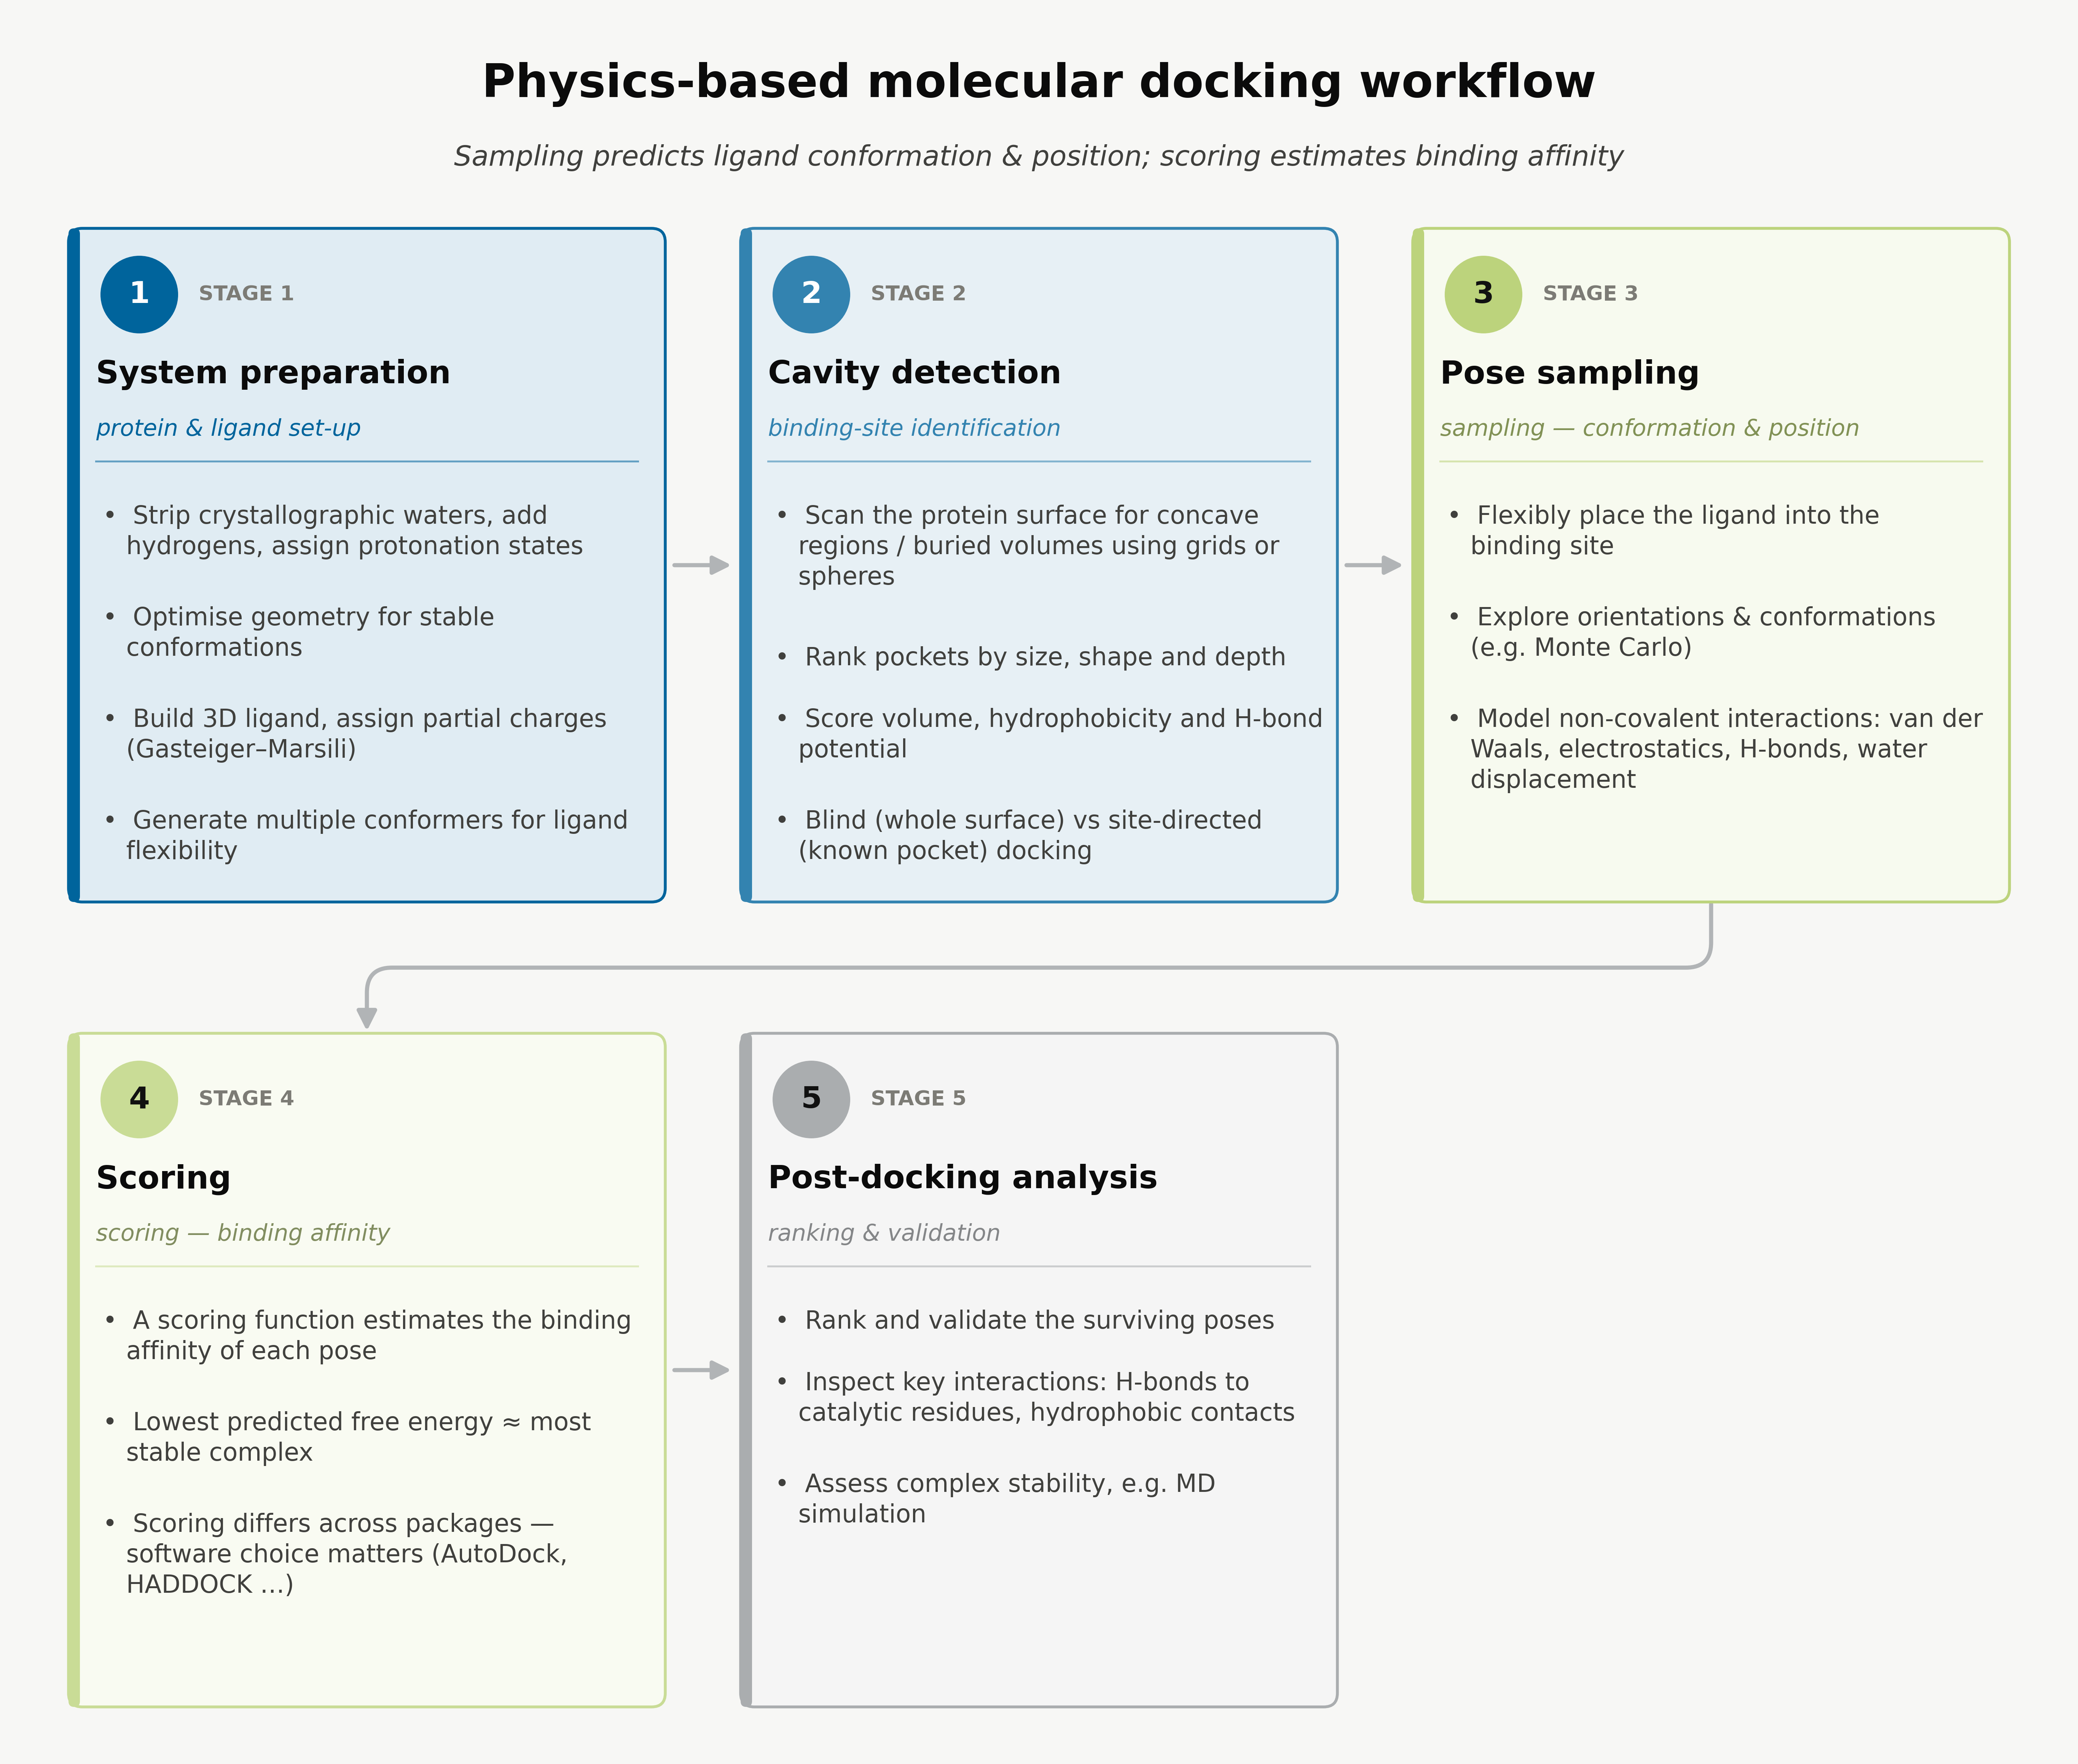
\includegraphics[width=\linewidth,height=0.78\textheight,keepaspectratio]{media/media/image1.png}
\caption[Physics-based docking flow chart]{Physics-based Docking Flow Chart. The figure is an original synthesis drawn by the author from the workflows described in \cite{ref015}, \cite{ref017}, \cite{ref018}, \cite{ref019}, \cite{ref020} and \cite{ref021}, and is neither reproduced nor adapted from any single source}\label{fig:literature-docking-workflow}
\end{figure}


\hypertarget{vina-scoring-function}{%
\subsection{Scoring Function}\label{vina-scoring-function}}

The Vina score ranks candidate poses as a weighted sum of distance-dependent interaction terms. The sum runs over every pair of atoms that can move relative to one another and normally excludes pairs separated by three or fewer consecutive covalent bonds \cite[p.~2]{ref022}:

\begin{equation}
c\  = \ \sum_{i\  < \ j}^{}{f_{t_{i}t_{j}}\left( r_{ij} \right)}
\label{eq:vina-1}
\end{equation}

Atom i carries a type t\textsubscript{i}. The function f depends not on the raw interatomic distance r\_ij but on the surface distance d\_ij = r\_ij \ensuremath{-} R\_ti \ensuremath{-} R\_tj, obtained by subtracting the two atoms\textquotesingle{} van der Waals radii. A value of d = 0 is van der Waals contact, negative values indicate steric overlap and positive values a gap between the surfaces. Hydrogen atoms are implicit and all interactions are truncated at 8\angstrom{}. The sum separates into an intermolecular and an intramolecular part, and the predicted affinity is read from the intermolecular part of the lowest-scoring conformation.

Three steric terms act on every atom pair, namely two attractive Gaussians and a repulsive parabola:

\begin{equation}
{gauss}_{1}(d)\  = \ exp\left\lbrack - \left( \frac{d}{0.5\angstrom{}} \right)^{2} \right\rbrack,\qquad
{gauss}_{2}(d)\  = \ exp\left\lbrack - \left( \frac{(d\  - \ 3\angstrom{})}{2\angstrom{}} \right)^{2} \right\rbrack
\label{eq:vina-2}
\end{equation}

The repulsion term completes them, equal to d\textsuperscript{2} for d \textless{} 0 and 0 otherwise. The two Gaussians reward contacts at and just beyond van der Waals distance while the repulsion penalises interpenetration. Together the three reproduce a Lennard-Jones shape without its hard singularity. Two further terms act only on suitable atom types. The hydrophobic term is piecewise linear, equal to 1 below a surface distance of 0.5\angstrom{} and 0 above 1.5\angstrom{}. The hydrogen-bond term is likewise piecewise linear, equal to 1 below \ensuremath{-}0.7\angstrom{} and 0 above 0. The intermolecular total is then rescaled by the number of active rotatable bonds N\_rot between heavy atoms in the ligand. This flexibility penalty down-weights ligands that pay a larger conformational-entropy cost on binding:

\begin{equation}
g\left( c_{inter} \right)\  = \ \frac{c_{inter}}{\left( 1\  + \ w \cdot N_{rot} \right)}
\label{eq:vina-5}
\end{equation}

The six weights were tuned once against the PDBbind dataset rather than derived from first principles. They take the values \ensuremath{-}0.0356 for gauss\textsubscript{1}, \ensuremath{-}0.00516 for gauss\textsubscript{2}, 0.840 for repulsion, \ensuremath{-}0.0351 for the hydrophobic term, \ensuremath{-}0.587 for hydrogen bonding and 0.0585 for N\_rot \cite{ref022}. Vina is therefore a fast and well-behaved surrogate objective rather than a physical free-energy decomposition.

Vinardo, short for Vina RaDii Optimized, reparametrises this function within the same program and additionally re-optimises the atomic radii \cite{ref023}, \cite{ref073}. Three changes separate it from the function above. It drops the second, longer-range Gaussian outright, so one steric-attraction term remains. That term is widened, and the hydrophobic and hydrogen-bond ramps are redrawn. The retained Gaussian is

\begin{equation}
{gauss}(d)\  = \ exp\left\lbrack - \left( \frac{d}{0.8\angstrom{}} \right)^{2} \right\rbrack
\label{eq:vinardo-1}
\end{equation}

against a width of 0.5\angstrom{} for the first Vina Gaussian. The repulsion term is unchanged in form, equal to d\textsuperscript{2} for d \textless{} 0 and 0 otherwise. The hydrophobic term is piecewise linear, equal to 1 below a surface distance of 0\angstrom{} and 0 above 2.5\angstrom{}, where Vina ramps between 0.5 and 1.5\angstrom{}. The hydrogen-bond term is likewise piecewise linear, equal to 1 below \ensuremath{-}0.6\angstrom{} and 0 above 0, against \ensuremath{-}0.7\angstrom{} for Vina. All terms are truncated at 8\angstrom{} as before, and the conformational-entropy correction of Equation~\ref{eq:vina-5} is carried over unchanged with the same N\_rot weight.

The four intermolecular weights are \ensuremath{-}0.045 for the Gaussian, 0.800 for repulsion, \ensuremath{-}0.035 for the hydrophobic term and \ensuremath{-}0.600 for hydrogen bonding, against \ensuremath{-}0.0356, 0.840, \ensuremath{-}0.0351 and \ensuremath{-}0.587 for the corresponding Vina terms, with the Vina gauss\textsubscript{2} weight of \ensuremath{-}0.00516 having no Vinardo counterpart. The re-optimised radii move the three commonest heavy-atom types and leave the rest alone. Carbon grows from 1.9 to 2.0\angstrom{}, nitrogen falls from 1.8 to 1.7\angstrom{} and oxygen from 1.7 to 1.6\angstrom{}, while sulfur, phosphorus and the halogens keep their Vina values. Because d is the surface distance, a radius change shifts every term that reads it, which is why the reparametrisation cannot be reduced to the weights alone.\footnote{These values were read from the source of the patched Vina build named at the head of Appendix~\ref{docking-protocols} rather than transcribed from the publication, so they are the parameters the reported Vinardo runs actually minimised.} Its published advantage was established on site-specific redocking and virtual screening \cite{ref073}, \cite{ref083}, and it does not transfer to the blind whole-protein search used here. Matched Vinardo passes place a rank-1 pose within 2\angstrom{} of the crystal ligand for 37 of the 303 complexes against 80 for Vina, and for 42 against 90 once each family is rescored with gnina. Those four counts are gated on distance alone, so they run above the validity-aware recovery figures reported elsewhere. They are also internal to the Meeko-ligand tree at exhaustiveness 32, matched to each other but not to the calibration arms the Results report, which are prepared end to end with ADFRsuite and searched at exhaustiveness 128. The contrast therefore settles the choice of scoring function and nothing else. Vina scoring underlies the reported results, and no Vinardo arm is carried into the calibration chapter.

\hypertarget{ai-based-molecular-docking-1}{%
\section{AI-Based Molecular Docking}\label{ai-based-molecular-docking-1}}

AI-based molecular docking tools employ diverse computational strategies. Some are deep-learning neural networks that predict binding poses directly from protein and ligand structures. Diffusion models like DiffDock \cite{ref024} treat docking as a generative sampling problem. Geometric deep learning approaches include EquiBind \cite{ref009}, \cite{ref010}, which predicts the bound pose directly with an SE(3)-equivariant network. TankBind \cite{ref025}, \cite{ref026} also encodes the protein with an equivariant network, but it predicts an inter-molecular distance map through a trigonometry module and then derives coordinates from it by optimisation. Regression-based models like KarmaDock \cite{ref027} and GAABind \cite{ref028} predict binding affinities or poses with learned scoring functions. Other notable AI-based algorithms include SurfDock, DiffBindFR, DynamicBind, QuickBind, and hybrid methods like Interformer, which integrate traditional conformational searches with AI-driven scoring functions. These tools also differ in the search space they require. DiffDock, EquiBind and TankBind need no user-specified binding site and localise the ligand themselves, whereas DeepDock and Uni-Mol must be given a pocket definition \cite{ref012}, \cite{ref035}. Co-folding models likewise require no predefined site, and they predict protein and ligand structure jointly rather than placing a ligand into a fixed receptor structure \cite{ref012}.

Independent comparative docking evaluations are summarised in Table~\ref{tab:literature-comparisons}, which is referenced from the Motivation. Three of them set physics-based methods against AI-based ones. Schaller et al. instead compare a physics-based docking program with two strategies guided by a co-crystallised ligand, deliberately excluding machine-learning docking methods because their training sets overlap the benchmark. That study therefore supplies the classical reference point rather than an AI comparison.

\begingroup\footnotesize
\begin{longtable}[]{@{}
  >{\raggedright\arraybackslash}p{(\columnwidth - 6\tabcolsep) * \real{0.1041}}
  >{\raggedright\arraybackslash}p{(\columnwidth - 6\tabcolsep) * \real{0.3676}}
  >{\raggedright\arraybackslash}p{(\columnwidth - 6\tabcolsep) * \real{0.2287}}
  >{\raggedright\arraybackslash}p{(\columnwidth - 6\tabcolsep) * \real{0.2996}}@{}}
\caption[Physics-Based and AI-Based Docking Studies]{Physics-Based and AI-Based Docking Studies}\label{tab:literature-comparisons}\tabularnewline
\toprule\noalign{}
{\raggedright \textbf{Study (Year)}} & \centering\arraybackslash\textbf{Docking Tools Compared} & \centering\arraybackslash\textbf{Datasets Used} & \centering\arraybackslash\textbf{Metrics for Comparison} \\
\midrule\noalign{}
\endfirsthead
\caption[]{Physics-Based and AI-Based Docking Studies (continued)}\tabularnewline

\toprule\noalign{}
{\raggedright \textbf{Study (Year)}} & \centering\arraybackslash\textbf{Docking Tools Compared} & \centering\arraybackslash\textbf{Datasets Used} & \centering\arraybackslash\textbf{Metrics for Comparison} \\
\midrule\noalign{}
\endhead
\bottomrule\noalign{}
\endlastfoot
Li et al. (2025) \cite{ref013} & Glide SP, AutoDock Vina (physics-based); SurfDock, DiffBindFR, DynamicBind (generative diffusion); KarmaDock, GAABind, QuickBind (regression-based AI); Interformer (hybrid) & Astex Diverse Set, PoseBusters Benchmark, DockGen (pose/validity); DEKOIS2.0, DUD-E (virtual screening) & RMSD (pose accuracy), PB-valid (physical plausibility), Interaction Recovery, ROC-AUC, EF0.5\%, BEDROC (VS), Generalisation (protein/ligand/pocket similarity) \\
Jiang et al. (2026) \cite{ref012} & Glide, AutoDock Vina, MOE, Discovery Studio, gnina (physics-based); Uni-Mol Docking V2, DiffDock, SurfDock, Interformer, EquiBind, FABind, DeepDock, TankBind (AI); AlphaFold3, Boltz-1, Chai-1 (AI co-folding) & PoseX-SD (self-docking), PoseX-CD (cross-docking), Astex & RMSD, Success Rate, Physical Validity, Generalisation, Leaderboard Ranking \\
Gu et al. (2025) \cite{ref032} & Glide, Surflex, rDock, LeDock (physics-based); CarsiDock, KarmaDock, DiffDock, FlexPose (AI-powered docking); RTMScore, EquiScore (AI rescoring) & VSDS-vd benchmark (TrueDecoy, TrueDecoy\textsubscript{gap}, RandomDecoy, MassiveDecoy) & RMSD (pose accuracy), PB-valid (physical plausibility), combined RMSD-and-PB-valid criterion, EF0.5\%, EF1\%, EF5\% (VS enrichment) \\
Schaller et al. (2024) \cite{ref033} & Fred (physics-based docking); Hybrid, Posit (guided by a co-crystallised ligand), all OpenEye Toolkits & 589 KLIFS kinase structures with 423 ATP-competitive ligands (cross-docking) & Heavy-atom RMSD (pose accuracy), bootstrapped success rate at 2\angstrom{}, Chemgauss4 and Posit probability scores \\
\end{longtable}
\endgroup

\hypertarget{diffdock-1}{%
\subsection{DiffDock}\label{diffdock-1}}

The graph representation behind the summary in the Literature Review is the following. Protein and ligand nodes encode chemical identity and geometry while edges encode connectivity or spatial neighbourhood, and the pose is parameterised by translation, rotation and internal torsion angles \cite{ref024}. Docking therefore becomes a prediction over the full space of rigid-body placement and conformational flexibility. The forward diffusion of training adds noise to those same variables, and the reverse process at inference predicts translation, rotation and torsion updates at each denoising step.

Two design choices follow from the multimodal nature of docking. Regressing a single pose can collapse several valid solutions into a physically meaningless average, whereas a diffusion model can represent the distribution itself. Sampling alone does not guarantee that the best pose is drawn first, which is why the authors added a separate confidence network that scores each generated complex for whether it falls below a conventional threshold such as 2\angstrom{} from the reference. The diffusion score model plays no part in that ranking. It predicts the gradient of the log-probability density over poses at each noise level and thereby steers the denoising trajectory rather than estimating an affinity.

The criteria that judge poses are consequently held implicitly in the network weights and the training objective rather than as chemically interpretable constants \cite{ref024}. Later work extended the framework toward flexible-pocket docking. DiffDock-Pocket adds receptor side-chain flexibility \cite{ref030}, and related diffusion models pack side chains during docking \cite{ref031}. Hybrid schemes pair diffusion-based pose generation with classical physics-based rescoring \cite{ref064}.

\hypertarget{equibind-1}{%
\subsection{EquiBind}\label{equibind-1}}

The single forward pass summarised in the Literature Review comprises five stages, namely graph construction, joint equivariant message passing, key-point prediction, rigid alignment and torsional refinement. The released implementation executes that sequence \cite{ref009}. Its central innovation is the third and fourth of those stages. EquiBind predicts matching sets of key points on the ligand and on the protein surface, then computes the rigid-body transformation that best aligns the two sets, typically through a singular-value-decomposition (Kabsch-style) step \cite{ref010}, \cite{ref062}. That transformation places the ligand into the predicted pocket in one operation, and a final conformer-fitting stage adjusts internal torsions to improve local geometry while keeping the ligand chemically valid \cite{ref009}, \cite{ref010}.

The training signals are ligand RMSD-type coordinate losses, rigid-body alignment losses and auxiliary terms that push the predicted placement toward the correct region of the protein \cite{ref010}. These objectives are the metrics of docking evaluation themselves, chiefly ligand RMSD and centroid distance. EquiBind therefore learns which placements are good because they minimise structural discrepancy to known complexes rather than because they minimise an analytic energy. It is neither a classical scoring-based method nor an uncertainty-aware sampler like DiffDock. The authors justified the design by arguing that a sufficiently expressive SE(3)-equivariant model can learn the necessary interaction patterns from structural examples alone \cite{ref010}. Later analyses show that highly flexible ligands and subtle local interactions still benefit from optional physics-based refinement, which keeps hybrid pipelines relevant in practice \cite{ref035}.

\hypertarget{optimization-tools-1}{%
\section{Optimisation Tools}\label{optimization-tools-1}}

\hypertarget{smina-1}{%
\subsection{smina}\label{smina-1}}

smina keeps Vina\textquotesingle s default empirical scoring function and its global search \cite{ref055}. It makes the individual energy terms available in parameterised form. The user can therefore reweight or replace each term and define custom atom types \cite{ref055}, \cite{ref057}. The energy it optimises is the function detailed in Section~\ref{vina-scoring-function}. The local minimisation was rebuilt rather than inherited \cite{ref057}. A smina-minimised geometry therefore need not coincide with the one stock Vina would return. In the fast local-minimisation mode used here, a pose seated in roughly the correct pocket but clashing sterically with the receptor is relaxed into the nearest minimum of that function, which removes the clash while leaving the placement essentially unchanged. Its source code is maintained on SourceForge and mirrored on GitHub \cite{ref057}.

\hypertarget{gnina-1}{%
\subsection{gnina}\label{gnina-1}}

The search gnina inherits from Vina through smina works as follows \cite{ref022}, \cite{ref056}, \cite{ref067}. A set of Markov chain Monte Carlo chains repeatedly applies random perturbations inside the search box, namely rigid-body translation and rotation of the whole ligand together with rotations about its rotatable bonds. Every candidate a chain generates is driven to a local minimum of the Vina function by gradient-based quasi-Newton minimisation, and a Metropolis criterion then decides whether that minimised pose is accepted as the next state of the chain.

The convolutional ensemble summarised in the Literature Review is built from two architectures, a linear five-convolutional-layer network (``Default2018'') and a twelve-layer densely connected network (``Dense''), because ensembling consistently yields better-ranked poses than any single network. Beyond CNNscore and CNNaffinity the program exposes their product CNN\_VS, proposed for virtual screening \cite{ref083} and used to rank compounds in a later prospective campaign \cite{ref068}. gnina 1.3, the version used here, retrains the models on the updated CrossDocked2020 v1.3 dataset, ports the deep-learning backend from Caffe to PyTorch for faster processor inference, compresses a five-member ensemble into a single ``fast'' student model by knowledge distillation and adds covalent-docking support \cite{ref067}. The tool therefore occupies a hybrid position, namely a physics-based sampler coupled to a deep-learning scoring function, and can serve either as a standalone docking program or, as here, purely as a rescoring and local-optimisation step applied to poses produced elsewhere. It is openly available on GitHub \cite{ref058}.

The training data matter for how the rescoring should be read. The gnina CNNs are trained on the CrossDocked2020 set \cite{ref059}, millions of poses obtained by cross-docking ligands into structurally similar Protein Data Bank pockets available up to 2020 \cite{ref056}. The calibration benchmark used here is restricted to complexes released from 2021 onwards, which is what its authors rely on to keep it clear of the PDBbind General Set v2020 that trained many of the methods they evaluated \cite{ref035}. Its receptor-ligand pairs are therefore absent from gnina\textquotesingle s training data as direct entries. That makes the rescoring a direct-entry temporal holdout rather than a similarity-controlled test, because a later release date does not exclude homologous proteins, familiar pockets, related ligands or templates (see Section~\ref{generalisation-in-the-context-of-current-literature}).

\hypertarget{docking-protocols}{%
\chapter{Docking Protocols}\label{docking-protocols}}

The three end-to-end pipelines share the same downstream validity definitions but differ in receptor preparation and conformer generation. AutoDock Vina and DiffDock receive the same RDKit \cite{ref086} ETKDGv3 + UFF start conformer, whereas EquiBind generates thirty ETKDGv3 + MMFF conformers. In the primary benchmark arms AutoDock Vina, DiffDock and unguided EquiBind all search the whole receptor without a crystal-derived restriction, so none is told where the ligand belongs. The separately reported EquiBind variants receive an fpocket- or P2Rank-predicted pocket and crop locally around it, and are set out in Section~\ref{equibind-pocket-guided}. The benchmark is therefore a comparison of deployed workflows rather than a controlled estimate of algorithm class alone. Tool-specific settings and pose budgets are summarised in Table~\ref{tab:appendix-protocols}, and the corresponding settings for the two Orai1 panels in Table~\ref{tab:appendix-orai-protocols}.

Five preparation choices are recorded here because they cannot be recovered from the output files. Every ligand entered preparation in the tautomer and the ionisation state its source file carried, and no protomer or tautomer enumeration and no pK\textsubscript{a} model ran on any ligand at any stage. The AutoDock ligand path does not preserve that hydrogen set. Each start conformer is converted to MOL2 with Open Babel and passed to \texttt{prepare\_ligand -A hydrogens}, whose valence-based repair builds hydrogens the source file does not carry. It adds 353 such atoms across 161 of the 308 benchmark ligands, 352 of them on nitrogen, and the docked poses carry them. The heavy-atom conformer is identical to the source file in all 308 cases, so the searched geometry is the shared start conformer while its hydrogen-bond donor set is not. Of the 308 benchmark start conformers 299 carry a net formal charge of zero, seven carry +1, one carries +2 and one carries \ensuremath{-}2, and all three Orai1 modulators were docked neutral in every reported arm. The ADFRsuite preparation described below assigns Gasteiger partial charges to both the ligand and the AutoDock receptor, and both sets are written into the PDBQT files. Neither the Vina nor the Vinardo function carries a charge-dependent term, since electrostatics and charge-dependent desolvation enter only through the AutoDock4 function that this study never invokes, so those charges never reached the objective that placed or minimised a reported pose. No atom record in any of the 308 benchmark receptors or the four Orai1 frames carries an alternate-location indicator, because the distribution already reduces each atom to a single conformer, so no alternate-conformation rule was applied here. The deposited fractional occupancy survives as a label on 2.1\% of benchmark receptor atoms across 258 of the 308 files. The AutoDock cleaning discards that label and writes every standard-residue atom at unit occupancy, five atoms of two modified residues excepted, and no step of any arm weights or filters on it. Crystallographic water is absent from the distribution itself, so every arm docks a water-free receptor whatever its cleaning step removes. The benchmark ships one coordinate file per entry carrying a crystallographic cell record and no assembly annotation, and that file was docked as supplied, so no biological assembly was generated and no symmetry mate was added. Its authors had already withdrawn the entries whose ligand contacts a symmetry mate, as Appendix~\ref{dataset} records. EquiBind shares none of that receptor path. It passes each receptor through \texttt{reduce} 4.15.250408, which adds hydrogens and optimises rotatable hydroxyl and ammonium orientations without its amide and histidine flip search, and 7WCF\_ACP carries no such stamp and was passed on byte-identical to the deposited file. Nothing is stripped and no partial charge is assigned, so the EquiBind receptors keep the deposited heteroatom records of 274 of the 308 entries and reach the validity screen with all-atom hydrogens. Their histidines are not on the AutoDock protonation model either, since \texttt{reduce} leaves both imidazole nitrogens bare on 3,898 of the 4,844 intact rings.

All software versions were verified by invoking each binary. Docking used AutoDock Vina v1.2.7-20-g93cdc3d-mod, a locally patched build rather than stock 1.2.7, DiffDock-L (PyTorch 2.4.0 / CUDA 12.4) and a custom EquiBind pipeline (February 2025, PyTorch 2.4.1 / CUDA 12.4). Local optimisation used gnina 1.3.2 and smina (9 November 2017 build, on the Vina 1.1.2 scoring base). PDBQT preparation used ADFRsuite 1.0 \cite{ref089}, whose \texttt{prepare\_ligand} and \texttt{prepare\_receptor} wrap its own bundled copies of the AutoDockTools \cite{ref049} \texttt{prepare\_ligand4.py} and \texttt{prepare\_receptor4.py} utilities, for both ligands and receptors of every AutoDock arm reported here, the benchmark and the Orai1 panels alike, with receptor cleaning by PDBFixer 1.12.0 on OpenMM 8.3.1. Meeko 0.7.1 \cite{ref087} prepared an earlier benchmark arm and the Vinardo tree, neither of which is carried into the reported calibration or Orai1 results. Open Babel \cite{ref088} was installed as version 3.1.1 although the binary reports 3.1.0. Blind pocket detection for EquiBind used fpocket 4.0 \cite{ref060} and P2Rank 2.5 \cite{ref061}. Physical-validity and interaction screening used PoseBusters 0.6.3 \cite{ref035} and PandaMap 4.1.0 \cite{ref090}. All screening, statistics and figure generation ran in one conda environment holding Python 3.12.12, RDKit 2025.09.1 (distributed as 2025.9.1), NumPy 2.3.4, SciPy 1.16.2, pandas 2.3.3 and scikit-learn 1.8.0. The RDKit release matters for interpretation. Its distance-geometry bounds define the bond-length and bond-angle tolerances, and its UFF implementation supplies both the pose energy and the reference ensemble of the internal-energy ratio. Most PoseBusters verdicts are tied to this exact version.

The docking binary is not stock either. AutoDock Vina was rebuilt from commit 93cdc3d of the upstream development branch with a local patch that adds boron as an atom type, which is what the \texttt{-mod} suffix in the version string above records. Stock Vina defines no boron atom type at any of its three typing levels. The patch is purely additive. It introduces one element type, one AutoDock type and one X-Score type, gives boron a van der Waals radius of 1.92\angstrom{} and a well depth of 0.29773 kcal/mol in the AutoDock parameter table, and takes the solvation parameter of carbon as an approximation. The well depth was chosen for this build rather than taken from a published parameter set. No existing atom\textquotesingle s parameters were altered, no scoring weight was touched and the search is unchanged. The three levels are chained, so the AutoDock type maps to the new element type and that element type to the new X-Score type, which carries a radius of 1.87\angstrom{} in both the Vina and the Vinardo radius sets. Boron is registered as a non-hydrophobic type that is neither a hydrogen-bond donor nor an acceptor, so it would enter the steric terms alone. The well depth is read only by the AutoDock4 scoring function, which this study never invokes.

The patch nevertheless bears on no number reported in this thesis, and the reason is recorded here rather than left to be discovered. None of the benchmark ligands carries boron. The one boron-bearing compound in this work is 2-APB, and it was converted to PDBQT with its boron carried as an aliphatic carbon rather than as the new type. Every docked 2-APB file in the study records the atom types A, C, HD, NA and OA and not one records B. The boron of 2-APB was therefore searched with the radius and the hydrophobicity of a carbon bonded to a heteroatom, and the added type stayed latent throughout. The steric consequence is small, since the aliphatic-carbon X-Score radius the atom was given is 1.9\angstrom{} under Vina and 2.0\angstrom{} under Vinardo against the 1.87\angstrom{} the new type would have supplied, and the Lewis acidity of the boron centre is unmodelled, as it would be under any empirical scoring function of this family.

The PoseBusters installation is not stock. One statement in \texttt{posebusters/modules/energy\_ratio.py} was patched locally. The exception handler guarding the UFF parameter check now logs the caught exception itself rather than indexing its second argument. As shipped, that handler also catches the assertion raised when UFF has no parameters for the ligand. That assertion carries only one argument, so the handler raises an \texttt{IndexError} of its own and aborts the entire \texttt{bust()} call instead of returning the empty result the module defines for a failed check. Every pose of a ligand that UFF cannot parameterise, for example one carrying hypervalent sulfur, a phosphate group or a coordinated metal, would otherwise be discarded without an error being reported. The patch adds no check, changes no threshold and alters no pass criterion. A second, purely operational override forces the conformer generation of the same check onto one RDKit thread to keep parallel workers from oversubscribing the processor. This changes scheduling and not verdicts.

\hypertarget{autodock-vina-2}{%
\section{AutoDock Vina}\label{autodock-vina-2}}

AutoDock Vina \cite{ref022}, \cite{ref023} provides the classical reference. Receptors are cleaned with PDBFixer, which strips waters, ions, metals and cofactors and maps covalently modified residues onto their standard parents. The modifying atoms that this mapping drops are restored afterwards as uncharged heteroatom records. The ADFRsuite preparation named above then adds hydrogens and Gasteiger partial charges and writes the PDBQT. It is called as \texttt{prepare\_receptor -A hydrogens -U nphs\_lps\_waters\_nonstdres}, so non-polar hydrogens are merged into their carbons. Hydrogens are placed from valence and geometry alone. That step accepts no pH argument and performs no pK\textsubscript{a} estimate. The pH-based hydrogen placement PDBFixer offers is left disabled on this path. No benchmark receptor was therefore titrated at a nominal pH. A fallback to that placement exists for receptors the converter cannot hydrogenate, and it fired on the Orai1 Fr0 receptor alone (Appendix~\ref{orai1-receptor-model}). The resulting model is uniform across the cohort. Histidine is protonated on both ring nitrogens and is therefore cationic, in all 4,485 residues with an intact imidazole ring. Aspartate and glutamate keep bare carboxylates, lysine keeps a charged ammonium and arginine a charged guanidinium, and every serine, threonine and tyrosine hydroxyl carries its hydrogen. Cysteine is the exception, since the preparation builds no thiol hydrogen and the 316 of 2,282 cysteines that carry one inherited it from the deposited coordinates. Chain termini are taken as deposited and are not repaired, which leaves a charged amino terminus and a charged carboxy terminus wherever an OXT atom is present. Ligands use the shared start conformer. The whole-protein receptors are therefore apo-like rather than cofactor-retaining. Heteroatom records survive in only 28 of the 303 analysed receptors, and in 30 of the 308 prepared and are almost entirely covalently modified amino acids such as phosphoserine and carboxylated lysine. No haem, flavin, metal or ion is present in the docked structure even where the deposited entry carried one. The search box spans the whole receptor, so AutoDock searches blindly exactly as DiffDock does. Vina runs at energy range 6 kcal/mol and random seed 42, retaining up to thirty ranked modes per complex. Exhaustiveness is the one setting that was varied, and the reported arm is exhaustiveness 128.

A quarter of the benchmark carries a metal where the ligand binds, and the preparation removes it. In 78 of the 303 analysed entries a residue carrying a metal ion or a metal-containing cofactor has an atom within 5\angstrom{} of a heavy atom of the deposited reference instance of the ligand, most often magnesium, zinc or iron. Membership is a property of the complex and does not follow the copy a pose is scored against. One AutoDock rank-1 success, 7JHQ\_VAJ, is therefore metal-adjacent although it is scored against a copy with no metal within 39\angstrom{}, the reference instance carrying a sodium ion at 2.4\angstrom{}. No success of any selected variant runs the other way. Sixteen of the 78 involve a metal-bearing cofactor such as haem, an iron-sulfur cluster or cobalamin, and the remaining 62 involve a free ion. None survives preparation in the AutoDock or the DiffDock arm. Those 78 prepared AutoDock receptors retain only modified amino acids such as carboxylated lysine and phosphoserine, and the matching DiffDock receptors retain no heteroatom record at all, so the stripping does not favour either arm. EquiBind is the exception, because its preparation keeps the deposited heteroatom records and its receptors therefore keep their metals. The two strata are alike in ligand size. Median heavy-atom counts are 25 and 22.5 (Mann-Whitney U p = 0.124, Cliff\textquotesingle s \ensuremath{\delta} = +0.12), median rotatable-bond counts are 5 and 5 (p = 0.596, \ensuremath{\delta} = \ensuremath{-}0.04) and median molecular weights are 358 and 361~Da (p = 0.468, \ensuremath{\delta} = +0.06), with positive values meaning the metal-free stratum is larger. Recovery still differs, and it differs by stratum rather than by tool. Rank-1 recovery is 51.1\% for AutoDock and 49.3\% for DiffDock on the 225 metal-free complexes, against 43.6\% and 26.9\% on the 78 metal-adjacent ones. Both tools lose accuracy where a metal has been stripped, but DiffDock loses far more, so AutoDock leads on the metal-adjacent stratum while the two are level on the metal-free one. The paired top-15 contrast, taken as DiffDock minus AutoDock, is \ensuremath{-}8.4 percentage points on the metal-free stratum (141 against 160 of 225, exact McNemar p = 0.056) and \ensuremath{-}19.2 points on the metal-adjacent stratum (38 against 53 of 78, p = 0.028). The split was made after the fact, and the difference between the two stratum contrasts is itself unresolved (Fisher\textquotesingle s exact test on the discordant pairs p = 0.440), so the widening is reported as heterogeneity rather than as an established interaction. The failure diagnosis separates the tools rather than the strata. On the metal-free stratum 58.2\% of AutoDock and 70.2\% of DiffDock rank-1 failures hold no qualifying pose at any depth, and on the metal-adjacent stratum the shares are 56.8\% and 70.2\%. AutoDock\textquotesingle s rank-1 misses are therefore about as often recoverable deeper in its own list on either stratum, whereas DiffDock\textquotesingle s are more often absent from the pool altogether. The partition is insensitive to the distance criterion in direction if not in size, since a 4\angstrom{} rule classes 73 complexes as metal-adjacent and a 6\angstrom{} rule 81, with stratum contrasts of \ensuremath{-}9.1 and \ensuremath{-}17.8 points and of \ensuremath{-}8.1 and \ensuremath{-}19.8 points.

The whole receptor was searched so that AutoDock Vina faces the same problem as the two methods that localise the ligand themselves. The box is constructed per receptor rather than set to a fixed size. Its centre is the midpoint of the axis-aligned bounding box over every atom record of the prepared receptor, and each edge is that axis\textquotesingle s span plus 1\angstrom{} on either side. No further padding is applied, and every deposited copy of the ligand lies inside the box. Over the 303 analysed receptors the resulting edges run from 29.5 to 167.4\angstrom{} with a median of 63.5\angstrom{}, and the volumes from 44,430 to 2,479,703\angstrom{}\textsuperscript{3} with a median of 263,874\angstrom{}\textsuperscript{3}, a 56-fold range across the cohort. A box centred on the crystal ligand supplies part of the answer before the search begins, as it did in the benchmark this study calibrates against, which gave Vina a 25\angstrom{} cube centred on the crystal-ligand heavy atoms \cite{ref035}. That cube is 15,625\angstrom{}\textsuperscript{3}, so the median box used here is about seventeen times its volume and the largest about 159 times. Removing that information costs real accuracy, because a fixed number of Monte Carlo search runs is diluted over a much larger volume \cite{ref079}, \cite{ref080}, \cite{ref081}, and a whole-protein box has been reported to reduce Vina pose-prediction success on CASF-2016 \cite{ref084} to roughly a third to a half of the site-specific rate \cite{ref082}. That dilution is the reason exhaustiveness was treated as a variable here rather than left at its default, and Appendix~\ref{exhaustiveness-selection} shows how much of the loss raising it recovers. The AutoDock numbers reported here remain blind-docking numbers rather than re-docking numbers.

Eight AutoDock variants were run on this set, five independent docking passes at exhaustiveness 18, 32, 64, 92 and 128 under the default Vina function \cite{ref023}, plus a gnina rescoring pass over three of them. They are tabulated in Table~\ref{tab:appendix-exhaustiveness-ladder}, whose section sets out the basis for the choice, and the Results chapter prints the selected rung alone. The five passes share prepared ligands, receptors, box and seed, so exhaustiveness is the only variable and they are directly comparable. Each pass supplies the raw variant of its rung. The three rescored variants are not separate searches but post-hoc passes over the poses of a completed pass, using gnina 1.3.2 \cite{ref056}, \cite{ref067} in its rescoring mode. Exhaustiveness 18 and 92 were not rescored. Each pose is rebuilt to SDF from a bond-order template and processed individually in a box extended 4\angstrom{} around that pose, with a fixed seed of 42 and no crystallographic input. A Vinardo-scored pass \cite{ref073} exists on this dataset but is prepared from a different ligand converter, so it is not comparable with the arms above and is not reported in this chapter.

Three protocol details of the rescoring pass matter for interpretation. The gnina-side empirical objective is the Vina function, matching the function the poses were searched under. Ranking is taken from CNNaffinity rather than gnina\textquotesingle s default CNNscore ordering, with the original Vina rank retained alongside it. The convolutional model was pinned to the crossdock\_default2018 ensemble rather than left at the gnina 1.3 default. A fourth detail that matters elsewhere does not arise here. Because the ADFRsuite pose files carry no embedded SMILES, the raw poses are rebuilt from a template as heavy-atom records and the rescored ones are written back by gnina carrying polar hydrogens only, so neither arm reaches the check with the full hydrogen shell that produces the artefact, so the two arms reach the validity screen on the same hydrogen footing and the internal-energy artefact that separates a full-hydrogen raw arm from a polar-hydrogen rescored one does not apply.

The consequence of that ranking choice is quantified here, because the head is a further selection degree of freedom on top of exhaustiveness and rescoring. Ordering the rescored pose set by CNNaffinity recovers 149 of the 303 complexes at rank-1, or 49.2\%. Ordering the same poses by gnina\textquotesingle s default CNNscore recovers 152, or 50.2\%, and ordering them by the minimised Vina energy recovers 128, or 42.2\%. The two convolutional heads return a different rank-1 verdict on 31 complexes, 14 favouring CNNaffinity and 17 favouring CNNscore, and the paired contrast is not resolved (exact McNemar p = 0.720). The head in use therefore does not report the AutoDock arm at its most favourable rank-1 value, and the choice between the two convolutional heads is immaterial to every conclusion drawn from this arm. What does matter is that both convolutional heads beat the minimised empirical energy by seven to eight percentage points at rank-1. The effect is largely confined to the top of the ranking. At top-15 the three heads recover 213, 213 and 202 complexes, and at top-30 all three recover the same 214.

gnina is used on the AutoDock arm in its rescoring mode, so the CNN scores and re-orders the poses without driving their geometry. That is the mode the gnina authors recommend \cite{ref056}. A rescored arm shares its rung\textquotesingle s pose set exactly, so the two can be compared as paired observations, whereas two rungs are independent searches and share only their inputs.

\hypertarget{exhaustiveness-selection}{%
\section{Choice of Exhaustiveness and Rescoring}\label{exhaustiveness-selection}}

Vina spreads a fixed number of Monte Carlo runs over whatever volume it is given, so the whole-receptor boxes of Section~\ref{autodock-vina-2} make exhaustiveness a decision rather than a default. The five rungs described there were staged once from the base arm rather than re-derived per rung, and three of them were additionally rescored with gnina, giving the eight variants of Table~\ref{tab:appendix-exhaustiveness-ladder}. This section records why exhaustiveness 128 with gnina rescoring was selected and what the ladder implies about searching harder still.

Selection uses the top-15 ranking depth fixed in the Results. Table~\ref{tab:appendix-exhaustiveness-ladder} gives every arm at four depths on the validity-aware recovery gate, namely a pose that is PoseBusters-valid and within 2\angstrom{}. At top-15 the selected arm recovers 213 of 303 complexes and beats each of the seven alternatives on an exact McNemar test, with Holm-adjusted p-values running from 7.3e-20 against exhaustiveness 18 to 0.005 against its own raw search and against exhaustiveness 64 rescored. It leads strictly at every depth from rank-1 to top-25 and ties at top-26. At rank-1 six of the seven contrasts survive correction within this seven-contrast family. The one that does not is the contrast with exhaustiveness 64 rescored, where the arm leads nominally at 149 against 141 on 16 against 8 discordant complexes (exact p = 0.15) and the ordering is unresolved. Over the full thirty-pose pool the raw exhaustiveness-128 arm is nominally ahead, 217 against 214, because rescoring minimises poses and a few cross the threshold the wrong way. The selected arm is therefore the best configuration at every depth a user is likely to inspect, and the raw search overtakes it only over the whole pool. On the three-part endpoint the Results use for selection the same ordering holds, at 175 complexes against 166 for its own raw search and 110 at exhaustiveness 18, with Holm-adjusted p-values from 6.5e-18 to 0.023 over the same family. That family is the seven contrasts against the selected arm, and the steps over raw exhaustiveness 128 and over exhaustiveness 64 rescored are the two contrasts that would not survive a correction taken over all twenty-eight pairs of the ladder.

The two components are separately necessary. Holding rescoring fixed, raising exhaustiveness from 32 to 128 moves top-15 recovery from 170 to 213 complexes. Holding exhaustiveness fixed at 128, adding rescoring moves it from 198 to 213, gaining 19 complexes and losing 4. That gain is a ranking gain rather than a sampling one, since the rescored arm reorders the pool the raw arm produced rather than adding to it. Carried at the parent Vina order instead of the CNN-affinity order, the same rescored poses recover 129 complexes at rank-1 and 196 at top-15, below the raw search at 130 and 198, which places the whole of the advantage in the ranking head. Figure~\ref{fig:appendix-exh-rescored} shows it as a vertical step at each rung, widest at rank-1 and absent over the whole pool, and Figure~\ref{fig:appendix-exh-depth} resolves the same behaviour rung by rung against ranking depth.

\begin{figure}[!htbp]
\centering
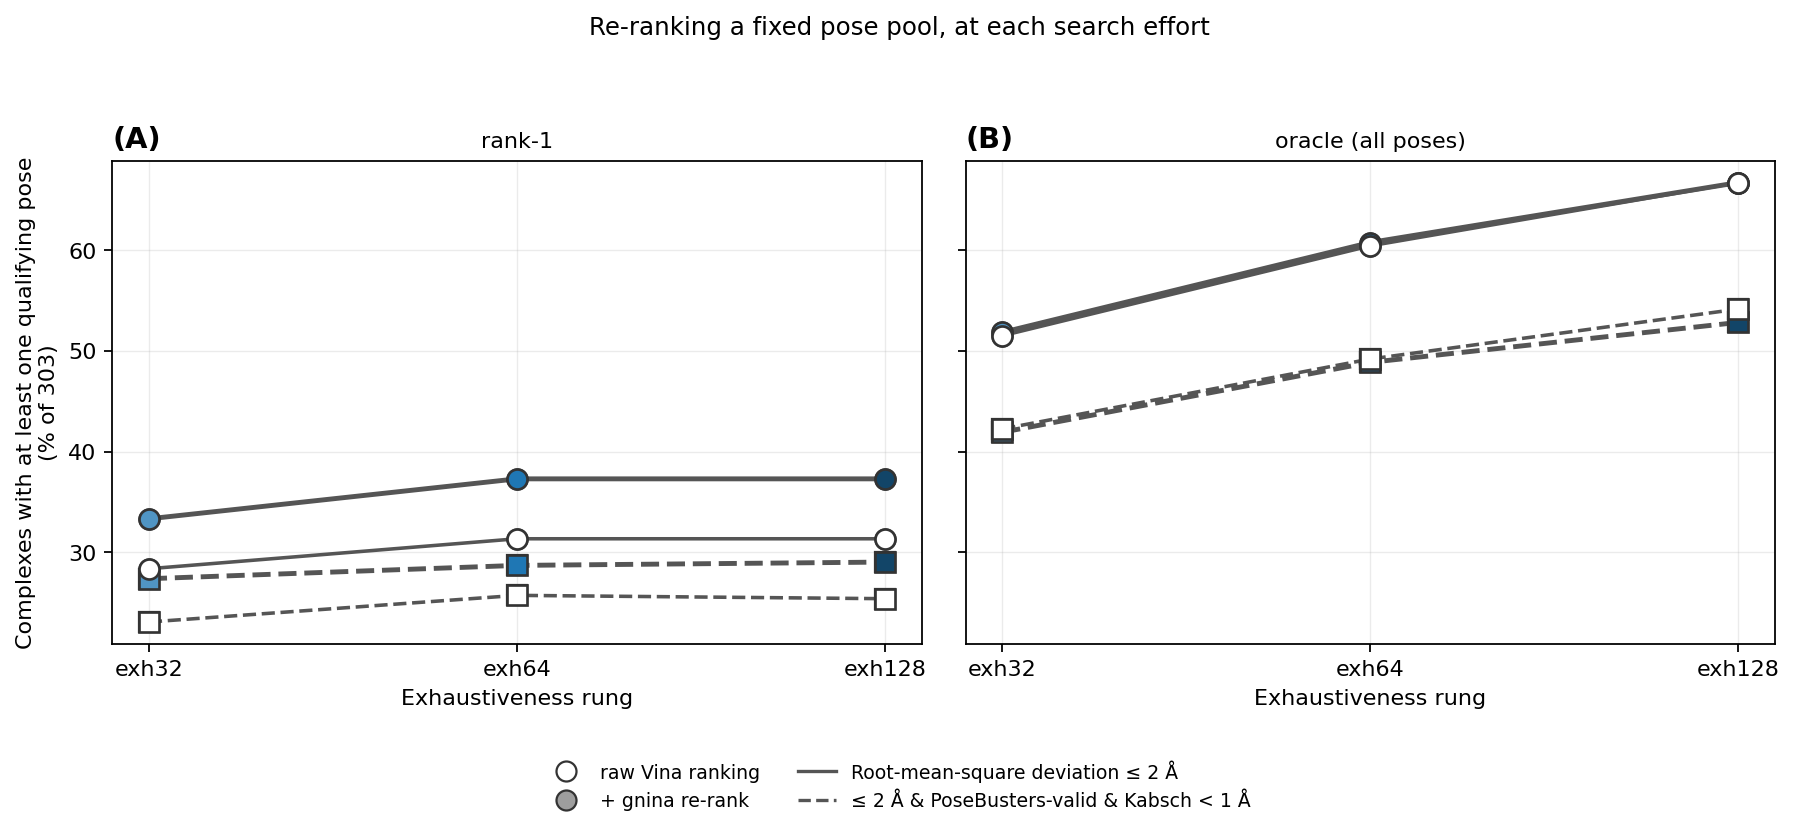
\includegraphics[width=\linewidth,height=0.44\textheight,keepaspectratio]{media/media/image44.png}
\caption[Raw Vina ranking against gnina re-ranking at each rung]{Raw Vina ranking against gnina re-ranking of the identical pose pool, at the three rescored rungs. Re-ranking buys at rank-1 (A) what more searching cannot, whereas over the whole pool (B) it gains nothing on placement and gives a little back on the three-part gate, because it reorders a pool rather than extending it}\label{fig:appendix-exh-rescored}
\end{figure}

\begin{figure}[!htbp]
\centering

\includegraphics[width=\linewidth,height=0.44\textheight,keepaspectratio]{media/media/image45.png}
\caption[What each rung of the ladder buys against ranking depth]{Complexes gained over the rung below, against the number of top-ranked poses inspected, on the near-nativeness gate (A) and on the three-part gate (B). Ringed markers carry an unadjusted McNemar p below 0.05. A rung\textquotesingle s verdict depends on how deep the user looks, and the top step is worth seven complexes at rank-1 on the near-nativeness gate, where it is already individually resolvable at an unadjusted p of 0.039, and six on the three-part gate, where it first resolves at depth 2}\label{fig:appendix-exh-depth}
\end{figure}

\begin{longtable}[]{@{}
  >{\raggedright\arraybackslash}p{(\columnwidth - 12\tabcolsep) * \real{0.3050}}
  >{\raggedleft\arraybackslash}p{(\columnwidth - 12\tabcolsep) * \real{0.1000}}
  >{\raggedleft\arraybackslash}p{(\columnwidth - 12\tabcolsep) * \real{0.1000}}
  >{\raggedleft\arraybackslash}p{(\columnwidth - 12\tabcolsep) * \real{0.1000}}
  >{\raggedleft\arraybackslash}p{(\columnwidth - 12\tabcolsep) * \real{0.1000}}
  >{\centering\arraybackslash}p{(\columnwidth - 12\tabcolsep) * \real{0.1450}}
  >{\raggedleft\arraybackslash}p{(\columnwidth - 12\tabcolsep) * \real{0.1350}}@{}}
\caption{AutoDock Exhaustiveness Ladder: Recovery by Ranking Depth and Search Cost}\label{tab:appendix-exhaustiveness-ladder}\tabularnewline
\toprule\noalign{}
{\raggedright \textbf{Variant}} & \centering\arraybackslash\textbf{Rank-1} & \centering\arraybackslash\textbf{Top-5} & \centering\arraybackslash\textbf{Top-15} & \centering\arraybackslash\textbf{All 30} & \centering\arraybackslash\textbf{p\textsubscript{Holm} vs selected} & \centering\arraybackslash\textbf{Search h} \\
\midrule\noalign{}
\endfirsthead
\caption[]{AutoDock Exhaustiveness Ladder: Recovery by Ranking Depth and Search Cost (continued)}\tabularnewline
\toprule\noalign{}
{\raggedright \textbf{Variant}} & \centering\arraybackslash\textbf{Rank-1} & \centering\arraybackslash\textbf{Top-5} & \centering\arraybackslash\textbf{Top-15} & \centering\arraybackslash\textbf{All 30} & \centering\arraybackslash\textbf{p\textsubscript{Holm} vs selected} & \centering\arraybackslash\textbf{Search h} \\
\midrule\noalign{}
\endhead
\bottomrule\noalign{}
\endlastfoot
Exhaustiveness 18 & 92 & 127 & 138 & 143 & 7.3e\ensuremath{-}20 & 2.14 \\
Exhaustiveness 32 & 109 & 147 & 161 & 170 & 1.4e\ensuremath{-}12 & 2.56 \\
\quad + gnina rescoring & 129 & 160 & 170 & 170 & 9.1e\ensuremath{-}09 & 2.56 \\
Exhaustiveness 64 & 123 & 162 & 190 & 201 & 1.4e\ensuremath{-}04 & 3.14 \\
\quad + gnina rescoring & 141 & 187 & 200 & 200 & 0.0052 & 3.14 \\
Exhaustiveness 92 & 123 & 164 & 194 & 209 & 9.3e\ensuremath{-}04 & 4.84 \\
Exhaustiveness 128 & 130 & 170 & 198 & 217 & 0.0052 & 4.73 \\
\quad + gnina, selected & 149 & 200 & 213 & 214 & --- & 4.73 \\
\multicolumn{7}{@{}p{\dimexpr\columnwidth-7\tabcolsep\relax}@{}}{\footnotesize%
Complexes of 303 with at least one pose that is PoseBusters-valid and within 2\angstrom{} of the nearest deposited copy of the ligand among the first d ranks. The significance column is an exact McNemar test of that arm against the selected arm at top-15, Holm-corrected across the family of seven. Search h is measured Vina wall time summed over the same 303 complexes, and is a property of the rung rather than of the rescoring, so a raw arm and its rescored sibling carry the same figure. The exhaustiveness-32 rung ran on twenty threads and the other four on thirty-two. The column is not monotone, exhaustiveness 92 measuring 0.110 hours more than the harder search at 128. That inversion is a property of how the machine was loaded on the day rather than of the setting, and the paragraphs below therefore treat the top step as carrying no measurable cost. Rescoring cost is not commensurable with search time and is reported for the selected rung in the Hardware and Timing Basis section below.} \\
\end{longtable}

The ladder buys progressively less, as Figures~\ref{fig:appendix-exh-cost} and \ref{fig:appendix-exh-return} show against measured search time. Read as complexes recovered per additional hour, on the conjunction of validity, near-nativeness and form over the whole pool, the three measurable steps return +71.6, +35.9 and +5.9 complexes per hour. The contrast between the first and last, recomputed on the same bootstrap-resampled complexes, is +65.6 per hour with a 95\% interval of +32.1 to +137.2. That interval lies wholly above zero, which is the diminishing-returns claim and the single cell fixed in advance for a confirmatory reading, every other cell here being descriptive. In absolute terms the five rungs recover 98, 128, 149, 159 and 164 complexes, so the first step adds thirty and the last adds five. Those counts and the confirmatory interval above are kept on the single deposited instance on which the cell was fixed in advance. Scored against the nearest deposited copy the same rungs recover 115, 143, 166, 172 and 178 complexes, so the first step adds twenty-eight and the last six, the three measurable steps return +66.8, +39.3 and +3.5 complexes per hour, and the first-to-last contrast is +62.4 per hour with a 95\% interval of +32.0 to +133.3.

\begin{figure}[!htbp]
\centering
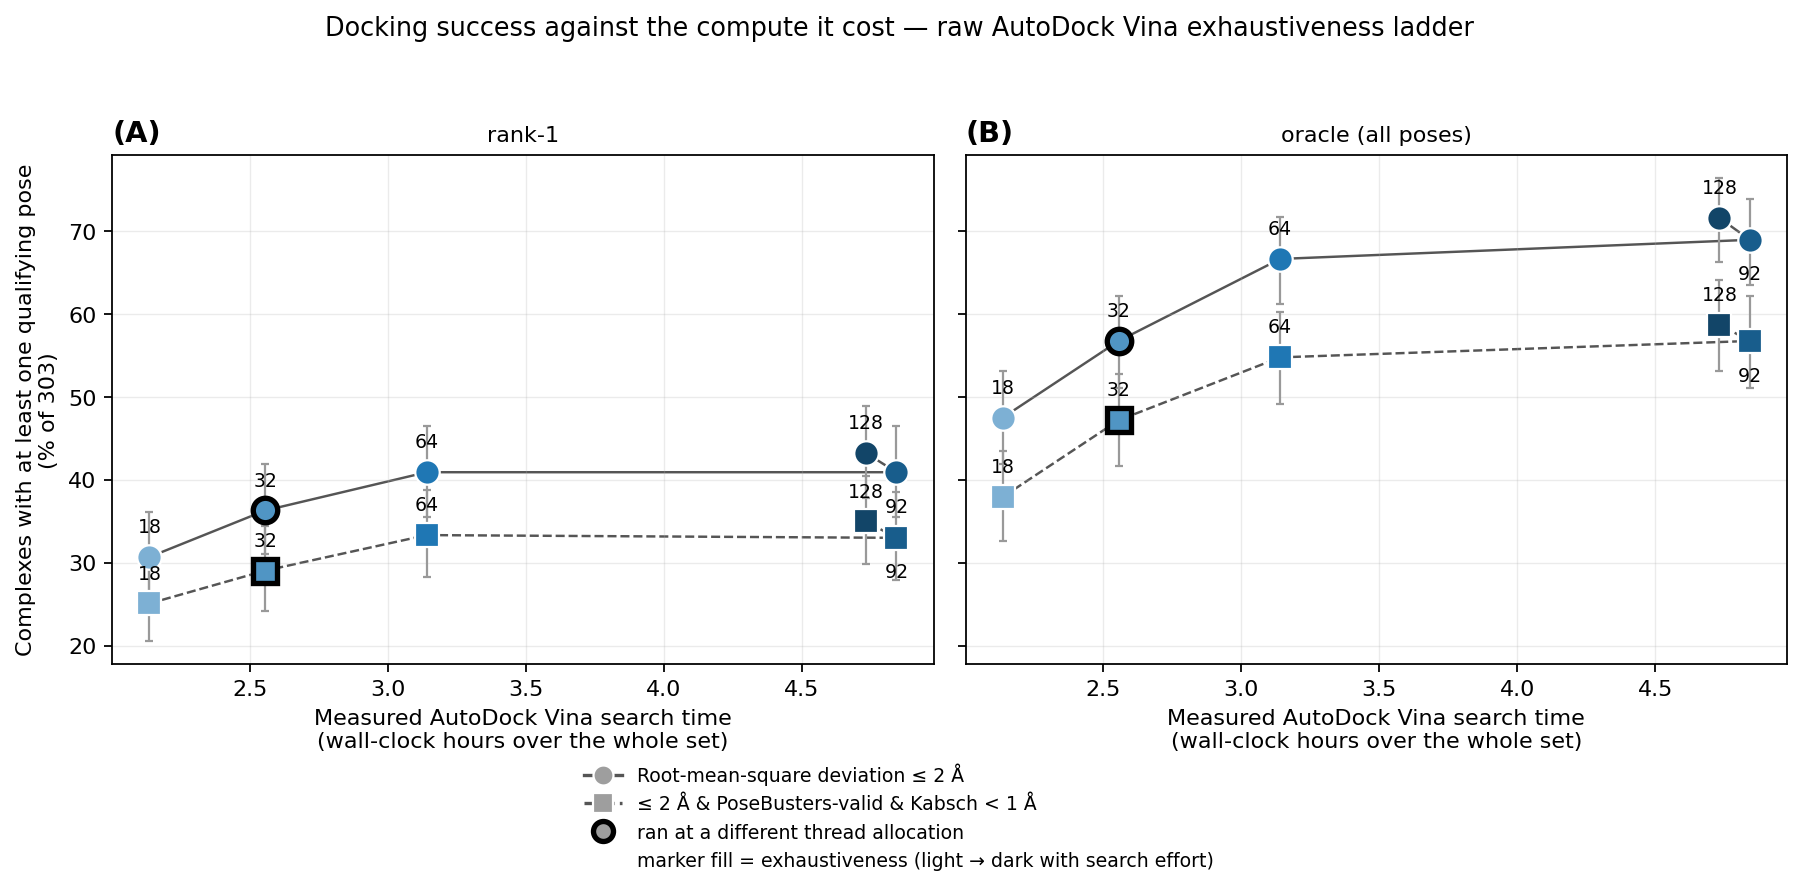
\includegraphics[width=\linewidth,height=0.44\textheight,keepaspectratio]{media/media/image46.png}
\caption[Docking success against the compute it cost]{Complexes with at least one qualifying pose against measured Vina search time, at rank-1 (A) and over the whole pool (B), with Wilson intervals. Marker fill runs light to dark with search effort and a ringed marker denotes the rung that ran at a different thread allocation. Exhaustiveness 92 is the most expensive rung on the ladder and buys nothing at rank-1}\label{fig:appendix-exh-cost}
\end{figure}

\begin{figure}[!htbp]
\centering

\includegraphics[width=\linewidth,height=0.44\textheight,keepaspectratio]{media/media/image47.png}
\caption[Marginal return per additional hour of search]{Additional complexes recovered per extra wall-clock hour for each step up the ladder, at rank-1 (A) and over the whole pool (B), with paired complex-level bootstrap whiskers. Hatching separates the two gates over the same rung colour. The top step carries no bar because its measured cost delta is negative, so no return per hour can be formed from it}\label{fig:appendix-exh-return}
\end{figure}

The fourth step resists a cost statement altogether. Exhaustiveness 92 to 128 adds six complexes over the pool and six at rank-1 when scored against the nearest deposited copy, but its measured wall-time delta is \ensuremath{-}0.110 hours, which is not a cost. Each arm is one unreplicated batch run on one day with no load telemetry, and the residual arm effect spans 18.7 percentage points, so the batch confound is the size of the treatment effect. That step is therefore too small to separate from the noise in how the machine was loaded, which is not the same as searching harder being free.

One thing follows, one follows in part, and a third does not. Returns diminish sharply and monotonically, the last measurable step costing about seventeen minutes of wall time per additional complex on the nearest-copy counts against about one minute for the first. The ceiling that remains is only partly a ranking ceiling. Measured on placement alone, without the validity requirement the ladder table imposes, raw rank-1 recovery is 124 complexes at exhaustiveness 64 and 92 and 131 at 128, while rescoring lifts the two rescored rungs to 144 and 151, so doubling the pool beneath the rescorer still adds seven complexes at rank-1. Extra sampling keeps finding poses that the empirical function fails to promote, and the rescorer promotes a part of what the harder search finds. What does not follow is that exhaustiveness above 128 is useless, because the ladder stops there and no measurement speaks beyond it.

One caveat applies to the selected arm itself. Choosing the best variant of a family on the same 303 complexes that then report its performance carries a winner\textquotesingle s curse. The selected arm\textquotesingle s recovery is therefore an optimistic estimate of what the same configuration would achieve on fresh complexes. The standard estimator scales the paired standard error of the winner\textquotesingle s margin over its runner-up by the expected maximum of k standard normals. Applied per family on the three-part selection endpoint at top-15, it puts the optimism at 0.4 percentage points for the two AutoDock arms at exhaustiveness 128, at 0.5 for the three DiffDock arms and at 1.0 for the three EquiBind arms. Taken over the eight-arm ladder of Table~\ref{tab:appendix-exhaustiveness-ladder} instead, the AutoDock correction rises to 1.1 points at top-15 and 1.5 at rank-1, and to 1.4 and 1.6 on the validity-aware gate of that table. The Limitations quote the per-family range. None of these corrections affects the ordering of the arms against one another, which is what this section claims, but each should be subtracted in spirit from any absolute figure carried forward.

\hypertarget{diffdock-2}{%
\section{DiffDock}\label{diffdock-2}}

DiffDock \cite{ref024}, \cite{ref008}, specifically DiffDock-L \cite{ref091}, is the diffusion-based generative method. It docks blindly over the whole receptor without a supplied search box. ESM2-650M embeddings represent the protein and the shared start conformer provides the ligand graph. Reverse diffusion uses twenty denoising steps and generates up to thirty candidates per complex, each ranked by native confidence. Refinement was attempted independently with both smina and gnina for every raw pose, and each refined variant contains 8,993 outputs from 9,013 raw poses, with failed outputs excluded. The main Results designate the smina-refined variant as DiffDock + smina, while Appendix optimisation and ranking diagnostics label raw and gnina-optimised variants explicitly. Both refiners were applied as a pure local minimisation, with the search restricted to a 4\angstrom{} box drawn around the pose being relaxed. Each refined copy is written beside its original and inherits that original\textquotesingle s confidence rank. A refined score is computed for every pose and written to the optimiser log, but it is never propagated into the per-pose analysis tables and never used to order poses. Refinement therefore moves coordinates and at no point re-orders the thirty candidates, and every DiffDock rank reported in this thesis is the confidence rank applied to refined geometry.

\hypertarget{equibind-2}{%
\section{EquiBind}\label{equibind-2}}

EquiBind \cite{ref010} is a direct-regression method that natively emits one pose. To create a comparable retrospective pool, this study docks thirty fixed RDKit ETKDGv3 conformers, minimised with MMFF, in unguided mode against the full uncropped receptor. That expansion is a custom pipeline rather than native EquiBind behaviour. Refinement was attempted independently with smina and gnina for every output. The unguided variants contain 9,090 smina outputs and 9,088 gnina outputs from 9,090 raw poses. Two gnina refinements, both of complex 7EPV\_FDA, produced no output and are the only refinement failures in this arm. The main Results use the unguided EquiBind + gnina variant. Two pocket-guided site modes were also run, each in the same three refiner states, and are reported in Section~\ref{equibind-pocket-guided} below.

The pipeline also implements an intermediate ligand-relaxation stage, in which each pose is minimised with the Universal Force Field against the receptor atoms within 6\angstrom{} of the ligand, for at most two hundred iterations and with every receptor atom held rigid. It was switched off for every run reported in this thesis, the calibration benchmark and both Orai1 panels alike, and the 308 committed benchmark run records confirm the setting. A minimisation that may move only the ligand cannot lift a buried pose out of a steric overlap and relieves the overlap by deforming the ligand instead. Neither refiner repairs that kind of damage, because smina and gnina move a pose only by rigid-body transformation and rotation about its rotatable bonds.

\hypertarget{equibind-pocket-guided}{%
\subsection{Pocket-Guided Variants}\label{equibind-pocket-guided}}

Six further configurations tested whether supplying an external site predictor improves this workflow. The receptor was cropped to an 11\angstrom{} shell around the predicted site, an 8\angstrom{} residue-selection radius plus a 3\angstrom{} margin, using fpocket 4.0 \cite{ref060} or P2Rank 2.5 \cite{ref061}, and each guided arm was then taken raw, smina-optimised and gnina-optimised exactly as the unguided one was. These arms hold binding-site information that neither AutoDock Vina nor DiffDock receives, so they can never enter the three-tool comparison. They are reported here because the answer they give is negative.

Guidance loses on every accuracy endpoint. On the three-part selection endpoint at the top-15 depth the unguided arms recover 2, 48 and 57 complexes of 303 taken raw, with smina and with gnina, against 0, 10 and 20 under fpocket and 0, 9 and 23 under P2Rank, so the best guided configuration trails the selected unguided one by 34 complexes. Near-native recovery over the full thirty-pose pool separates them the same way, at 19, 67 and 86 complexes unguided against 0, 19 and 32 and 1, 28 and 43, the fpocket raw arm recovering no near-native complex and the P2Rank raw arm one. The guided figures are those of the original local-search refinement, which was not repeated for them because the guided arms trail the unguided one on every endpoint and were not carried forward. Pooled physical validity follows, at 2.9\%, 51.3\% and 62.0\% unguided against 0.3\%, 15.2\% and 28.4\% and 0.6\%, 20.7\% and 38.0\%. The Form block is the exception and is flat, between 179 and 199 complexes across all nine configurations, so cropping the receptor moves where the ligand is put without changing its internal geometry.

One axis runs the other way and is stated rather than omitted. Counting complexes with at least one PoseBusters-valid pose anywhere in the pool, the optimised guided arms lead, at 261 for fpocket with gnina and 282 for P2Rank with gnina against 266 unguided. Guidance therefore raises the chance that some admissible pose exists while collapsing the share of poses that are admissible and losing the placement outright, which is the combination a selection endpoint requiring validity, placement and form together is built to catch. The P2Rank arms also rest on a narrower pose base. Every complex is represented, but the detector returned fewer than three pockets on 38 of them, nineteen contributing ten poses and nineteen twenty rather than thirty, which is the whole of the 570-pose shortfall behind the 8,520 total. No pocket-guided arm was run on the Orai1 panels, so this comparison is confined to the calibration benchmark.

\hypertarget{post-docking-optimisation-and-validity-screening}{%
\section{Post-Docking Optimisation and Validity Screening}\label{post-docking-optimisation-and-validity-screening}}

This section covers the deep-learning pipelines. The corresponding step for AutoDock, where gnina is applied in its rescoring mode to three rungs of the exhaustiveness ladder, is described in the AutoDock Vina section above. Each raw DiffDock and EquiBind pose was independently submitted to smina and to gnina local minimisation, yielding two parallel variants from the same search after failed outputs were excluded. That step moves coordinates and does not by itself re-order a tool\textquotesingle s poses. Of the two deep-learning arms, EquiBind is the one whose ranking depends on the refined score, because it emits no confidence of its own and its poses are consequently ordered by gnina affinity, whereas DiffDock keeps the confidence order it generated. Both refiners are confined to a box extended 4\angstrom{} beyond the pose, use no crystallographic information and cost only seconds per pose, and the step mirrors the post-prediction energy minimisation reported alongside the PoseBusters benchmark \cite{ref035}.

All three arms are given the same instruction inside that box. Every refined pose reported here, for AutoDock Vina, DiffDock and EquiBind alike, was produced in the energy-minimisation mode of the program (\texttt{-{}-minimize}), which the program documents as the preferred mode for relieving clashes, so each pose is relaxed into the nearest minimum of the objective and no further search is performed. The refined arms are therefore comparable, and no allowance need be made for the optimiser when they are set against one another. An earlier EquiBind arm used the local-search mode (\texttt{-{}-local\_only}) instead. Re-running the unguided refinement under the matched setting from the same committed pre-refinement poses, leaving the search flag as the only variable, raised pooled validity from 51.7\% to 62.0\% with gnina and from 39.2\% to 51.3\% with smina, and raised the number of complexes carrying at least one valid pose from 248 to 266 and from 218 to 236 of 303. The gain sits in the receptor-contact checks the mode exists to relieve, because failures of the minimum-distance-to-protein test fall from 46.9\% to 36.6\% and volume overlap with the protein from 31.6\% to 25.3\% in the gnina arm. The matched mode is also the cheaper one, taking a median 174.9\,s of refinement per complex against 802.4\,s for the local search on the same hardware. Where a local optimisation failed or timed out, the pipeline retained the unoptimised pose under the optimised label. All retained poses were finally screened with the PoseBusters validity suite, and geometric accuracy was scored as the symmetry-corrected heavy-atom RMSD to the nearest deposited copy of the crystal ligand.

\begin{longtable}[]{@{}
  >{\raggedright\arraybackslash}p{(\columnwidth - 6\tabcolsep) * \real{0.2433}}
  >{\raggedright\arraybackslash}p{(\columnwidth - 6\tabcolsep) * \real{0.2522}}
  >{\raggedright\arraybackslash}p{(\columnwidth - 6\tabcolsep) * \real{0.2522}}
  >{\raggedright\arraybackslash}p{(\columnwidth - 6\tabcolsep) * \real{0.2522}}@{}}
\caption[Docking-Protocol Parameters, Calibration Benchmark]{Docking-Protocol Parameters for the Three Pipelines on the Calibration Benchmark}\label{tab:appendix-protocols}\tabularnewline
\toprule\noalign{}
{\raggedright \textbf{Parameter}} & {\raggedright \textbf{AutoDock Vina}} & {\raggedright \textbf{DiffDock}} & {\raggedright \textbf{EquiBind}} \\
\midrule\noalign{}
\endfirsthead
\caption[]{Docking-Protocol Parameters for the Three Pipelines on the Calibration Benchmark (continued)}\tabularnewline
\toprule\noalign{}
{\raggedright \textbf{Parameter}} & {\raggedright \textbf{AutoDock Vina}} & {\raggedright \textbf{DiffDock}} & {\raggedright \textbf{EquiBind}} \\
\midrule\noalign{}
\endhead
\bottomrule\noalign{}
\endlastfoot
Method class & Physics-based (Vina) & Diffusion generative & SE(3)-equivariant regression \\
Search space & Blind (whole receptor), 0.375\angstrom{} grid & Blind (whole receptor) & Blind (whole receptor); 11\angstrom{} crop only in the pocket-guided variants \\
Start conformer & RDKit ETKDGv3 + UFF & RDKit ETKDGv3 + UFF & 30 \ensuremath{\times} ETKDGv3 + MMFF \\
Sampling & Exhaustiveness ladder 18 / 32 / 64 / 92 / 128, reported arm 128, \ensuremath{\Delta}E 6 kcal/mol & 20 diffusion steps, no final noise & 30 unguided poses \\
Poses per complex & \ensuremath{\leq} 30 & \ensuremath{\leq} 30 & \ensuremath{\leq} 30 \\
Analysis ranking & gnina CNNaffinity in the rescored arms, Vina score in the raw arms & Model confidence & gnina affinity \\
Random seed & 42 & --- & 30 fixed seeds \\
Post-optimisation & gnina rescoring at three rungs of the ladder, primary = exhaustiveness 128 + gnina & both refiners evaluated, primary = DiffDock + smina & both refiners evaluated, primary = EquiBind + gnina \\
Refiner mode & Energy minimisation & Energy minimisation & Energy minimisation \\
In-protein UFF relaxation & Not applicable & Not applicable & Implemented, switched off \\
Total poses (303 pairs) & 8,976 (reported arm), 8,984--8,996 per other rung & 9,013 raw, 8,993 in the reported arm & 9,090 \\
\end{longtable}

\hypertarget{placement-envelope-geometry}{%
\section{Operational Placement Geometry}\label{placement-envelope-geometry}}

The placement gate defined in the Methods (Operational Placement) is applied to the ligand heavy atoms of the pose as written, with hydrogens ignored. A pose counts as placed when three conditions hold at once. Its coordinates must be readable and finite, with no atom further than 10\textsuperscript{4}\angstrom{} from the origin. The PoseBusters protein-ligand maximum-distance check, which requires the ligand to lie within the interaction range of the receptor, must pass. That verdict is authoritative wherever the column is present. And the heavy-atom centroid must fall inside a generous receptor envelope, namely a radial distance of at most 80\angstrom{} from the pore axis and an axial fraction between \ensuremath{-}4 and 5 of the slab frame. The axial fraction is the axial coordinate divided by the slab thickness, so 0 and 1 are the two ring planes. The envelope is deliberately far wider than the hexamer, whose outer protein shell reaches 32 to 36\angstrom{} from the axis.

The exclusion slab is built from the Arg91 and Glu106 residue rings. For a given receptor frame let \(p_{\text{R91}}\) be the centroid of the six Arg91 C\ensuremath{\alpha} atoms, one per subunit, and \(p_{\text{E106}}\) the centroid of the six Glu106 C\ensuremath{\alpha} atoms. These define the pore axis

\[\hat{a} = \frac{p_{\text{E106}} - p_{\text{R91}}}{\left\| p_{\text{E106}} - p_{\text{R91}} \right\|},\qquad L = \left\| p_{\text{E106}} - p_{\text{R91}} \right\|\]

and for any point \(x\) the axial coordinate is \(t(x) = (x - p_{\text{R91}}) \cdot \hat{a}\). Here \(t = 0\) is the Arg91 plane and \(t = L\) the Glu106 plane. The exclusion slab is the region

\[\left\{ x : 0 \leq t(x) \leq L \right\}\]

that is the set of points lying between the two ring planes, taken with no padding beyond either plane. The fraction of ligand atoms inside the slab and a majority-of-atoms flag are recorded alongside the centroid test. A stricter atom-level rule can therefore be applied without recomputing the geometry.

Two properties of the slab matter for interpretation. First, it is bounded only along the pore axis and unbounded radially. It therefore excludes a ligand resting against the lipid-facing outer surface of the hexamer just as it excludes one in the conduction pathway. This is deliberate, since both positions sit within the membrane band and neither is a solvent-accessible surface pocket. The pore lumen itself is far narrower than the excluded region. Its mean backbone radius is 7.0 to 7.7\angstrom{} across the four frames, against the 32 to 36\angstrom{} outer protein shell in the same band. Second, because the four Orai1 snapshots are different conformations in different coordinate systems, the slab is rebuilt for each frame from the exact receptor file that frame\textquotesingle s poses were docked into. The resulting axial thickness is stable across frames at 22.4 to 22.8\angstrom{}.

The rule is an operational hypothesis rather than ground truth. It encodes the pharmacological premise set out in Appendix~\ref{experimental-ligand-pharmacology} and extends the same expectation to 2-APB, whose site is not experimentally resolved. It cannot establish that an excluded pose is biologically wrong.

\hypertarget{hardware-and-timing-basis}{%
\section{Hardware and Timing Basis}\label{hardware-and-timing-basis}}

All docking ran on a single workstation with an Intel Core i9-14900HX processor exposing 32 hardware threads, an NVIDIA GeForce RTX 4070 Laptop GPU with 8~GB of video memory and 32~GB of system memory. The AutoDock Vina search ran multi-threaded on the processor at exhaustiveness 128, taking 4.73 wall-hours over the 303 analysed complexes, while the DiffDock and EquiBind inference passes ran on the GPU. The refinement stages split the other way. The gnina rescoring that completes the AutoDock arm ran on the GPU, sixteen poses at a time, consuming 10.27 GPU-hours of device occupancy in 0.74 wall-hours. The gnina local optimisation that completes the EquiBind arm is accounted as processor work and dominates that arm's bill. Neither of those two pipelines sits on a single device. The timing set is the full 303 complexes carried through the accuracy analysis. Every one carries a complete timing record on all three pipelines.

 Optimiser time is recovered from the per-complex optimiser logs, where cached entries carry the originally measured elapsed time in their provenance sidecar rather than the cost of the cache lookup.

\begin{longtable}[]{@{}
  >{\raggedright\arraybackslash}p{(\columnwidth - 6\tabcolsep) * \real{0.3400}}
  >{\raggedleft\arraybackslash}p{(\columnwidth - 6\tabcolsep) * \real{0.2200}}
  >{\raggedleft\arraybackslash}p{(\columnwidth - 6\tabcolsep) * \real{0.2200}}
  >{\raggedleft\arraybackslash}p{(\columnwidth - 6\tabcolsep) * \real{0.2200}}@{}}
\caption[Pooled Cost per Generated Pose]{Pooled Cost per Generated Pose by Hardware Currency}\label{tab:appendix-cost-per-pose}\tabularnewline
\toprule\noalign{}
{\raggedright \textbf{Pipeline}} & \centering\arraybackslash\textbf{Charged (s)} & \centering\arraybackslash\textbf{GPU (s)} & \centering\arraybackslash\textbf{CPU-core (s)} \\
\midrule\noalign{}
\endfirsthead
\caption[]{Pooled Cost per Generated Pose by Hardware Currency (continued)}\tabularnewline
\toprule\noalign{}
{\raggedright \textbf{Pipeline}} & \centering\arraybackslash\textbf{Charged (s)} & \centering\arraybackslash\textbf{GPU (s)} & \centering\arraybackslash\textbf{CPU-core (s)} \\
\midrule\noalign{}
\endhead
\bottomrule\noalign{}
\endlastfoot
AutoDock Vina + gnina & 6.02 & 4.12 & 60.73 \\
DiffDock + smina & 9.01 & 8.99 & 0.53 \\
EquiBind + gnina & 0.34 & 0.07 & 8.47 \\
\multicolumn{4}{@{}p{\dimexpr\columnwidth-4\tabcolsep\relax}@{}}{\footnotesize%
Entries are pooled over the whole campaign as a ratio of totals rather than as the per-complex medians quoted in the Results, and the denominator is every pose the pipeline generated rather than only the qualifying ones. EquiBind is cheapest on charged and GPU time and DiffDock on CPU-core time, so AutoDock Vina + gnina sits mid-field on the first two currencies and is the most expensive of the three on the third, at roughly seven times the CPU-core cost of EquiBind. The charged column follows the Results convention throughout, namely CPU-core-seconds divided by the thirty-two hardware threads of the workstation plus GPU-seconds; for AutoDock that is 4.73 search hours plus 10.27 hours of gnina device occupancy over 8,976 poses rather than the 0.74 hours the sixteen-way concurrent run actually took. It is a device-occupancy time and not a measured elapsed time on any row. EquiBind reaches its thirty-two-thread occupancy only across separate complexes, and its measured full-run wall was 11.39 hours for all nine configurations, six of which are the pocket-guided arms of Section~\ref{equibind-pocket-guided}. The GPU-second and CPU-core-second columns are different currencies and are never summed across a row.} \\
\end{longtable}

\hypertarget{orai1-panels}{%
\section{Orai1 Panels}\label{orai1-panels}}

The Orai1 chapter runs two ligand panels through the same three pipelines against the same four receptor frames, and the two panels were not sampled at the same settings. The experimental panel pairs the Orai1 modulators with the four frames and inherited the sampling budget of the calibration benchmark, namely thirty AutoDock Vina modes inside a 6 kcal/mol energy window, thirty DiffDock samples and thirty unguided EquiBind conformers. The control panel pairs all 308 calibration ligands with the same four frames, giving 1,232 complexes, and was cut back to ten Vina modes, ten DiffDock samples and ten unguided EquiBind conformers inside the same 6 kcal/mol energy window. Both settings are given side by side in Table~\ref{tab:appendix-orai-protocols}. The two panels share the four receptor frames, the whole-receptor search boxes, the exhaustiveness of 128, the energy window, the receptor and ligand preparation, the AutoDock seed and the post-docking variant carried forward for each tool. They are therefore matched on search settings rather than on every input, and one difference remains, namely the DiffDock sampler seed.

The Orai1 yield, transmembrane-placement and pose-clustering analyses are then taken over the top ten ranked poses of each frame-ligand unit. That cap removes most of the asymmetry rather than concealing it. For AutoDock Vina the mode count and the energy window govern only how many of the searched modes are written out, so the first ten modes of a thirty-mode run would be the same ranked prefix that a ten-mode run reports. The analysis does not take that prefix. The cap is applied on the gnina CNNaffinity order recorded in Table~\ref{tab:appendix-orai-protocols}, which re-orders all thirty searched modes before the cut, so 66 of the 120 retained experimental poses are Vina modes eleven to thirty and would never have been written by a ten-mode run. The control panel is unaffected, because only ten modes exist there and all ten are retained whatever order is imposed on them. The energy window is no longer a difference between the panels, and it was not binding in any case, since all 1,232 control complexes wrote the full ten modes. The receptor files no longer differ by converter. Both panels now enter the analysis from ADFRsuite-prepared receptors and ADFRsuite-prepared ligands. The four receptor frames were verified coordinate-identical between the two panels. Two differences remain. The first is the pose-selection rule just described, which applies to all three tools and is quantified below. The second is the DiffDock sampler seed, since the reproducibility hook that fixes it appears in the experimental run logs and is absent from the control ones.

For DiffDock and EquiBind the prefix argument is weaker, because both tools rank a pool of independently generated samples. The ten retained experimental poses are the best ten of thirty, whereas the retained control poses are simply all that were written, namely ten of ten on every EquiBind unit and ten of ten on 1,037 of DiffDock\textquotesingle s 1,215 control units, with fewer than ten on the remaining 178 and a single pose on ten of those. The experimental panel therefore enters every comparison with the more heavily selected pose set. For these two tools that bias runs against the direction of the reported result, since the control panel returns the higher usable yield and a deeper experimental pool would if anything have narrowed the gap. Neither tool admits a prefix counterfactual, because a ten-sample run draws its own poses rather than truncating a thirty-sample list, so the size of the bias cannot be measured from these runs. The in-protein UFF relaxation is not a difference either, since it is switched off on both panels.

AutoDock Vina is the one arm where that counterfactual can be computed, because its thirty modes are a single deterministic ranked list whose first ten are exactly what a ten-mode run writes. Restricting the experimental panel to those ten, which matches the control panel's selection rule, raises its usable yield from 54.2 to 65.8\% pooled and its per-unit median from 60.0 to 75.0\%, while leaving the control figures untouched. The benchmark-to-experimental gap then falls from 28.7 to 17.0 percentage points, and the contrast no longer clears Holm correction at either inferential unit, moving from an adjusted 0.0006 to 0.054 at the frame-ligand unit and from 0.012 to above 0.2 at the ligand unit, with Cliff\textquotesingle s \ensuremath{\delta} falling from +0.59 to +0.37 and from +0.94 to about +0.6. The ligand-unit value is quoted loosely because three experimental ligands against 308 controls leave it moving between 0.20 and 0.21 under equally defensible handling of the ties. For this arm the selection therefore runs with the reported gap rather than against it, because the gnina ranking orders poses by predicted affinity while the endpoint scores placement, and the two are not aligned on this receptor.

That misalignment is not a property of the three modulators. It reproduces on the control panel, where the same receptor frames are searched with 308 unrelated ligands. Over those 12,315 poses the gnina order places 76.4\% of its first five ranks outside the slab against 89.2\% of ranks six to ten, a gap of 12.8 percentage points, whereas the Vina order moves by 0.5 points between the same bands. Rank correlates with transmembrane occupancy at Spearman \ensuremath{-}0.211 under the gnina order and \ensuremath{-}0.004 under the Vina order, the latter being indistinguishable from independence at p = 0.63 while the former is not at p = 7e-124. The learned ranker therefore promotes membrane-buried poses across chemotypes, which is consistent with an affinity objective rewarding burial on a channel searched without a bilayer or a permeant ion. The bias is measurable on both panels but consequential only on the experimental one, since the control units wrote ten modes and retain all of them, so nothing there is discarded by the cap. The reported figures retain the cap on each tool\textquotesingle s own output order, which is what a user of that pipeline would see, but the AutoDock cross-panel contrast should be read as bounded below by the prefix-matched values rather than as the adjusted significance the Results quote.

\begin{longtable}[]{@{}
  >{\raggedright\arraybackslash}p{(\columnwidth - 6\tabcolsep) * \real{0.1900}}
  >{\raggedright\arraybackslash}p{(\columnwidth - 6\tabcolsep) * \real{0.2700}}
  >{\raggedright\arraybackslash}p{(\columnwidth - 6\tabcolsep) * \real{0.2700}}
  >{\raggedright\arraybackslash}p{(\columnwidth - 6\tabcolsep) * \real{0.2700}}@{}}
\caption[Docking-Protocol Parameters, Orai1 Panels]{Docking-Protocol Parameters for the Three Pipelines on the Two Orai1 Panels}\label{tab:appendix-orai-protocols}\tabularnewline
\toprule\noalign{}
{\raggedright \textbf{Parameter}} & {\raggedright \textbf{AutoDock Vina}} & {\raggedright \textbf{DiffDock}} & {\raggedright \textbf{EquiBind}} \\
\midrule\noalign{}
\endfirsthead
\caption[]{Docking-Protocol Parameters for the Three Pipelines on the Two Orai1 Panels (continued)}\tabularnewline
\toprule\noalign{}
{\raggedright \textbf{Parameter}} & {\raggedright \textbf{AutoDock Vina}} & {\raggedright \textbf{DiffDock}} & {\raggedright \textbf{EquiBind}} \\
\midrule\noalign{}
\endhead
\bottomrule\noalign{}
\endlastfoot
Search space & Whole receptor, per-frame box 91.8 to 102.0\angstrom{} per edge, 0.375\angstrom{} grid & Blind (whole receptor) & Blind (whole receptor), unguided only \\
Start conformer & Exp.~supplied optimised geometry, Ctrl.~RDKit ETKDGv3 + UFF & Exp.~supplied optimised geometry, Ctrl.~RDKit ETKDGv3 + UFF & Exp.~30 \ensuremath{\times} ETKDGv3 + MMFF, Ctrl.~10 \ensuremath{\times} ETKDGv3 + MMFF \\
Exhaustiveness & 128, both panels & Not applicable & Not applicable \\
Denoising steps & Not applicable & 20, both panels & Not applicable \\
Modes or samples requested & Exp.~30, Ctrl.~10 & Exp.~30, Ctrl.~10 & Exp.~30, Ctrl.~10 \\
Energy window & 6 kcal/mol, both panels & Not applicable & Not applicable \\
Random seed & 42, both panels & Exp.~42, Ctrl.~none recorded & Exp.~30 fixed ETKDGv3 seeds, Ctrl.~the first ten of the same list \\
Poses written per unit & Exp.~30 on every unit, Ctrl.~10 on each of the 1,232 units it covers & Exp.~30 on every unit, Ctrl.~10 requested but returned in full on only 1,037 of 1,215 units & Exp.~30 on every unit, Ctrl.~10 on each of the 1,232 processed units \\
In-protein UFF relaxation & Not applicable & Not applicable & Switched off on both panels \\
Analysis cap & Top ten ranked poses per unit & Top ten ranked poses per unit & Top ten ranked poses per unit \\
Analysis ranking & gnina CNNaffinity order for both the top-ten cap and the top-three interaction cap & Model confidence & gnina affinity \\
Post-optimisation & gnina rescoring, crossdock\_default2018 ensemble, 4\angstrom{} autobox, seed 42 & smina minimisation, 4\angstrom{} autobox, seed 0 & gnina energy minimisation, 4\angstrom{} autobox, seed 0 \\
\end{longtable}

Exp.~denotes the experimental panel of Orai1 modulators and Ctrl.~the control panel of calibration-benchmark ligands. The analysis cap applies to every Orai1 analysis except the interaction and contact analysis, which uses the top three ranked poses per unit as stated in the Interaction Fingerprints section below. Box edges are the per-frame whole-receptor extents, namely 98.3 \ensuremath{\times} 91.8 \ensuremath{\times} 92.6\angstrom{} for Fr0, 97.0 \ensuremath{\times} 97.0 \ensuremath{\times} 102.0\angstrom{} for Fr300, 97.7 \ensuremath{\times} 96.6 \ensuremath{\times} 101.9\angstrom{} for Fr400 and 97.8 \ensuremath{\times} 96.9 \ensuremath{\times} 101.6\angstrom{} for Fr499.

Two further accounting details belong with these panels. Of the 1,232 possible combinations of 308 calibration ligands and four frames, 17 lack DiffDock poses, so every cross-tool comparison rests on the 1,215 units all three pipelines cover. Those 17 span all four snapshots, six for Fr300, five each for Fr400 and Fr499 and one for Fr0. The control-panel pose totals are 12,315 for AutoDock Vina and 12,320 for EquiBind over all 1,232 units, and 11,673 for DiffDock over 1,215 units. That last total falls short of a full ten poses on 178 units, of which 89 return nine poses and ten return a single pose.

Two DiffDock defects were also corrected before any Orai1 result reported in this thesis was generated. Graphics memory was not released between complexes. The later complexes of a batch therefore failed without a readable error, and both GSK-7975A forms were left without poses. The output directories accumulated poses across runs, so earlier analyses drew on unequal and partly stale pose sets. Every Orai1 DiffDock number on the experimental panel comes from a single run in which each frame-ligand unit contributes thirty poses, capped at ten for analysis. The control panel is not on that footing, having been sampled at ten poses per unit rather than thirty.

\begin{figure}[!htbp]
\centering

\includegraphics[width=\linewidth,height=0.78\textheight,keepaspectratio]{media/media/image14.png}
\caption[Orai Fr300 with docked ligands and transmembrane exclusion]{Orai Fr300 with docked ligands and transmembrane exclusion. The image is a one-off illustrative render prepared in PyMOL for this figure and is not the output of any analysis script, so it carries no measurement and none of the quantities in the surrounding text is read from it. The colour classes visible in it are a tan cartoon receptor, a dense layer of yellow spheres, a magenta dot surface, a small number of blue spheres and ligand sticks drawn in green and in blue. The render carries no key, so none of those classes is identified by the figure itself, and the exclusion slab, the pose sets and the residues that define them are specified in the Methods and in the surrounding text rather than labelled here}\label{fig:results-r12}
\end{figure}

Figure~\ref{fig:results-r12} illustrates the operational placement rule on Fr300, showing the docked poses against the exclusion slab defined in the Methods.

The inter-tool consensus-site separations reported in the Results can also be read about the pore axis \(\hat{a}\) of Section~\ref{placement-envelope-geometry}, which bears on whether the six-fold symmetry of Orai1 manufactures the observed scatter. Each separation splits exactly into an axial offset along the pore, a radial offset from the axis and an azimuthal chord, and a rotation about the pore can shorten only the chord. The benchmark baseline is a pooled median separation of 28.4\angstrom{}, taken over the 1,198 frame-ligand units that carry more than one tool, and 9.1\% of the 2,098 constituent tool pairs agree within 5\angstrom{}. These are unfolded separations. Folding therefore cannot bring together sites that differ along the channel.

The experimental panel is far smaller and sits further from agreement. All thirteen usable tool pairs lie above the 5\angstrom{} threshold. Collapsing the eleven multi-tool frame-ligand units to one value per ligand gives a frame-robust median of 40.3\angstrom{}, against a pooled 38.1\angstrom{}. The receptor frames span 90.6 to 100.5\angstrom{} along the pore axis against a membrane band of 22.4 to 22.8\angstrom{}, so most of each frame lies outside the membrane on one side or the other. All inter-tool separations quoted in this work are unfolded, and the residue-level folding across the six identical subunits described in the Results is a separate operation.

\begin{figure}[!htbp]
\centering
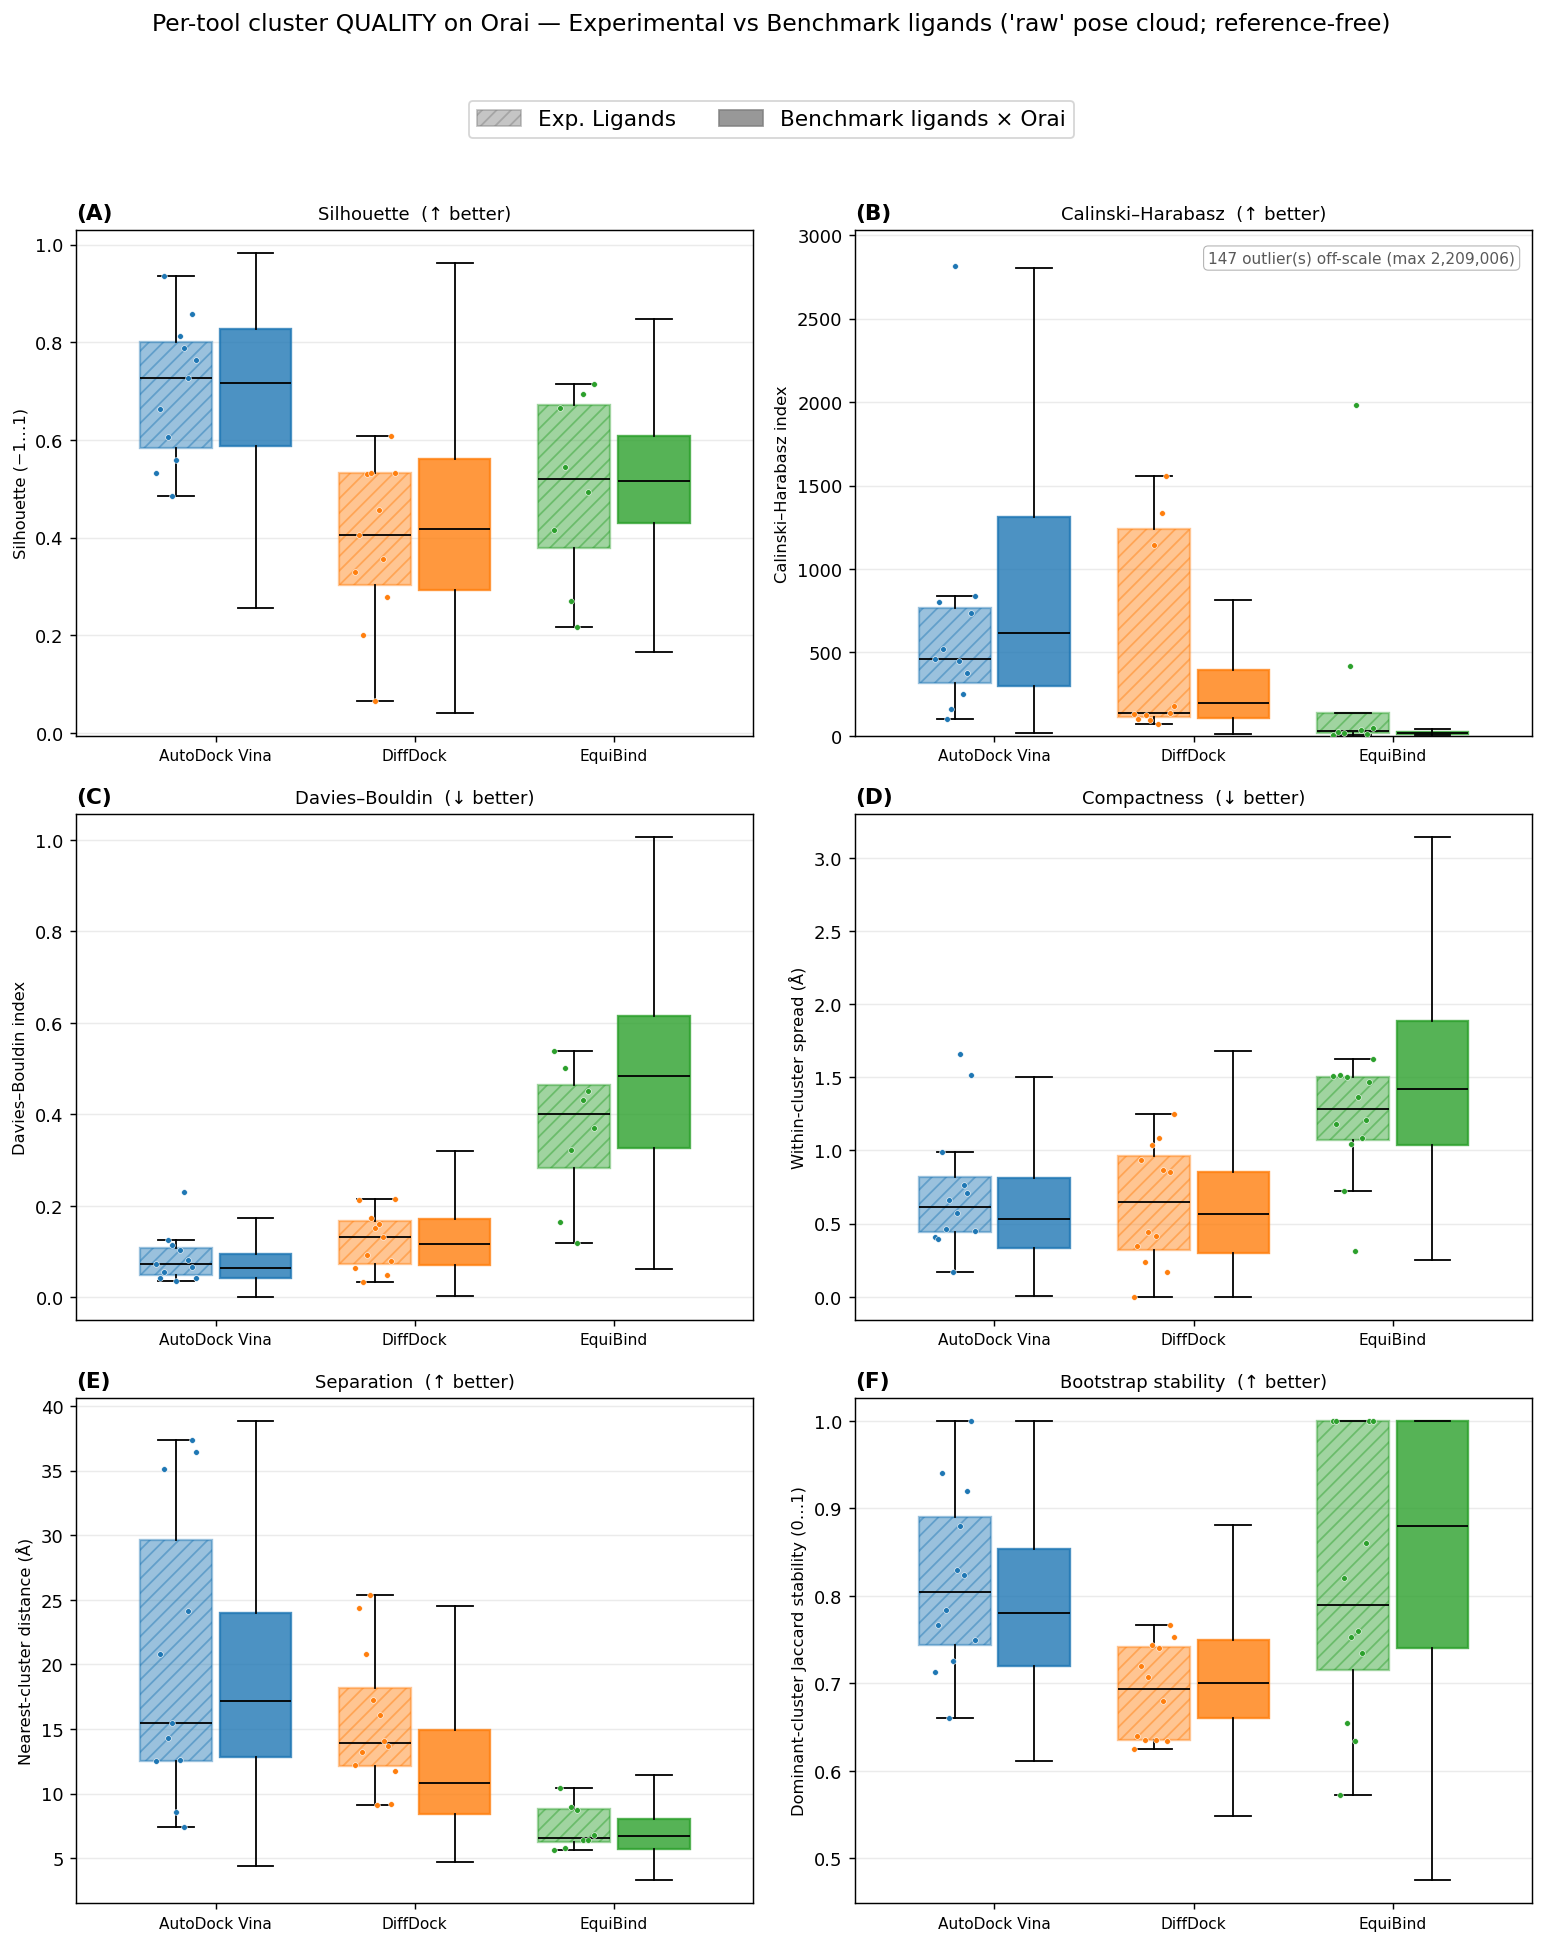
\includegraphics[width=\linewidth,height=0.78\textheight,keepaspectratio]{media/media/image18.png}
\caption[Reference-free cluster quality per tool on Orai]{Reference-free cluster quality per tool on Orai, the experimental ligands against the benchmark control panel on the raw pose cloud. Panel (A) silhouette, panel (B) Calinski-Harabasz index, panel (C) Davies-Bouldin index, panel (D) compactness, panel (E) separation and panel (F) bootstrap stability. Panel (B) is truncated on the vertical axis, with 163 outliers off-scale up to a maximum of 2,209,006}\label{fig:results-r17}
\end{figure}

Figure~\ref{fig:results-r17} reports reference-free cluster quality. AutoDock Vina forms the best-separated clouds in both panels and the most compact benchmark clouds. Experimentally, DiffDock is tighter, with a median within-cluster spread of 0.34\angstrom{} versus 0.62\angstrom{} for AutoDock Vina. EquiBind forms the loosest clouds and often one diffuse mode. High bootstrap stability then indicates reproducibility, not accurate site resolution. Among eighteen tool-by-metric cells, the largest cross-panel gap is DiffDock\textquotesingle s silhouette, with medians of 0.17 experimentally and 0.42 on the benchmark (benchmark-higher \ensuremath{\delta} = +0.53). It reaches Holm p = 0.031 at the frame-ligand unit but 0.548 after each ligand is collapsed across four frames and is therefore descriptive. DiffDock\textquotesingle s Calinski-Harabasz result reverses under that collapse. The sensitivity analysis identifies removal of within-ligand spread rather than new evidence. No other difference was detected. With only three experimental ligands, null results neither establish equivalence nor validate the control panel as a substitute.

\begin{figure}[!htbp]
\centering

\includegraphics[width=\linewidth,height=0.78\textheight,keepaspectratio]{media/media/image19.png}
\caption[Effect of validity and placement filtering on cluster quality]{Effect of validity and placement filtering on cluster quality for the benchmark ligands. Each panel contrasts the raw pose cloud with the filtered cloud of PoseBusters-valid poses outside the transmembrane exclusion slab, for panel (A) within-cluster spread, panel (B) silhouette and panel (C) bootstrap stability. The boxes are the unpaired distributions over every frame-ligand unit that has a cloud of the given kind, whereas the medians and the tests quoted in the text are taken over the units that carry both clouds, so the two readings differ wherever filtering removes most of a tool\textquotesingle s units, most visibly for EquiBind}\label{fig:results-r18}
\end{figure}

Figure~\ref{fig:results-r18} pairs the raw pose cloud against the filtered cloud within each frame-ligand unit of the benchmark panel, across the three quality axes. The medians quoted here are those of the paired subset, that is the units that carry both clouds. For AutoDock Vina and DiffDock it is close to the full panel, but for EquiBind only 64 units on spread and 46 on stability out of 1,232. The EquiBind values therefore sit below the wider raw boxes drawn in the figure. Compactness is essentially unmoved for every tool, AutoDock going from a median 0.52 to 0.50\angstrom{} at a rank-biserial of \ensuremath{-}0.01 (Holm-corrected p = 1.000), DiffDock from 0.57 to 0.57 (p = 1.000) and EquiBind from 1.50 to 1.30 (p = 1.000). Bootstrap stability rises significantly for all three, AutoDock holding a median 0.78 at a rank-biserial of +0.27, DiffDock from 0.70 to 0.72 at +0.54 and EquiBind from 0.95 to 1.00 at +0.99, each with a corrected p below 1e-3. DiffDock also gains on silhouette, from 0.43 to 0.47 at +0.30 and p below 1e-4. The EquiBind rise is degenerate rather than informative, since 39 of its 46 paired filtered clouds collapse to a single cluster. In that case the bootstrap Jaccard stability is identically 1.00 by construction. On the seven paired units that keep more than one cluster the medians move only from 0.67 to 0.74.

\begin{figure}[!htbp]
\centering

\includegraphics[width=\linewidth,height=0.78\textheight,keepaspectratio]{media/media/image20.png}
\caption[Total contacts per pose on Orai]{Total protein-ligand contacts per pose on Orai}\label{fig:results-r19}
\end{figure}

Figure~\ref{fig:results-r19} compares total protein-ligand contacts per pose between the two ligand sets, with the pose-level median printed on each box. The four effect sizes behind the Results reading are the following. At the frame-ligand unit AutoDock gives Cliff\textquotesingle s \ensuremath{\delta} = \ensuremath{-}0.26 on per-complex-mean medians of 26.3 for the benchmark against 30.5 for the experimental set, and DiffDock gives \ensuremath{\delta} = \ensuremath{-}0.27 on 15.7 against 18.2, each at a Holm-adjusted p = 0.205. At the ligand unit AutoDock strengthens to \ensuremath{\delta} = \ensuremath{-}0.33 while DiffDock weakens to \ensuremath{-}0.19, each at a Holm-adjusted p = 0.644.

\begin{longtable}[]{@{}
  >{\raggedright\arraybackslash}p{(\columnwidth - 10\tabcolsep) * \real{0.2600}}
  >{\raggedleft\arraybackslash}p{(\columnwidth - 10\tabcolsep) * \real{0.1500}}
  >{\raggedleft\arraybackslash}p{(\columnwidth - 10\tabcolsep) * \real{0.1500}}
  >{\raggedleft\arraybackslash}p{(\columnwidth - 10\tabcolsep) * \real{0.1300}}
  >{\raggedleft\arraybackslash}p{(\columnwidth - 10\tabcolsep) * \real{0.1550}}
  >{\raggedleft\arraybackslash}p{(\columnwidth - 10\tabcolsep) * \real{0.1550}}@{}}
\caption[Interaction-Type Mean Counts per Pose on Orai1]{Interaction-Type Mean Counts per Pose on Orai1, Benchmark against Experimental Ligands. AD denotes AutoDock Vina and DD DiffDock, each in its selected variant}\label{tab:appendix-orai-interaction}\tabularnewline
\toprule\noalign{}
{\raggedright \textbf{Interaction type}} & \centering\arraybackslash\textbf{AD bench.} & \centering\arraybackslash\textbf{AD exp.} & \centering\arraybackslash\textbf{AD \ensuremath{\delta}} & \centering\arraybackslash\textbf{DD bench.} & \centering\arraybackslash\textbf{DD exp.} \\
\midrule\noalign{}
\endfirsthead
\caption[]{Interaction-Type Mean Counts per Pose on Orai1 (continued)}\tabularnewline
\toprule\noalign{}
{\raggedright \textbf{Interaction type}} & \centering\arraybackslash\textbf{AD bench.} & \centering\arraybackslash\textbf{AD exp.} & \centering\arraybackslash\textbf{AD \ensuremath{\delta}} & \centering\arraybackslash\textbf{DD bench.} & \centering\arraybackslash\textbf{DD exp.} \\
\midrule\noalign{}
\endhead
\bottomrule\noalign{}
\endlastfoot
Hydrogen bond & 4.15 & 2.53 & +0.45 & 2.47 & 1.31 \\
Halogen bond & 0.19 & 1.26 & \ensuremath{-}0.52 & 0.16 & 1.17 \\
Hydrophobic & 3.75 & 5.95 & \ensuremath{-}0.59 & 2.36 & 3.42 \\
Alkyl-\ensuremath{\pi} & 4.90 & 6.67 & \ensuremath{-}0.42 & 3.31 & 5.06 \\
Carbon-\ensuremath{\pi} & 2.55 & 3.55 & \ensuremath{-}0.50 & 1.40 & 1.47 \\
\ensuremath{\pi}-\ensuremath{\pi} stacking & 2.39 & 3.17 & \ensuremath{-}0.41 & 1.29 & 1.19 \\
Amide-\ensuremath{\pi} & 0.92 & 0.95 & \ensuremath{-}0.04 & 0.56 & 0.89 \\
Charged classes & 0.47 & 0.00 & +0.38 & 0.22 & 0.00 \\
Repulsion & 0.43 & 0.00 & +0.31 & 0.37 & 0.00 \\
\multicolumn{6}{@{}p{\dimexpr\columnwidth-6\tabcolsep\relax}@{}}{\footnotesize%
Entries are per-complex mean counts per pose, which is the inferential unit, whereas Figure~\ref{fig:results-r20} plots pose-level means. AD is AutoDock Vina + gnina and DD is DiffDock + smina. Cliff\textquotesingle s \ensuremath{\delta} is oriented so that a positive value means the benchmark ligands are higher. The DiffDock effect sizes run in the same direction as the AutoDock ones on every row except \ensuremath{\pi}-\ensuremath{\pi} stacking, where a DiffDock +0.07 that does not clear correction opposes an AutoDock \ensuremath{-}0.41. The charged classes are reported as a single row because the profiler writes every charged contact three times, once as an ionic contact, once as a salt bridge and once as an attractive-charge contact, so the entry is the value of one of those identical classes and not their sum. EquiBind retains a single usable experimental pose and is therefore omitted. At the frame-ligand unit fourteen of the twenty-six distinct tool-by-type cells clear Benjamini-Hochberg correction, and every one of them appears above. Five rows clear for both tools. The amide-\ensuremath{\pi} row is carried on DiffDock\textquotesingle s account alone and the carbon-\ensuremath{\pi}, \ensuremath{\pi}-\ensuremath{\pi} stacking and charged-classes rows on AutoDock\textquotesingle s. At the ligand unit not one cell does, the smallest adjusted values being 0.089 for AutoDock and 0.106 for DiffDock, so every row is descriptive.} \\
\end{longtable}

\begin{figure}[!htbp]
\centering

\includegraphics[width=\linewidth,height=0.89\textheight,keepaspectratio]{media/media/image22.png}
\caption[Orai residue hot-spots]{Orai residue hot-spots. Percentage of a tool\textquotesingle s poses contacting each of the fifteen most frequently contacted Orai1 residues, with panel (a) AutoDock Vina, panel (b) DiffDock and panel (c) EquiBind. Solid bars are the benchmark ligands and hatched bars the experimental ones. The fifteen are ranked by pooled contact frequency over all 7,458 poses of the six tool-by-ligand-set groups, so each group contributes in proportion to the number of poses it holds and the axis runs from Asp110 at 28.8\% of poses down to Pro146 at 14.7\%}\label{fig:results-r21}
\end{figure}

Figure~\ref{fig:results-r21} reports the percentage of a tool\textquotesingle s poses that touch each of the fifteen most frequently contacted Orai residues. Residues are ranked by pooled contact frequency across the six tool-by-ligand-set groups and weighted by pose count, so no residue reaches the axis on the strength of a group holding very few poses. The per-residue values behind the Results reading are the following. Under AutoDock the modulators sit higher on five of the fifteen frequent residues and lower on ten, the largest raw gap being Ala177 at 40.6\% of poses against 20.4\% of benchmark poses, which alone reaches an uncorrected p below 0.05. DiffDock runs the other way on several residues, engaging Asp110 in 32.1\% of benchmark poses against 11.1\% of modulator poses and Leu109 in 24.4\% against 5.6\%, and its modulator poses essentially abandon Ala177. These pose-level two-proportion tests are both pseudoreplicated and underpowered, and none survives Holm correction. They are descriptive support for the figure rather than inference.

\hypertarget{posebusters-validity-checks}{%
\section{PoseBusters Validity Checks}\label{posebusters-validity-checks}}

Table~\ref{tab:appendix-posebusters-checks} lists the individual checks of the PoseBusters validity battery referenced in the Methods (Physical and Chemical Validity) \cite{ref035}. Twenty-two of the twenty-six listed entries were applied in this work. The four remaining entries compare the docked pose against the co-crystallised reference ligand. None ran in any dataset reported here, because every pose was screened without a reference molecule supplied. PoseBusters defines a fifth reference-based check that this table does not list, namely the RMSD threshold test named in the Methods. It is kept off the validity axis here because near-nativeness is gated separately. That test loads every deposited instance of the ligand and reports the lowest RMSD, which is the copy rule the Methods adopt. The columns of those four entries are consequently absent from the results tables, and a pose is PB-valid only if it passes every applied check. The verdict set also covers two entries that a bare listing of the geometric tests omits. Those two are that the receptor file itself loads and that the ligand has not been placed beyond the maximum permitted distance from the protein.

On the calibration benchmark each pose was screened against the receptor its own docking stage used rather than against one shared file. For AutoDock Vina that is the cleaned PDB that is heavy-atom identical to the PDBQT the search read, and the runner aborts before screening if the two differ. The Orai panels do not inherit that guarantee. They ran under the shared-receptor policy. Every pose was therefore screened against a single file per frame and tool, and the exactness check never applied. On the START-Fr0 frame that file was the delivered structure rather than the energy-minimised one that the AutoDock search alone read (Appendix~\ref{orai1-receptor-model}). Against the delivered structure, 893 of the 3,079 Fr0 AutoDock poses of the control panel failed the minimum-distance check. Rescreening them against their own search receptor left three, and the reported verdicts are those of the rescreen. DiffDock was screened against its own prepared protein file, which carries protein atom records alone, and EquiBind against its prepared receptor, which retains heteroatom records and all-atom hydrogens. Those differences do not carry into the verdicts. The battery ignores hydrogens on every intermolecular check, and the heavy-atom coordinate sets of the AutoDock and DiffDock receptors are identical on 301 of the 303 screened complexes with no AutoDock-only atom anywhere in the remainder. On that identical-receptor subset the minimum-distance-to-protein failure rate is 0.2\% for AutoDock Vina against 32.7\% for DiffDock. The AutoDock figure pools its raw search with its rescored arm over roughly 18,000 poses, and the DiffDock figure pools its raw arm with its two optimised arms over roughly 27,000 poses and is carried by its raw arm at 73.7\%. The selected variants give 0.2\% for AutoDock Vina + gnina against 13.5\% for DiffDock + smina on the same identical-receptor subset. The minimum-distance column of Table~\ref{tab:appendix-pb-decomposition-full}, which is taken over all 303 complexes, gives 0.2 and 13.4\% for the same two variants. The gap holds on either basis, so the spread reported in the Results is a property of the poses rather than of the receptor preparation.

\begin{longtable}[]{@{}
  >{\raggedright\arraybackslash}p{(\columnwidth - 2\tabcolsep) * \real{0.3579}}
  >{\raggedright\arraybackslash}p{(\columnwidth - 2\tabcolsep) * \real{0.6421}}@{}}
\caption[PoseBusters Validity Checks]{PoseBusters Validity Checks}\label{tab:appendix-posebusters-checks}\tabularnewline
\toprule\noalign{}
{\raggedright \textbf{Check}} & {\raggedright \textbf{Description}} \\
\midrule\noalign{}
\endfirsthead
\caption[]{PoseBusters Validity Checks (continued)}\tabularnewline
\toprule\noalign{}
{\raggedright \textbf{Check}} & {\raggedright \textbf{Description}} \\
\midrule\noalign{}
\endhead
\bottomrule\noalign{}
\endlastfoot
\multicolumn{2}{@{}l@{}}{%
\textbf{Chemical validity and consistency}} \\
File loads & The docked pose can be parsed into an RDKit molecule object. \\
Receptor file loads & The receptor structure, together with any retained cofactors, can be parsed so that the intermolecular tests have something to test against. \\
Sanitisation & The molecule passes RDKit's chemical sanitisation checks. \\
InChI convertible & The molecule can be converted to a standard InChI string. \\
All atoms connected & All atoms form a single connected component (no disconnected fragments). \\
No radicals & The molecule contains no unpaired electrons (radical atoms). \\
Molecular formula\footnote{This entry and the three that follow it (bonds, tetrahedral chirality and double-bond stereochemistry) are the reference-based members of the battery. Each needs the co-crystallised ligand as a second input, which was supplied in none of the runs reported here, so all four were not applicable and were not run, and they contribute no columns to the results tables.} & The molecular formula is identical to that of the reference ligand. Not applicable in this work and not run. \\
Bonds & The bond graph (atom connectivity) is identical to the reference ligand. Not applicable in this work and not run. \\
Tetrahedral chirality & Tetrahedral stereocentres match the reference configuration. Not applicable in this work and not run. \\
Double-bond stereochemistry & Double-bond (cis/trans) configuration matches the reference. Not applicable in this work and not run. \\
\multicolumn{2}{@{}l@{}}{%
\textbf{Intramolecular validity (ligand geometry and strain)}} \\
Bond lengths & Every bond length lies within 0.75--1.25 of the RDKit distance-geometry bounds (25\% tolerance). \\
Bond angles & Every bond angle lies within 0.75--1.25 of the distance-geometry bounds. \\
Planar aromatic rings & All atoms of 5- and 6-membered aromatic rings lie within 0.25\angstrom{} of their mean plane. \\
Non-aromatic ring non-flatness & Non-aromatic 6-membered rings deviate from their mean plane by at least 0.05\angstrom{} (they are not spuriously flattened). \\
Planar double bonds & The two carbons of aliphatic C=C bonds and their four substituents lie within 0.25\angstrom{} of their mean plane. \\
Internal steric clash & Non-covalently bound atom pairs are no closer than 0.7 of the distance-geometry lower bound, the value implied by the clash tolerance of 0.3 set in the docking configuration used throughout this work. \\
Internal energy ratio & The UFF energy of the pose is at most 100\ensuremath{\times} the mean energy of a 50-conformer ETKDG ensemble (no gross strain). \\
\multicolumn{2}{@{}l@{}}{%
\textbf{Intermolecular validity (ligand versus receptor)}} \\
Protein--ligand maximum distance & The ligand lies within the maximum permitted separation from the receptor, so it has not been placed away from the protein altogether. \\
Minimum protein--ligand distance & Protein--ligand atom pairs are farther apart than 0.75\ensuremath{\times} the sum of their van der Waals radii. \\
Minimum distance to organic cofactors & Ligand--organic-cofactor atom pairs exceed 0.75\ensuremath{\times} the sum of their van der Waals radii. \\
Minimum distance to inorganic cofactors & Ligand--inorganic-cofactor atom pairs exceed 0.75\ensuremath{\times} the sum of their covalent radii. \\
Minimum distance to waters\footnote{The two water-related checks (minimum distance to waters and volume overlap with waters) were run together with the rest of the battery and are among the twenty-two applied entries, so both contribute verdict columns to the results tables. Receptor preparation left no crystallographic water molecules in any receptor file, so nothing the two checks were designed to catch can be present. The residual failures they report over the eight variants of the decomposition, namely 1,558 poses on minimum distance to waters and 81 on volume overlap with waters, fall entirely on the three EquiBind rows, while the AutoDock Vina and DiffDock rows carry none. Uni-Dock2, a fourth engine screened alongside the others, is omitted from every reported result and from that decomposition. The package attributes these failures to non-water receptor atoms. Every affected pose already fails at least one non-water check, so the set passing all twenty-two applied checks is identical to the set passing the twenty non-water checks and PB-validity is unaffected. The four cofactor checks, namely minimum distance and volume overlap against organic and against inorganic cofactors, need the same audit and it runs the same way. PDBFixer strips cofactors from all but 30 of the AutoDock receptors and DiffDock\textquotesingle s preparation retains none at all, so the four checks record two failures across the AutoDock arms and none across DiffDock. The EquiBind preparation instead retains heteroatom records in 274 of its 308 receptors, so EquiBind alone is systematically screened against cofactors and carries 5,201, 1,223, 1,321 and 339 failures on the four in the order given. Removing all four checks moves 12 of its 80,100 poses across the validity threshold and no pose of any other arm. The asymmetry therefore penalises EquiBind rather than inflating the reported ordering, and PB-validity as used here is a marginally stricter criterion for EquiBind than for the other two arms rather than a weaker one for all three. This is nonetheless a difference from the source benchmark, which ships receptors retaining their cofactors. Section~\ref{autodock-vina-2} reports how much of the benchmark carries a metal at the ligand site and gives the recovery endpoint split by that partition.} & Ligand--water atom pairs exceed 0.75\ensuremath{\times} the sum of their van der Waals radii. \\
Volume overlap with protein & Less than 7.5\% of the ligand volume intersects the protein (van der Waals radii scaled by 0.8). \\
Volume overlap with organic cofactors & Less than 7.5\% of the ligand volume intersects organic cofactors (radii scaled 0.8). \\
Volume overlap with inorganic cofactors & Less than 7.5\% of the ligand volume intersects inorganic cofactors (radii scaled 0.5). \\
Volume overlap with waters & Less than 7.5\% of the ligand volume intersects water molecules (radii scaled 0.5). \\
\end{longtable}

\hypertarget{interaction-fingerprints}{%
\section{Interaction Fingerprints}\label{interaction-fingerprints}}

Only PoseBusters-valid poses are profiled, and on Orai1 only those also lying outside the transmembrane exclusion slab. The retained depth is capped at the top five ranked poses per complex on the calibration benchmark and at the top three ranked poses per frame-ligand unit on Orai1. Every docked pose is then written into a single coordinate file together with its receptor, with the ligand forced to heteroatom records under one reserved residue name. The resulting complex is profiled with PandaMap 4.1.0 \cite{ref090} through its hybrid protein-ligand mapper. Detection is run in the package\textquotesingle s standard mode rather than in its stricter experimental variant, which is not functional in this release, so the classification below is the one actually executed. The profiled pool is the retained valid pose set rather than its near-native subset, being 4,253 poses over 303 complexes with a median deviation of 5.01\angstrom{} from the nearest deposited copy of the crystal ligand and 26.9\% of poses within 2\angstrom{}. Reported overlaps are consequently contact agreement across produced poses and not across correct ones. Two sensitivity analyses measure what that costs, both written by \texttt{interaction\_pose\_basis\_audit.py}. Standardising rank-1 contact recovery to a common placement distribution moves the F1 triple for AutoDock Vina, DiffDock and EquiBind from 0.732, 0.694 and 0.499 to 0.667, 0.647 and 0.628. Roughly four fifths of the separation between the tools is therefore how often each reaches the site rather than which contacts it forms once there, a share running from 82 to 89\% across band schemes of three to fourteen strata. The standardised ordering, AutoDock Vina above DiffDock above EquiBind, holds at every banding, although the spread between the tools shrinks from 0.233 to 0.039. Restricting the fingerprint to poses within 10\angstrom{} of the nearest deposited copy of the crystal ligand, which removes poses placed away from the native site without applying the 2\angstrom{} near-native criterion, raises the mean top-five union overlap to 0.676 over 274 complexes for AutoDock Vina, 0.706 over 262 for DiffDock and 0.623 over 166 for EquiBind, and moves the DiffDock lead over AutoDock Vina from p = 0.011 to p = 2.0e-4 on the shared cohort. That lead holds at every threshold from 8 to 20\angstrom{}. The restriction is conditional rather than corrective. It discards the complexes a tool never reached, namely 27, 38 and 100, and it lifts the share of poses within 2\angstrom{} from 26.9 to 38.8\%.

The contact classes and their thresholds follow the conventions established by PLIP \cite{ref054} and are applied as heavy-atom distance criteria between the ligand and the receptor. A hydrogen bond is recorded between a ligand nitrogen or oxygen and a receptor nitrogen or oxygen separated by 2.4 to 3.5\angstrom{}. A hydrophobic contact is recorded between a ligand carbon and a carbon of alanine, valine, leucine, isoleucine, methionine, phenylalanine, tryptophan, proline or tyrosine within 4.0\angstrom{}. Ionic contacts, salt bridges and attractive-charge contacts between a charged ligand atom and an aspartate or glutamate oxygen or an arginine, lysine or histidine nitrogen use 4.0\angstrom{}. Same-sign repulsion uses 6.0\angstrom{}. The aromatic family, namely pi-stacking, cation-pi, pi-cation, carbon-pi, donor-pi, amide-pi and alkyl-pi, uses 5.5\angstrom{}. Halogen bonds use 3.5\angstrom{} to an oxygen, nitrogen or sulfur acceptor. Metal coordination uses 2.8\angstrom{}, and covalent contacts use 2.1\angstrom{} to the cysteine, serine, lysine or histidine side-chain atoms that can form them. Atom pairs closer than 1.5\angstrom{} are discarded as clashes or coordinate errors. Because angular criteria are not applied in this execution path, a hydrogen bond is a distance-and-atom-type assignment carrying a nominal rather than a measured donor angle, and the aromatic classes are likewise geometric proximity assignments rather than ring-normal tests. Every fingerprint comparison in this work is therefore a comparison of contact patterns under one fixed and uniformly applied definition, not a claim about hydrogen-bond geometry.

Three further defects of this execution path limit what its output can support. The halogen test accepts a ligand atom whose element symbol is written F, Cl, Br or I in mixed case, whereas the structure parser returns element symbols in upper case. Chlorine and bromine can never satisfy it, and only fluorine is ever recorded as a halogen-bond donor in these datasets. All 3,144 halogen-bond records written for the Orai1 control panel are fluorine and not one is chlorine, yet 34 of the 308 calibration ligands carry chlorine and 26 of those carry no fluorine at all. The three experimental modulators are fluorine-only or halogen-free, since 2-APB carries no halogen while Synta-66 carries one fluorine and GSK-7975A five. The blindness therefore suppresses halogen contacts in the control arm and in none of the experimental arm, which inflates the halogen-bond contrast reported in the Results in the same direction that contrast runs. The halogen rows of Table~\ref{tab:appendix-orai-interaction} and Figure~\ref{fig:results-r20} should be read as counts of fluorine-to-acceptor proximity rather than as halogen bonding. The second defect is that a single charged ligand-receptor contact is written out three times, once as an ionic contact, once as a salt bridge and once as an attractive-charge contact, with identical atoms and distance. The charged rows of Table~\ref{tab:appendix-orai-interaction} carry the value of one of those classes rather than their sum, so no count in that table is inflated. The pooled total-contact counts are a different matter, because they sum every class and therefore carry each charged contact three times. That inflation falls on the benchmark arm alone, since the experimental poses form no charged contact at all. It lifts the benchmark mean toward the experimental one, which understates the total-contact difference rather than manufacturing it. The three classes are one measurement and not three independent classes, and the interaction-type family over which the false-discovery-rate correction is applied therefore holds thirteen distinct hypotheses rather than fifteen. The direction of that difference is easy to read backwards, because it is not uniform. Duplicating a low p-value enlarges the family without changing the rank of any hypothesis above it, so those cells become stricter, and only the cells ranked beneath the duplicates become more lenient. The correction reported in the Results is taken over the thirteen. No AutoDock cell changes verdict between the two families. Carbon-\ensuremath{\pi} ranks above the duplicated cells and moves from an adjusted 0.021 as fifteen entries to 0.018 as thirteen, whereas repulsion ranks beneath them and moves from 0.043 to 0.047. Both clear under either count.

The third defect concerns metal coordination, which is emitted without reference to where the ligand sits. The class is written for 6,296 records over 1,662 poses in 121 calibration complexes, and in all 121 every pose carries an identical set of coordinating residues irrespective of its rank or its distance from the crystal ligand. A pose docked elsewhere on the receptor therefore inherits the native metal keys unchanged. Among poses beyond 20\angstrom{} from the nearest deposited copy of the crystal ligand, those carrying no metal contact recover a mean F1 of 0.0012 and only six of 335 recover any native contact at all, whereas those carrying one recover 0.1419 and not one of the 233 scores zero. Nearly all of the residual far-field signal is therefore this artefact. Neither Orai1 panel records a single metal-coordination contact, and the defect touches the calibration benchmark alone. Its effect on the reported similarity is nonetheless small. Removing the class moves the mean top-five union overlap from 0.539, 0.572 and 0.403 to 0.531, 0.564 and 0.389, and repairing both this and the charged duplication leaves 0.532, 0.566 and 0.391. On the shared cohort the Results chapter reports, the DiffDock lead over AutoDock Vina moves from p = 0.011 to 0.013 with the metal class removed and to 0.012 with both repaired. The ordering and its significance are therefore unaffected.

Each detected contact is reduced to a key formed by its interaction class together with the residue name, residue number and chain identifier of the receptor residue involved. The whole-protein preparation used by some engines renumbers residues sequentially from one, and one prepared receptor carries no chain identifiers at all. Left alone, their keys would never match the author-numbered crystal reference and their measured native recovery would collapse towards zero. All poses of the calibration benchmark are therefore profiled against a canonical receptor set that carries author numbering and was verified heavy-atom coordinate-compatible with each tool\textquotesingle s own docking receptor, which relabels residues without moving any atom. The crystal fingerprint is computed for every deposited copy of the ligand on that receptor, and each pose is scored against the copy it lies nearest to, because a pose placed at an alternate copy would otherwise be scored against the residues of a site it does not occupy. A top-five union is scored against the union of the fingerprints of the copies its poses are nearest to. A pose that yields no contact at all is retained with an empty fingerprint and counts as a zero, and a pose whose complex cannot be assembled or parsed is written to a separate error table and excluded from every figure. A mapping failure is therefore never silently scored as an absence of contacts.

EquiBind is ranked by its gnina affinity because it emits no confidence score of its own. Tools are compared on the complexes they share, with a Friedman omnibus across tools followed by Wilcoxon signed-rank pairwise tests under Holm or Benjamini-Hochberg correction. Reporting per pose would treat the several retained poses of one complex as independent observations, which they are not.

\hypertarget{orai1-receptor-model}{%
\chapter{Orai1 Receptor Model}\label{orai1-receptor-model}}

The docking receptor is a homology model built on the sixfold architecture first resolved in the Drosophila melanogaster Orai crystal structure \cite{ref037}. Each of the six identical subunits contributes residues 66 to 288, spanning the tail of the cytoplasmic N-terminus, the four transmembrane helices M1 to M4 and the M4 C-terminal extension. The supplied molecular-dynamics coordinates carry CHARMM hydrogens and CHARMM histidine states. The preparation step removes every hydrogen and renames HSD, HSE and HSP to plain HIS, so the delivered receptor is a purely heavy-atom structure of 10,362 atoms. Polar hydrogens are then re-added by the PDBQT converter under its own geometric and atom-type rules rather than by a titration model. The AutoDock receptor for Fr0 alone took a different path, which the next paragraph sets out.

ADFRsuite \texttt{prepare\_receptor} aborts on the delivered Fr0 coordinates because several covalent bonds in that frame lie beyond the bond-perception cutoff of its hydrogen builder. The first in file order is the bond between C\ensuremath{\alpha} and C\ensuremath{\beta} of Ser93, stretched to 1.85 to 2.06\angstrom{} in every chain, and some chains carry further stretched bonds in Lys203, Leu248, Ile251, Phe253 and His256. The AutoDock preparation fell back to PDBFixer and OpenMM for that frame alone. PDBFixer added the six missing C-terminal OXT atoms and placed hydrogens at a nominal pH of 7.0, and OpenMM then energy-minimised the complete structure in the amber14-all force field with GBn2 implicit solvent. The converter was run on that output. The AutoDock Fr0 search receptor therefore carries the complete 1,338 residues and 10,368 heavy atoms at minimised coordinates, and PoseBusters screened the Fr0 AutoDock poses against those same coordinates. The Fr300, Fr400 and Fr499 search receptors are coordinate-identical to the delivered files, and DiffDock and EquiBind read the delivered heavy-atom coordinates on every frame including Fr0.

The PDBFixer and OpenMM fallback breaks receptor parity on Fr0. The minimised search receptor lies 0.82\angstrom{} from the delivered coordinates over the 10,362 shared heavy atoms and 0.64\angstrom{} over the 1,338 C\ensuremath{\alpha} atoms, with no rigid-body component. The shift exceeds 2\angstrom{} for 149 atoms in 97 residues, 25 of them inside the Arg91 to Glu106 pore slab, and peaks at 3.63\angstrom{} at the side-chain nitrogen of Lys203 in chain A. Among the displaced residues, Tyr80 and Lys87 are the two that occur most often within 4\angstrom{} of a rank-1 Fr0 AutoDock pose. Of the 2,268 polar hydrogens in that file, 2,208 were placed by PDBFixer and the converter added only the second imidazole hydrogen on each of the 60 histidines. The histidine, aspartate, glutamate, lysine and arginine typing matches the other frames, while Fr0 alone carries 18 cysteine thiol hydrogens and six carboxylate termini. The Fr0 cross-tool comparison is consequently not receptor-matched, and the difference is visible at the contact level. Of the 3,079 control-panel Fr0 AutoDock poses, 99.3\% touch a receptor atom within 4\angstrom{} that moved by more than 1\angstrom{}, which is the displacement behind the spurious minimum-distance failures recorded in Appendix~\ref{posebusters-validity-checks}. The shift is nonetheless in place and about a tenth of the 5.88 to 6.02\angstrom{} that separate Fr0 from the later frames after superposition. The within-frame coordinate system the site metrics rely on is therefore unchanged.

The pore-lining signature residues R91, V102 and E106 are quoted in the human Orai1 numbering carried by the supplied model itself, which is offset from the Drosophila crystal numbering and is therefore not taken from that structure. R91 is the basic cytoplasmic residue associated with the R91W severe combined immunodeficiency phenotype, V102 is the hydrophobic gate and E106 forms the selectivity filter.

\begin{figure}[!htbp]
\centering

\includegraphics[width=\linewidth,height=0.78\textheight,keepaspectratio]{media/media/image12.png}
\caption[The docking receptor]{The docking receptor. Cartoon representation of the Fr300 molecular-dynamics snapshot (Orai1WT-MDSnap-Fr300), drawn in an oblique view. The image is a one-off illustrative render prepared in PyMOL for this figure and is not the output of any analysis script, so it carries no measurement and none of the quantities in the surrounding text is read from it}\label{fig:results-r10}
\end{figure}

Figure~\ref{fig:results-r10} shows the Fr300 snapshot, the receptor used throughout the Orai1 results chapter. The view is oblique and the six subunits are not colour-coded, so the hexameric arrangement around the central conduction pore is a property of the model described above rather than something the render itself resolves.

The provenance of the model stops at the coordinates, and the gap is stated here rather than left silent. The files carry membrane-simulation features, namely a periodic box and CHARMM-style residue and atom naming, which together indicate that the frames were drawn from a membrane-embedded simulation. Nothing further was supplied. There is no record of the modelling program or the template Protein Data Bank identifiers used to build the homology model, of the force field name or version, of the lipid composition of the bilayer, of the solvent and ion treatment, of the trajectory length, of the identity of the replicate or of the simulation times of the four frames. No part of that metadata is reconstructed or inferred here. Every statement in this work that depends on the receptor therefore rests on the coordinates as delivered, the AutoDock copy of Fr0 excepted, and the four frames are treated as four unlabelled conformational samples of one membrane simulation rather than as timed points along a characterised trajectory.

The four frames also occupy separate molecular-dynamics coordinate systems. Raw C\ensuremath{\alpha} displacement before receptor superposition therefore mixes conformational change with rigid-body translation and rotation, and is not interpreted as structural spread. The aligned comparison behind the frame-spread statement of the Results chapter was carried out for that reason. The cross-frame pose analysis itself continues to use alignment-free residue-contact fingerprints folded onto residue number across the symmetric hexamer.

\hypertarget{choice-of-the-four-receptor-states}{%
\section{Choice of the Four Receptor States}\label{choice-of-the-four-receptor-states}}

All three pipelines treat the receptor as rigid. AutoDock Vina samples ligand torsions against a fixed precomputed grid, and DiffDock and EquiBind condition on a fixed receptor graph. Receptor flexibility can therefore be represented only implicitly, by docking against more than one receptor conformation. Carrying four states rather than one is the standard and computationally inexpensive way to do that.

Orai1 is a poor candidate for single-structure docking on structural grounds. Pore opening proceeds through a widening of the interfaces that the transmembrane helix M3 forms with the non-pore-lining helices \cite{ref072}, which is the lipid-facing interfacial region where small-molecule Orai modulators are proposed to bind. The second candidate region is the calcium-accumulating region, an extracellular loop near the selectivity filter that raises the local calcium concentration at the outer channel mouth and carries the aspartates Asp110, Asp112 and Asp114 \cite{ref038}. Loop conformations are the least well determined part of any homology-derived model and fluctuate in simulation. A single static conformer would over-weight one arbitrary geometry of exactly the two regions the Orai1 chapter asks about.

The spread the four states actually span was measured for this appendix rather than assumed. After rigid superposition on all 1,338 C\ensuremath{\alpha} atoms, the three later frames lie 0.93 to 1.19\angstrom{} from one another, whereas the delivered Fr0 lies 5.88 to 6.02\angstrom{} from each of them and its minimised AutoDock copy 5.84 to 5.98\angstrom{}. Fr0 is thus not a member of the ensemble the later frames sample, which is consistent with its role as the starting structure and with the separate \texttt{START} label its coordinate file carries. Table~\ref{tab:appendix-frame-geometry} resolves where that difference sits, reporting the mean distance of a diagnostic atom from the pore axis over the six subunits, with the axis taken as the principal axis of the C\ensuremath{\alpha} coordinates.

\begingroup
\scriptsize
\begin{longtable}[]{@{}lrrrr@{}}
\caption[Receptor Geometry Across the Four Frames]{Receptor Geometry Across the Four Frames. Mean distance from the pore axis in \angstrom{}, averaged over the six subunits}\label{tab:appendix-frame-geometry}\tabularnewline
\toprule\noalign{}
\textbf{Diagnostic atom} & \textbf{Fr0} & \textbf{Fr300} & \textbf{Fr400} & \textbf{Fr499} \\
\midrule\noalign{}
\endfirsthead
\toprule\noalign{}
\textbf{Diagnostic atom} & \textbf{Fr0} & \textbf{Fr300} & \textbf{Fr400} & \textbf{Fr499} \\
\midrule\noalign{}
\endhead
\bottomrule\noalign{}
\endlastfoot
Arg91 CZ, cytosolic gate & 4.48 & 4.82 & 4.86 & 4.72 \\
Glu106 CD, selectivity filter & 5.01 & 5.83 & 5.75 & 5.76 \\
Asp110 CG, accumulating region & 6.99 & 10.50 & 11.02 & 10.95 \\
Asp112 CG, accumulating region & 8.92 & 14.08 & 14.21 & 14.19 \\
Asp114 CG, accumulating region & 16.34 & 19.26 & 19.97 & 20.22 \\
\end{longtable}
\endgroup

Two things follow. First, the conduction pathway itself is nearly invariant across the three later frames, at 0.14\angstrom{} of spread at the Arg91 gate and 0.08\angstrom{} at the Glu106 filter. The simulation does not open the pore, and the ensemble describes a resting channel throughout. Second, the variation that does exist sits in the extracellular loop, where the spread reaches 0.96\angstrom{} at Asp114, several times the pore figure. The ensemble therefore varies the region the placement hypothesis concerns while holding the pore closed, which is the behaviour the design needs.

Fr0 is kept alongside the later frames for a second reason. DiffDock and EquiBind were trained almost exclusively on crystallographic receptor geometries. Thermally sampled coordinates, with fully resolved side chains and non-idealised loops, are further from that training distribution than an energy-minimised model is, and they are not further from it for a physics-based scoring function. Fr0 against the three later frames is accordingly a contrast between a starting and a thermally sampled receptor geometry, controlled for DiffDock and EquiBind and confounded for AutoDock by the preparation minimisation described above. The measured offsets make the contrast concrete, since Fr0 is 3.5 to 5.2\angstrom{} more compact than the mean of the later frames at the three aspartates while differing by only 0.3 to 0.8\angstrom{} at the gate and the filter. The compaction is confined to the loop rather than distributed over the fold.

Four states are what turn receptor conformation into an explicit factor rather than an uncontrolled nuisance variable, which is what permits the frame-level tests the Results chapter reports. The limits of that are equally explicit. Three later frames sample an equilibrium ensemble sparsely, and the design supports a sensitivity statement rather than a claim of conformational coverage. All four states derive from one simulation of the wild-type channel without STIM1, so nothing here speaks to the STIM1-activated conformation. The frames may also be statistically dependent, and the simulation times that would settle the question are among the metadata the section above records as unavailable. No conformation-selection heuristic was applied by this study, which matters because choosing frames by pocket volume or by docking score would have biased the comparison toward whichever pipeline favours the selected geometry.

Pocket detection identifies the elongated ion pore as the top-ranked cavity in each frame, with M1 residues 66 to 110 and additional transmembrane residues in the more open frame. This region overlaps the functionally implicated pore and filter environment \cite{ref070}, \cite{ref071}, but it is not a conventional buried hydrophobic pocket. The complementary geometric finder returns hundreds of low-druggability cavities, illustrating why blind site selection is unusually difficult on this membrane channel.

\hypertarget{experimental-ligand-pharmacology}{%
\chapter{Experimental Ligand Pharmacology}\label{experimental-ligand-pharmacology}}

The three experimental compounds introduced with the experimental dataset in Section~\ref{experimental-dataset} are described pharmacologically here. Table~\ref{tab:appendix-orai-pharmacology} collects the reported potencies, the assays that produced them and the proposed sites.

\begin{longtable}[]{@{}
  >{\raggedright\arraybackslash}p{(\columnwidth - 6\tabcolsep) * \real{0.2000}}
  >{\raggedright\arraybackslash}p{(\columnwidth - 6\tabcolsep) * \real{0.2700}}
  >{\raggedright\arraybackslash}p{(\columnwidth - 6\tabcolsep) * \real{0.2650}}
  >{\raggedright\arraybackslash}p{(\columnwidth - 6\tabcolsep) * \real{0.2650}}@{}}
\caption[Reported potencies and proposed sites of the experimental Orai1 ligands]{Reported Potencies, Assays and Proposed Sites of the Experimental Orai1 Ligands}\label{tab:appendix-orai-pharmacology}\tabularnewline
\toprule\noalign{}
{\raggedright \textbf{Property}} & \centering\arraybackslash\textbf{2-APB} & \centering\arraybackslash\textbf{GSK-7975A} & \centering\arraybackslash\textbf{Synta-66} \\
\midrule\noalign{}
\endfirsthead
\caption[]{Reported Potencies, Assays and Proposed Sites of the Experimental Orai1 Ligands (continued)}\tabularnewline
\toprule\noalign{}
{\raggedright \textbf{Property}} & \centering\arraybackslash\textbf{2-APB} & \centering\arraybackslash\textbf{GSK-7975A} & \centering\arraybackslash\textbf{Synta-66} \\
\midrule\noalign{}
\endhead
\bottomrule\noalign{}
\endlastfoot
\textbf{Reported \ensuremath{\mathrm{IC}_{50}} (\ensuremath{\mu}M)} & potentiates at 1 to 5, blocks above 10 and robustly at 50 \cite{ref070} & 3.8--4.1 (Orai3, Orai1) \cite{ref070} & 1.0--3.0, no recombinant Orai1 value reported \cite{ref071} \\
\textbf{Assay} & CRAC current \cite{ref070} & whole-cell patch clamp, overexpressed Orai1 and Orai3 \cite{ref070} & native CRAC current, RBL cells \cite{ref071} \\
\textbf{Proposed Site} & not experimentally resolved, functional two-site evidence \cite{ref040} & putative selectivity filter (E106), proposed as allosteric, from mutagenesis and pore-geometry dependence \cite{ref070} & extracellular TM1/TM3 and loops 1/3, from docking, molecular dynamics and mutagenesis \cite{ref071} \\
\multicolumn{4}{@{}p{\dimexpr\columnwidth-4\tabcolsep\relax}@{}}{\footnotesize%
Derler et al. also report 0.8~\ensuremath{\mu}M for GSK-7975A in RBL cells \cite{ref070}. No single inhibitory \ensuremath{\mathrm{IC}_{50}} is quoted for 2-APB because its action is biphasic and assay-dependent \cite{ref070}. Proposed sites are model-derived and filter-proximal rather than experimentally resolved ligand-bound poses. No cognate Orai1 complex is resolved for any compound.} \\
\end{longtable}

GSK-7975A is a pyrazole-derived Orai blocker and the most selective of the three, though not a clean Orai1 tool in native tissue. Against L-type voltage-gated calcium channels its half-maximal inhibitory concentration is roughly 8 \ensuremath{\mu}M, and TRPV6 is the only other channel the source tested outside the Orai family \cite{ref070}. Its sensitivity is tied to selectivity-filter geometry through an allosteric effect, which the source proposes rather than demonstrates. The pore mutant Orai1-E106D is markedly less sensitive, the outer-pore triple mutant Orai1-D110/112/114A leaves potency intact, and 2-APB-gated Orai3 is similarly resistant \cite{ref070}. That is a mutagenesis-derived link to the filter environment and not a resolved ligand pocket. Extracellular application blocks the current, and the compound does not disturb STIM1 puncta formation or STIM1 to Orai1 coupling \cite{ref070}. It therefore acts on the channel rather than as an upstream inhibitor. The cited evidence does not establish that the extracellular face is its only route of access. Selectivity liabilities are real and not confined to TRPV6, which it blocks at 10 \ensuremath{\mu}M as completely and as rapidly as trivalent lanthanum \cite{ref070}. In mouse aorta its most sensitive action is on non-selective cation channel-mediated contraction rather than on contractile store refilling \cite{ref041}. In a preparation with appreciable non-selective or voltage-gated conductance a GSK-7975A effect is therefore not automatically an Orai1 effect.

Synta-66 is an aryl-amide Orai1 blocker with a markedly different isoform fingerprint. It abolishes Orai1 function while potentiating Orai2 and leaving Orai3 untouched \cite{ref093}. That makes it a probe of Orai1 dependence rather than a general Orai blocker. Waldherr et al. localise its action to an extracellular site formed by the outer parts of TM1 and TM3 together with extracellular loops 1 and 3, immediately adjacent to the selectivity filter. The mapping rests on reduced inhibition in the loop1 mutants L109D, H113G and Y115G and the loop3 mutants F199G, P201G and L202G, together with molecular dynamics showing the compound anchoring progressively deeper towards the filter \cite{ref071}. Additional sites are not excluded, but the peer-reviewed evidence points to the extracellular face rather than to both faces of the hexamer. Consistent with a filter-proximal site, E106D largely abolishes the block, and STIM1 puncta formation and STIM1 to Orai1 coupling are unaffected \cite{ref071}. The block also depends on calcium-selective permeation, since in divalent-free sodium solution 10 \ensuremath{\mu}M inhibits wild-type Orai1 only partially whereas the same protocol in calcium gives complete block \cite{ref071}. Potency should therefore not be quantified under divalent-free conditions or in non-selective mutants.

The docking input 2abp-NH2 is native 2-APB (2-aminoethoxydiphenyl borate) in its neutral protonation state. The pharmacology below therefore describes the docked molecule directly. 2-APB is the oldest and least selective of the three and is a bimodal modulator rather than an inhibitor. On the channel its sign reverses with concentration, overexpressed Orai1 being potentiated at low micromolar and inhibited at high. Orai2 is less sensitive to that inhibition and Orai3 is potentiated even at high concentration \cite{ref070}. On Orai3 it does more than gate the channel. It widens the minimum pore from about 3.8\angstrom{} in the store-operated state to more than 5.34\angstrom{} and destroys calcium selectivity, allowing monovalent ions to permeate in both directions \cite{ref092}. It also acts on the sensor. Wei et al. show that it leaves STIM1 to STIM1 interactions unchanged while enhancing the intramolecular coupling between CC1 and SOAR, locking STIM1 towards its autoinhibited resting state \cite{ref040}. One consequence matters for interpretation. Inhibition of puncta and inhibition of store-operated entry are dissociable, since co-expression of Orai1 abolishes the puncta effect while the entry block persists \cite{ref040}. A 2-APB-sensitive signal therefore identifies neither module.

Read as a set, the three ligands span a micromolar Orai1 and Orai3 pore block, an Orai1-selective extracellular block with an internal Orai2 contrast, and a bimodal modulator that acts both on the pore and on the STIM1 sensor. The evidence for GSK-7975A and Synta-66 converges on the extracellular pore mouth and the selectivity filter, which is what the placement criterion of the Results chapter encodes. For 2-APB, whose site is unresolved and whose STIM1 arm is cytosolic, that criterion is a uniform study assumption rather than an established fact. The biologically defensible region is therefore not identical across the three compounds, and they should not be described as sharing one proven binding site.

The docked structure of 2-APB is the neutral protonation state. Its aminoethyl nitrogen is basic enough that a protonated fraction is expected at physiological pH, which is an inference from the chemistry rather than a measured value taken from a cited source. Poses for the cationic form are not sampled here and remain for separate validation.

\hypertarget{dataset}{%
\chapter{Dataset}\label{dataset}}

Every figure, table and count in this chapter describes the 308 benchmark entries introduced in the Methods, enumerated in \texttt{posebusters\_pdb\_ccd\_ids.txt} and published by the PoseBusters authors through the project repository \cite{ref035}. The copy of the distribution held for this work also ships a larger list of 428 entries in \texttt{posebusters\_benchmark\_set\_ids.txt}, the set as it stood in the earlier preprint release. From that set the benchmark authors withdrew 120 entries whose ligands lie within 5.0\angstrom{} of a protein symmetry mate and therefore carry crystal contacts. The chapter maps the chemical and structural breadth of the source set and compares it with the three Orai1-related docking inputs.

\hypertarget{composition-and-provenance}{%
\section{Composition and Provenance}\label{composition-and-provenance}}

Each of the 308 entries pairs one receptor with one cognate ligand. Every complex carries a distinct PDB identifier and a distinct ligand (308 unique PDB IDs and 308 unique chemical-component codes)\footnote{For every entry the benchmark provides four files, namely the protein structure without the ligand of interest, without solvent and with all cofactors (*\_protein.pdb), all crystallographic instances of the ligand of interest (*\_ligands.sdf), one of those instances, which the benchmark supplies to mark the binding site for docking methods that require one and which is the first record of the multi-instance file (*\_ligand.sdf), and one computer-generated starting conformer produced with RDKit's ETKDGv3 algorithm followed by UFF minimisation (*\_ligand\_start\_conf.sdf).}. The crystallographic pose is the experimentally validated reference for scoring every docked pose, while the generated start conformer mimics the ligand information a docking engine sees at runtime.

The experimentally resolved ligand conformations provide the reference for symmetry-corrected pose comparison. A later PDB release date is nonetheless not proof that the biological or chemical pattern was absent from training data, since homology-, pocket-, scaffold- and template-similarity analyses would be needed before a strong no-leakage claim could be made. In 143 of the 308 entries the deposited file holds more than one copy of the ligand, 138 of them among the 303 analysed complexes, and the nearest other copy lies a median 36.0\angstrom{} from the reference over those 143. Every pose is scored against the nearest deposited copy, and the form, centroid and interaction references follow that copy. The source benchmark scored every method this way. Its 25\angstrom{} cube centred on the reference kept almost every other copy outside Vina\textquotesingle s search, whereas the whole-protein box used here contains every one of them, so the convention is live for all three tools in this study. The choice of copy can lower a form count where the copies differ in conformation, and it does so for one complex in each of five printed variants of Table~\ref{tab:results-pose-production}. Four alternates do not share the reference pocket (7A9E\_R4W, 7TUO\_KL9, 7VKZ\_NOJ, 7Z1Q\_NIO) and no complex gains recovery through any of them.

\hypertarget{ligand-physicochemical-profile}{%
\section{Ligand Physicochemical Profile}\label{ligand-physicochemical-profile}}

The 308 source ligands cover a wide region of chemical space. The median ligand has 24 heavy atoms, with an interquartile range of 16 to 32 and a full range of 6 to 64. The median molecular weight is 359 Da. The distributions are right-skewed and extend beyond 600 Da, reflecting peptides, nucleotides, sugars and cofactor-like molecules alongside conventional small molecules (Figure~\ref{fig:appendix-dataset-1}). Table~\ref{tab:appendix-ligand-distribution} summarises the corresponding descriptors. The median ligand has five rotatable bonds, six hydrogen-bond acceptors, three donors and a topological polar surface area of 107\angstrom{}\textsuperscript{2}.

\begin{figure}[!htbp]
\centering

\includegraphics[width=\linewidth,height=0.78\textheight,keepaspectratio]{media/media/image33.png}
\caption[Univariate descriptor distributions]{Univariate distributions of twelve physicochemical attributes across the 308 benchmark ligands}\label{fig:appendix-dataset-1}
\end{figure}

\begin{longtable}[]{@{}
  >{\raggedright\arraybackslash}p{(\columnwidth - 6\tabcolsep) * \real{0.3528}}
  >{\raggedright\arraybackslash}p{(\columnwidth - 6\tabcolsep) * \real{0.1472}}
  >{\raggedright\arraybackslash}p{(\columnwidth - 6\tabcolsep) * \real{0.2500}}
  >{\raggedright\arraybackslash}p{(\columnwidth - 6\tabcolsep) * \real{0.2500}}@{}}
\caption[Principal Ligand Descriptors of the Benchmark]{Distribution of Principal Ligand Descriptors in the PoseBusters Benchmark}\label{tab:appendix-ligand-distribution}\tabularnewline
\toprule\noalign{}
{\raggedright \textbf{Descriptor}} & {\raggedright \textbf{Median}} & {\raggedright \textbf{IQR (25--75\,\%)}} & {\raggedright \textbf{Range (min--max)}} \\
\midrule\noalign{}
\endfirsthead
\caption[]{Distribution of Principal Ligand Descriptors in the PoseBusters Benchmark (continued)}\tabularnewline
\toprule\noalign{}
{\raggedright \textbf{Descriptor}} & {\raggedright \textbf{Median}} & {\raggedright \textbf{IQR (25--75\,\%)}} & {\raggedright \textbf{Range (min--max)}} \\
\midrule\noalign{}
\endhead
\bottomrule\noalign{}
\endlastfoot
Heavy atoms & 24 & 16--32 & 6--64 \\
Molecular weight (Da) & 359 & 236--462 & 100--872 \\
Rotatable bonds & 5 & 2--7 & 0--20 \\
H-bond acceptors & 6 & 3--9 & 0--21 \\
H-bond donors & 3 & 2--5 & 0--13 \\
TPSA (\angstrom{}\textsuperscript{2}) & 107 & 66--160 & 0--384 \\
cLogP & 0.9 & \ensuremath{-}1.6--3.2 & \ensuremath{-}8.4--14.0 \\
Fraction sp\textsuperscript{3} C & 0.41 & 0.23--0.57 & 0.00--1.00 \\
QED & 0.43 & 0.29--0.60 & 0.04--0.91 \\
Ring count & 3 & 1--4 & 0--8 \\
\end{longtable}

\hypertarget{drug-likeness}{%
\section{Drug-Likeness}\label{drug-likeness}}

Drug-likeness metrics confirm that the set deliberately reaches past classical small-molecule drug space. Under Lipinski's rule of five,\footnote{Lipinski's ``rule of five'' is a heuristic for oral drug-likeness. Poor absorption or permeation is more likely when a compound has more than five hydrogen-bond donors, more than ten hydrogen-bond acceptors, a molecular weight above 500 Da, or a calculated logP (cLogP) above 5, each threshold being a multiple of five. See C. A. Lipinski, F. Lombardo, B. W. Dominy and P. J. Feeney, ``Experimental and computational approaches to estimate solubility and permeability in drug discovery and development settings'', Advanced Drug Delivery Reviews, 1997, 23 (1--3), 3--25 (DOI: 10.1016/S0169-409X(96)00423-1).} 83\% of ligands incur at most one violation and 65\% none at all, yet a substantial 17\% violate two or more criteria (Figure~\ref{fig:appendix-dataset-2}). The quantitative estimate of drug-likeness (QED) sits at a median of just 0.43, and only 67\% of ligands clear the 0.34 threshold usually called ``attractive''. This spread is intentional. Keeping polar, charged and oversized ligands stresses each method's ability to generalise rather than rewarding performance on an easy, lead-like subset.

\begin{figure}[!htbp]
\centering

\includegraphics[width=\linewidth,height=0.78\textheight,keepaspectratio]{media/media/image34.png}
\caption[Drug-likeness of the benchmark ligands]{Drug-likeness of the benchmark ligands. Lipinski rule-of-five violation counts (A), overall rule-of-five compliance (B) and the QED distribution (C)}\label{fig:appendix-dataset-2}
\end{figure}

\hypertarget{elemental-and-charge-composition}{%
\section{Elemental and Charge Composition}\label{elemental-and-charge-composition}}

The elemental make-up widens the challenge further (Figure~\ref{fig:appendix-dataset-3}). Roughly a quarter of the ligands contain phosphorus (25\%) or sulfur (24\%), 22\% carry at least one halogen, and metal atoms are essentially absent from the ligand records. In 143 of the 308 entries, 46\%, the deposited structure holds more than one copy of the ligand of interest, and 138 of those are among the 303 analysed complexes. Net formal charges are uncommon, since only 3\% of ligands are charged and the vast majority are neutral. The heteroatom count is nonetheless high and broadly spread (median 8, reaching nearly 30), matching the many nucleotide- and phosphate-containing species. These are exactly the features that the physical and chemical validity checks, namely protonation, geometry and steric clashes, probe most sharply.

\begin{figure}[!htbp]
\centering
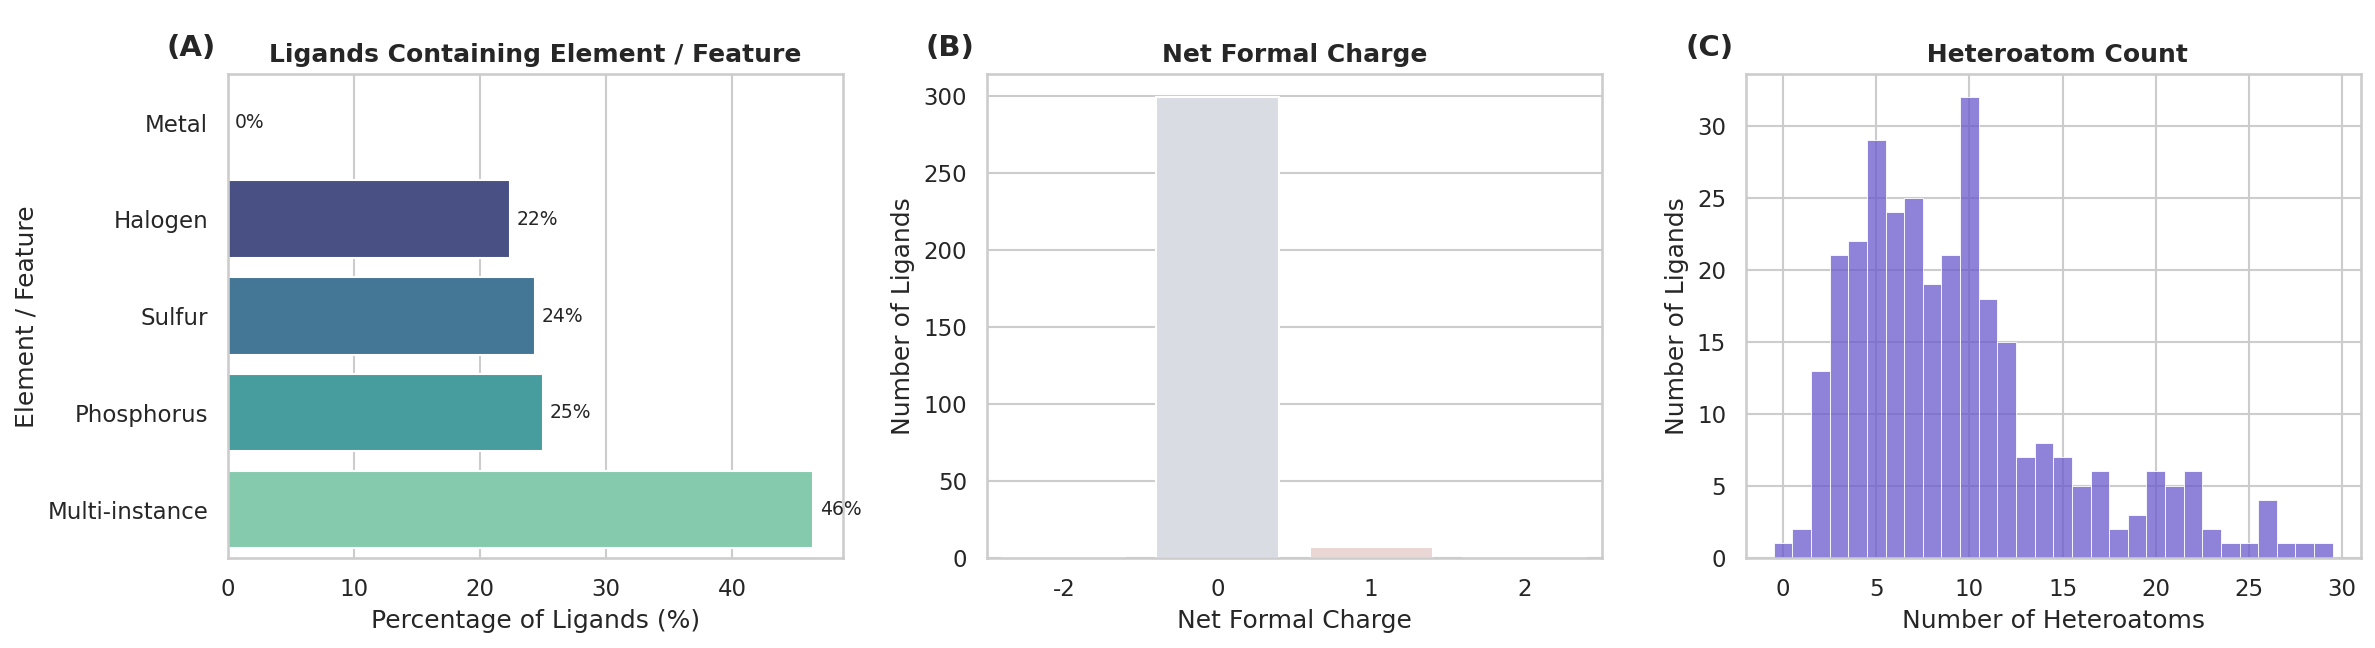
\includegraphics[width=\linewidth,height=0.78\textheight,keepaspectratio]{media/media/image35.png}
\caption[Elemental and charge composition]{Elemental and charge composition. Prevalence of selected elements and features (A), formal-charge distribution (B) and heteroatom counts (C)}\label{fig:appendix-dataset-3}
\end{figure}

\hypertarget{joint-distributions-and-correlation-structure}{%
\section{Joint Distributions and Correlation Structure}\label{joint-distributions-and-correlation-structure}}

The descriptors are considerably interdependent (Figure~\ref{fig:appendix-dataset-4}). The size-related quantities, namely heavy-atom count, molecular weight, hydrogen-bond acceptor count, polar surface area and heteroatom count, correlate strongly and positively. QED falls as molecules grow larger and more polar. Lipophilicity runs opposite to polar surface area, and the sp\textsuperscript{3}-carbon fraction opposes aromatic-ring count, separating flat aromatic scaffolds from saturated three-dimensional ones. The two-dimensional mappings make this explicit. Heavy-atom and rotatable-bond counts rise together (r = +0.70) (Figure~\ref{fig:appendix-dataset-5}\,(A)). Mass and polar surface area co-vary (r = +0.66), lipophilicity and polarity trade off (r = \ensuremath{-}0.61), and drug-likeness declines with size (r = \ensuremath{-}0.52) (Figure~\ref{fig:appendix-dataset-5}). The pairwise joint distributions of the six core descriptors (Figure~\ref{fig:appendix-dataset-6}) confirm that the benchmark forms one broad cloud rather than distinct clusters.

\begin{figure}[!htbp]
\centering
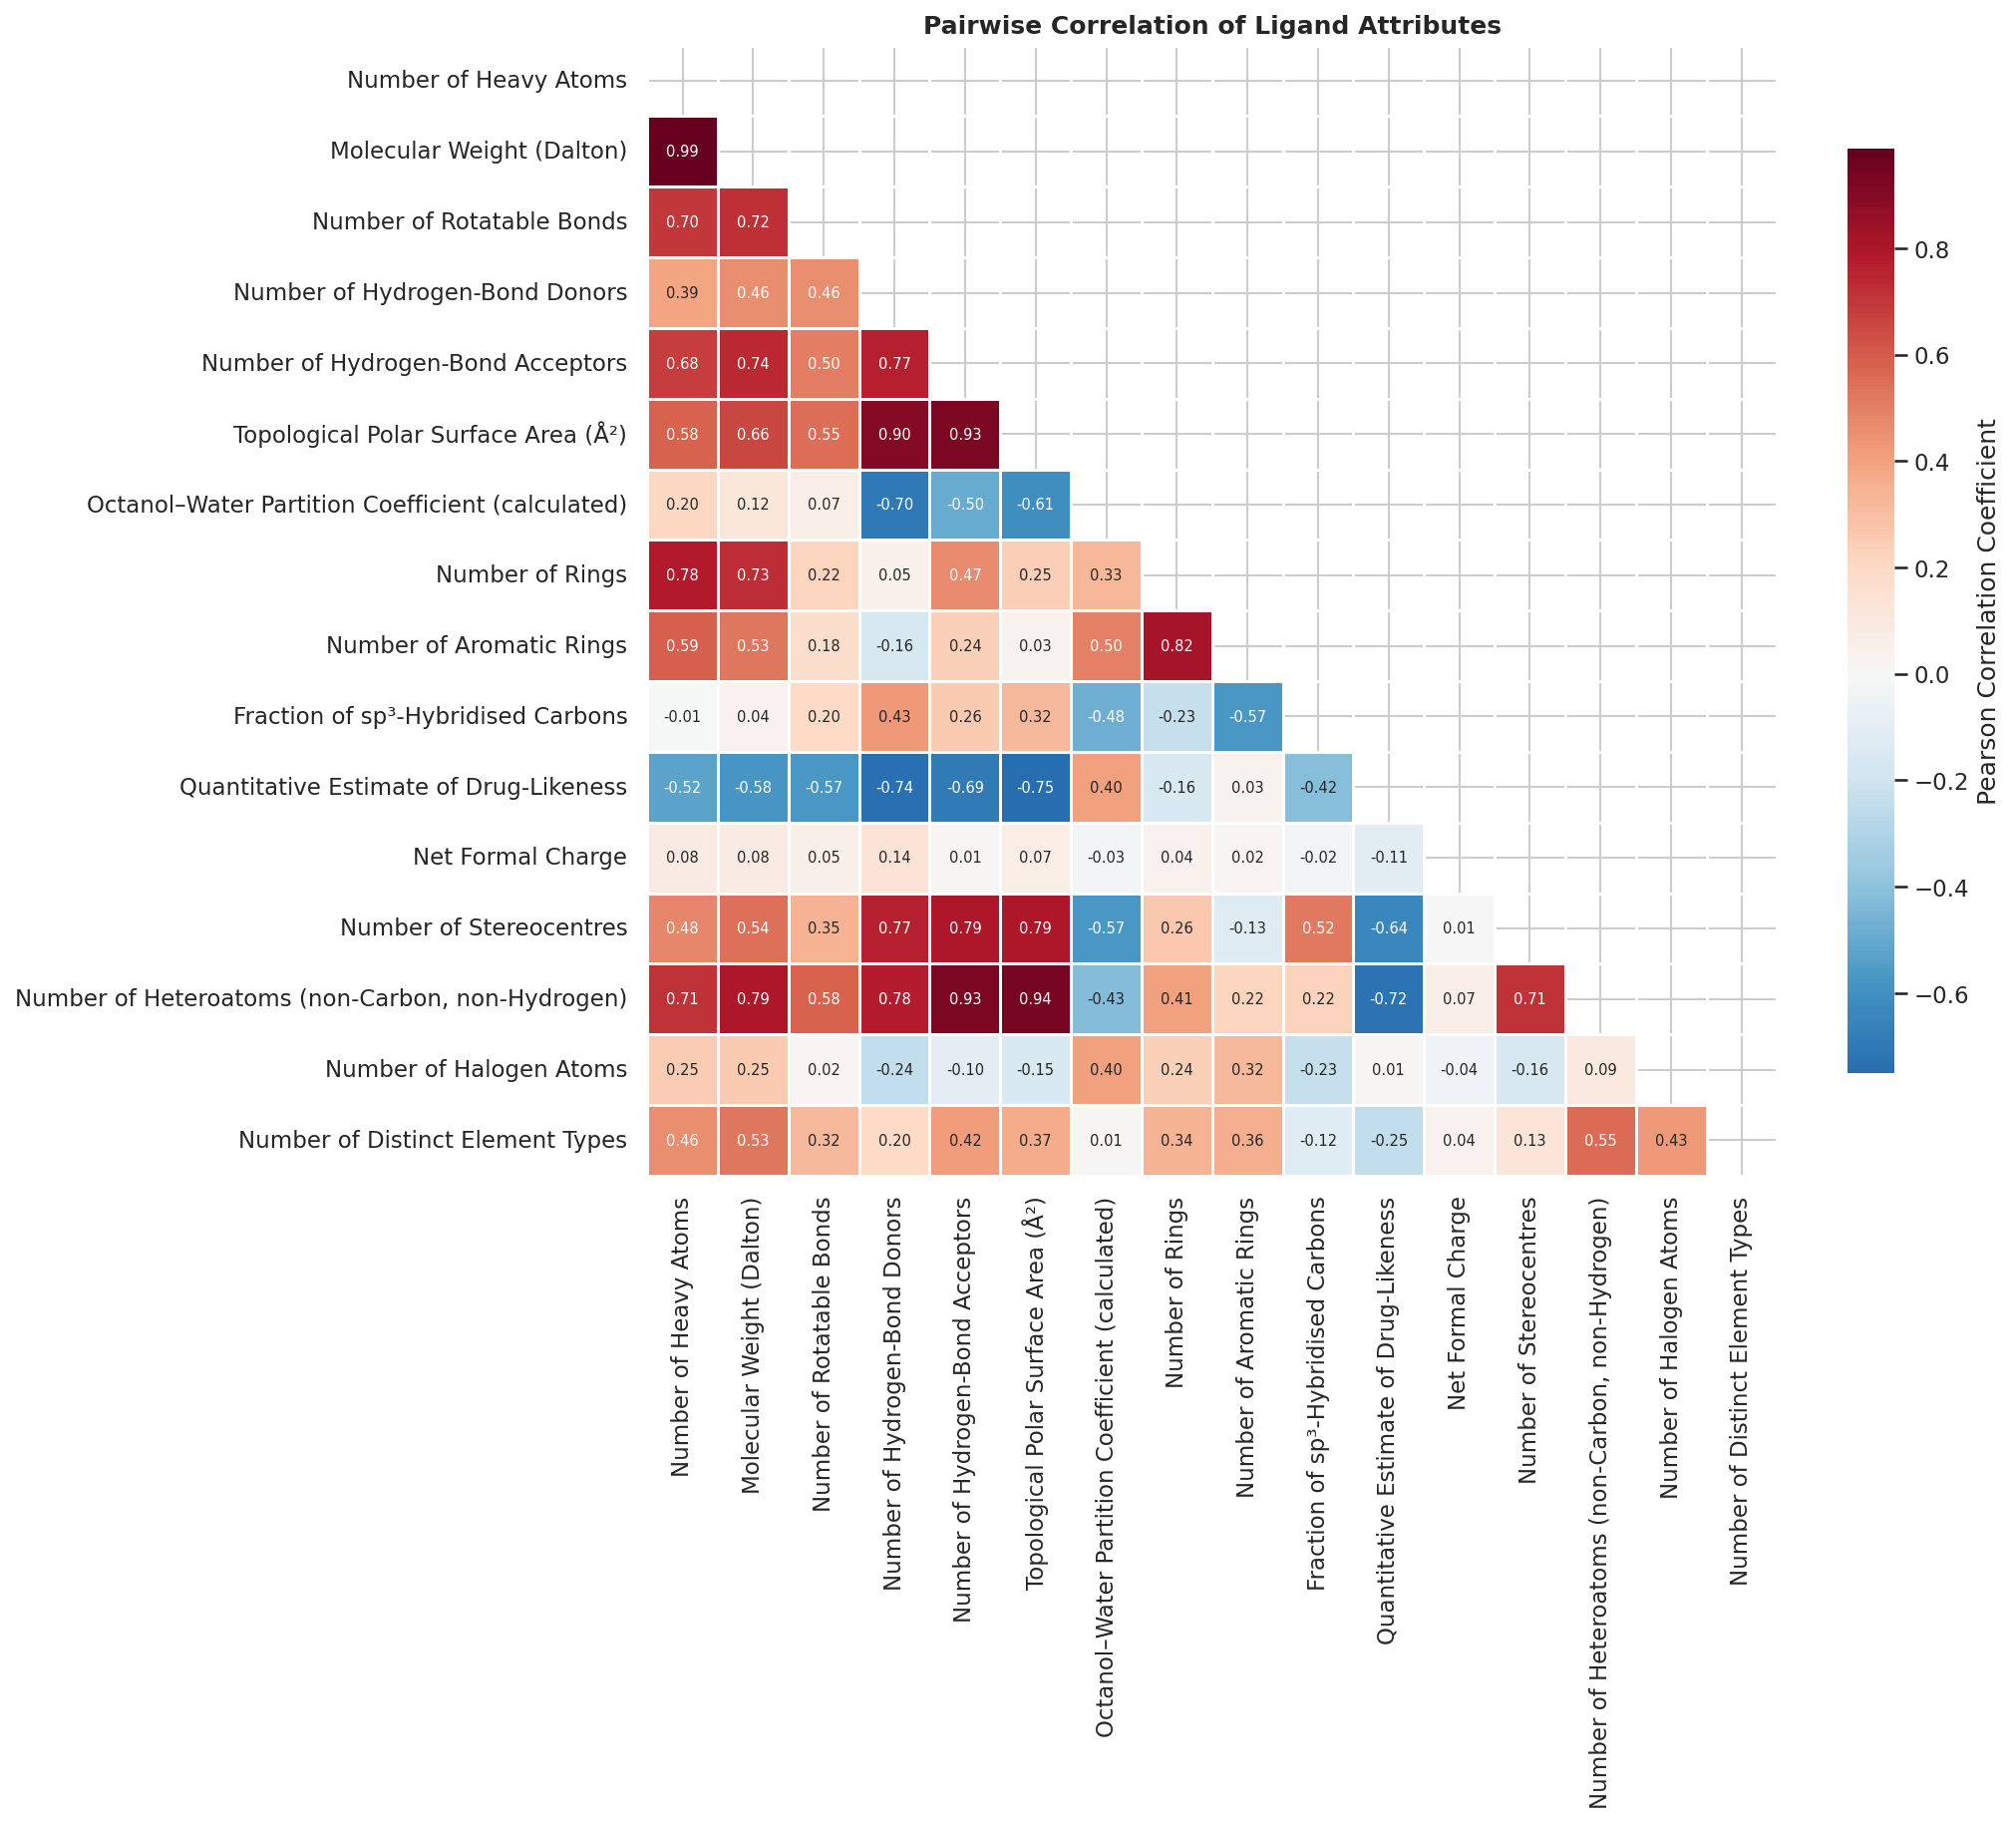
\includegraphics[width=\linewidth,height=0.78\textheight,keepaspectratio]{media/media/image36.png}
\caption[Descriptor correlation matrix]{Pairwise Pearson correlation of the sixteen ligand descriptors}\label{fig:appendix-dataset-4}
\end{figure}

\begin{figure}[!htbp]
\centering

\includegraphics[width=\linewidth,height=0.78\textheight,keepaspectratio]{media/media/image37.png}
\caption[Two-Dimensional Attribute Mappings Coloured by QED]{Two-dimensional attribute mappings with points coloured by QED, with panels (A) size against flexibility, (B) mass against polar surface area, (C) lipophilicity against polarity and (D) size against drug-likeness. The three experimental Orai1 ligands are marked. Where two of them almost coincide, the plotting routine fans their markers apart along the horizontal axis so that neither is hidden, which displaces Synta-66 and GSK-7975A in panels (A), (B) and (C) and reverses their apparent left-to-right order there. A thin connector runs from each displaced marker to its true position. Their true values are given in Table~\ref{tab:appendix-orai-descriptors}, and the markers in panel (D) are drawn at their exact coordinates. r denotes the Pearson correlation}\label{fig:appendix-dataset-5}
\end{figure}

\begin{figure}[!htbp]
\centering
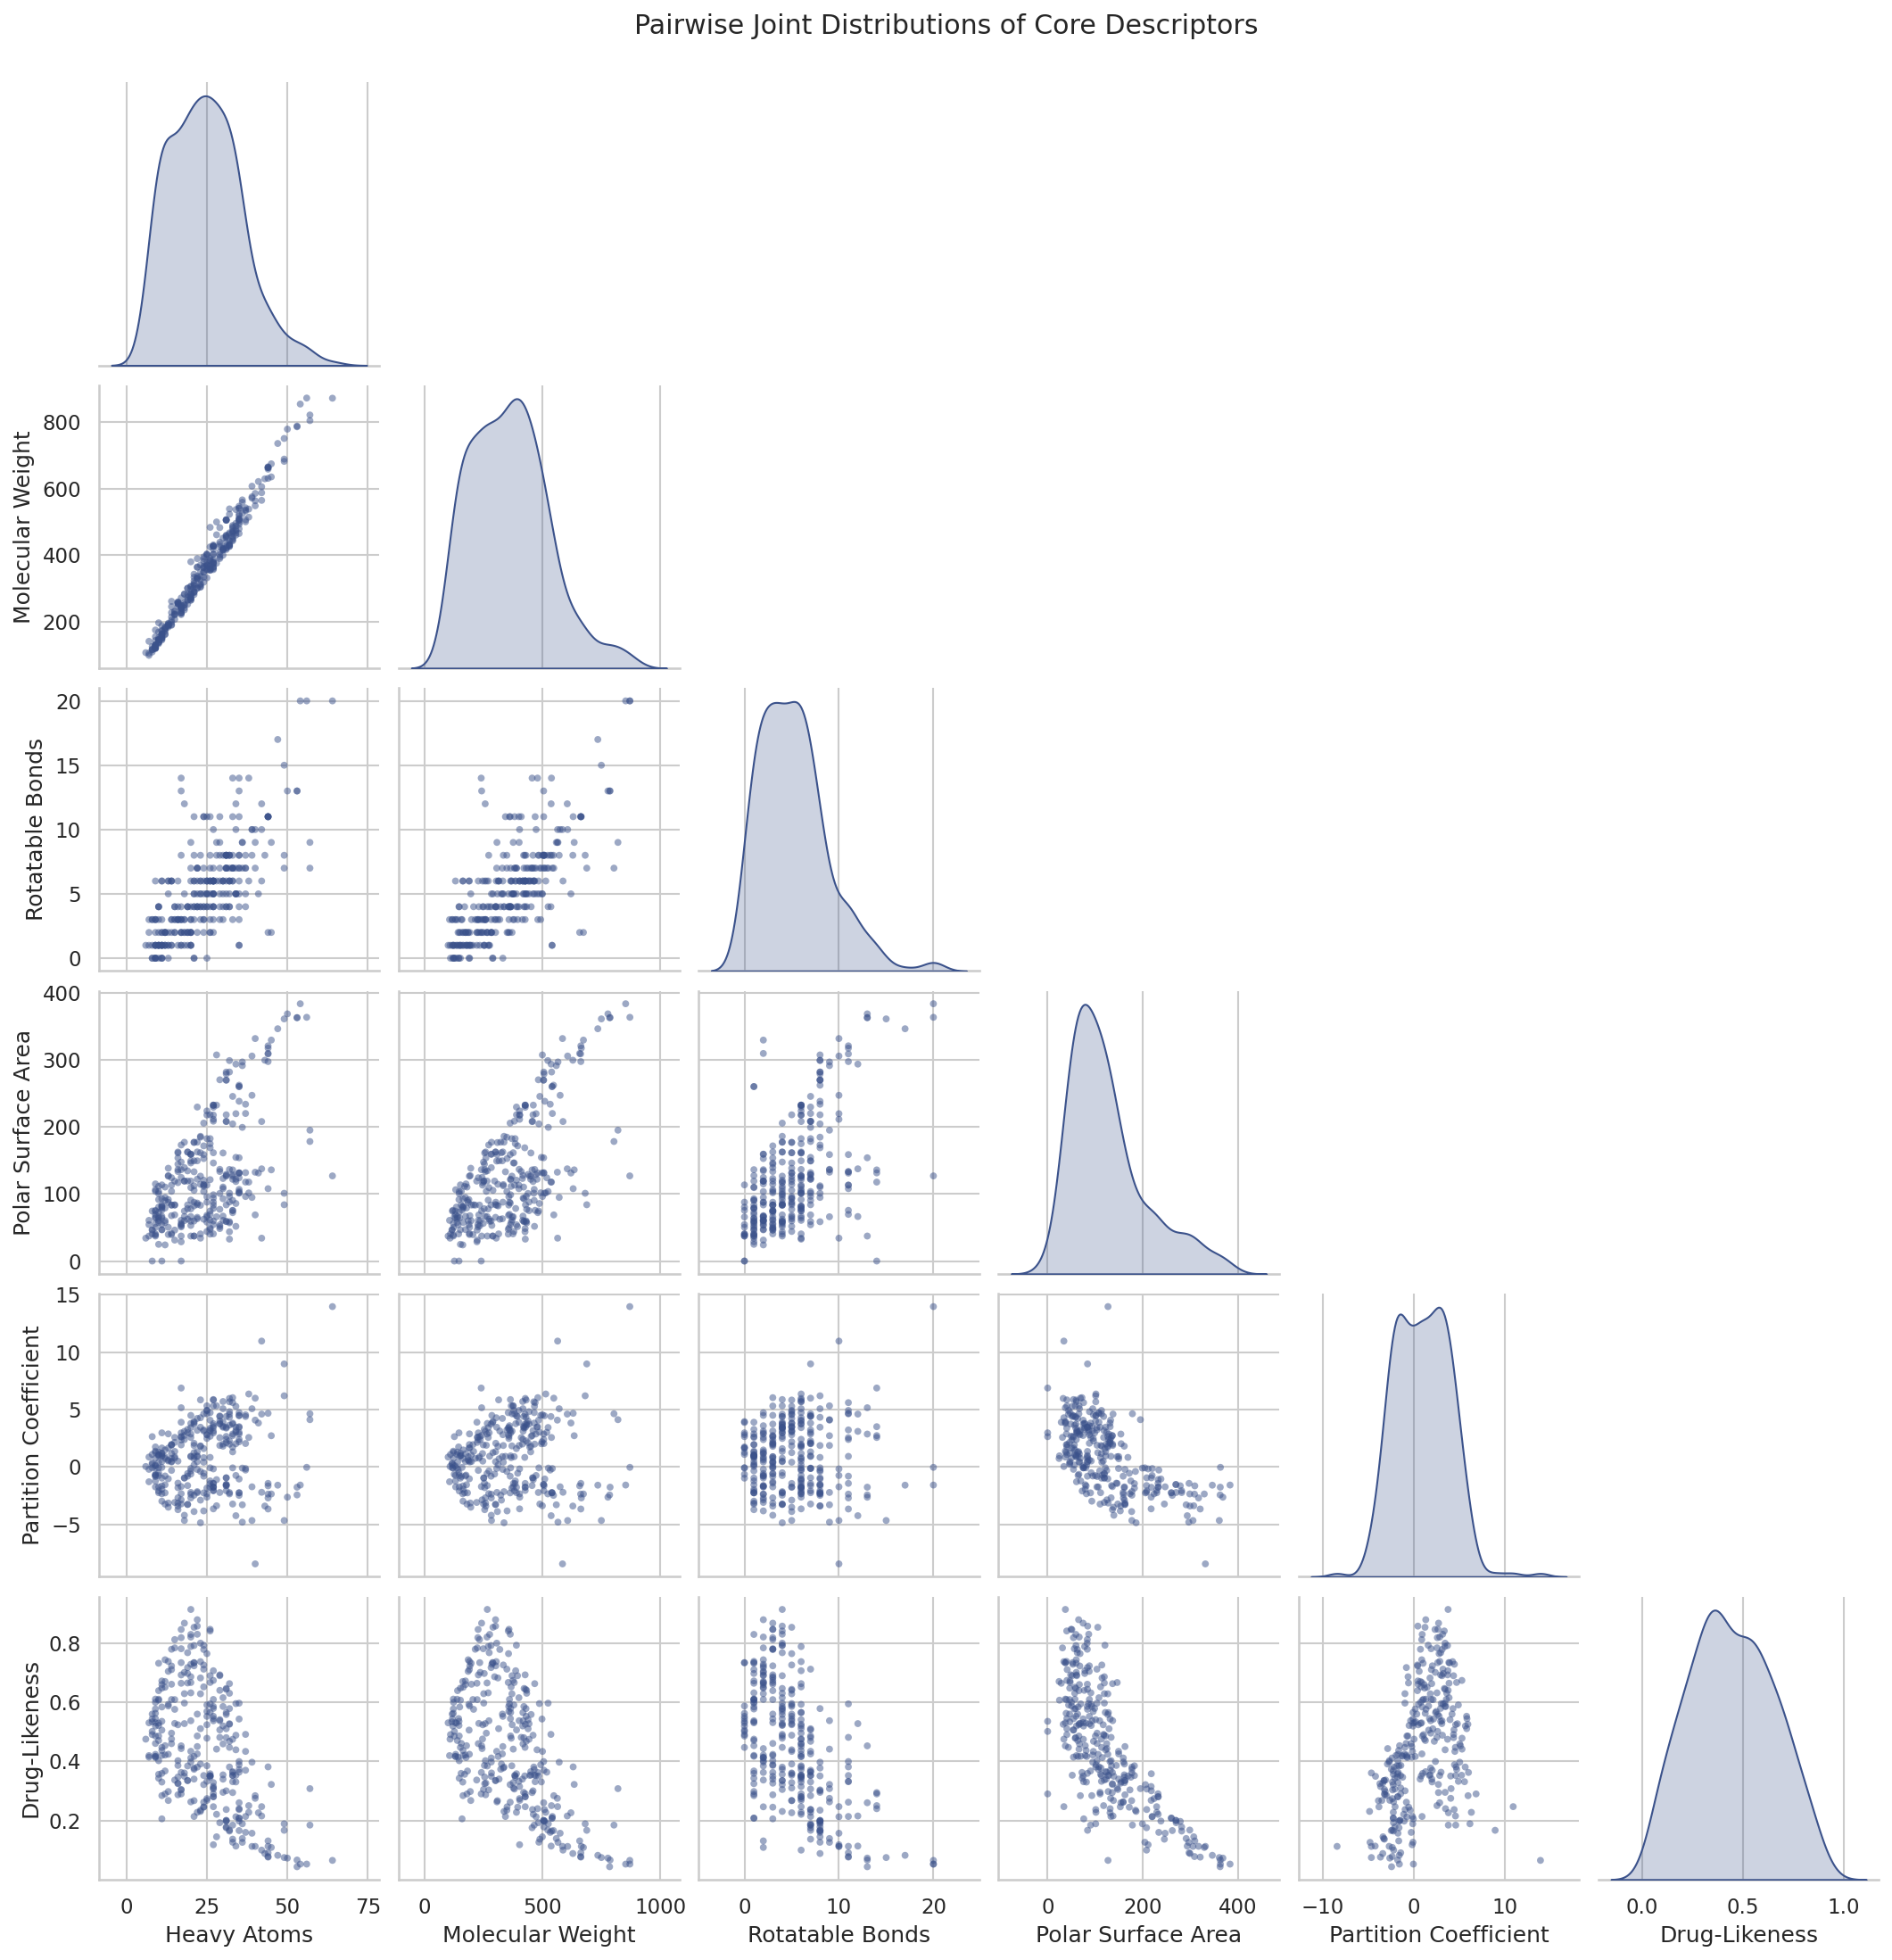
\includegraphics[width=\linewidth,height=0.78\textheight,keepaspectratio]{media/media/image38.png}
\caption[Joint distributions of six core descriptors]{Pairwise joint distributions of six core descriptors with kernel-density estimates on the diagonal}\label{fig:appendix-dataset-6}
\end{figure}

\hypertarget{principal-component-analysis-chemical-space}{%
\section{Principal-Component Analysis --- Chemical Space}\label{principal-component-analysis-chemical-space}}

To summarise this correlated space, a principal-component analysis was run on the sixteen standardised ligand descriptors. Two components already capture roughly two-thirds of the variance (PC1 \ensuremath{\approx} 45\%, PC2 \ensuremath{\approx} 23\%) and four reach about 81\% (Figure~\ref{fig:appendix-dataset-7}). Only a few underlying factors govern the set's diversity. The first component is a size-and-polarity axis. Heavy-atom count, molecular weight, hydrogen-bond acceptors and donors, polar surface area, heteroatom and stereocentre counts all load strongly and positively, while QED loads strongly negatively. Moving along PC1 therefore trades rising size, polarity and complexity against falling drug-likeness. The second component separates flat, lipophilic, aromatic, halogenated scaffolds (positive loadings on aromatic rings, cLogP, ring count and halogen count) from saturated, sp\textsuperscript{3}-rich, hydrogen-bond-donating ones. The minor components capture halogenation and element diversity (PC3) and net formal charge (PC4). The per-ligand difficulty of reproducing the crystal pose, overlaid on the score plot, rises towards positive PC1 (Figure~\ref{fig:appendix-dataset-8}). That identifies molecular size and flexibility, not aromatic or lipophilic character, as the dominant driver of docking difficulty.

\begin{figure}[!htbp]
\centering
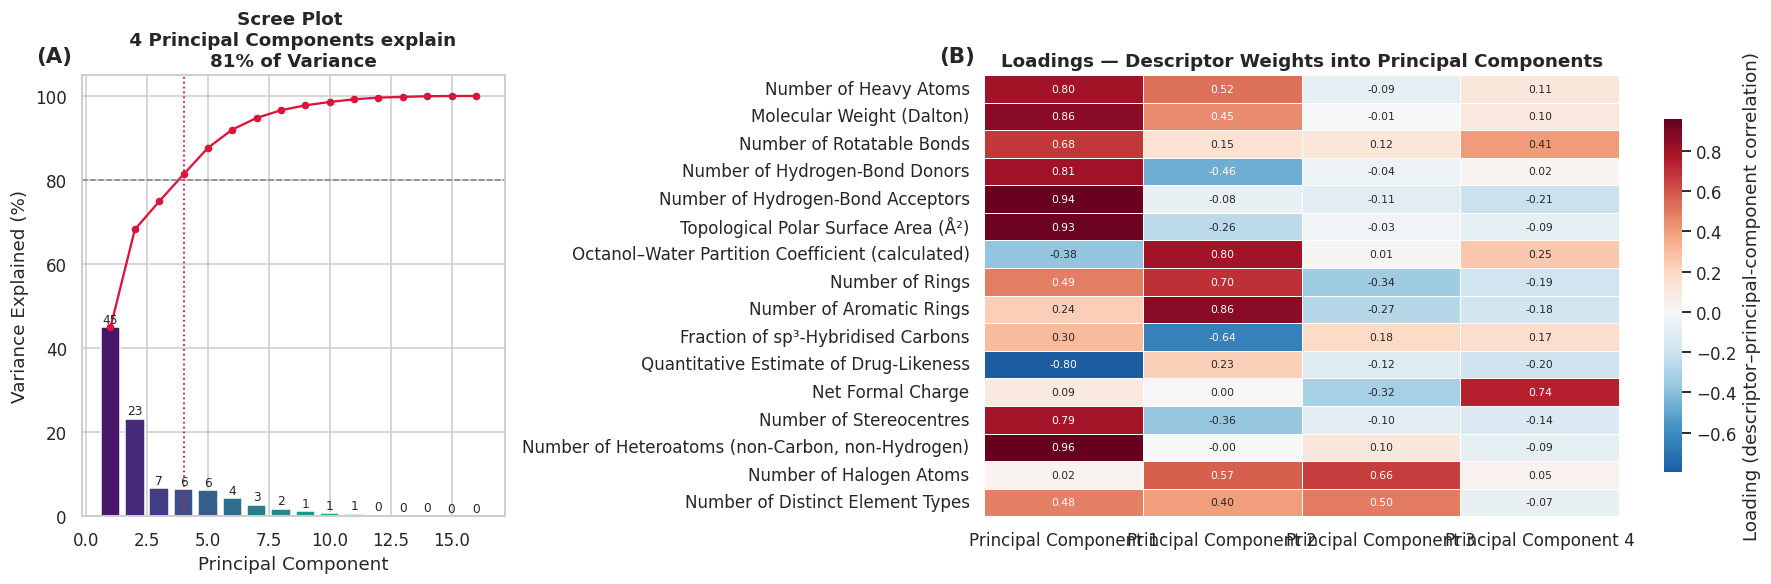
\includegraphics[width=\linewidth,height=0.78\textheight,keepaspectratio]{media/media/image39.png}
\caption[Principal Component Analysis of the Ligand Descriptors]{Principal component analysis of the standardised ligand descriptors. Scree plot of explained variance (A) and component loadings (B), where each cell is the correlation between a descriptor and a component}\label{fig:appendix-dataset-7}
\end{figure}

\begin{figure}[!htbp]
\centering

\includegraphics[width=\linewidth,height=0.78\textheight,keepaspectratio]{media/media/image40.png}
\caption[PCA biplot and score plot]{PCA biplot with descriptor loadings (A) and PC scores coloured by conformer-generation difficulty (B). The three experimental Orai1 ligands are projected into the same space}\label{fig:appendix-dataset-8}
\end{figure}

\hypertarget{receptor-profile}{%
\section{Receptor Profile}\label{receptor-profile}}

The receptor side is equally varied (Figure~\ref{fig:appendix-dataset-9}). A typical complex resolves 472 residues (interquartile range 306 to 778) and is a monomer or dimer. The distribution has a long tail of large multi-chain assemblies running to forty chains and several thousand residues. In the deposited source structures, 89\% of the complexes retain at least one cofactor or hetero-component, although receptor preparation removed most cofactors before docking. Ligand size is essentially independent of receptor size. Small ligands are docked into both small and very large pockets, and receptor dimensions cannot act as a confounding shortcut.

\begin{figure}[!htbp]
\centering

\includegraphics[width=\linewidth,height=0.78\textheight,keepaspectratio]{media/media/image41.png}
\caption[Receptor profile]{Receptor profile. Resolved residues, chains per complex, distinct cofactor types and ligand-versus-receptor size}\label{fig:appendix-dataset-9}
\end{figure}

\hypertarget{conformer-generation-difficulty}{%
\section{Conformer-Generation Difficulty}\label{conformer-generation-difficulty}}

The single ETKDGv3 + UFF starting conformer supplied with each ligand gives a lower-bound estimate of how much a docking engine must reshape the ligand to recover the crystal conformation. The best-fit (Kabsch) symmetry-corrected RMSD between this start conformer and the deposited reference instance of the crystallographic pose is computed after optimal superposition, so it isolates conformational difference from placement. It is a property of the start conformer and is not re-taken against the nearest copy. The median is 1.56\angstrom{}, and only 65\% of conformers fall within 2\angstrom{} of the crystal conformation (Figure~\ref{fig:appendix-dataset-10}). This quantity is not comparable with the in-place recovery threshold used in the Results, which does not superpose. This deviation grows steadily with rotatable-bond count (r = +0.75) and heavy-atom count (r = +0.80). The deviation quantifies the search burden and confirms that ligand size and flexibility are the set's principal sources of difficulty.

\begin{figure}[!htbp]
\centering

\includegraphics[width=\linewidth,height=0.78\textheight,keepaspectratio]{media/media/image42.png}
\caption[Conformer-generation difficulty]{Conformer-generation difficulty. The best-fit start-conformer-to-crystal RMSD distribution (A) and its dependence on rotatable bonds (B) and heavy-atom count (C)}\label{fig:appendix-dataset-10}
\end{figure}

\hypertarget{contrast-with-the-functionally-tested-ligands}{%
\section{Contrast with the Functionally Tested Ligands}\label{contrast-with-the-functionally-tested-ligands}}

The three modulators entered the pipeline as externally supplied optimised geometries. No conformer search was run to prepare them, and the program and level of theory behind that optimisation were not recorded and are not reconstructed here, in the same way that the receptor model\textquotesingle s build provenance is not. The docked 2abp-NH2 carries the InChIKey BLZVCIGGICSWIG-UHFFFAOYSA-N, which is native 2-APB in its neutral form. The docked Synta-66 carries GFEIWXNLDKUWIK-UHFFFAOYSA-N and the docked GSK-7975A carries CPYTVBALBFSXSH-UHFFFAOYSA-N. Both match the published identifiers for those compounds. The GSK-7975A key is that of the neutral phenol, and the phenolate anion prepared alongside it carries CPYTVBALBFSXSH-UHFFFAOYSA-M. The geometry-optimised Orai1 ligands were characterised with the identical descriptor pipeline and projected onto the same chemical-space maps for comparison. Unlike the benchmark complexes, these compounds are experimental and carry no crystallographic reference pose, so their binding modes must be predicted. Their physicochemical profile is markedly narrower and more lead-like than the benchmark set (Table~\ref{tab:appendix-orai-descriptors}). The three ligands have molecular weights of 225 to 397 Da, at most 28 heavy atoms, four to five rotatable bonds, one or two hydrogen-bond donors and polar surface areas below 68\angstrom{}\textsuperscript{2}. All three pass Lipinski's rule of five with zero violations and show QED values of roughly 0.65 to 0.76 (above the benchmark median of 0.43). Across the distribution figures the three experimental ligands consistently land on the small, drug-like, aromatic-lipophilic side of every attribute. In the principal-component projection they cluster at negative PC1 and positive PC2, the compact, lead-like, comparatively easy-to-reproduce corner of the benchmark's chemical space.

\scriptsize
\begin{longtable}[]{@{}
  >{\raggedright\arraybackslash}p{(\columnwidth - 18\tabcolsep) * \real{0.1350}}
  >{\raggedright\arraybackslash}p{(\columnwidth - 18\tabcolsep) * \real{0.2150}}
  >{\raggedright\arraybackslash}p{(\columnwidth - 18\tabcolsep) * \real{0.0850}}
  >{\raggedright\arraybackslash}p{(\columnwidth - 18\tabcolsep) * \real{0.0750}}
  >{\raggedright\arraybackslash}p{(\columnwidth - 18\tabcolsep) * \real{0.0700}}
  >{\raggedright\arraybackslash}p{(\columnwidth - 18\tabcolsep) * \real{0.0700}}
  >{\raggedright\arraybackslash}p{(\columnwidth - 18\tabcolsep) * \real{0.0900}}
  >{\raggedright\arraybackslash}p{(\columnwidth - 18\tabcolsep) * \real{0.0900}}
  >{\raggedright\arraybackslash}p{(\columnwidth - 18\tabcolsep) * \real{0.0800}}
  >{\raggedright\arraybackslash}p{(\columnwidth - 18\tabcolsep) * \real{0.0800}}@{}}
\caption[Orai1 Ligand Physicochemical Descriptors]{Physicochemical Descriptors of the Geometry-Optimised Experimental Orai1 Ligands, as Docked and Analysed. All three were docked as neutral species. This table carries the full descriptor set for the experimental ligands, and the pharmacology of each is given in Table~\ref{tab:appendix-orai-pharmacology}}\label{tab:appendix-orai-descriptors}\tabularnewline
\toprule\noalign{}
{\raggedright \textbf{Ligand}} & {\raggedright \textbf{Formula}} & {\raggedright \textbf{MW (Da)}} & \shortstack[l]{\textbf{Heavy}\\\textbf{atoms}\strut} & \shortstack[l]{\textbf{Rot.}\\\textbf{bonds}\strut} & \shortstack[l]{\textbf{Arom.}\\\textbf{rings}\strut} & {\raggedright \textbf{HBD / HBA}} & {\raggedright \textbf{TPSA (\angstrom{}\textsuperscript{2})}} & {\raggedright \textbf{cLogP}} & \shortstack[l]{\textbf{Ro5}\\\textbf{viol.}\strut} \\
\midrule\noalign{}
\endfirsthead
\caption[]{Physicochemical Descriptors of the Geometry-Optimised Experimental Orai1 Ligands (continued)}\tabularnewline
\toprule\noalign{}
{\raggedright \textbf{Ligand}} & {\raggedright \textbf{Formula}} & {\raggedright \textbf{MW (Da)}} & \shortstack[l]{\textbf{Heavy}\\\textbf{atoms}\strut} & \shortstack[l]{\textbf{Rot.}\\\textbf{bonds}\strut} & \shortstack[l]{\textbf{Arom.}\\\textbf{rings}\strut} & {\raggedright \textbf{HBD / HBA}} & {\raggedright \textbf{TPSA (\angstrom{}\textsuperscript{2})}} & {\raggedright \textbf{cLogP}} & \shortstack[l]{\textbf{Ro5}\\\textbf{viol.}\strut} \\
\midrule\noalign{}
\endhead
\bottomrule\noalign{}
\endlastfoot
2abp-NH2 & C\textsubscript{14}H\textsubscript{16}BNO & 225.1 & 17 & 5 & 2 & 1 / 2 & 35.3 & 0.77 & 0 \\
Synta-66 & C\textsubscript{20}H\textsubscript{17}FN\textsubscript{2}O\textsubscript{3} & 352.4 & 26 & 5 & 3 & 1 / 4 & 60.5 & 4.16 & 0 \\
GSK-7975A (neutral) & C\textsubscript{18}H\textsubscript{12}F\textsubscript{5}N\textsubscript{3}O\textsubscript{2} & 397.3 & 28 & 4 & 3 & 2 / 4 & 67.2 & 4.19 & 0 \\
\end{longtable}
\normalsize
% PROVENANCE (updated 2026-08-16). The GSK-7975A row of this table and of Table 3 in the
% main text describes the NEUTRAL species, so the descriptor source is
% Data/Ligands/JKU/pdbqt/gsk7975a-deprot-as-neutral-OPT.sdf (RDKit reads it as
% C18H12F5N3O2, 397.3 Da, 28 heavy atoms, 2 HBD, TPSA 67.2; the byte-different
% gsk7975a-prot-OPT.sdf gives the identical descriptor set). Do NOT regenerate from
% gsk7975a-deprot-OPT.sdf: that file is the -1 phenolate (C18H11F5N3O2-, 396.3 Da, 1 HBD,
% TPSA 70.0) and is a DIFFERENT species from the one reported here. The earlier note on
% this line named the deprotonated file and is superseded.
% Other two rows: 2abp-NH2/2-APB from 2abp-nh2-OPT.sdf, C14H16BNO 225.1 Da/17 heavy atoms;
% Synta-66 from Synta-66-OPT-Singlet.sdf, C20H17FN2O3 (no S) 352.4 Da/26 heavy atoms.
% BASIS CORRECTION 2026-08-19: the rotatable-bond column of this table and of Table 3 was
% computed on HYDROGEN-EXPLICIT molecules, because _load_jku_mol passes sanitize=False, which
% suppresses RDKit's implicit RemoveHs, while the benchmark loader (Chem.MolFromMolFile with the
% default removeHs=True) is hydrogen-suppressed. The two tables were therefore on different bases.
% Recomputed on Chem.RemoveHs: 2abp-NH2 6->5, Synta-66 7->5, GSK-7975A 5->4. The surplus bonds were
% the terminal C-NH2, phenol C-OH and methoxy O-CH3 bonds the standard descriptor excludes.
% VALIDATED: every OTHER descriptor in this table is identical on both bases (MW, heavy atoms,
% HBD/HBA, TPSA, cLogP, QED), and gsk7975a-prot-OPT.sdf and gsk7975a-deprot-as-neutral-OPT.sdf
% give the identical descriptor set on both bases. Across the full 16-descriptor PCA feature set
% exactly one further descriptor is basis-dependent, n_element_types (5 with H, 4 without), which
% is not printed in any table. Correcting both moves the three JKU points in the PCA biplot by
% 0.36 to 0.43 units against benchmark PC1/PC2 standard deviations of 2.68 and 1.93, about 0.13
% sd, so all three stay at negative PC1 and positive PC2 and no interpretation changes. The
% notebook loader _load_jku_mol was fixed on 2026-08-19 to return Chem.RemoveHs(m). All ten
% appendix chemical-space figures WERE then re-rendered and re-embedded as image33 to image42.
% CORRECTED 2026-08-19: the earlier note on these two lines claimed the figures were not
% re-rendered because the shift is invisible at figure scale. Both halves are false. Every one
% of image33 to image42 is md5-identical to its PoseBusters_Benchmark_Analysis/figures/
% counterpart, and the shift is NOT invisible in Figure 35. Collapsing the Synta-66/GSK-7975A
% rotatable-bond gap from 2 to 1 dropped |dy|/yspan to 0.0351, under the 0.04 coincidence
% tolerance of overlay_jku_points, so panel (A) now fans the two markers apart by 0.035*xspan =
% 2.93 heavy atoms each way and draws them in reversed left-to-right order. The Figure 35
% caption was corrected to match. Verified by re-running notebook cell 87264e87 on the post-fix
% basis, which reproduces image37.png byte-for-byte (md5 429a8a25b546263a09f36d1dcb8d5e86).
% Identity note: docked 2abp-NH2 InChIKey BLZVCIGGICSWIG-UHFFFAOYSA-N == native 2-APB
% (neutral form), PubChem CID 1598 -- it is the same molecule, not a distinct analogue.

\hypertarget{suitability-of-the-dataset}{%
\section{Suitability of the Dataset}\label{suitability-of-the-dataset}}

This contrast makes the PoseBusters benchmark a sound calibration anchor. It brackets and clearly exceeds the chemical and structural complexity of the experimental Orai1 ligands, being larger, more polar, more flexible and more diverse, and it sets a harder conformer-search problem. That argument runs on the ligand axis alone. On the receptor axis the two settings are not matched, because every calibration complex is re-docked into its own cognate crystal receptor whereas the Orai1 arm docks into non-cognate molecular-dynamics snapshots of a homology-modelled membrane channel. Docking benchmarks curate self-docking and cross-docking as separate sets because the cognate case is the less realistic of the two \cite{ref012}, and cross-docking accuracy depends further on which non-cognate receptor is chosen \cite{ref033}. The size of that penalty is not measured here. The calibration figures are therefore treated as an upper bound on Orai1 performance rather than as a prediction. That treatment is a stated assumption and not a measured result. Calibrating the three pipelines on it therefore establishes their performance over a range that comfortably contains the smaller, lead-like Orai1 compounds, and it does so against experimentally resolved poses that the experimental dataset itself cannot supply.

\hypertarget{ranking-recovery-statistics}{%
\chapter{Ranking-Recovery Statistics}\label{ranking-recovery-statistics}}

These tables carry both DiffDock refiners, so the smina arm the Results select is printed beside the gnina one. Table~\ref{tab:appendix-top-k-recovery} prints both gates, near-native placement alone and the validity-aware conjunction the Results use, and the two arms stand at 45.2\% against 45.5\% rank-1 on the first and at 43.6\% against 44.2\% on the second. Every paired test in this chapter is taken on the near-native gate alone. The following tables give depth-resolved statistics for the variants displayed below. Recovery is reported for k = 1, 5, 10 and 15 over the N = 303 calibration complexes. Percentages are complex-level recovery rates and bracketed intervals are Wilson 95\% confidence intervals. Paired comparisons use McNemar\textquotesingle s exact test with Holm correction. The eight prespecified comparisons form two families of sixteen, each taken at the four depths and each corrected on its own. The between-tool family holds the four cross-tool comparisons of Table~\ref{tab:appendix-cross-tool-mcnemar} and the within-tool family holds the four optimisation contrasts of Table~\ref{tab:appendix-refinement-mcnemar}. The two ask different questions, and pooling them would let one tool\textquotesingle s optimisation row change every cross-tool verdict for no methodological reason. Significance is marked as * p \textless{} 0.05, ** p \textless{} 0.01 and *** p \textless{} 0.001, and ns denotes not significant. The between-tool family is computed on the gnina-rescored AutoDock Vina arm that the recovery tables below display, ranked by that arm\textquotesingle s own rescored order. Every corrected p value in this chapter therefore refers to a variant printed here. The four between-tool comparisons, each taken on the near-native endpoint, are AutoDock Vina + gnina against DiffDock (raw), AutoDock Vina + gnina against DiffDock (gnina-opt), DiffDock (gnina-opt) against EquiBind (gnina-opt), and AutoDock Vina + gnina against EquiBind (gnina-opt). The four within-tool contrasts, on the same endpoint, are AutoDock Vina against AutoDock Vina + gnina, DiffDock (raw) against DiffDock + smina, DiffDock (raw) against DiffDock (gnina-opt), and EquiBind (raw) against EquiBind (gnina-opt). The validity-aware endpoint is not part of the family, because the validity-aware set is a strict subset of the near-native set. Its gap is reported as an effect size in Table~\ref{tab:appendix-accurate-invalid} rather than tested. Every table in this chapter is computed on the blind whole-protein run that supplies the Results chapter.

\begingroup
\scriptsize
\setlength{\tabcolsep}{2pt}
\begin{longtable}[]{@{}
  >{\raggedright\arraybackslash}p{(\columnwidth - 6\tabcolsep) * \real{0.2500}}
  >{\raggedright\arraybackslash}p{(\columnwidth - 6\tabcolsep) * \real{0.2500}}
  >{\raggedright\arraybackslash}p{(\columnwidth - 6\tabcolsep) * \real{0.2500}}
  >{\raggedright\arraybackslash}p{(\columnwidth - 6\tabcolsep) * \real{0.2500}}@{}}
\caption[Top-k Recovery with Wilson Intervals]{Top-k Recovery with Wilson 95\% Confidence Intervals}\label{tab:appendix-top-k-recovery}\tabularnewline
\toprule\noalign{}
{\raggedright \textbf{Variant}} & {\raggedright \textbf{k}} & {\raggedright \textbf{Near-native\% {[}95\% CI{]}}} & {\raggedright \textbf{Validity-aware\% {[}95\% CI{]}}} \\
\midrule\noalign{}
\endfirsthead
\caption[]{Top-k Recovery with Wilson 95\% Confidence Intervals (continued)}\tabularnewline
\toprule\noalign{}
{\raggedright \textbf{Variant}} & {\raggedright \textbf{k}} & {\raggedright \textbf{Near-native\% {[}95\% CI{]}}} & {\raggedright \textbf{Validity-aware\% {[}95\% CI{]}}} \\
\midrule\noalign{}
\endhead
\bottomrule\noalign{}
\endlastfoot
AutoDock Vina (raw) & 1 & 43.2 {[}37.8, 48.9{]} & 42.9 {[}37.5, 48.5{]} \\
 & 5 & 56.4 {[}50.8, 61.9{]} & 56.1 {[}50.5, 61.6{]} \\
 & 10 & 62.7 {[}57.1, 68.0{]} & 62.7 {[}57.1, 68.0{]} \\
 & 15 & 65.3 {[}59.8, 70.5{]} & 65.3 {[}59.8, 70.5{]} \\
AutoDock Vina + gnina & 1 & 49.8 {[}44.2, 55.4{]} & 49.2 {[}43.6, 54.8{]} \\
 & 5 & 67.3 {[}61.9, 72.4{]} & 66.0 {[}60.5, 71.1{]} \\
 & 10 & 70.0 {[}64.6, 74.9{]} & 69.0 {[}63.6, 73.9{]} \\
 & 15 & 71.3 {[}66.0, 76.1{]} & 70.3 {[}64.9, 75.2{]} \\
DiffDock (raw) & 1 & 43.6 {[}38.1, 49.2{]} & 22.1 {[}17.8, 27.1{]} \\
 & 5 & 50.2 {[}44.6, 55.8{]} & 30.4 {[}25.5, 35.8{]} \\
 & 10 & 52.1 {[}46.5, 57.7{]} & 32.7 {[}27.6, 38.1{]} \\
 & 15 & 52.8 {[}47.2, 58.4{]} & 34.0 {[}28.9, 39.5{]} \\
DiffDock + smina & 1 & 45.2 {[}39.7, 50.8{]} & 43.6 {[}38.1, 49.2{]} \\
 & 5 & 54.1 {[}48.5, 59.6{]} & 52.8 {[}47.2, 58.4{]} \\
 & 10 & 57.8 {[}52.1, 63.2{]} & 56.8 {[}51.1, 62.2{]} \\
 & 15 & 60.1 {[}54.5, 65.4{]} & 59.1 {[}53.5, 64.5{]} \\
DiffDock + gnina & 1 & 45.5 {[}40.0, 51.2{]} & 44.2 {[}38.7, 49.9{]} \\
 & 5 & 54.1 {[}48.5, 59.6{]} & 53.1 {[}47.5, 58.7{]} \\
 & 10 & 57.1 {[}51.5, 62.5{]} & 56.1 {[}50.5, 61.6{]} \\
 & 15 & 59.4 {[}53.8, 64.8{]} & 58.4 {[}52.8, 63.8{]} \\
EquiBind (raw) & 1 & 1.3 {[}0.5, 3.3{]} & 0.7 {[}0.2, 2.4{]} \\
 & 5 & 3.0 {[}1.6, 5.5{]} & 0.7 {[}0.2, 2.4{]} \\
 & 10 & 4.0 {[}2.3, 6.8{]} & 0.7 {[}0.2, 2.4{]} \\
 & 15 & 5.9 {[}3.8, 9.2{]} & 0.7 {[}0.2, 2.4{]} \\
EquiBind + gnina & 1 & 19.5 {[}15.4, 24.3{]} & 18.8 {[}14.8, 23.6{]} \\
 & 5 & 26.1 {[}21.5, 31.3{]} & 25.1 {[}20.5, 30.3{]} \\
 & 10 & 28.4 {[}23.6, 33.7{]} & 27.4 {[}22.7, 32.7{]} \\
 & 15 & 28.4 {[}23.6, 33.7{]} & 27.4 {[}22.7, 32.7{]} \\
\end{longtable}
\endgroup

\begingroup
\scriptsize
\setlength{\tabcolsep}{2pt}
\begin{longtable}[]{@{}
  >{\raggedright\arraybackslash}p{(\columnwidth - 12\tabcolsep) * \real{0.1429}}
  >{\raggedright\arraybackslash}p{(\columnwidth - 12\tabcolsep) * \real{0.1429}}
  >{\raggedright\arraybackslash}p{(\columnwidth - 12\tabcolsep) * \real{0.1429}}
  >{\raggedright\arraybackslash}p{(\columnwidth - 12\tabcolsep) * \real{0.1429}}
  >{\raggedright\arraybackslash}p{(\columnwidth - 12\tabcolsep) * \real{0.1429}}
  >{\raggedright\arraybackslash}p{(\columnwidth - 12\tabcolsep) * \real{0.1429}}
  >{\raggedright\arraybackslash}p{(\columnwidth - 12\tabcolsep) * \real{0.1429}}@{}}
\caption[Optimisation Effect on Cumulative Top-k Recovery]{Within-Tool Optimisation Effect on Cumulative Top-k Near-Native Recovery}\label{tab:appendix-refinement-mcnemar}\tabularnewline
\toprule\noalign{}
{\raggedright \textbf{Tool}} & {\raggedright \textbf{k}} & {\raggedright \textbf{raw\% \ensuremath{\rightarrow} opt\%}} & {\raggedright \textbf{discordant (raw-only / opt-only)}} & {\raggedright \textbf{p (raw)}} & {\raggedright \textbf{p (Holm)}} & {\raggedright \textbf{sig}} \\
\midrule\noalign{}
\endfirsthead
\caption[]{Raw-to-gnina Optimisation Effect on Cumulative Top-k Near-Native Recovery (continued)}\tabularnewline
\toprule\noalign{}
{\raggedright \textbf{Tool}} & {\raggedright \textbf{k}} & {\raggedright \textbf{raw\% \ensuremath{\rightarrow} opt\%}} & {\raggedright \textbf{discordant (raw-only / opt-only)}} & {\raggedright \textbf{p (raw)}} & {\raggedright \textbf{p (Holm)}} & {\raggedright \textbf{sig}} \\
\midrule\noalign{}
\endhead
\bottomrule\noalign{}
\endlastfoot
AutoDock Vina + gnina & 1 & 43.2 \ensuremath{\rightarrow} 49.8 & 19 / 39 & 0.0119 & 0.0596 & ns \\
 & 5 & 56.4 \ensuremath{\rightarrow} 67.3 & 3 / 36 & \textless1e-4 & \textless1e-4 & *** \\
 & 10 & 62.7 \ensuremath{\rightarrow} 70.0 & 3 / 25 & \textless1e-4 & 3.0e-4 & *** \\
 & 15 & 65.3 \ensuremath{\rightarrow} 71.3 & 1 / 19 & \textless1e-4 & 4.0e-4 & *** \\
DiffDock + smina & 1 & 43.6 \ensuremath{\rightarrow} 45.2 & 5 / 10 & 0.302 & 0.476 & ns \\
 & 5 & 50.2 \ensuremath{\rightarrow} 54.1 & 5 / 17 & 0.0169 & 0.0676 & ns \\
 & 10 & 52.1 \ensuremath{\rightarrow} 57.8 & 5 / 22 & 0.0015 & 0.0106 & * \\
 & 15 & 52.8 \ensuremath{\rightarrow} 60.1 & 5 / 27 & 1.1e-4 & 0.0010 & ** \\
DiffDock + gnina & 1 & 43.6 \ensuremath{\rightarrow} 45.5 & 6 / 12 & 0.238 & 0.476 & ns \\
 & 5 & 50.2 \ensuremath{\rightarrow} 54.1 & 5 / 17 & 0.0169 & 0.0676 & ns \\
 & 10 & 52.1 \ensuremath{\rightarrow} 57.1 & 5 / 20 & 0.0041 & 0.0245 & * \\
 & 15 & 52.8 \ensuremath{\rightarrow} 59.4 & 5 / 25 & 3.2e-4 & 0.0026 & ** \\
EquiBind + gnina & 1 & 1.3 \ensuremath{\rightarrow} 19.5 & 2 / 57 & \textless1e-4 & \textless1e-4 & *** \\
 & 5 & 3.0 \ensuremath{\rightarrow} 26.1 & 2 / 72 & \textless1e-4 & \textless1e-4 & *** \\
 & 10 & 4.0 \ensuremath{\rightarrow} 28.4 & 1 / 75 & \textless1e-4 & \textless1e-4 & *** \\
 & 15 & 5.9 \ensuremath{\rightarrow} 28.4 & 1 / 69 & \textless1e-4 & \textless1e-4 & *** \\
\multicolumn{7}{@{}p{\dimexpr\columnwidth-12\tabcolsep\relax}@{}}{\footnotesize%
Recovery here is the cumulative best-of-top-\emph{k} complex rate, in which a complex counts when \emph{any} of its top-\emph{k} poses is near-native. The four contrasts are within-tool and form their own Holm family of sixteen, corrected separately from the between-tool family of Table~\ref{tab:appendix-cross-tool-mcnemar}. The two ask different questions, and pooling them would let one tool\textquotesingle s optimisation row change every cross-tool verdict for no methodological reason. The operation itself differs by tool, so these are not three measurements of one mechanism. AutoDock Vina\textquotesingle s gnina step both minimises each pose and re-orders the pool on CNN affinity, so its gain mixes geometry with ranking and this design cannot separate them. For DiffDock the top-\emph{k} pool is the same set of confidence-ranked poses before and after refinement, so its gain is geometry repair alone, accumulated across ranks by the best-of-top-\emph{k} union rather than produced by any re-ordering. Re-ordering was measured separately on the same 303 complexes and does not help, since ranking the unrefined poses by their refined affinity rather than by confidence nominates a near-native rank-1 pose for 41.6\% of complexes with gnina and 41.6\% with smina, against the 43.6\% of the confidence order. EquiBind has no native ranking, so its gnina variant is additionally re-ranked by gnina affinity and its gain is the two effects together. Read across the tools, the size of the gain runs inverse to how good the raw poses already were. EquiBind starts at 1.3\% and gains more than eighteen points at rank-1, AutoDock Vina starts at 43.2\% and gains nearly seven, DiffDock starts at 43.6\% and gains two. At the top-15 depth the ordering of the optimised arms, 71.3\% for AutoDock Vina against 60.1\% and 59.4\% for the two DiffDock refiners and 28.4\% for EquiBind, repeats the ordering of the raw arms, so optimisation narrows the gaps without reversing them. The two DiffDock refiners are within one point of each other, reaching 60.1\% and 59.4\% at top-15 by way of 27 and 25 recovered complexes, which is why the Results chapter treats the choice between them as immaterial.} \\
\end{longtable}
\endgroup

\begingroup
\scriptsize
\setlength{\tabcolsep}{2pt}
\begin{longtable}[]{@{}
  >{\raggedright\arraybackslash}p{(\columnwidth - 14\tabcolsep) * \real{0.1400}}
  >{\raggedright\arraybackslash}p{(\columnwidth - 14\tabcolsep) * \real{0.2200}}
  >{\raggedright\arraybackslash}p{(\columnwidth - 14\tabcolsep) * \real{0.1067}}
  >{\raggedright\arraybackslash}p{(\columnwidth - 14\tabcolsep) * \real{0.1067}}
  >{\raggedright\arraybackslash}p{(\columnwidth - 14\tabcolsep) * \real{0.1067}}
  >{\raggedright\arraybackslash}p{(\columnwidth - 14\tabcolsep) * \real{0.1067}}
  >{\raggedright\arraybackslash}p{(\columnwidth - 14\tabcolsep) * \real{0.1066}}
  >{\raggedright\arraybackslash}p{(\columnwidth - 14\tabcolsep) * \real{0.1066}}@{}}
\caption[Fixed-Rank Optimisation Gain by Pose-Rank Band]{Fixed-Rank Optimisation Gain in Near-Native and Validity Rates by Pose-Rank Band}\label{tab:appendix-refinement-bands}\tabularnewline
\toprule\noalign{}
{\raggedright \textbf{Tool}} & {\raggedright \textbf{Criterion}} & {\raggedright \textbf{1--10 smina}} & {\raggedright \textbf{1--10 gnina}} & {\raggedright \textbf{11--20 smina}} & {\raggedright \textbf{11--20 gnina}} & {\raggedright \textbf{21--30 smina}} & {\raggedright \textbf{21--30 gnina}} \\
\midrule\noalign{}
\endfirsthead
\caption[]{Fixed-Rank Optimisation Gain in Near-Native and Validity Rates by Pose-Rank Band (continued)}\tabularnewline
\toprule\noalign{}
{\raggedright \textbf{Tool}} & {\raggedright \textbf{Criterion}} & {\raggedright \textbf{1--10 smina}} & {\raggedright \textbf{1--10 gnina}} & {\raggedright \textbf{11--20 smina}} & {\raggedright \textbf{11--20 gnina}} & {\raggedright \textbf{21--30 smina}} & {\raggedright \textbf{21--30 gnina}} \\
\midrule\noalign{}
\endhead
\bottomrule\noalign{}
\endlastfoot
DiffDock & near-native & +0.6 & +0.6 & +0.4 & +0.3 & +0.8 & +1.0 \\
DiffDock & PoseBusters-valid & +57 & +59 & +60 & +62 & +63 & +67 \\
DiffDock & near-native and PB-valid & +16.5 & +16.5 & +10.5 & +10.3 & +6.5 & +6.7 \\
EquiBind & near-native & +4.5 & +4.7 & +3.6 & +4.6 & +3.9 & +4.4 \\
EquiBind & PoseBusters-valid & +48 & +58 & +49 & +59 & +48 & +60 \\
EquiBind & near-native and PB-valid & +4.9 & +5.1 & +4.1 & +5.2 & +4.3 & +5.0 \\
\multicolumn{8}{@{}p{\dimexpr\columnwidth-14\tabcolsep\relax}@{}}{\footnotesize%
Entries are the change in the per-rank rate (percentage points) averaged within each pose-rank band, with every pose held at its own confidence rank for DiffDock or generation rank for EquiBind, so no re-ranking is involved. Every entry is computed on the blind whole-protein run that supplies the Results chapter, using the pose-count-weighted pooled rate within each band. The near-native gnina bands span 0.3 to 1.0 percentage points for DiffDock and 4.4 to 4.7 for EquiBind, and the smina bands span 0.4 to 0.8 and 3.6 to 4.5. The three bands partition ranks 1 to 30 with almost equal pose counts, so their mean reproduces the whole-run validity gain implied by Table~\ref{tab:results-pose-production}, namely +60 percentage points for DiffDock with smina and +63 with gnina, against 84.5\% and 87.1\% validity from a raw 24.4\%, and +48 and +59 for unguided EquiBind, against 51.3\% and 62.0\% from a raw 2.9\%. The derived near-native and PB-valid column is shown for context and is near-nativeness and validity by construction.} \\
\end{longtable}
\endgroup

Tables~\ref{tab:appendix-cross-tool-mcnemar} and~\ref{tab:appendix-accurate-invalid} provide the corresponding cross-tool recovery contrasts and the share of near-native complexes excluded by physical-invalidity screening.

\begingroup
\scriptsize
\setlength{\tabcolsep}{2pt}
\begin{longtable}[]{@{}
  >{\raggedright\arraybackslash}p{(\columnwidth - 8\tabcolsep) * \real{0.2000}}
  >{\raggedright\arraybackslash}p{(\columnwidth - 8\tabcolsep) * \real{0.2000}}
  >{\raggedright\arraybackslash}p{(\columnwidth - 8\tabcolsep) * \real{0.2000}}
  >{\raggedright\arraybackslash}p{(\columnwidth - 8\tabcolsep) * \real{0.2001}}
  >{\raggedright\arraybackslash}p{(\columnwidth - 8\tabcolsep) * \real{0.2001}}@{}}
\caption[Cross-Tool Comparisons of Near-Native Recovery]{Cross-Tool Comparisons of Near-Native Recovery}\label{tab:appendix-cross-tool-mcnemar}\tabularnewline
\toprule\noalign{}
{\raggedright \textbf{Comparison (near-native\%)}} & {\raggedright \textbf{k = 1}} & {\raggedright \textbf{k = 5}} & {\raggedright \textbf{k = 10}} & {\raggedright \textbf{k = 15}} \\
\midrule\noalign{}
\endfirsthead
\caption[]{Cross-Tool Comparisons of Near-Native Recovery (continued)}\tabularnewline
\toprule\noalign{}
{\raggedright \textbf{Comparison (near-native\%)}} & {\raggedright \textbf{k = 1}} & {\raggedright \textbf{k = 5}} & {\raggedright \textbf{k = 10}} & {\raggedright \textbf{k = 15}} \\
\midrule\noalign{}
\endhead
\bottomrule\noalign{}
\endlastfoot
AutoDock Vina + gnina versus DiffDock (raw) & 49.8 versus 43.6 & 67.3 versus 50.2 & 70.0 versus 52.1 & 71.3 versus 52.8 \\
AutoDock Vina + gnina versus DiffDock (gnina-opt) & 49.8 versus 45.5 & 67.3 versus 54.1 & 70.0 versus 57.1 & 71.3 versus 59.4 \\
DiffDock (gnina-opt) versus EquiBind (gnina-opt) & 45.5 versus 19.5 & 54.1 versus 26.1 & 57.1 versus 28.4 & 59.4 versus 28.4 \\
AutoDock Vina + gnina versus EquiBind (gnina-opt) & 49.8 versus 19.5 & 67.3 versus 26.1 & 70.0 versus 28.4 & 71.3 versus 28.4 \\
\multicolumn{5}{@{}p{\dimexpr\columnwidth-8\tabcolsep\relax}@{}}{\footnotesize%
Entries are complex-level near-native recovery percentages over the N = 303 calibration complexes, computed on the blind whole-protein run, and they match the near-native column of Table~\ref{tab:appendix-top-k-recovery}. These four contrasts are the between-tool Holm family of sixteen described at the head of this chapter, corrected separately from the within-tool family of Table~\ref{tab:appendix-refinement-mcnemar}. No significance marks are printed in the cells above, so the corrected results of those sixteen tests are given here. Both AutoDock contrasts against DiffDock are unresolved at rank-1 and significant at every deeper pool. Against DiffDock (raw) the Holm-corrected p runs 0.242 at k = 1 and then 1.2e-4, 6.5e-5 and 3.8e-5, and against DiffDock (gnina-opt) it runs 0.294 at k = 1 and then 0.0042, 0.0042 and 0.0071. The rank-1 result is an unresolved nominal lead rather than a tie, with AutoDock winning 77 complexes and losing 58 against DiffDock (raw) at an exact p of 0.12 before correction and winning 72 and losing 59 against DiffDock (gnina-opt). Both contrasts against EquiBind (gnina-opt) are significant at every depth, at a Holm-corrected p below 1e-12 throughout, so all eight of those tests clear the 0.001 threshold.} \\
\end{longtable}
\endgroup

\begingroup
\scriptsize
\setlength{\tabcolsep}{2pt}
\begin{longtable}[]{@{}
  >{\raggedright\arraybackslash}p{(\columnwidth - 8\tabcolsep) * \real{0.2000}}
  >{\raggedright\arraybackslash}p{(\columnwidth - 8\tabcolsep) * \real{0.2000}}
  >{\raggedright\arraybackslash}p{(\columnwidth - 8\tabcolsep) * \real{0.2000}}
  >{\raggedright\arraybackslash}p{(\columnwidth - 8\tabcolsep) * \real{0.2001}}
  >{\raggedright\arraybackslash}p{(\columnwidth - 8\tabcolsep) * \real{0.2001}}@{}}
\caption[Accurate-but-Invalid Share by Ranking Depth]{Accurate-but-Invalid Share by Ranking Depth}\label{tab:appendix-accurate-invalid}\tabularnewline
\toprule\noalign{}
{\raggedright \textbf{Variant}} & {\raggedright \textbf{k = 1}} & {\raggedright \textbf{k = 5}} & {\raggedright \textbf{k = 10}} & {\raggedright \textbf{k = 15}} \\
\midrule\noalign{}
\endfirsthead
\caption[]{Accurate-but-Invalid Share by Ranking Depth (continued)}\tabularnewline
\toprule\noalign{}
{\raggedright \textbf{Variant}} & {\raggedright \textbf{k = 1}} & {\raggedright \textbf{k = 5}} & {\raggedright \textbf{k = 10}} & {\raggedright \textbf{k = 15}} \\
\midrule\noalign{}
\endhead
\bottomrule\noalign{}
\endlastfoot
AutoDock Vina + gnina & 0.7 {[}0.2, 2.4{]} & 1.3 {[}0.5, 3.3{]} & 1.0 {[}0.3, 2.9{]} & 1.0 {[}0.3, 2.9{]} \\
DiffDock (raw) & 21.5 {[}17.2, 26.4{]} & 19.8 {[}15.7, 24.7{]} & 19.5 {[}15.4, 24.3{]} & 18.8 {[}14.8, 23.6{]} \\
DiffDock (gnina-opt) & 1.3 {[}0.5, 3.3{]} & 1.0 {[}0.3, 2.9{]} & 1.0 {[}0.3, 2.9{]} & 1.0 {[}0.3, 2.9{]} \\
EquiBind (raw) & 0.7 {[}0.2, 2.4{]} & 2.3 {[}1.1, 4.7{]} & 3.3 {[}1.8, 6.0{]} & 5.3 {[}3.3, 8.4{]} \\
EquiBind (gnina-opt) & 0.7 {[}0.2, 2.4{]} & 1.0 {[}0.3, 2.9{]} & 1.0 {[}0.3, 2.9{]} & 1.0 {[}0.3, 2.9{]} \\
\multicolumn{5}{@{}p{\dimexpr\columnwidth-8\tabcolsep\relax}@{}}{\footnotesize%
Entries are percentages of the N = 303 calibration complexes with bracketed Wilson 95\% confidence intervals, computed on the blind whole-protein run. The share is the complex-level gap between the two columns of Table~\ref{tab:appendix-top-k-recovery}, that is the near-native rate minus the validity-aware rate at the same depth, and counts complexes whose best top-\emph{k} pose is within 2\angstrom{} of the nearest deposited copy of the crystal ligand but never physically valid at that depth. The validity-aware set is a strict subset of the near-native set, so the gap is one-directional and is reported as an effect size rather than tested. The raw AutoDock Vina arm, now carried in Table~\ref{tab:appendix-top-k-recovery}, sits at 0.3 {[}0.1, 1.8{]} at the first two depths and at 0.0 {[}0.0, 1.3{]} at the last two.} \\
\end{longtable}
\endgroup

\hypertarget{supplementary-statistics}{%
\chapter{Supplementary Statistics and Extended Results}\label{supplementary-statistics}}

This chapter holds the inferential machinery and the supporting floats that the Results chapter reads but does not print. The body can therefore quote a verdict and an effect size while the procedure, the family definition and the full cell-by-cell values remain auditable here. Everything in it is computed on the blind whole-protein run that supplies the Results chapter. Every variant named is either one of the three selected variants, namely AutoDock Vina + gnina, DiffDock + smina and EquiBind + gnina, or is qualified explicitly.

\hypertarget{cohort-and-exclusions}{%
\section{Cohort and Exclusions}\label{cohort-and-exclusions}}

Five of the 308 source entries, namely 7B2C\_TP7, 7D6O\_MTE, 7FRX\_O88, 7M31\_TDR and 8F4J\_PHO, produced no DiffDock output and were therefore dropped before the three-tool comparison, leaving the 303 complexes analysed throughout. Because that exclusion removes one tool\textquotesingle s own production failures from the denominator of all three, a sensitivity check was run in which the five are retained and scored as failures for DiffDock. AutoDock Vina + gnina places none of the five within 2\angstrom{} of the nearest deposited copy of the crystal ligand at rank-1, the closest pose sitting at 6.3\angstrom{}, and none within its top-15 pool, where the closest pose sits at 2.1\angstrom{} (7FRX\_O88). Over all thirty poses one complex, 8F4J\_PHO, reaches 1.5\angstrom{} of an alternate copy at rank 28. On that intention-to-treat basis its recovery stays at 149 of 308 at rank-1 and 213 of 308 at top-15, against 132 and 179 for DiffDock + smina. The AutoDock margin is therefore almost unmoved, going from 5.6 to 5.5 percentage points at rank-1 and from 11.2 to 11.0 at top-15. Physical validity is not what costs AutoDock those five, because all 150 poses it produced for them pass the twenty-two applied checks. The shortfall is entirely a matter of where the blind search placed the ligand, and the exclusion is close to immaterial for the comparison.

Table~\ref{tab:reference_convention_sensitivity} gives the same endpoint under both reference conventions. The nearest-copy convention is the primary one and the single-instance convention is the sensitivity arm. The 165 single-copy complexes are identical under both, so every gain sits in the 138 multi-copy complexes. The Form column can move in either direction under the nearest-copy convention, because the copy a pose is nearest to can differ in conformation from the reference instance. It falls by one or two complexes at some depth in each selected variant and rises by one or two at other depths for EquiBind + gnina.

\begingroup
\scriptsize
\setlength{\tabcolsep}{3pt}
\begin{longtable}[]{@{}lrrrrrrrrr@{}}
\caption[Sensitivity of the validity-aware recovery endpoint to the reference convention]{Sensitivity of the Validity-Aware Recovery Endpoint to the Reference Convention}\label{tab:reference_convention_sensitivity}\tabularnewline
\toprule\noalign{}
{\raggedright \textbf{Tool}} & \textbf{d} & \multicolumn{3}{c}{\textbf{Recovery}} & \multicolumn{2}{c}{\textbf{Form}} & \multicolumn{2}{c}{\textbf{Combined}} & \textbf{Single copy} \\
\cmidrule(lr){3-5}\cmidrule(lr){6-7}\cmidrule(lr){8-9}\cmidrule(lr){10-10}
 & & nearest & instance & gain & nearest & instance & nearest & instance & both \\
\midrule\noalign{}
\endfirsthead
\caption[]{Sensitivity of the Near-Native Endpoint to the Reference Convention (continued)}\tabularnewline
\toprule\noalign{}
{\raggedright \textbf{Tool}} & \textbf{d} & \multicolumn{3}{c}{\textbf{Recovery}} & \multicolumn{2}{c}{\textbf{Form}} & \multicolumn{2}{c}{\textbf{Combined}} & \textbf{Single copy} \\
\cmidrule(lr){3-5}\cmidrule(lr){6-7}\cmidrule(lr){8-9}\cmidrule(lr){10-10}
 & & nearest & instance & gain & nearest & instance & nearest & instance & both \\
\midrule\noalign{}
\endhead
\bottomrule\noalign{}
\endlastfoot
AutoDock Vina + gnina & 1 & 149 & 111 & +38 & 161 & 161 & 122 & 88 & 88 of 165 \\
 & 5 & 200 & 184 & +16 & 206 & 206 & 164 & 148 & 114 of 165 \\
 & 15 & 213 & 198 & +15 & 219 & 220 & 175 & 160 & 122 of 165 \\
 & 30 & 214 & 199 & +15 & 227 & 227 & 175 & 160 & 123 of 165 \\
DiffDock + smina & 1 & 132 & 103 & +29 & 162 & 162 & 98 & 76 & 80 of 165 \\
 & 5 & 160 & 144 & +16 & 205 & 207 & 130 & 115 & 98 of 165 \\
 & 15 & 179 & 167 & +12 & 225 & 226 & 144 & 133 & 109 of 165 \\
 & 30 & 183 & 169 & +14 & 236 & 237 & 148 & 138 & 111 of 165 \\
EquiBind + gnina & 1 & 57 & 55 & +2 & 108 & 107 & 38 & 37 & 53 of 165 \\
 & 5 & 76 & 73 & +3 & 150 & 148 & 52 & 51 & 69 of 165 \\
 & 15 & 83 & 80 & +3 & 183 & 182 & 57 & 55 & 76 of 165 \\
 & 30 & 83 & 80 & +3 & 199 & 200 & 57 & 55 & 76 of 165 \\
\multicolumn{10}{@{}p{\dimexpr\columnwidth-18\tabcolsep\relax}@{}}{\footnotesize%
Each cell counts complexes of the 303 analysed with at least one pose in the top-d that passes the gate. Recovery is PoseBusters-valid and within 2\angstrom{} of the nearest deposited copy under the primary convention or of the single reference instance under the sensitivity convention. Form is a best-fit RMSD of at most 1\angstrom{} without a validity gate, and Combined adds the form condition to the recovery gate. The single-copy column carries the recovery count on the 165 single-copy complexes, which is identical under both conventions by construction. Multi-copy complexes number 138 of the 303 analysed and 143 of the 308 source entries. On the recovery gate the AutoDock Vina + gnina lead over DiffDock + smina, as an exact McNemar test with a Newcombe 95\% interval in percentage points, is +5.6 at rank-1 under the nearest-copy convention (149 against 132, \ensuremath{-}1.7 to +12.8, discordant 73 against 56, p = 0.159) and +2.6 under the single-instance convention (111 against 103, \ensuremath{-}4.2 to +9.4, 60 against 52, p = 0.509). At top-5 the two conventions coincide at +13.2 (+5.7 to +20.4, 88 against 48, p = 7.6e-4). At top-15 the lead is +11.2 (+3.9 to +18.4, 82 against 48, p = 0.0036) against +10.2 (+2.8 to +17.5, 82 against 51, p = 0.009), and at top-30 it is +10.2 (+3.0 to +17.3, 79 against 48, p = 0.0075) against +9.9 (+2.5 to +17.1, 81 against 51, p = 0.011).} \\
\end{longtable}
\endgroup

\hypertarget{design-to-test-mapping}{%
\section{Design, Test and Effect Size}\label{design-to-test-mapping}}

Table~\ref{tab:appendix-design-tests} gives the mapping from experimental design to test and effect size that the Methods summarises. The tests are distribution-free throughout, because per-complex yields, RMSD values and contact counts are bounded, skewed and frequently zero-inflated. The one exception to the two-sided convention stated in the Methods is the equivalence analysis of the AutoDock and DiffDock contrast, which consists by construction of two one-sided tests at the same \ensuremath{\alpha} and is therefore read against a 90\% interval rather than a 95\% one.

Reducing the calibration benchmark to its inferential unit means one value per complex per tool, either a per-complex yield, a per-complex best value or a per-complex binary recovery indicator. Orai1 cross-panel contrasts are computed and corrected within the declared families below. Their adjusted p-values are reported, showing which would and would not survive, and every conclusion drawn from them is descriptive. Figures may display pose-level distributions for readability. Wherever a figure shows poses and the text quotes a test, that test was computed on the aggregated unit, and both values are given side by side. The per-residue hot-spot frequencies are the one exception, and they are reported at the pose level as descriptive support for the figure.

Most benchmark comparisons are paired, because the same complexes pass through every tool and every ranking depth. Unpaired comparisons arise only where the two groups are different molecules or different ligand panels, chiefly the Orai1 experimental ligands against the benchmark ligands docked into the same frames.

\begin{longtable}[]{@{}
  >{\raggedright\arraybackslash}p{(\columnwidth - 4\tabcolsep) * \real{0.3000}}
  >{\raggedright\arraybackslash}p{(\columnwidth - 4\tabcolsep) * \real{0.3800}}
  >{\raggedright\arraybackslash}p{(\columnwidth - 4\tabcolsep) * \real{0.3200}}@{}}
\caption[Mapping from Design to Test and Effect Size]{Mapping from Design to Test and Effect Size}\label{tab:appendix-design-tests}\tabularnewline
\toprule\noalign{}
{\raggedright \textbf{Design}} & {\raggedright \textbf{Test}} & {\raggedright \textbf{Effect size}} \\
\midrule\noalign{}
\endfirsthead
\caption[]{Mapping from Design to Test and Effect Size (continued)}\tabularnewline
\toprule\noalign{}
{\raggedright \textbf{Design}} & {\raggedright \textbf{Test}} & {\raggedright \textbf{Effect size}} \\
\midrule\noalign{}
\endhead
\bottomrule\noalign{}
\endlastfoot
Paired binary, three or more conditions & Cochran\textquotesingle s Q omnibus & Paired proportions \\
Paired binary, two conditions & Exact McNemar on discordant pairs & Wilson 95\% intervals \\
Paired continuous, three or more conditions & Friedman & Kendall\textquotesingle s W \\
Paired continuous, two conditions & Wilcoxon signed-rank & Matched-pairs rank-biserial, Hodges-Lehmann \\
Unpaired, two groups & Mann-Whitney U & Cliff\textquotesingle s \ensuremath{\delta}, oriented in the text \\
Unpaired, pooled 2\ensuremath{\times}2 counts & Fisher\textquotesingle s exact & Difference of proportions \\
Unpaired, three groups & Kruskal-Wallis & \ensuremath{\varepsilon}\textsuperscript{2} \\
Unpaired, ordered trend hypothesised & Jonckheere-Terpstra & Standardised z \\
Monotone association per complex & Kendall\textquotesingle s \ensuremath{\tau}-b or Spearman\textquotesingle s \ensuremath{\rho}, then one-sample Wilcoxon against zero & Median \ensuremath{\tau} or \ensuremath{\rho} \\
Non-significant paired binary carrying argumentative weight & Newcombe hybrid score interval and two one-sided tests & Difference of correlated proportions, minimum detectable difference \\
\multicolumn{3}{@{}p{\dimexpr\columnwidth-3\tabcolsep\relax}@{}}{\footnotesize%
The last row is applied once only, to the calibration contrast between AutoDock Vina + gnina and DiffDock + smina, and it is the only place in this thesis where an equivalence claim is made. Everywhere else a non-significant result is reported as an absence of detected difference and nothing more.} \\
\end{longtable}

\hypertarget{multiplicity-families}{%
\section{Multiplicity Families}\label{multiplicity-families}}

Holm-Bonferroni families, whose adjusted values are labelled p\_holm or Holm p, include the three tool-versus-tool contrasts within one metric, the depth contrasts within one tool, the variant contrasts within one family, and the per-tool experimental-versus-control contrasts within one Orai1 metric. The remaining families are the eighteen tool-by-metric cluster-quality cells, the four consensus-site contrasts, namely the three tool pairs and their pooled summary, and the fifteen per-residue contact-frequency contrasts within one tool. The Orai1 family of three tests stands behind the per-unit yield tests and the total-contacts test. The per-residue family stands behind the residue hot-spot test.

Benjamini-Hochberg families, whose adjusted values are labelled q, are the per-check PoseBusters sweep, the per-descriptor sweeps, the thirteen distinct interaction-type contrasts within one tool, and the nine tool-by-metric rank-correlation cells. The interaction-type family stands behind the interaction-type profile and is corrected separately for each tool rather than pooled over the twenty-six cells of both mature tools.

A condition that supplies too few units to test, such as EquiBind with a single usable experimental pose, is left out of its family rather than entered as a hypothesis. The family shrinks accordingly. Ranking depths are nested cumulative pools rather than independent hypotheses. The body therefore does not treat them as a further multiplicity factor and corrects each depth within its own family, as stated at the point of use. The recovery chapter of this appendix departs from that convention deliberately and says so, correcting its prespecified between-variant comparisons jointly across all four depths rather than depth by depth. It does so in two families of sixteen, one between-tool and one within-tool, so that adding an optimisation contrast cannot weaken a cross-tool verdict. That is the more conservative choice within each family, and under it an effect can be significant at one depth and not at another. Uncorrected values are reported only where they are named as such.

All depth gains reported in the Results were assessed with exact two-sided McNemar tests on the discordant pairs, with Wilson score 95\% confidence intervals and Holm-Bonferroni correction within the depth family. Because the pools are nested, a deeper pool can only add recovered complexes and never lose one. Every discordant pair in a depth step therefore runs in the same direction, and the test asks only whether that one-sided count could have arisen by chance. The recovered share with its interval is the more informative summary there.

Table~\ref{tab:appendix-pb-decomposition-full} gives the failure decomposition for all eight raw and optimised variants. The Results chapter prints only the three selected variants. The raw-output rates and the alternative refiners are recorded here.

\begingroup
\scriptsize
\setlength{\tabcolsep}{2pt}
\begin{longtable}[]{@{}
  >{\raggedright\arraybackslash}p{(\columnwidth - 24\tabcolsep) * \real{0.1500}}
  >{\raggedleft\arraybackslash}p{(\columnwidth - 24\tabcolsep) * \real{0.0620}}
  >{\raggedleft\arraybackslash}p{(\columnwidth - 24\tabcolsep) * \real{0.0670}}
  >{\raggedleft\arraybackslash}p{(\columnwidth - 24\tabcolsep) * \real{0.0650}}
  >{\raggedleft\arraybackslash}p{(\columnwidth - 24\tabcolsep) * \real{0.0650}}
  >{\raggedleft\arraybackslash}p{(\columnwidth - 24\tabcolsep) * \real{0.0650}}
  >{\raggedleft\arraybackslash}p{(\columnwidth - 24\tabcolsep) * \real{0.0910}}
  >{\raggedleft\arraybackslash}p{(\columnwidth - 24\tabcolsep) * \real{0.0620}}
  >{\raggedleft\arraybackslash}p{(\columnwidth - 24\tabcolsep) * \real{0.0670}}
  >{\raggedleft\arraybackslash}p{(\columnwidth - 24\tabcolsep) * \real{0.0650}}
  >{\raggedleft\arraybackslash}p{(\columnwidth - 24\tabcolsep) * \real{0.0650}}
  >{\raggedleft\arraybackslash}p{(\columnwidth - 24\tabcolsep) * \real{0.0650}}
  >{\raggedleft\arraybackslash}p{(\columnwidth - 24\tabcolsep) * \real{0.0910}}@{}}
\caption[PoseBusters Failure Decomposition by Check Group]{PoseBusters Failure Decomposition by Check Group, All Eight Variants}\label{tab:appendix-pb-decomposition-full}\tabularnewline
\toprule\noalign{}
{} & \multicolumn{6}{c}{%
All Produced Poses} & \multicolumn{6}{c@{}}{%
\shortstack[c]{Near-Native Poses\\
RMSD \ensuremath{\leq} 2\angstrom{}\strut}} \\
\midrule\noalign{}
\endfirsthead
\caption[]{PoseBusters Failure Decomposition by Check Group, All Eight Variants (continued)}\tabularnewline
\toprule\noalign{}
{} & \multicolumn{6}{c}{%
All Produced Poses} & \multicolumn{6}{c@{}}{%
\shortstack[c]{Near-Native Poses\\
RMSD \ensuremath{\leq} 2\angstrom{}\strut}} \\
\midrule\noalign{}
\endhead
\bottomrule\noalign{}
\endlastfoot
Docking variant & \centering\arraybackslash Poses &
\centering\arraybackslash Valid \% & \centering\arraybackslash Chem. \% &
\centering\arraybackslash Intra. \% & \centering\arraybackslash Inter. \% &
\centering\arraybackslash \shortstack[c]{Min. dist.\\
protein \%\strut} & \centering\arraybackslash Poses &
\centering\arraybackslash Valid \% & \centering\arraybackslash Chem. \% &
\centering\arraybackslash Intra. \% & \centering\arraybackslash Inter. \% &
\centering\arraybackslash \shortstack[c]{Min. dist.\\
protein \%\strut} \\
AutoDock (raw) & 8,976 & 99.6 & 0.0 & 0.1 & 0.2 & 0.2 & 437 & 98.6 & 0.0 & 0.2 & 1.1 & 1.1 \\
AutoDock + gnina & 8,976 & 98.9 & 0.0 & 0.9 & 0.2 & 0.2 & 451 & 98.0 & 0.0 & 0.9 & 1.1 & 1.1 \\
DiffDock (raw) & 9,013 & 24.4 & 0.0 & 3.8 & 75.2 & 73.8 & 2,118 & 50.2 & 0.0 & 1.8 & 48.5 & 48.4 \\
DiffDock + smina & 8,993 & 84.5 & 0.0 & 1.5 & 14.6 & 13.4 & 2,169 & 95.3 & 0.0 & 0.0 & 4.6 & 4.6 \\
DiffDock + gnina & 8,993 & 87.1 & 0.0 & 1.4 & 12.0 & 10.7 & 2,171 & 95.4 & 0.0 & 0.1 & 4.5 & 4.4 \\
EquiBind (raw) & 9,090 & 2.9 & 0.0 & 27.9 & 96.8 & 96.5 & 103 & 20.4 & 0.0 & 10.7 & 78.6 & 78.6 \\
EquiBind + smina & 9,090 & 51.3 & 0.0 & 4.8 & 47.6 & 47.3 & 465 & 91.0 & 0.0 & 0.2 & 8.8 & 8.8 \\
EquiBind + gnina & 9,088 & 62.0 & 0.0 & 3.7 & 37.0 & 36.6 & 515 & 93.8 & 0.0 & 0.2 & 6.0 & 6.0 \\
\multicolumn{13}{@{}p{\dimexpr\columnwidth-13\tabcolsep\relax}@{}}{\footnotesize%
Valid \% is the share of a variant\textquotesingle s poses passing all twenty-two applied checks and reproduces the PoseBusters column of Table~\ref{tab:results-pose-production}. Chem., Intra.\ and Inter.\ are the shares failing at least one check in the chemical-validity, intramolecular-geometry and intermolecular-validity groups of Table~\ref{tab:appendix-posebusters-checks}, and the three shares can sum past the invalid share because one pose may fail in more than one group. Min.\ dist.\ protein is the single minimum-distance-to-protein check, the dominant contributor throughout. The Intra.\ column is not comparable between the EquiBind raw row and the optimised rows beneath it. Those raw poses carry explicit hydrogens into the internal-energy check whereas the optimised poses do not, and PoseBusters relaxes only the hydrogens it adds for itself, which hands the optimised rows a strain reduction the raw row never receives. The AutoDock and DiffDock raw poses already lack those hydrogens and are unaffected, so the AutoDock raw and rescored rows are directly comparable. Comparisons among optimised rows are unaffected throughout, as are all three intermolecular columns. Near-native poses are those within 2\angstrom{} of the nearest deposited copy of the crystal ligand by symmetry-corrected heavy-atom RMSD without superposition, so their counts reproduce the near-nativeness block of Table~\ref{tab:results-pose-production}, and the two halves of this table describe the same variants on all of their output and on their correctly placed output respectively.} \\
\end{longtable}
\endgroup

\hypertarget{validity-objective-coupling}{%
\section{Coupling Between Physical Validity and the Search Objective}\label{validity-objective-coupling}}

Restricting the decomposition of Table~\ref{tab:appendix-pb-decomposition-full} to poses already within 2\angstrom{} of the nearest deposited copy of the crystal ligand separates validity from placement, and most of the apparent gap turns out to be placement. Intermolecular failure for DiffDock falls from 14.6\% over all produced poses to 4.6\% over its 2,169 near-native poses, and for EquiBind from 37.0\% to 6.0\% over 515 near-native poses. The 98.9\% against 62.0\% spread of Table~\ref{tab:results-pose-production} narrows to roughly four percentage points once the pose is in the right place. A residual gap survives that conditioning. EquiBind still fails the intermolecular group on 31 of its 515 near-native poses against 5 of 451 for AutoDock. Both subsets are small, and the difference is better read as a direction than as a calibrated effect size.

The intermolecular group does nearly all of the discriminating in that decomposition, and it is also the group that the search objective optimises against directly. The Vina scoring function carries an explicit steric-repulsion term over ligand-receptor atom pairs, and minimum distance to protein together with volume overlap with protein are close to readings of that same term. A pose emitted by AutoDock, or minimised afterwards by smina or by gnina, has therefore already been driven down the coordinate that PoseBusters then scores it on. Part of the physics-based advantage reported in the Results is constitutive rather than an independent verdict.

No arm of this design isolates that coupling. Isolating it would need a variant whose final local minimisation is driven by an objective without the explicit repulsion term, and every arm here that is minimised at all ends on that same empirical objective, whether the pose was searched by Vina or relaxed afterwards by smina or by gnina. The two raw learned arms are not that variant, because their geometry is never driven by any physical objective in the first place. The concession therefore rests on how the scoring function and the check are each constructed rather than on a measured contrast. It bounds how the validity comparison may be read and is not a quantity this study estimates.

Two observations keep the wider finding from dissolving into that coupling. The first is that raw EquiBind carries an intramolecular defect that no scoring convention explains, with 27.9\% of its poses failing at least one intramolecular check. The drivers are internal steric clash at 22.1\% and gross conformational strain at 23.3\%. The strain figure is inflated by the hydrogen artefact reported in the Results, because raw EquiBind poses also reach the internal-energy check with explicit hydrogens. On a 300-pose sample slightly under half of those failures survive an equalised hydrogen treatment, which places the corrected rate near 12\%, and the same inflation applies to the 10.7\% intramolecular failure that raw EquiBind retains on its near-native poses. Internal steric clash is a heavy-atom check and is untouched by the artefact. The defect is therefore smaller than the uncorrected figures suggest and it remains substantial. That axis is not a reading of any docking objective and it orders the tools the same way, more strongly so once the correction is applied, since the AutoDock strain signal disappears entirely under the same treatment. The second is that the validity requirement barely moves the recovery endpoint on which the tool comparison rests, as the paragraph below quantifies. However much of the validity advantage is constitutive, it is not what produces the reported ordering.

What that requirement costs the headline endpoint has an exact answer. The endpoint is a conjunction, and the complexes recovered under the 2\angstrom{} criterion alone can be counted again with the PoseBusters requirement added. On the three variants carried through the Results it removes at most five complexes of 303 at any reported depth. The counts are two at rank-1, four at top-5 and three at the deeper pools for AutoDock Vina + gnina, five at rank-1, four at top-5 and three at the deeper pools for DiffDock + smina and two to three for unguided EquiBind + gnina. That is a span of 0.66 to 1.65 percentage points. The recovery ordering, the paired differences and the intervals reported in the Results are therefore set almost entirely by the 2\angstrom{} placement criterion. The choice of RMSD implementation moves the same endpoint even less. Substituting the fully symmetrised PoseBusters RMSD for the study\textquotesingle s own value in the rank-1 gate recovers two further complexes, 7PGX\_FMN for AutoDock Vina + gnina and 6XBO\_5MC for unguided EquiBind + gnina, and removes none, because the PoseBusters value never exceeds the study\textquotesingle s own on any of the 241,913 scored poses of the canonical table. The validity requirement bites hard in exactly one place, namely the raw learned output that this work recommends against deploying. For raw DiffDock it removes 65 complexes at rank-1 and 57 to 60 at the deeper pools, a span of 18.8 to 21.5 percentage points. Physical validity discriminates decisively between raw and minimised learned output and only marginally between the minimised pipelines. Local optimisation rather than tool choice is therefore where it changes a practical decision.

\hypertarget{search-effort-and-box-volume}{%
\section{Search Effort and Box Volume}\label{search-effort-and-box-volume}}

Box volume varies by a factor of 56 across the cohort while search effort is held fixed within any one arm. The reported arm searches every complex at exhaustiveness 128, and all 308 of its docking logs record that one value; the four other rungs of the ladder in Section~\ref{exhaustiveness-selection} are each internally constant in the same way. Section~\ref{autodock-vina-2} gives the box construction. The resulting boxes are not cubes. Each is an axis-aligned bounding box over the prepared receptor, with a median ratio of 1.29 between the longest and the shortest edge and a maximum of 2.98. None of the 303 analysed boxes is cubic. Only the volume is therefore comparable across complexes, and a single edge figure must not be cubed. The largest box measures 167.4 by 144.8 by 102.3\angstrom{}, enclosing 2,479,703\angstrom{}\textsuperscript{3} rather than the 4,691,010\angstrom{}\textsuperscript{3} that cubing its longest edge would suggest.

The benchmark this study calibrates against gave Vina a 25\angstrom{} cube centred on the crystal-ligand heavy atoms \cite{ref035}, a volume of 15,625\angstrom{}\textsuperscript{3}. That cube kept almost every other deposited copy of the ligand outside Vina\textquotesingle s search, and only 11 of the 211 alternate copies have a centroid inside it. Every box used here contains every copy, which makes the nearest-copy convention live for all three tools in this study. The median box used here encloses 263,874\angstrom{}\textsuperscript{3}, about seventeen times that volume, and the largest about 159 times. A cube of equal volume to the median would measure 64.1\angstrom{} on a side. The same fixed number of Monte Carlo runs is therefore spread over a much larger space, and the dilution scales with receptor size rather than with ligand difficulty.

Published convergence points for boxes of this size sit above the value used here. The exhaustiveness at which additional search stops improving accuracy depends on box size \cite{ref081}. Median RMSD converges beyond exhaustiveness 25 for fixed cubes of 15 to 30\angstrom{}. It continues to fall to exhaustiveness 50 for boxes set at twice a ligand-derived edge, which reach roughly 80\angstrom{} per side. Those boxes were centred on the crystal ligand, so their convergence points are an optimistic bound for boxes centred on the whole receptor. Increasing exhaustiveness from 8 to 64 in CASF-2016 whole-protein boxes reduced median RMSD by more than 1\angstrom{} for AutoDock Vina \cite{ref082}.

Those published convergence points were the reason for measuring one on this cohort. Section~\ref{exhaustiveness-selection} reports that measurement, which confirms the direction the literature predicts and puts a size on it. Raising exhaustiveness from 32 to 128 lifts raw top-15 recovery from 161 to 198 complexes of 303, so the lower rungs were indeed under-sampling boxes of this size. That is a placement gain rather than a form gain, which is what dilution of the search over a large volume predicts.

One limit on that answer belongs here rather than there. Exhaustiveness was raised without ever narrowing the box, so under-sampling and blind search are separated only along the sampling axis. A run against a predicted pocket was not performed, and the comparison with a site-specific protocol therefore remains inferred from the literature rather than established here.

Three limits keep that under-sampling result from acting as a general discount. It applies to the recovery endpoint rather than to physical validity, where the raw search already passes 99.6\% of poses. It applies to the calibration benchmark, whose receptors span the 56-fold volume range given above, rather than to the Orai1 panels, which search four frames of a single receptor. It also leaves the Vinardo comparison of Section~\ref{vina-scoring-function} untouched, because both scoring families ran at the same exhaustiveness over the same boxes.

\hypertarget{resampling-and-missing-data}{%
\section{Resampling, Missing Data and Degenerate Cases}\label{resampling-and-missing-data}}

Resampling is used where no closed-form test applies. Bootstrap confidence intervals for medians, effect sizes and cluster stability use 2,000 resamples with a fixed seed. The resampled unit is the inferential unit rather than the individual pose, which preserves within-complex correlation. The bootstrap Jaccard index quantifying cluster reproducibility uses 25 resamples per complex. Permutation tests, namely the paired permutation test and the three-way cross-tool co-occurrence test, use 10,000 permutations with a fixed seed and report the add-one-adjusted p-value. Its floor is therefore quoted throughout the Results as below 1e-4 rather than as zero.

Missing and dropped cases are handled by listwise deletion on the analysed unit. The surviving count is stated wherever it differs from the headline sample. A complex that produced no pose for one tool cannot enter a paired comparison involving that tool. A per-complex correlation is defined only when the complex contributes at least three poses with non-constant values. A per-complex proportion is defined only when the complex produced at least one pose. Degenerate pairs, for instance two conditions whose paired differences are all zero, return an undefined p-value. That value is carried through the correction as undefined rather than counted as a hypothesis.

\hypertarget{per-check-posebusters-sweep}{%
\section{Per-Check PoseBusters Sweep}\label{per-check-posebusters-sweep}}

A Friedman test on per-complex failure rates compares the three selected variants complex by complex across all 303 complexes, one check at a time. The six chemical-validity checks are constant at zero and supply no hypothesis. That shrinks the Benjamini-Hochberg family to the sixteen checks that vary. Thirteen of those sixteen survive correction at q \textless{} 0.05. Minimum distance to protein carries by far the strongest signal at \ensuremath{\chi}\textsuperscript{2}(2) = 393.3 with q = 6.2e-85, followed by volume overlap with protein at \ensuremath{\chi}\textsuperscript{2}(2) = 299.0 with q = 9.5e-65. Bond lengths and bond angles separate the variants but only trivially, at q = 8.3e-03 on a mean per-complex failure rate of 0.10\% for DiffDock + smina against zero for the other two variants. The three flatness checks do not survive, at q = 0.155 for aromatic ring flatness and q = 0.368 for both non-aromatic ring non-flatness and double-bond flatness.

\hypertarget{depth-recovery-decomposition}{%
\section{Depth-Recovery Decomposition}\label{depth-recovery-decomposition}}

Table~\ref{tab:results-depth-gain} decomposes the rank-1 to best-of-top-15 gain reported in the Results into the complexes that gain a near-native pose, those that remain PoseBusters-invalid and those whose valid near-native pose is rescued from a lower rank.

\begin{longtable}[]{@{}
  >{\raggedright\arraybackslash}p{(\columnwidth - 6\tabcolsep) * \real{0.4286}}
  >{\raggedleft\arraybackslash}p{(\columnwidth - 6\tabcolsep) * \real{0.1716}}
  >{\raggedleft\arraybackslash}p{(\columnwidth - 6\tabcolsep) * \real{0.1859}}
  >{\raggedleft\arraybackslash}p{(\columnwidth - 6\tabcolsep) * \real{0.2139}}@{}}
\caption[Rank-1 to Best-of-Top-15 Pass-All Gain]{Decomposition of the Rank-1 to Best-of-Top-15 Pass-All Gain}\label{tab:results-depth-gain}\tabularnewline
\toprule\noalign{}
{\raggedright \textbf{Contributions top-15 gain}} & \centering\arraybackslash\textbf{AutoDock Vina + gnina} & \centering\arraybackslash\textbf{DiffDock + smina} & \centering\arraybackslash\textbf{EquiBind + gnina} \\
\midrule\noalign{}
\endfirsthead
\caption[]{Decomposition of the Rank-1 to Best-of-Top-15 Pass-All Gain (continued)}\tabularnewline
\toprule\noalign{}
{\raggedright \textbf{Contributions top-15 gain}} & \centering\arraybackslash\textbf{AutoDock Vina + gnina} & \centering\arraybackslash\textbf{DiffDock + smina} & \centering\arraybackslash\textbf{EquiBind + gnina} \\
\midrule\noalign{}
\endhead
\bottomrule\noalign{}
\endlastfoot
Complexes gaining a near-native pose\newline (RMSD \ensuremath{\leq} 2\angstrom{} gate) & +65 & +45 & +27 \\
of which remain PoseBusters-invalid & -2 & 0 & -2 \\
Valid near-native rescued from a\newline lower rank & +1 & +2 & +1 \\
Net valid complexes added & +64 *** & +47 *** & +26 *** \\
\multicolumn{4}{@{}l@{}}{%
Two-sided McNemar test with Holm-Bonferroni correction, where *** p \textless{} 0.001} \\
\end{longtable}

\hypertarget{resolution-of-the-two-pipeline-contrast}{%
\section{Resolution of the Two-Pipeline Contrast}\label{resolution-of-the-two-pipeline-contrast}}

The paired difference between AutoDock Vina + gnina and DiffDock + smina on the valid-near-native endpoint is +5.6 percentage points at rank-1, with a Newcombe hybrid score 95\% interval of \ensuremath{-}1.7 to +12.8 points. It is +13.2 points at top-5 (+5.7 to +20.4), +11.2 points at top-15 (+3.9 to +18.4) and +10.2 points at top-30 (+3.0 to +17.3). Each difference is taken over the 303 complex-level pairs, oriented as AutoDock minus DiffDock, and computed by \texttt{newcombe\_paired\_diff\_ci} in the shared statistics module.

At rank-1 both pipelines recover 76 of the 303 complexes and neither recovers 98. Only the remaining 129 discordant complexes, 42.6\% of the set, resolve the contrast. That discordant count rather than the 303 sets the resolution. It puts the minimum detectable difference at 10.5 percentage points for 80\% power and leaves the observed 5.6-point difference tested at a power of 0.32. A difference of the size actually present was therefore unlikely to reach significance whatever the pipelines did. Detecting it reliably would require roughly 1,100 paired complexes. Even the 428 entries of the earlier preprint release of this benchmark would leave the minimum detectable difference near 8.8 points, so the rank-1 ambiguity cannot be resolved by enlarging this benchmark. The deeper contrasts are a different matter, since top-5, top-15 and top-30 all separate on this cohort at exact McNemar p = 7.6e\ensuremath{-}4, 0.0036 and 0.0075. Two one-sided tests bound the rank-1 contrast from the other side. No equivalence margin was prespecified for this work. The margins quoted here were located after the fact by scanning the four candidate values 5, 10, 12 and 15 percentage points in \texttt{thesis\_endpoint\_diagnostics.py}. The equivalence statement is therefore descriptive and reports the smallest scanned margin at which equivalence holds rather than a test against an externally justified bound. On that grid only rank-1 is equivalent, within 12 points and no longer within 10, and its smallest passing value of 11.7 points is read off the observed interval rather than taken from the grid. No depth is equivalent within 5 points, and top-5, top-15 and top-30 are not equivalent within any scanned margin, their smallest passing values being 19.4, 17.3 and 16.2 points. The procedure declares equivalence exactly when the 90\% Newcombe interval lies inside the margin. That interval is the more informative quantity, running from \ensuremath{-}0.5 to +11.7 points at rank-1, +6.9 to +19.3 at top-5, +5.1 to +17.2 at top-15 and +4.2 to +16.2 at top-30.

\hypertarget{threshold-resolved-recovery}{%
\section{Threshold-Resolved Recovery}\label{threshold-resolved-recovery}}

Table~\ref{tab:results-near-native-form} resolves the recovery plotted in Figures~\ref{fig:results-r2a} and \ref{fig:results-r2b} across ten distance thresholds and three ranking depths, for both the as-placed and the best-fit (Kabsch) criterion, each taken to the deposited copy of the ligand nearest to the pose. The 2\angstrom{} in-place column at each depth reproduces the pass-all recovery of Table~\ref{tab:results-depth-recovery}, and the 1\angstrom{} Kabsch column is the form endpoint the Results quote.

\begingroup
\scriptsize
\setlength{\tabcolsep}{2pt}
\begin{longtable}[]{@{}
  >{\raggedright\arraybackslash}p{(\columnwidth - 26\tabcolsep) * \real{0.1400}}
  >{\raggedright\arraybackslash}p{(\columnwidth - 26\tabcolsep) * \real{0.1280}}
  >{\raggedright\arraybackslash}p{(\columnwidth - 26\tabcolsep) * \real{0.0910}}
  >{\raggedleft\arraybackslash}p{(\columnwidth - 26\tabcolsep) * \real{0.0080}}
  >{\raggedleft\arraybackslash}p{(\columnwidth - 26\tabcolsep) * \real{0.0633}}
  >{\raggedleft\arraybackslash}p{(\columnwidth - 26\tabcolsep) * \real{0.0633}}
  >{\raggedleft\arraybackslash}p{(\columnwidth - 26\tabcolsep) * \real{0.0633}}
  >{\raggedleft\arraybackslash}p{(\columnwidth - 26\tabcolsep) * \real{0.0633}}
  >{\raggedleft\arraybackslash}p{(\columnwidth - 26\tabcolsep) * \real{0.0633}}
  >{\raggedleft\arraybackslash}p{(\columnwidth - 26\tabcolsep) * \real{0.0633}}
  >{\raggedleft\arraybackslash}p{(\columnwidth - 26\tabcolsep) * \real{0.0633}}
  >{\raggedleft\arraybackslash}p{(\columnwidth - 26\tabcolsep) * \real{0.0633}}
  >{\raggedleft\arraybackslash}p{(\columnwidth - 26\tabcolsep) * \real{0.0633}}
  >{\raggedleft\arraybackslash}p{(\columnwidth - 26\tabcolsep) * \real{0.0633}}@{}}
\caption[Near-Nativeness and Form Recovery by Ranking Depth]{Near-Nativeness and Form Recovery at Different Ranking Depths}\label{tab:results-near-native-form}\tabularnewline
\toprule\noalign{}
{} & {} & \multicolumn{2}{r}{%
{}} & \multicolumn{10}{>{\centering\arraybackslash}p{(\columnwidth - 26\tabcolsep) * \real{0.7210}}@{}}{%
Threshold (\angstrom{})} \\
\midrule\noalign{}
\endfirsthead
\caption[]{Near-Nativeness and Form Recovery at Different Ranking Depths (continued)}\tabularnewline
\toprule\noalign{}
{} & {} & \multicolumn{2}{r}{%
{}} & \multicolumn{10}{>{\centering\arraybackslash}p{(\columnwidth - 26\tabcolsep) * \real{0.7210}}@{}}{%
Threshold (\angstrom{})} \\
\midrule\noalign{}
\endhead
\bottomrule\noalign{}
\endlastfoot
Metric & \centering\arraybackslash Tool & \centering\arraybackslash Ranking Depth & \multicolumn{2}{>{\centering\arraybackslash}p{(\columnwidth - 26\tabcolsep) * \real{0.0729}}}{%
0.25} & \centering\arraybackslash 0.5 & \centering\arraybackslash 0.75 & \centering\arraybackslash 1 & \centering\arraybackslash 1.25 & \centering\arraybackslash 1.5 & \centering\arraybackslash 1.75 & \centering\arraybackslash 2 & \centering\arraybackslash 2.25 & \centering\arraybackslash 2.5 \\
\multirow{9}{*}{RMSD} & AutoDock Vina + gnina & 1 & \multicolumn{2}{r}{%
0.0\%} & 8.6\% & 18.2\% & 30.0\% & 38.0\% & 41.6\% & 44.9\% & 49.2\% & 49.8\% & 53.5\% \\
& AutoDock Vina + gnina & 15 & \multicolumn{2}{r}{%
0.0\%} & 13.2\% & 24.4\% & 40.6\% & 50.2\% & 57.8\% & 64.7\% & 70.3\% & 71.9\% & 74.3\% \\
& AutoDock Vina + gnina & 30 & \multicolumn{2}{r}{%
0.0\%} & 13.2\% & 24.4\% & 40.6\% & 50.5\% & 58.4\% & 65.7\% & 70.6\% & 72.6\% & 75.2\% \\
& DiffDock + smina & 1 & \multicolumn{2}{r}{%
0.3\%} & 5.0\% & 12.5\% & 20.1\% & 28.4\% & 34.3\% & 40.3\% & 43.6\% & 46.2\% & 48.8\% \\
& DiffDock + smina & 15 & \multicolumn{2}{r}{%
1.3\%} & 11.9\% & 23.4\% & 34.3\% & 43.9\% & 50.5\% & 55.4\% & 59.1\% & 62.7\% & 64.7\% \\
& DiffDock + smina & 30 & \multicolumn{2}{r}{%
1.3\%} & 12.9\% & 24.4\% & 35.3\% & 44.9\% & 52.8\% & 57.4\% & 60.4\% & 64.0\% & 66.7\% \\
& EquiBind + gnina & 1 & \multicolumn{2}{r}{%
0.0\%} & 1.3\% & 4.0\% & 6.9\% & 10.2\% & 13.2\% & 16.2\% & 18.8\% & 20.1\% & 21.1\% \\
& EquiBind + gnina & 15 & \multicolumn{2}{r}{%
0.7\%} & 3.3\% & 6.6\% & 10.6\% & 14.9\% & 18.5\% & 22.8\% & 27.4\% & 29.0\% & 30.7\% \\
& EquiBind + gnina & 30 & \multicolumn{2}{r}{%
0.7\%} & 3.3\% & 6.9\% & 10.9\% & 14.9\% & 18.5\% & 23.1\% & 27.4\% & 29.0\% & 30.7\% \\
\multirow{9}{*}{Kabsch RMSD} & AutoDock Vina + gnina & 1 & \multicolumn{2}{r}{%
10.6\%} & 25.1\% & 41.6\% & 52.5\% & 60.7\% & 66.7\% & 74.9\% & 78.9\% & 81.5\% & 84.8\% \\
& AutoDock Vina + gnina & 15 & \multicolumn{2}{r}{%
18.5\%} & 35.0\% & 55.8\% & 71.6\% & 81.2\% & 87.1\% & 91.4\% & 93.4\% & 96.0\% & 97.4\% \\
& AutoDock Vina + gnina & 30 & \multicolumn{2}{r}{%
19.5\%} & 36.6\% & 58.7\% & 74.3\% & 82.8\% & 88.4\% & 92.7\% & 95.4\% & 97.7\% & 97.7\% \\
& DiffDock + smina & 1 & \multicolumn{2}{r}{%
11.6\%} & 24.4\% & 38.9\% & 52.1\% & 62.0\% & 70.3\% & 75.9\% & 82.2\% & 86.1\% & 88.4\% \\
& DiffDock + smina & 15 & \multicolumn{2}{r}{%
21.1\%} & 39.9\% & 57.4\% & 72.3\% & 80.9\% & 88.1\% & 94.4\% & 95.4\% & 96.0\% & 96.4\% \\
& DiffDock + smina & 30 & \multicolumn{2}{r}{%
22.8\%} & 41.9\% & 59.7\% & 74.6\% & 84.5\% & 93.1\% & 96.0\% & 97.0\% & 97.7\% & 98.0\% \\
& EquiBind + gnina & 1 & \multicolumn{2}{r}{%
5.6\%} & 15.2\% & 21.8\% & 33.3\% & 42.9\% & 48.5\% & 53.5\% & 62.0\% & 67.0\% & 71.0\% \\
& EquiBind + gnina & 15 & \multicolumn{2}{r}{%
14.9\%} & 27.4\% & 39.9\% & 51.5\% & 62.4\% & 71.0\% & 76.2\% & 80.2\% & 82.8\% & 85.1\% \\
& EquiBind + gnina & 30 & \multicolumn{2}{r}{%
16.8\%} & 30.7\% & 43.6\% & 53.8\% & 64.7\% & 72.6\% & 77.9\% & 82.5\% & 83.8\% & 85.5\% \\
\end{longtable}
\endgroup

\hypertarget{placement-and-form-distributions}{%
\section{Placement and Form Distributions}\label{placement-and-form-distributions}}

Table~\ref{tab:results-placement-form} gives the in-place-versus-form distributions by tool and ranking depth that underlie Figure~\ref{fig:results-r3} and the placement-limited and form-limited shares quoted in the Results.

\begingroup
\scriptsize
\setlength{\tabcolsep}{2pt}
\begin{longtable}[]{@{}
  >{\raggedright\arraybackslash}p{(\columnwidth - 26\tabcolsep) * \real{0.1828}}
  >{\raggedleft\arraybackslash}p{(\columnwidth - 26\tabcolsep) * \real{0.0579}}
  >{\raggedleft\arraybackslash}p{(\columnwidth - 26\tabcolsep) * \real{0.0602}}
  >{\raggedleft\arraybackslash}p{(\columnwidth - 26\tabcolsep) * \real{0.1188}}
  >{\raggedleft\arraybackslash}p{(\columnwidth - 26\tabcolsep) * \real{0.0553}}
  >{\raggedleft\arraybackslash}p{(\columnwidth - 26\tabcolsep) * \real{0.0553}}
  >{\raggedleft\arraybackslash}p{(\columnwidth - 26\tabcolsep) * \real{0.0553}}
  >{\raggedleft\arraybackslash}p{(\columnwidth - 26\tabcolsep) * \real{0.0569}}
  >{\raggedleft\arraybackslash}p{(\columnwidth - 26\tabcolsep) * \real{0.0569}}
  >{\raggedleft\arraybackslash}p{(\columnwidth - 26\tabcolsep) * \real{0.0569}}
  >{\raggedleft\arraybackslash\hspace{0pt}}p{(\columnwidth - 26\tabcolsep) * \real{0.0553}}
  >{\raggedleft\arraybackslash}p{(\columnwidth - 26\tabcolsep) * \real{0.0634}}
  >{\raggedleft\arraybackslash}p{(\columnwidth - 26\tabcolsep) * \real{0.0657}}
  >{\raggedleft\arraybackslash}p{(\columnwidth - 26\tabcolsep) * \real{0.0593}}@{}}
\caption[In-Place-RMSD-versus-Form Distributions by Tool]{In-Place-RMSD-versus-Form Distributions by Tool and Ranking Depth}\label{tab:results-placement-form}\tabularnewline
\toprule\noalign{}
\shortstack[l]{\textbf{Tool}\\\textbf{(Ranking Depth)}\strut} & \centering\arraybackslash\textbf{n poses} & \centering\arraybackslash\textbf{Valid complexes} & \centering\arraybackslash\textbf{Coverage\%} & \centering\arraybackslash\textbf{In-place median (\angstrom{})} & \centering\arraybackslash\textbf{In-place Q1} & \centering\arraybackslash\textbf{In-place Q3} & \centering\arraybackslash\textbf{Form median (\angstrom{})} & \centering\arraybackslash\textbf{Form Q1} & \centering\arraybackslash\textbf{Form Q3} & \centering\arraybackslash\textbf{Median r} & \centering\arraybackslash\textbf{\% place-lim} & \centering\arraybackslash\textbf{\% mixed} & \centering\arraybackslash\textbf{\% form-lim} \\
\midrule\noalign{}
\endfirsthead
\caption[]{In-Place-RMSD-versus-Form Distributions by Tool and Ranking Depth (continued)}\tabularnewline
\toprule\noalign{}
\shortstack[l]{\textbf{Tool}\\\textbf{(Ranking Depth)}\strut} & \centering\arraybackslash\textbf{n poses} & \centering\arraybackslash\textbf{Valid complexes} & \centering\arraybackslash\textbf{Coverage\%} & \centering\arraybackslash\textbf{In-place median (\angstrom{})} & \centering\arraybackslash\textbf{In-place Q1} & \centering\arraybackslash\textbf{In-place Q3} & \centering\arraybackslash\textbf{Form median (\angstrom{})} & \centering\arraybackslash\textbf{Form Q1} & \centering\arraybackslash\textbf{Form Q3} & \centering\arraybackslash\textbf{Median r} & \centering\arraybackslash\textbf{\% place-lim} & \centering\arraybackslash\textbf{\% mixed} & \centering\arraybackslash\textbf{\% form-lim} \\
\midrule\noalign{}
\endhead
\bottomrule\noalign{}
\endlastfoot
AutoDock Vina + gnina (1) & 249 & 249 & 82.2\% & 1.376 & 0.682 & 3.734 & 0.824 & 0.402 & 1.513 & 0.368 & 46.6\% & 25.7\% & 27.7\% \\
AutoDock Vina + gnina (5) & 1147 & 272 & 89.8\% & 3.291 & 1.615 & 5.926 & 1.215 & 0.645 & 1.962 & 0.178 & 63.7\% & 19.6\% & 16.7\% \\
AutoDock Vina + gnina (15) & 2832 & 286 & 94.4\% & 4.922 & 2.847 & 7.314 & 1.416 & 0.776 & 2.201 & 0.097 & 77.3\% & 13.9\% & 8.8\% \\
DiffDock + smina (1) & 224 & 224 & 73.9\% & 1.532 & 0.868 & 3.843 & 0.890 & 0.499 & 1.421 & 0.458 & 41.5\% & 29.0\% & 29.5\% \\
DiffDock + smina (5) & 1041 & 256 & 84.5\% & 1.683 & 0.866 & 4.286 & 0.883 & 0.503 & 1.489 & 0.416 & 44.5\% & 31.2\% & 24.3\% \\
DiffDock + smina (15) & 2801 & 269 & 88.8\% & 2.062 & 0.945 & 4.935 & 0.936 & 0.520 & 1.603 & 0.377 & 47.1\% & 30.5\% & 22.4\% \\
EquiBind + gnina (1) & 155 & 155 & 51.2\% & 3.239 & 1.353 & 5.940 & 1.148 & 0.650 & 2.015 & 0.208 & 60.6\% & 22.6\% & 16.8\% \\
EquiBind + gnina (5) & 722 & 167 & 55.1\% & 3.723 & 1.817 & 6.395 & 1.313 & 0.775 & 2.035 & 0.146 & 64.8\% & 20.2\% & 15.0\% \\
EquiBind + gnina (15) & 1932 & 169 & 55.8\% & 4.195 & 2.365 & 6.556 & 1.354 & 0.808 & 2.118 & 0.132 & 70.5\% & 18.1\% & 11.4\% \\
\multicolumn{14}{@{}p{\dimexpr\columnwidth-14\tabcolsep\relax}@{}}{\footnotesize%
All rows are the blind whole-protein run with the selected variant of each family, namely AutoDock Vina + gnina, DiffDock + smina and EquiBind + gnina. The cohort is each tool\textquotesingle s PoseBusters-valid poses within the stated ranking depth, trimmed of poses whose centroid lies more than 8\angstrom{} from the nearest deposited copy of the ligand, that is outside the crystal-site neighbourhood rather than off the receptor, so the pose counts here are smaller than the produced-pose counts of Table~\ref{tab:results-pose-production} and the rows describe the near-site poses only. \emph{Median r} is the median of r = form\textsuperscript{2} / in-place\textsuperscript{2}, the share of a pose\textquotesingle s squared deviation that is conformational rather than positional, and the three mechanism columns bin that same r at 1/3 and 2/3. The in-place axis of this table and of Figure~\ref{fig:results-r3} is the PoseBusters symmetry-corrected implementation, whereas the 2\angstrom{} recovery gates of Table~\ref{tab:results-near-native-form} and Figures~\ref{fig:results-r2a} and \ref{fig:results-r2b} use this study\textquotesingle s own symmetry-corrected RMSD. The two agree to about 0.1\angstrom{} on these cohorts, at rank-1 medians of 1.376 against 1.491\angstrom{} for AutoDock Vina + gnina and 1.532 against 1.585\angstrom{} for DiffDock + smina, so the distributions here are not interchangeable with the counts gated there. The gate itself is nevertheless almost insensitive to the choice. Substituting the PoseBusters implementation into the 2\angstrom{} rank-1 gate moves two of the 909 tool-by-complex decisions, one for AutoDock Vina + gnina and one for EquiBind + gnina, with none for DiffDock + smina. Both run from missed to recovered. The study\textquotesingle s implementation minimises over bond-graph automorphisms alone whereas the PoseBusters implementation additionally permutes the oxygens of conjugated terminal groups, and the affected ligands each carry such a group. Rank-1 recovery would then read 49.5\% for AutoDock Vina + gnina and 19.1\% for EquiBind + gnina against an unchanged 43.6\% for DiffDock + smina. The tool ordering and the unresolved rank-1 AutoDock--DiffDock contrast are unaffected.} \\
\end{longtable}
\endgroup

\hypertarget{cluster-composition-statistics}{%
\section{Cluster-Composition and Quality Statistics}\label{cluster-composition-statistics}}

The per-tool ordering in panel (A) of Figure~\ref{fig:results-r5} is significant on both pose count (Friedman \ensuremath{\chi}\textsuperscript{2} = 36.6, Kendall W = 0.060) and reach (Cochran\textquotesingle s Q = 159.5). The two measures do not, however, agree on which pairs are separable, and the difference matters for how panel (A) is read. On pose count DiffDock contributes more than AutoDock, at a rank-biserial of \ensuremath{-}0.31 in AutoDock-first orientation (Holm-corrected Wilcoxon p \textless{} 1e-4 over 249 paired complexes), and more than EquiBind at +0.52 (p \textless{} 1e-4). AutoDock also contributes more than EquiBind, at a rank-biserial of +0.21 and Holm p = 0.004 over 250 paired complexes. On reach the pattern differs. AutoDock and DiffDock are indistinguishable (Holm-corrected McNemar p = 0.161 on 31 against 20 discordant complexes), while both exceed EquiBind at p \textless{} 1e-23. DiffDock therefore places more poses inside the crystal cluster without reaching it in more complexes. The consensus polarisation of panel (B) rests on 37 single-tool complexes against 33.7 expected and 120 two-tool complexes against 147.4, with the enrichment concentrated at the extremes rather than in the middle. The panel (C) statistic is the standard deviation of a tool\textquotesingle s in-cluster poses in their distance to the crystal centroid, so it captures radial dispersion and not dispersion in all three coordinates. Its ordering gives Kruskal-Wallis H = 49.2, p \textless{} 1e-10 and \ensuremath{\varepsilon}\textsuperscript{2} = 0.074 on the unpaired comparison. Restricting to the 119 complexes on which all three tools are measurable and treating them as paired still separates the three (Friedman \ensuremath{\chi}\textsuperscript{2} = 37.9, p \textless{} 1e-8). The difference in radial dispersion is therefore not an artefact of the differing composition. A large value implies genuine spatial separation between poses. A small value is compatible with poses that share a distance to the crystal centroid but sit far from one another. Only the finding that AutoDock disperses is therefore inferentially safe. The radius trend of panel (D) gives Jonckheere-Terpstra z = 6.31, p \textless{} 1e-9 before the pose-count control. The ranking-rule comparison gives an omnibus Cochran\textquotesingle s Q = 149.6.

\begin{figure}[!htbp]
\centering

\includegraphics[width=\linewidth,height=0.78\textheight,keepaspectratio]{media/media/image8.png}
\caption[Cluster quality on the calibration benchmark]{Cluster-quality assessment (n = 303, 8\angstrom{} centroid-clustering cut and 4\angstrom{} crystal-site recovery threshold to any deposited copy of the ligand, where for every copy the cluster nearest to that copy counts when within 4\angstrom{} and a cluster nearest to two copies counts once). Panels A-C show internal-validity indices, panel D compactness against separation, panel E bootstrap stability and panel F precision-at-one of five ranking rules against the oracle ceiling}\label{fig:results-r6}
\end{figure}

Figure~\ref{fig:results-r6} summarises the internal-validity indices, the resampling stability and the precision-at-one of all five prospective ranking rules against the retrospective oracle ceiling. Internal indices are interpreted only for eligible multi-cluster complexes.

\hypertarget{rank-quality-concordance}{%
\section{Rank-Quality Concordance and Contact Decomposition}\label{rank-quality-concordance}}

The per-complex Kendall \ensuremath{\tau} between a tool\textquotesingle s own rank and its interaction-recovery score resolves the depth behaviour reported in the Results. The test is a one-sample Wilcoxon signed-rank against zero, Benjamini-Hochberg corrected across the nine tool-by-metric cells. AutoDock Vina + gnina orders its own poses well, at \ensuremath{\tau} = \ensuremath{-}0.32, \ensuremath{-}0.40 and \ensuremath{-}0.40 for precision, recall and F1 with all three at BH q \textless{} 0.001. Only that arm was profiled here, so the effect of the re-ranking itself is not measured. EquiBind\textquotesingle s gnina-affinity rank works for recall and F1, at \ensuremath{\tau} = \ensuremath{-}0.20 for both and with both significant, and more weakly for precision at \ensuremath{\tau} = \ensuremath{-}0.11 and q = 0.008. DiffDock\textquotesingle s native confidence shows a weak but detected association on all three, at \ensuremath{\tau} = \ensuremath{-}0.11, \ensuremath{-}0.18 and \ensuremath{-}0.11 with q = 0.008, 5.1e-4 and 0.002. That ordering is detected but small, and it is the weakest of the three tools.

\begin{figure}[!htbp]
\centering

\includegraphics[width=\linewidth,height=0.78\textheight,keepaspectratio]{media/media/image11.png}
\caption[Typed contacts versus the crystal by pose rank]{Matched, missed and spurious typed contacts versus the nearest deposited copy of the crystal ligand, by pose rank, whole-protein search}\label{fig:results-r9}
\end{figure}

Figure~\ref{fig:results-r9} decomposes each pose\textquotesingle s typed contacts into matched native contacts recovered, missed native contacts absent and spurious non-native contacts invented. At rank-1 AutoDock Vina + gnina invents slightly more spurious contacts than DiffDock + smina, at 9.1 against 7.8. By rank-5 its spurious count climbs to 13.5 while DiffDock\textquotesingle s rises only to 8.6. EquiBind recovers 17.7 matched contacts against 17.8 missed at rank-1 and invents 11.2 to 11.6 non-native contacts at every rank, more than DiffDock and fewer than AutoDock beyond rank-2. The same rank test orders AutoDock cleanly across all three classes, at \ensuremath{\tau} = \ensuremath{-}0.40 matched, +0.40 missed and +0.32 spurious with all three significant. It orders EquiBind on matched and missed at \ensuremath{\pm}0.20. DiffDock\textquotesingle s spurious count is flat and its matched and missed counts move weakly, at \ensuremath{\tau} = \ensuremath{-}0.12 and +0.12.


\end{document}
